%% UF thesis template from https://helpdesk.ufl.edu/application-support-center/etd-technical-support/ms-word-and-latex-templates/
%% LaTex template summer 2019

\documentclass{ufdissertation}\sloppy

\usepackage[T1]{fontenc}
%\usepackage[utf8]{inputenc} % seems it is by default and not needed
\usepackage{charter}

\usepackage{ragged2e} % to make text fully justified

\usepackage{tikz}%       tikz is used by almost everyone, but certainly by me for this.
\usepackage[compat=1.1.0]{tikz-feynman}% for drawing feynman diagrams 
\usepackage{pgfplots}%   pgfplots is tikz but better.
\usepackage{xspace}
\usepackage{xcolor}
\usepackage{caption}
\usepackage{subcaption} % allowing to use subfigure inside figure
\usepackage{topcapt} % allow \topcaption
\usepackage{graphicx} % allow \resizebox

%\usepackage{amsrefs}%   amsrefs contains the .bibtex style content for mathematician papers.
\usepackage{amsmath}


% Enable format for table, figure, object
\haveTablestrue%        Uncomment this if you have tables in your thesis.
\haveFigurestrue%       Uncomment this if you have figures in your thesis.
%\haveObjectstrue%       Uncomment this if you have Objects in your thesis. This is almost certainly not the case however.


% Author info
\title{A Search For The Standard Model Higgs Boson Decaying Into Two Muons In The Vector Boson Associated Production Mode At The CMS Experiment}

\degreeType{Doctorate of Philosophy}%   Official name of your degree; eg "Doctorate of Philosophy".
\major{Physics}%                    Your official Department
\author{Xunwu Zuo}%                  Your Name
\thesisType{Dissertation}%              Dissertation (PhD) or Thesis (Masters)
\degreeYear{2021}%                      Intended graduation year (not the year you submit the thesis)
\degreeMonth{August}%                   Month of graduation should be May, August, or December.
\chair{Darin Acosta}%                   Chair and Cochair (see comment block above).

%% additional sections
%\setDedicationFile{dedicationFile}%                 Dedication Page
\setAcknowledgementsFile{tex/acknowledgementsFile}%     Acknowledgements Page
\setAbstractFile{tex/abstractFile}%                     Abstract Page (This should only include the abstract itself)
%\setReferenceFile{referenceFile}{amsplain}%         References. First argument is your bibtex source file
%%                                                       the second argument is your bibtex style file.
\setReferenceFile{referenceFile}{unsrtnat} %         unsrtnat sorts references in cite order, and shows url.
\setBiographicalFile{tex/biographyFile}%                Biography file of the Author (you).
%
%%%% These are NOT required, so only use them if you actually need/have them.

%%\setAbbreviationsFile{abbreviations}%           Abbreviations Page
%\setAppendixFile{tex/appendix}%                     Appendix Content; hyperlinking might be weird.
%\multipleAppendixtrue%                          Uncomment this if you have more than one appendix, 
%%                                                   comment it if you have only one appendix.


% main text
\begin{document}

%The Higgs boson was proposed in the 1960s as one of the fundamental particles in the standard model (SM) of particle physics,
In 2012, the ATLAS and CMS experiments at the LHC discovered a scalar boson with a mass about 125 GeV 
that was later confirmed, through dedicated measurements of its properties, to be the Higgs boson of the SM.
One of the important properties of the Higgs boson is its coupling to muons, 
which is an elementary second generation fermion in the SM.
Any disagreement between the observed coupling and the SM prediction would indicate new physics phenomena beyond the SM,
while an agreement would further validate the SM and help measure parameters in the theory of Higgs physics.

This thesis report on the first evidence for the Higgs boson decay to a pair of muons,
based on proton-proton collision data at $\sqrt{s}$ = 13 TeV recorded by the CMS experiment at the LHC, 
corresponding to an integrated luminosity of 137 $\text{fb}^{-1}$.
The analysis is performed in four exclusive categories targeting different production modes of the Higgs boson:
via gluon fusion, via vector boson fusion, in association with a vector boson, and in association with a top quark pair.
This thesis is focused on the exclusive category of the Higgs boson production in association with a vector boson,
in which an excess of events over the background expectation is observed in data with a significance of 2.0 standard deviations,
while the expected significance for the SM Higgs boson with mass of 125.38 GeV is 0.42 standard deviations.

The combination of the four exclusive categories yields an overall observed significance of 3.0 standard deviations, while the expectation is 2.5.
This result is also combined with the that from the data recorded at $\sqrt{s}$ = 7 and 8 TeV, 
corresponding to integrated luminosities of 5.1 and 19.7 $\text{fb}^{-1}$, respectively,
whose effect is an increase in both the expected and observed significance by 1\%.
The measured signal strength. relative to the SM prediction, is $1.19^{+0.40}_{-0.39} \text{(stat)}^{+0.15}_{-0.14} \text{(syst)}$.
This result establishes the first evidence for the Higgs boson decay to second generation fermions, with a branching fraction consistent with the SM prediction, 
and provides the most precise measurement of the Higgs boson coupling to muons to date.

% Some shorthand
% turn off italics
\newcommand {\etal}{\mbox{et al.}\xspace} %et al. - no preceding comma
\newcommand {\ie}{\mbox{i.e.}\xspace}     %i.e.
\newcommand {\eg}{\mbox{e.g.}\xspace}     %e.g.
\newcommand {\etc}{\mbox{etc.}\xspace}     %etc.
\newcommand {\vs}{\mbox{\sl vs.}\xspace}      %vs.

% some units
\newcommand{\mum}{\ensuremath{\,\mu\text{m}}\xspace}
\newcommand{\micron}{\ensuremath{\,\mu\text{m}}\xspace}
\newcommand{\mm}{\ensuremath{\,\text{mm}}\xspace}
\newcommand{\cm}{\ensuremath{\,\text{cm}}\xspace}
\newcommand{\ns}{\ensuremath{\,\text{ns}}\xspace}
\newcommand{\mus}{\ensuremath{\,\mu\text{s}}\xspace}
\newcommand{\TeV}{\ensuremath{\mbox{TeV}}\xspace}
\newcommand{\GeV}{\ensuremath{\mbox{GeV}}\xspace}
\newcommand{\pb}{\ensuremath{\mbox{pb}}\xspace}
\newcommand{\fb}{\ensuremath{\mbox{fb}}\xspace}
\newcommand{\invfb}{\ensuremath{\mbox{fb}^{\scriptscriptstyle -1}}\xspace}
\newcommand{\lumi}{\ensuremath{\mathcal{L}}\xspace}

% analysis tools
\newcommand{\GEANTfour} {{\textsc{Geant4}}\xspace}
\newcommand{\HERWIGpp}{{\textsc{HERWIG++}}\xspace}
\newcommand{\HERWIGSeven}{{\textsc{HERWIG7}}\xspace}
\newcommand{\MADGRAPH} {\textsc{MadGraph}\xspace}
\newcommand{\MCATNLO} {\textsc{mc@nlo}\xspace}
\newcommand{\POWHEG} {{\textsc{powheg}}\xspace}
\newcommand{\PYTHIA} {{\textsc{pythia}}\xspace}
\newcommand{\SHERPA} {{\textsc{sherpa}}\xspace}
\newcommand{\MCFM} {{\textsc{mcfm}}\xspace}
\newcommand{\MGvATNLO} {\MADGRAPH{}5\_a\MCATNLO}
\newcommand{\FEWZ} {{\textsc{fewz}}\xspace}

% physics variables
\newcommand{\pt}{\ensuremath{p_{\mathrm{T}}}\xspace}
\newcommand{\ET}{\ensuremath{E_{\mathrm{T}}}\xspace}
\newcommand{\HT}{\ensuremath{H_{\mathrm{T}}}\xspace}
\newcommand{\MET}{\ensuremath{E_{\mathrm{T}}^{\text{miss}}}\xspace}
\newcommand{\MHT}{\ensuremath{H_{\mathrm{T}}^{\text{miss}}}\xspace}

% particles
\newcommand{\Pn}{\ensuremath{\mathrm{n}}}
\newcommand{\Pp}{\ensuremath{\mathrm{p}}}
\newcommand{\PV}{\ensuremath{\mathrm{V}}\xspace}
\newcommand{\PW}{\ensuremath{\mathrm{W}}\xspace}
\newcommand{\PZ}{\ensuremath{\mathrm{Z}}\xspace}
\newcommand{\PH}{\ensuremath{\mathrm{H}}\xspace}
\newcommand{\Pe}{\ensuremath{\mathrm{e}}\xspace}
\newcommand{\Pg}{\ensuremath{\mathrm{g}}\xspace}
\newcommand{\Pq}{\ensuremath{\mathrm{q}}\xspace}
\newcommand{\Paq}{\ensuremath{\overline{\Pq}}\xspace}
\newcommand{\Pqb}{\ensuremath{\mathrm{b}}\xspace}
\newcommand{\Paqb}{\ensuremath{\overline{\Pqb}}\xspace}
\newcommand{\Pqt}{\ensuremath{\mathrm{t}}\xspace}
\newcommand{\Paqt}{\ensuremath{\overline{\Pqt}}\xspace}
\newcommand{\PGn}{\ensuremath{\nu}\xspace} % generic neutrino
\newcommand{\PAGn}{\ensuremath{\overline{\nu}}\xspace} % generic neutrino


\providecommand{\ttH}{\ensuremath{\Pqt\Paqt\PH}\xspace}
\providecommand{\ggH}{\ensuremath{\Pg\Pg\PH}\xspace}
\providecommand{\qqH}{\mbox{VBF}\xspace}
\providecommand{\ZH}{\ensuremath{\PZ\PH}\xspace}
\providecommand{\WH}{\ensuremath{\PW\PH}\xspace}
\providecommand{\VH}{\ensuremath{\PV\PH}\xspace}
\providecommand{\bbH}{\ensuremath{\Pqb\Paqb\PH}\xspace}
\providecommand{\tHq}{\ensuremath{\Pqt\PH\Pq}\xspace}
\providecommand{\tHW}{\ensuremath{\Pqt\PH\PW}\xspace}
\providecommand{\ggZH}{\ensuremath{\Pg\Pg\PZ\PH}\xspace}
\providecommand{\DY}{\mbox{DY}\xspace}
\providecommand{\ggZZ}{\ensuremath{\Pg\Pg\PZ\PZ}\xspace}

\newcommand{\Vjets}{\ensuremath{\PV\text{+jets}}\xspace}
\newcommand{\Zee}{\ensuremath{\PZ(\Pe\Pe)}\xspace}
\newcommand{\Zll}{\ensuremath{\PZ(\ell\ell)}\xspace}
\newcommand{\Zvv}{\ensuremath{\PZ(\nu\overline{\nu})}\xspace}
\newcommand{\Zmmjets}{\ensuremath{\PZ(\mu\mu)\text{+jets}}\xspace}
\newcommand{\Zlljets}{\ensuremath{\PZ(\ell\ell)\text{+jets}}\xspace}
\newcommand{\Zjets}{\ensuremath{\PZ\text{+jets}}\xspace}
\newcommand{\DYjets}{\ensuremath{\PZ/\gamma^{*}\text{+jets}}\xspace}
\newcommand{\tZq}{\ensuremath{\Pqt\PZ\Pq}\xspace}
\newcommand{\tZW}{\ensuremath{\Pqt\PZ\PW}\xspace}

\newcommand{\kappaz}{\ensuremath{\kappa\smash[b]{^{\PGn\PAGn}}}\xspace}
\newcommand{\kappaV}{\ensuremath{\kappa_{\mathrm{V}}}\xspace}
\newcommand{\kappaF}{\ensuremath{\kappa_{\mathrm{F}}}\xspace}
\newcommand{\kappazi}{\ensuremath{\kappa_{i}\smash[b]{^{\PGn\PAGn}}}\xspace}

\newcommand{\hmm}{\ensuremath{\PH \to \mu\mu}\xspace}
\newcommand{\mmm}{\ensuremath{m_{\mu\mu}}\xspace}
\newcommand{\mjj}{\ensuremath{m_{\mathrm{jj}}}\xspace}
\newcommand{\brhmm}{\ensuremath{{\mathcal{B}(\PH \to \mu\mu)}}\xspace}
\newcommand{\brhff}{\ensuremath{{\mathcal{B}(\PH \to f\overline{f})}}\xspace}
\newcommand{\detajj}{\ensuremath{\Delta\eta_{\mathrm{jj}}}\xspace}
\newcommand{\dphijj}{\ensuremath{\Delta\phi_{\mathrm{jj}}}\xspace}
\newcommand{\NNPDF} {\textsc{nnpdf}\xspace}
\newcommand{\dzeroPV}{\ensuremath{\text{d0}_{\text{PV}}}\xspace}
\newcommand{\dzeroBS}{\ensuremath{\text{d0}_{\text{BS}}}\xspace}
\newcommand{\dptoverptsquare}{\ensuremath{(\pt^{Roch} - \pt^{Gen})/\pt^2}\xspace}
\newcommand{\mh}{\ensuremath{m_{\PH}}\xspace}

\newcommand{\SoB}{\ensuremath{S/B}\xspace}



\justify % so that all text are fully justified
\chapter{Introduction}

The success of modern particle physics has been a great success in describing the basic constituents of matter and the fundamental interactions between them.
The Standard Model (SM) of particle physics summarizes the behavior of all observed elementary particles, shown in Figure~\ref{fig:SM_table}.
There are 12 types of elementary fermions, 4 types of elementary gauge bosons, and 1 Higgs boson.
Elementary fermions are matter particles and are further categorized into quarks and leptons.
Both quarks and leptons have 3 generations.
In each generation, there is a charge = $+\frac{2}{3}$ quark (u, c, and \Pqt quarks),
a charge = $-\frac{1}{3}$ quark (d, s, and \Pqb quarks), 
a charge = -1 lepton ($e$, \mu, and \tau ~leptons),
and a neutral lepton ($\nu_{e}$, $\nu_{\mu}$, and $\nu_{\tau}$ neutrinos).
Gauge bosons have spin~=~1 are carriers of fundamental interactions: 
gluons for the strong interaction, photons for the electromagnetic interaction,
and \PW and \PZ bosons for the weak interaction.
Gravity is another fundamental interaction whose quantization has not been observed experimentally,
and is not included in the SM.
The Higgs boson is the only scalar boson (spin~=~0) in the SM.
It plays a special role in the SM as it interacts with all massive elementary particles 
and introduces the mechanism for them to have nonzero masses.
Each of the particles has a counterpart called an antiparticle which has the same mass and spin as the particle itself, 
but opposite charge and other quantum numbers.
The antiparticles of neutral bosons (gluons, photons, \PZ, and Higgs bosons) are themselves.

\begin{figure*}[!htb]
    \centering
    \captionsetup{justification=justified}
    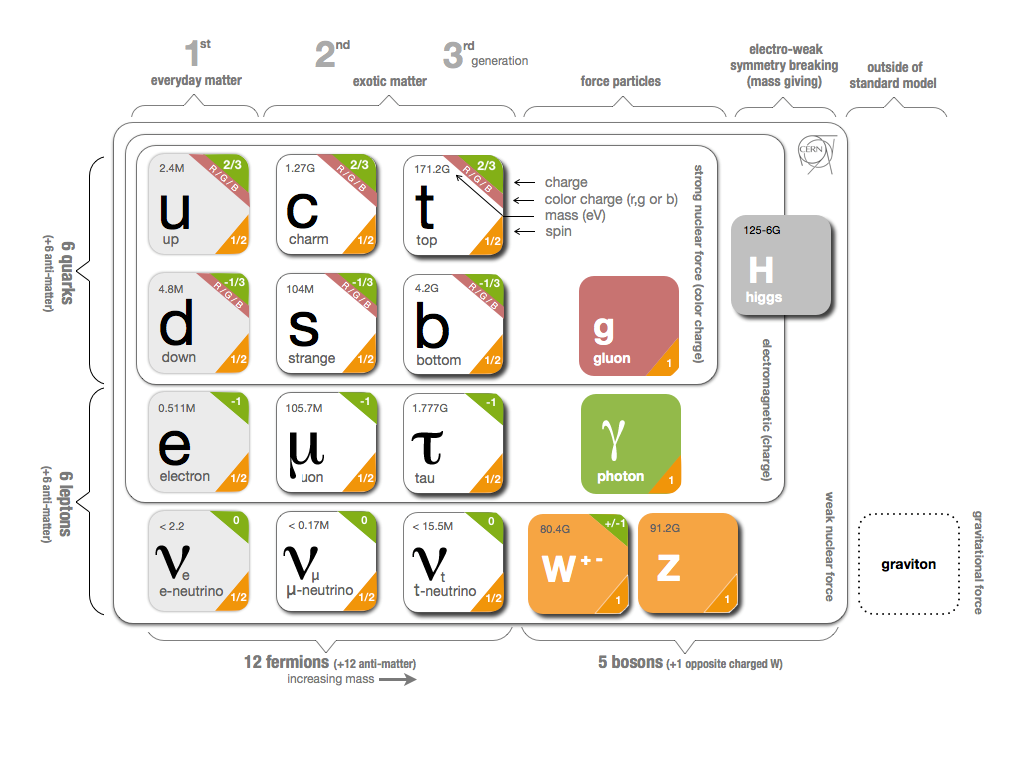
\includegraphics[width=0.9\textwidth]{pics/Intro/standard_model_cern.png}
    \caption{The Standard Model of particles physics: 12 elementary fermions and 5 elementary bosons.
             Plot taken from~\cite{SM_table_CERN}. }
    \label{fig:SM_table}
\end{figure*}

The theory of the SM is formulated in quantum field theory and exhibits rich physics phenomena.
The mathematical construction of the SM is given in the following sections:
Section~\ref{sec:gauge_symmetry} describes the basic formalism of quantum field theory and the idea of gauge symmetry;
Section~\ref{sec:SM_Lagrangian} shows the mathematical description of the SM without the Higgs field and its drawback in describing particle masses;
Section~\ref{sec:Higgs_mech} introduces the Higgs field and its interplay with the gauge fields and fermion fields which allows particles to retain masses;
and Section~\ref{sec:SM_parameters} discusses the free parameters in the SM and the motivation to study the Higgs to muons decay.


\section{Quantum field theory and gauge symmetry}\label{sec:gauge_symmetry}

Symmetry is a key concept in physics. 
A symmetry regarding a certain quantity means the equations of motion do not depend on this quantity
and implies the existence of a conservation law.
For example the symmetries under translations in space and time correspond to the conservations of momenta and energy.

In quantum field theory, the Lagrangian for a free Dirac field is 
\begin{equation}\label{eq:Dirac_Lagrangian}
    \mathcal{L} = \bar{\psi}(x)(i\gamma^{\mu}\partial_{\mu}-m)\psi(x)
\end{equation}
where $\psi(x)$ is the Dirac field,
$\partial_{\mu}$ is the regular partial derivative with Lorentz index $\mu$,
and $m$ is the mass of the Dirac spinor.
$\gamma_{\mu}$ denotes the Dirac matrices
\begin{equation}\label{eq:dirac_matrices}
    \gamma^{0} = \begin{pmatrix}  I_{2} & 0 \\ 0 & -I_{2}    \end{pmatrix} ~,~
    \gamma^{k} = \begin{pmatrix}  0 & \sigma^{k} \\ -\sigma^{k} & 0 \end{pmatrix} ~,~
    \text{with} ~ k = 1,2,3 
\end{equation}
where $I_{2}$ is the $2 \times 2$ identity matrix and $\sigma^{k}$ denotes the Pauli matrices.
\begin{equation}\label{eq:pauli_matrices}
    \sigma_{1} = \begin{pmatrix} 0 & 1 \\ 1 & 0 \end{pmatrix} ~,~
    \sigma_{2} = \begin{pmatrix} 0 & -i \\ i & 0\end{pmatrix} ~,~
    \sigma_{3} = \begin{pmatrix} 1 & 0 \\ 0 & -1\end{pmatrix}
\end{equation}

This Lagrangian is invariant under an internal phase translation
\begin{equation}\label{eq:global_phase}
    \psi(x) \to e^{i\theta_{0}}\psi(x)
\end{equation}
where $\theta_{0}$ is an arbitrary constant.
This is a global symmetry as $\theta_{0}$ is independent from the spacetime location.
A crucial practice in quantum field theory is to promote global symmetries to local symmetries, 
also known as gauge symmetries, under transformations like
\begin{equation}\label{eq:local_phase}
 \psi(x) \to e^{i\theta(x)}\psi(x)
\end{equation}
where $\theta(x)$ is no longer constant but a function of the spacetime coordinates~$x$.
Obviously Equation~\ref{eq:Dirac_Lagrangian} is not invariant under this gauge transformation, 
as the transformation give rise to a new term $\partial_{\mu}\theta(x)$.
The way to achieve gauge invariance is to replace the partial derivative $\partial_{\mu}$ by the covariant derivative, 
through whose construction new interactions are introduced.

The covariant derivative of transformation Equation~\ref{eq:local_phase} is written as
\begin{equation}\label{eq:cov_de_phase}
    D_{\mu} = \partial_{\mu} + \text{i}eA_{\mu}
\end{equation}
where $e$ is an arbitrary constant and $A_{\mu}$ is a new field whose behavior under the same transformation is
\begin{equation}\label{eq:EM_transformation}
    A_{\mu}(x) \to A_{\mu}(x) - \frac{1}{e}\partial_{\mu}\theta(x)
\end{equation}
In fact, this exact formula can be used to describe electromagnetism, 
for which $A_{\mu}$ is the vector potential of the electromagnetic field and $e$ is the electric charge.

Modifying Equation~\ref{eq:Dirac_Lagrangian} with Equation~\ref{eq:cov_de_phase} and adding the EM field term, 
we get a gauge invariant Lagrangian describing a Dirac field interacting with an EM field
\begin{equation}\label{eq:Dirac_EM}
    \mathcal{L} = \bar{\psi}(x)(i\gamma^{\mu}D_{\mu}-m)\psi(x) - \frac{1}{4}F_{\mu\nu}F^{\mu\nu}
\end{equation}
where $F_{\mu\nu}$ is the EM field tensor
\begin{equation}\label{eq:EM_tensor}
    F_{\mu\nu}(x) = \partial_{\mu}A_{\nu}(x) - \partial_{\nu}A_{\mu}(x) 
\end{equation}
The transformation Equation~\ref{eq:local_phase} takes the form of the group U(1) at each point $x$.
Therefore we say the electromagnetic interaction follows a U(1) gauge symmetry.



\section{The standard model Lagrangian}\label{sec:SM_Lagrangian}

Following the formalism in Section~\ref{sec:gauge_symmetry} and knowing there are 6 quarks, 6 leptons, and 4 gauge bosons,
the SM Lagrangian without considering a Higgs boson and without mass terms can be written as:
\begin{equation}\label{eq:SM_Lagrangian}
  \begin{split}
    \mathcal{L} = & \bar{\psi}^{i} (i\gamma^{\mu})(D_{\mu})_{ij}\psi^{j} -
                  - \frac{1}{4} G^{k}_{\mu\nu}G^{k\mu\nu}
                  - \frac{1}{4} W^{a}_{\mu\nu}W^{a\mu\nu}
                  - \frac{1}{4} B_{\mu\nu}B^{\mu\nu}
  \end{split}
\end{equation}
In the equation:
\begin{itemize}
  \item $\psi$ is the fermion field and $D_{\mu}$ is the covariant derivative;
  \item $G^{k}_{\mu\nu}$, $W^{a}_{\mu\nu}$, and $B_{\mu\nu}$ are field strength tensors for the interaction fields 
        corresponding to the groups SU(3), an SU(2), and an U(1), respectively;
  \item $\mu$ and $\nu$ are the Lorentz vector indices. Index $k$ and $a$ are the index of the group generators, $k$ running from 1 to 8, and $a$ running from 1 to 3;
\end{itemize}


This Lagrangian takes the structure of groups SU$(3)_{c} \times$SU$(2)_{L} \times$U$(1)_{Y}$.
The SU$(3)_{c}$ represents the strong interaction with the subscript $c$ standing for color.
The SU$(2)_{L} \times$U$(1)_{Y}$ is the electroweak interaction, 
where the $L$ means it only acts on left-handed fermions
and the $Y$ is the hypercharge associated with the U(1) group.\footnote{The hypercharge $Y$ is not the electric charge $e$ in Equation~\ref{eq:cov_de_phase}.
In fact, for all fermions, the electric charge $Q = T_{3} + Y/2$.}
Here the SU$(2)_{L} \times$U$(1)_{Y}$ cannot be disentangled and viewed separately as the weak interaction and electromagnetic interaction.

The gauge transformations on the fermion field are:
\begin{equation}\label{eq:gauge_fermion}
  \begin{split}
    \text{U(1)}:  & ~~~~ \psi(x) \to  \text{exp}[i\theta_{Y}(x)Y]\psi(x) \\
    \text{SU(2)}: & ~~~~ \psi(x) \to  \text{exp}[i\theta^{a}_{L}(x)T^{a}]\psi(x) \\
    \text{SU(3)}: & ~~~~ \psi(x) \to  \text{exp}[i\theta^{k}_{c}(x)t^{k}]\psi(x) 
  \end{split}  
\end{equation}  
with $D_{\mu}$ taking the form of 
\begin{equation}\label{eq:SM_cov_dev}
  D_{\mu} = \partial_{\mu} - ig^{\prime}B_{\mu}Y - igW^{a}_{\mu}T^{a} - ig_{s}G^{k}_{\mu}t^{k}
\end{equation} 
where $g^{\prime}$, $g$, and $g_{s}$ are field strength coefficients, 
and $Y$, $T^{a}$, and $t^{k}$ are interaction operators, for U(1), SU(2), and SU(3) respectively.
In this construction the transformations on the interaction fields are:
\begin{equation}\label{eq:gauge_interaction}
  \begin{split}
    \text{U(1)}:  & ~~~~  B_{\mu}(x) \to B_{\mu}(x) + \frac{1}{g^{\prime}}\partial_{\mu}\theta_{Y}(x) \\
    \text{SU(2)}: & ~~~~  W^{a}_{\mu}(x) \to  W^{a}_{\mu}(x) + \frac{1}{g}\partial_{\mu}\theta^{a}_{L}(x) + \epsilon^{abc}W^{b}_{\mu}(x)\theta^{c}_{L}(x) \\
    \text{SU(3)}: & ~~~~  G^{k}_{\mu}(x) \to  G^{k}_{\mu}(x) + \frac{1}{g_{s}}\partial_{\mu}\theta^{k}_{c}(x) + f^{klm}G^{l}_{\mu}(x)\theta^{m}_{c}(x)
  \end{split}  
\end{equation}  
Furthermore, the field tensors in Equation~\ref{eq:SM_Lagrangian} are related to the field vectors as
\begin{equation}\label{eq:field_tensor}
  \begin{split}
    \text{U(1)}:  & ~~~~ B_{\mu\nu} = \partial_{\mu}B_{\nu} - \partial_{\nu}B_{\mu} \\
    \text{SU(2)}: & ~~~~ W^{a}_{\mu\nu} = \partial_{\mu}W^{a}_{\nu} - \partial_{\nu}W^{a}_{\mu} + g\epsilon^{abc}W^{b}_{\mu}W^{c}_{\nu} \\
    \text{SU(3)}: & ~~~~ G^{k}_{\mu\nu} = \partial_{\mu}G^{k}_{\nu} - \partial_{\nu}G^{k}_{\mu} + g_{s} f^{klm}G^{l}_{\mu}G^{m}_{\mu} 
  \end{split}
\end{equation}
in which the $\epsilon^{abc}$ and $f^{klm}$ are structure constants of SU(2) and SU(3) governing the relations between group generators
\begin{equation}\label{eq:struture_constant}
  \begin{split}
    [T^{a}, T^{b}] = i\epsilon^{abc}T_{c} \\
    [t^{k}, t^{l}] = if^{klm}t_{m}
  \end{split}
\end{equation}


Equation~\ref{eq:SM_Lagrangian} models the strong and electroweak interactions with matter fields.
However, all particles in this model are massless as there are no mass terms like
\begin{equation}\label{eq:mass_Lagrangian}
    \mathcal{L}_{\text{mass}} = - m_{f} \bar{\psi}^{i}_{f} \psi_{fi}
                                + \frac{1}{2} m^{2}_{G} G_{\mu}G^{\mu}
                                + \frac{1}{2} m^{2}_{W} W_{\mu}W^{\mu}
                                + \frac{1}{2} m^{2}_{B} B_{\mu}B^{\mu}
\end{equation}
None of these terms is gauge invariant.
The gauge boson terms, $m^{2}_{G} G_{\mu}G^{\mu}$, $m^{2}_{W} W_{\mu}W^{\mu}$, and $m^{2}_{B} B_{\mu}B^{\mu}$,
are not gauge invariant because their transformations always introduce new terms depending on the transformations as described in Equation~\ref{eq:gauge_interaction}. 
The reason why the fermion terms, $m_{f} \bar{\psi}^{i}_{f} \psi_{fi}$, are not gauge invariant is not so obvious in this form 
but becomes clear when written in left and right chiral forms: $\psi = \psi_{R} + \psi_{L}$,
in which 
\begin{equation}\label{eq:psi_chiral}
    \psi_{R} = \begin{pmatrix} \psi_{+} \\ 0 \end{pmatrix}, 
    ~\text{and}~
    \psi_{L} = \begin{pmatrix} 0 \\ \psi_{-} \end{pmatrix}
\end{equation}
We also introduce the projection operators:
\begin{equation}\label{eq:projection_op}
    P_{\pm} = \frac{1}{2}(1 \pm \gamma^{5}), ~\text{with}~ \gamma^{5} = i\gamma^{0}\gamma^{1}\gamma^{2}\gamma^{3}
\end{equation}
who act on $\psi$ as
\begin{equation}\label{eq:proj_psi}
  \begin{split}
    P_{+}\psi = \psi_{R}, & ~~~ P_{-}\psi = \psi_{L}, \\
    \bar{\psi}P_{+} = \bar{\psi_{L}}, & ~~~ \bar{\psi}P_{-} = \bar{\psi_{R}}
  \end{split}
\end{equation}
Expanding the term $m\bar{\psi} \psi = m(\bar{\psi_{R}} + \bar{\psi_{L}}) (\psi_{R} + \psi_{L})$,
the terms $\bar{\psi_{R}}\psi_{R}$ and $\bar{\psi_{L}}\psi_{L}$ vanish.
\begin{equation}\label{eq:RR_term}
    \bar{\psi_{R}}\psi_{R} = \bar{\psi} P_{-}P_{+} \psi = \bar{\psi} \frac{1}{4} (1 - (\gamma^{5})^{2}) \psi = 0
\end{equation}
The surviving terms are $m\bar{\psi} \psi = m\bar{\psi_{R}}\psi_{L} + m\bar{\psi_{L}}\psi_{R}$.
The SU$(2)_{L}$ transformation only acts on the left chiral component,
so its phase only appear in $\psi_{L}$ and is not canceled by $\psi_{R}$.
The U$(1)_{Y}$ hypercharge is also different for the left and right components,
leaving the U(1) phase uncanceled.
Therefore the fermion mass terms are not gauge invariant.\footnote{The surviving terms of $\bar{\psi} (i\gamma^{\mu})(D_{\mu})\psi$
are $\bar{\psi_{R}} (i\gamma^{\mu})(D_{\mu})\psi_{R}$ and $\bar{\psi_{L}} (i\gamma^{\mu})(D_{\mu})\psi_{L}$, 
in which the SU$(2)_{L}$ "phase" term cancels properly, making them gauge invariant.}

Therefore, Equation~\ref{eq:mass_Lagrangian} cannot be attached to Equation~\ref{eq:SM_Lagrangian} and all particles must be massless,
which contradicts the experimental findings.
The follow section describes a mechanism to allow particles to retain masses 
through the introduction of a new field component called the Higgs field.


\section{The Higgs mechanism}\label{sec:Higgs_mech}

The Higgs field is a complex scalar field whose potential is:
\begin{equation} \label{eq:Higgs_potential}
    V(\Phi) = - \mu^{2} \Phi^{\dagger}\Phi + \lambda(\Phi^{\dagger}\Phi)^{2}
\end{equation}
in which $\Phi$ is the complex scalar field and $\mu$, $\lambda$ are coefficients.
The shape of the this potential is shown in Figure~\ref{fig:Higgs_potential}. 
Parameter $\lambda$ needs to be positive for $V(\Phi)$ to have a minimum (ground state).
If $\mu^{2} \leqslant 0$, there is a single minimum of $V(\Phi)$ at zero when $|\Phi| = 0$.
If $\mu^{2} > 0$, $V(\Phi)$ can have a degenerate minimum of $-\frac{\mu^{4}}{4\lambda}$ when $\Phi^{\dagger}\Phi = \frac{\mu^{2}}{2\lambda}$.

\begin{figure*}[!htb]
  \centering
  \captionsetup{justification=justified}
  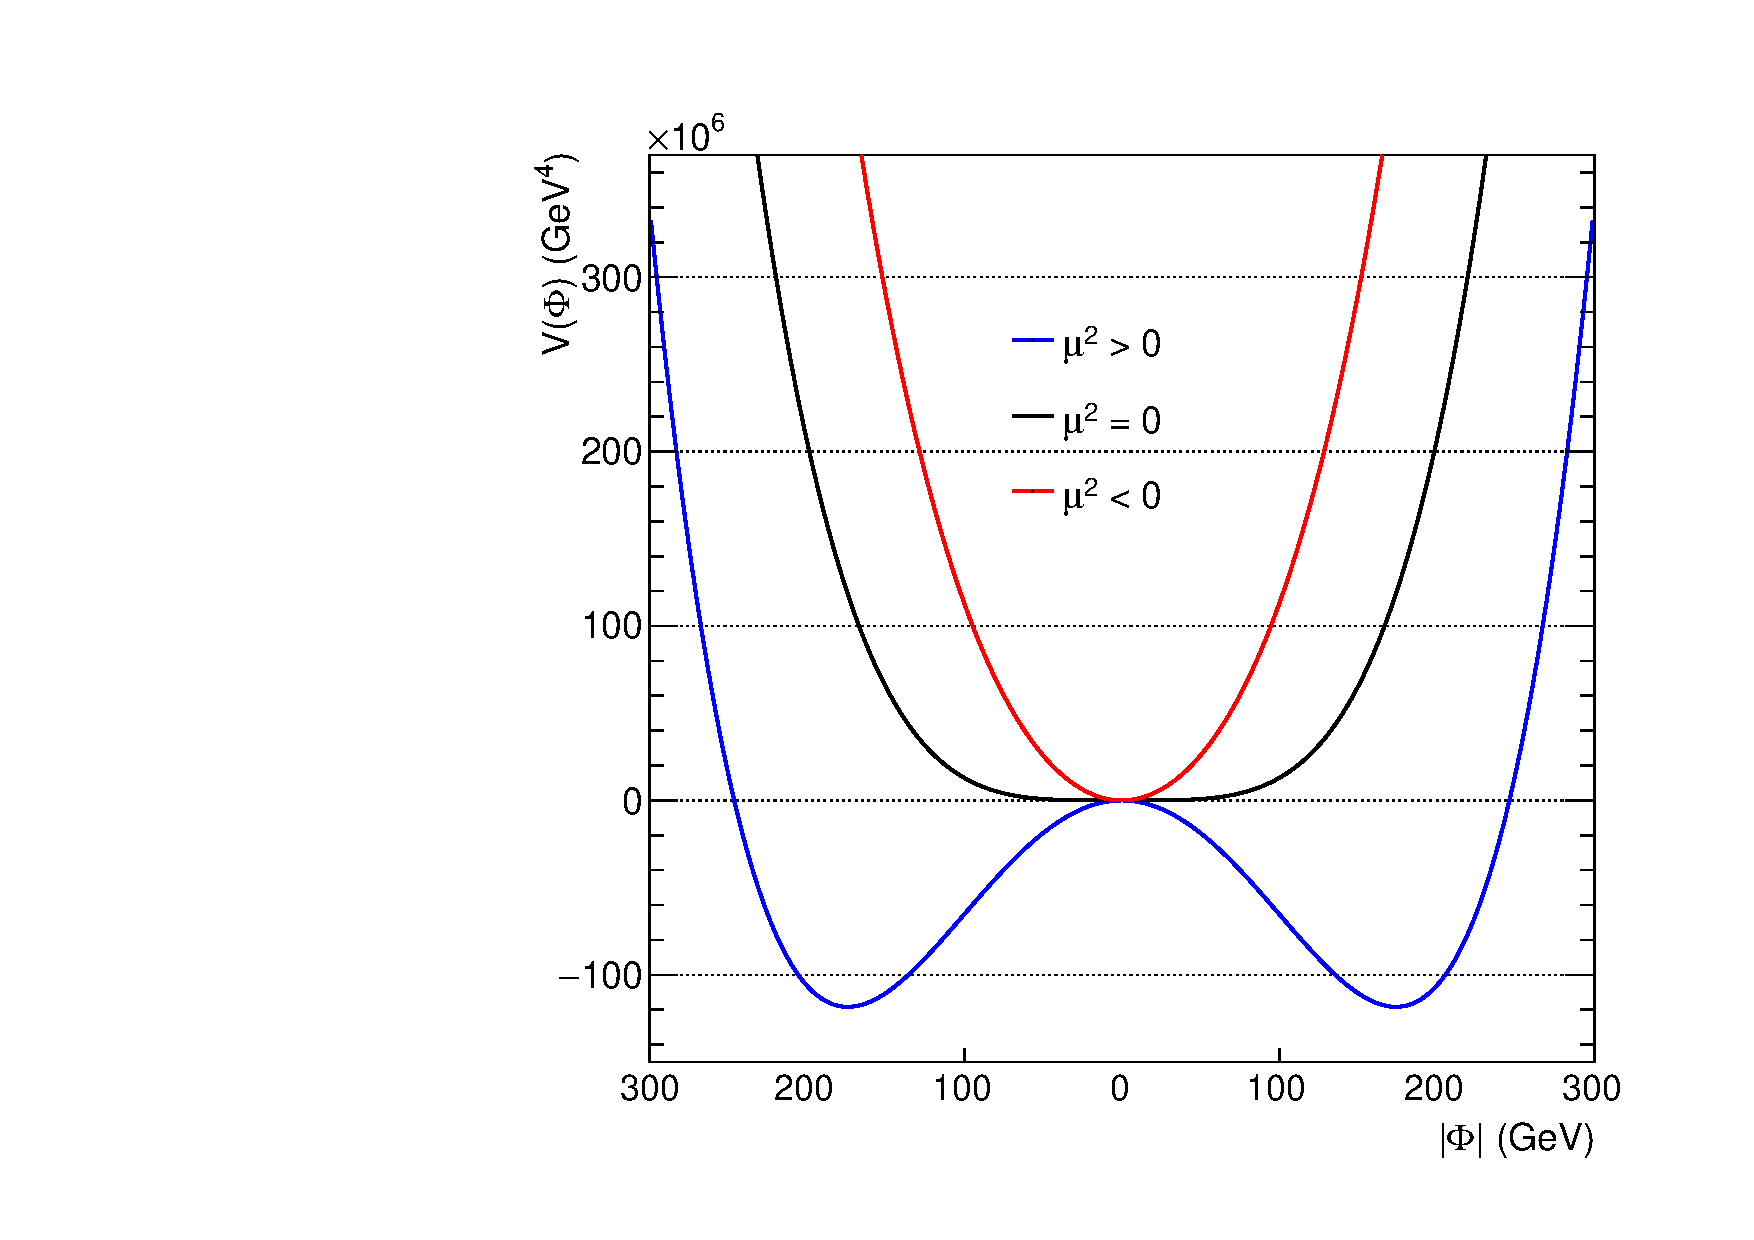
\includegraphics[width=0.6\textwidth]{pics/Intro/Higgs_field.pdf}
  \caption{The shape of the Higgs potential with different $\mu^{2}$ parameter configurations.}
  \label{fig:Higgs_potential}
\end{figure*}

The equation $\Phi^{\dagger}\Phi = \frac{\mu^{2}}{2\lambda}$ represents a circle in the complex plane of $\Phi$.
As $\mu^{2}$ increase from below 0 to above 0, 
the ground state of the field moves from $\Phi = 0$ in an arbitrary direction to a point on the circle $\Phi^{\dagger}\Phi = \frac{\mu^{2}}{2\lambda}$, 
making an asymmetric solution.
This phenomenon is known as the spontaneous symmetry breaking, 
which is also widely observed in physics systems such as the 
bending of a cylindrical rod under axial pressure,
or the cooling of a ferromagnetic material across its Curie temperature.

% Writing the Higgs field together with the simplest gauge field $A_{\mu}$, the Lagrangian is 
% \begin{equation}\label{eq:Higgs_gauge_Lag}
%   \mathcal{L} = |(\partial_{\mu}+ieA_{\mu})\Phi|^{2} -\frac{1}{4}F_{\mu\nu}F^{\mu\nu} + \mu^{2} \Phi^{\dagger}\Phi - \lambda(\Phi^{\dagger}\Phi)^{2}
% \end{equation}
% This Lagrangian itself is invariant under the U(1) gauge symmetry
% \begin{equation}\label{eq:U1_trans}
%     \Phi \to \text{exp}[i\theta(x)]\Phi, ~~~ A_{\mu} \to A_{\mu} - \frac{1}{e} \partial_{\mu}\theta(x)  
% \end{equation}
% but the symmetry breaks as the Higgs field takes a nonzero ground state.
% The fields can be rewritten as
% \begin{equation}\label{eq:Higgs_perturb_form}
%     \Phi(x) \to \frac{1}{\sqrt{2}} (\rho(x)+v)\text{exp}[i\zeta(x)/v], ~~~~~
%     A_{\mu} \to A_{\mu} - \frac{1}{ev} \partial_{\mu}\zeta(x)
% \end{equation}
% where $v = \frac{\mu^{2}}{\lambda}$ is known as the vacuum expectation value,
% $\rho(x)$ and $\zeta(x)$ are scale and phase deviations from this ground state position.
% The Lagrangian now becomes 
% \begin{equation}\label{eq:local_Higgs_gauge_Lag}
%   \begin{split}
%     \mathcal{L} = & -\frac{1}{4}F_{\mu\nu}F^{\mu\nu} + \frac{1}{2} e^{2}v^{2}A_{\mu}A^{\mu} 
%                     + e^{2}v \rho A_{\mu}A^{\mu} + \frac{1}{2} e^{2}\rho^{2}A_{\mu}A^{\mu} \\
%                   & + \frac{1}{2} |\partial_{\mu}\rho|^{2} + \lambda v^{2} \rho^{2} 
%                     - \lambda v \rho^{3} - \frac{1}{4} \lambda \rho^{4} + \frac{1}{4} \lambda v^{4}   
%   \end{split}
% \end{equation}
% In this Lagrangian, a massive gauge boson term $e^{2}v^{2}A_{\mu}A^{\mu}$ appears,
% and the $\rho$ becomes the apparent Higgs field.
% This is a simple example but it already shows rich physics content:
% it describes the coupling between the Higgs boson and the gauge boson $\rho A_{\mu}A^{\mu}$,
% and the 4-point coupling $\rho^{2}A_{\mu}A^{\mu}$,
% as well as the triple and quartic Higgs self-couplings, $\rho^{3}$ and $\rho^{4}$.


Now we look at the SM Lagrangian.
Putting the massless form of Equation~\ref{eq:SM_Lagrangian} together with the Higgs field, it becomes:
\begin{equation}\label{eq:SM_Lagrangian_Higgs}
  \begin{split}
    \mathcal{L} = &  - \frac{1}{4} G^{a}_{\mu\nu}G^{a\mu\nu}
                     - \frac{1}{4} W^{a}_{\mu\nu}W^{a\mu\nu}
                     - \frac{1}{4} B_{\mu\nu}B^{\mu\nu} \\
                  & + |D_{\mu}\Phi|^2 + \mu^{2} \Phi^{\dagger}\Phi - \lambda (\Phi^{\dagger}\Phi)^{2} \\
                  & + \sum_{f} [\bar{\psi}^{f}_{R} (i\gamma^{\mu})(D_{\mu})\psi^{f}_{R} + \bar{\psi}^{f}_{L} (i\gamma^{\mu})(D_{\mu})\psi^{f}_{L}] \\
                  & - \sum_{f} g_{f} [\bar{\psi}^{f}_{R}\Phi^{\dagger}\psi^{f}_{L} + \bar{\psi}^{f}_{L}\Phi\psi^{f}_{R} + \bar{\psi}^{f}_{R}\tilde{\Phi}^{\dagger}\psi^{f}_{L} + \bar{\psi}^{f}_{L}\tilde{\Phi}\psi^{f}_{R}]
  \end{split} 
\end{equation}
where the first and second lines are the gauge field and Higgs field,
the third line is the fermion kinetics written in the chiral form,
and the fourth line is the Yukawa coupling between fermions and the Higgs, also in the chiral form.
The index $f$ in the third and fourth lines just sums all fermions, 
with $g_{f}$ as the coupling strength for each fermion type.
The $\psi_{L}$ are doublets of the SU(2)
\begin{equation}\label{eq:SU2_doublet}
    \psi_{L} = \frac{1}{2} (1+\gamma_{5}) \begin{pmatrix} \nu^{i} \\ l^{i} \end{pmatrix},
    ~~~\text{or}~~~
    \frac{1}{2} (1+\gamma_5) \begin{pmatrix} U^{i} \\ D^{i} \end{pmatrix}
\end{equation}
and $\psi_{R}$ are singlets
\begin{equation}\label{eq:SU2_singlet}
    \psi_{R} =  \frac{1}{2} (1-\gamma_{5}) l^{i}, ~~\frac{1}{2} (1-\gamma_{5}) U^{i}, ~~\text{or}~~\frac{1}{2} (1-\gamma_{5}) D^{i}
\end{equation}
where $\nu^{i}, l^{i}, U^{i}, D^{i}$ are neutrinos, charged leptons, up-type quarks and down-type quarks of three generations.
The existence of right-handed neutrinos is not confirmed by experiments and therefore not assumed in the (simplest) SM.  
The Higgs field is a doublet with 4 total degrees of freedom
\begin{equation}\label{eq:SU2_higgs}
    \Phi = \begin{pmatrix} \Phi^{+} \\ \Phi^{0} \end{pmatrix} 
         = \frac{1}{\sqrt{2}} ~ \begin{pmatrix} \phi^{1}+i\phi^{2} \\ \phi^{3}+i\phi^{4} \end{pmatrix}
    ~,~~
    \tilde{\Phi} = \begin{pmatrix} \Phi^{0\dagger} \\ -\Phi^{-} \end{pmatrix} 
                 = \frac{1}{\sqrt{2}} ~ \begin{pmatrix} \phi^{3}-i\phi^{4} \\ -\phi^{1}+i\phi^{2} \end{pmatrix}     
\end{equation}
By choosing the direction of symmetry breaking to be the real part of $\Phi^{0}$, 
we can make $\phi^{1} = \phi^{2} = \phi^{4} = 0$ at the ground state,
and rewrite the Higgs doublet as
\begin{equation}\label{eq:Higgs_ground}
    \Phi \to \frac{1}{\sqrt{2}} ~\text{exp}[i\theta^{a}_{L}(x)T^{a}] ~\text{exp}[i\theta_{Y}(x)Y] ~\begin{pmatrix} 0 \\ v + \rho \end{pmatrix}
\end{equation} 
with $v = \sqrt{\frac{\mu^{2}}{\lambda}}$ known as the vacuum expectation value,
and $\rho$ as the deviation from the ground state position.


\textbf{Mass of the Higgs boson} comes from the potential term $\mu^{2} \Phi^{\dagger}\Phi - \lambda (\Phi^{\dagger}\Phi)^{2}$,
which expands to 
\begin{equation}\label{eq:potential_expand}
  \mu^{2} \Phi^{\dagger}\Phi - \lambda (\Phi^{\dagger}\Phi)^{2}
  = \lambda v^{2} \rho^{2} - \lambda v \rho^{3} - \frac{1}{4} \lambda \rho^{4} + \frac{1}{4} \lambda v^{4}
\end{equation}
The perturbation $\rho$ acts as the apparent Higgs field.
The term $\lambda v^{2} \rho^{2}$ describes the Higgs mass
\begin{equation}\label{eq:Higgs_mass}
    m_{H} = \sqrt{2\lambda} v
\end{equation}
Furthermore, terms $\rho^{3}$ and $\rho^{4}$ describes important Higgs properties of the triple and quartic self-couplings.

\textbf{Masses of gauge bosons} come from the $|D_{\mu}\Phi|^2$ term, which expands to
\begin{equation}\label{eq:gauge_mass_term}
  \begin{split}
    |D_{\mu}\Phi|^{2} = & \frac{1}{2}|\partial_{\mu}\rho|^{2} 
                        + \frac{1}{8}(v+\rho)^{2} [g^{2}(W^{1}_{\mu}W^{1\mu} + W^{2}_{\mu}W^{2\mu}) + (g^{\prime}B_{\mu}-gW^{3}_{\mu})^{2}] \\
                      = & \frac{1}{8}v^{2} [2g^{2}W^{+}_{\mu}W^{-\mu} + (g^{2}+g^{\prime 2})Z_{\mu}Z^{\mu}] \\
                        & + \frac{1}{4}v\rho [2g^{2}W^{+}_{\mu}W^{-\mu} + (g^{2}+g^{\prime 2})Z_{\mu}Z^{\mu}] \\
                        & + \frac{1}{8}\rho^{2} [2g^{2}W^{+}_{\mu}W^{-\mu} + (g^{2}+g^{\prime 2})Z_{\mu}Z^{\mu}] + \frac{1}{2}|\partial_{\mu}\rho|^{2}
  \end{split}
\end{equation}
In the second step the mass eigenstates of gauge bosons are defined as  
\begin{equation}\label{eq:V_boson_def}
  \begin{split}
    W^{\pm}_{\mu} & = \frac{W^{1}_{\mu} \mp iW^{2}_{\mu}}{\sqrt{2}} \\
    Z_{\mu} & = -\text{sin}\theta_{W} B_{\mu} + \text{cos}\theta_{W} W^{3}_{\mu} \\
    A_{\mu} & = \text{cos}\theta_{W} B_{\mu} + \text{sin}\theta_{W} W^{3}_{\mu}
  \end{split}
\end{equation}
with the Weinberg angle tan$\theta_{W} = g^{\prime}/g$.
The first part in Equation~\ref{eq:gauge_mass_term} becomes the mass terms for the gauge bosons with
\begin{equation}\label{eq:gauge_mass}
  \begin{split}
    m_{W} & = \frac{vg}{2} \\
    m_{Z} & = \frac{v\sqrt{g^{2}+g^{\prime 2}}}{2} \\
    m_{A} & = 0
  \end{split}
\end{equation}
In addition, the second part of Equation~\ref{eq:gauge_mass_term} describes the 3-point couplings between a Higgs boson and a pair of gauge bosons,
while the third part describes the 4-point couplings between a Higgs boson pair and a gauge boson pair.

\textbf{Masses of fermions} come from the Yukawa coupling term in Equation~\ref{eq:SM_Lagrangian_Higgs}.
The term $\bar{\psi}^{f}_{R}\Phi^{\dagger}\psi^{f}_{L} + \bar{\psi}^{f}_{L}\Phi\psi^{f}_{R}$ gives the masses for charged leptons and down-type quarks.
\begin{equation}\label{eq:yukawa_mass}
  \begin{split}
      & -\sum_{f} g_{f} [\bar{\psi}^{f}_{R}\Phi^{\dagger}\psi^{f}_{L} + \bar{\psi}^{f}_{L}\Phi\psi^{f}_{R} ] \\
    = & - \sum_{l^{i}} g_{l^{i}} ~\frac{1}{2\sqrt{2}}~\bar{l}^{i} ~\begin{pmatrix} 0 ,& v+\rho \end{pmatrix} ~\begin{pmatrix} \nu^{i} \\ l^{i} \end{pmatrix}
        - \sum_{l^{i}} g_{l^{i}} ~\frac{1}{2\sqrt{2}}~\begin{pmatrix} \bar{\nu}^{i} ,& \bar{l}^{i} \end{pmatrix} ~\begin{pmatrix} 0 \\ v+\rho \end{pmatrix} ~l^{i} \\
      & - \sum_{D^{i}} g_{D^{i}} ~\frac{1}{2\sqrt{2}}~\bar{D}^{i} ~\begin{pmatrix} 0 ,& v+\rho \end{pmatrix} ~\begin{pmatrix} U^{i} \\ D^{i} \end{pmatrix}
        - \sum_{D^{i}} g_{D^{i}} ~\frac{1}{2\sqrt{2}}~\begin{pmatrix} \bar{U}^{i} ,& \bar{D}^{i} \end{pmatrix} ~\begin{pmatrix} 0 \\ v+\rho \end{pmatrix} ~D^{i} \\
    = & - \frac{1}{\sqrt{2}} \sum_{l^{i}} g_{l^{i}}  (v+\rho) \bar{l}^{i} l^{i}
        - \frac{1}{\sqrt{2}} \sum_{D^{i}} g_{D^{i}}  (v+\rho) \bar{D}^{i} D^{i}    
  \end{split}
\end{equation}
In this equation some calculations are omitted to save space:
the SU(2) phase cancels between $\Phi^{\dagger}$ and $\psi_{L}$, 
the SU(1) phase cancels between $\bar{\psi_{R}}$, $\Phi^{\dagger}$ and $\psi_{L}$ as their hypercharges add up to 0,
and the product of projection operators in $\bar{\psi}_{R}$ and $\psi_{L}$ is 2 and is absorbed in the coefficients.
Similar to Equation~\ref{eq:yukawa_mass}, the term $\bar{\psi}^{f}_{R}\tilde{\Phi}^{\dagger}\psi^{f}_{L} + \bar{\psi}^{f}_{L}\tilde{\Phi}\psi^{f}_{R}$ gives the masses for up-type quarks.
\begin{equation}
    - \sum_{f} g_{f} [\bar{\psi}^{f}_{R}\tilde{\Phi}^{\dagger}\psi^{f}_{L} + \bar{\psi}^{f}_{L}\tilde{\Phi}\psi^{f}_{R}]
    = - \frac{1}{\sqrt{2}} \sum_{U^{i}} g_{U^{i}}  (v+\rho) \bar{U}^{i} U^{i}
\end{equation}
There is no term here for neutrinos as they do not have right-handed components.
Overall, the Yukawa term is summarized as
\begin{equation}\label{eq:Lagrangian_yukawa}
    \mathcal{L}_{\text{Yukawa}} = - \sum_{f} \frac{1}{\sqrt{2}} g_{f} (v\bar{\psi}^{f}\psi^{f} + \rho \bar{\psi}^{f}\psi^{f})
\end{equation}
where the first part is the mass term for fermions, 
and the second part is the interactions between the apparent Higgs field $\rho$ and the fermions.
The fermion mass $m_{f}$ is proportional to its Yukawa coupling strength $g_{f}$
\begin{equation}\label{eq:fermion_mass}
    m_{f} = \frac{vg_{f}}{\sqrt{2}}
\end{equation} 


\section{Parameters of the standard model}\label{sec:SM_parameters}

In the Lagrangian we derived in the last Section, there are 14 unconstrained real parameters (assuming massless neutrinos):
\begin{itemize}
  \item 3 gauge coupling constants $g$, $g^{\prime}$, and $g_{s}$;
  \item 2 Higgs potential shape parameters $\lambda$ and $\mu^{2}$;
  \item 9 Yukawa coupling constants $g_{f}$ for 3 charged leptons and 6 quarks.
\end{itemize}
There are 5 other parameters not elaborated here
\begin{itemize}
  \item 4 parameters in the quark mixing matrix (CKM matrix) which is not elaborated here, including 3 angle parameters and 1 phase parameter;
  \item A parameter for CP violation in the strong interaction.
\end{itemize}
These total 19 parameters determine the exact properties of SM particles and the measurements of them are a key topic of high energy experiments. 
In practice, some other variable sets are frequently used. 
For example, the parameter set $[g, g^{\prime}, \lambda, \mu^{2}, g_{f}]$ is interchangeable with 
the set consisting of the vacuum expectation, and the masses of Higgs, \PW, \PZ, and fermions $[v, m_{H}, m_{W}, m_{Z}, m_{f}]$.


The Higgs boson was first observed at the LHC by ATLAS and CMS Collaborations in 2012~\cite{Aad:2012tfa, Chatrchyan:2012xdj, Chatrchyan:2013lba}.
Various measurements on the Higgs properties have been conducted to verify their agreement with the SM prediction and to put constraints on the free SM parameters.
The latest and most precise measurement of the Higgs mass is $125.38 \pm 0.14$ \GeV, provided by the CMS Collaboration~\cite{2020135425}. 
The Higgs decays to gauge bosons and third-generation fermions (except the top quark) have been observed 
and measured~\cite{Sirunyan:2312121, 201996, Sirunyan:2017exp, PhysRevLett.121.121801, 2018283, PhysRevD.99.072001, 201859, 2019508, Aaboud_2018}.
The Higgs coupling to the top quark has also been measured through the Higgs production process in association with a top quark pair~\cite{PhysRevLett.120.231801, 2018173}.
The Higgs coupling measurements from CMS with the LHC proton-proton collision data collected in 2016 is summarized in Figure~\ref{fig:higgs_2016},
in which, the gauge couplings and Yukawa couplings are expressed by the coupling modifiers 
($\kappa_{\PW}$, $\kappa_{\PZ}$, $\kappa_{t}$, $\kappa_{\tau}$, $\kappa_{b}$, and $\kappa_{\mu}$) in the \kappa-framework~\cite{Heinemeyer:2013tqa}.
This result confirms the proportionality between fermion masses and their coupling strengths to the Higgs boson,
a behavior predicted by the SM in Equation~\ref{eq:fermion_mass}.

The Higgs couplings to fermions of the first and second generations, 
however, are expected to be small and hard to probe.
The study of Higgs to muons decay is of particular importance 
as it is the most experimentally sensitive way to probe Higgs couplings to second-generation fermions.
 

%\begin{table}[!htb]
%  \centering
%  \captionsetup{justification=justified}
%  \topcaption{The branching fractions of the main decay modes of the SM Higgs boson with a mass of 125 \GeV.}
%  \begin{tabular}{lc}
%    \hline
%    Decay mode                 &  Branching fraction \\
%    \hline
%    $\PH \to \Pqb\Paqb$        &  58.4\% \\
%    $\PH \to \PW^{+}\PW^{-}$   &  21.4\% \\
%    $\PH \to gg$               &  8.19\% \\
%    $\PH \to \tau\bar{\tau}$   &  6.26\% \\
%    $\PH \to c\bar{c}$         &  2.89\% \\
%    $\PH \to \PZ\PZ$           &  2.62\% \\
%    $\PH \to \gamma\gamma$     &  0.227\% \\
%    $\PH \to \PZ\gamma$        &  0.153\% \\
%    $\PH \to \mu\bar{\mu}$     &  0.022\% \\
%    \hline
%  \end{tabular}
%  \label{tab:higgs_BR}
%\end{table}


\begin{figure*}[!htb]
    \centering
    \captionsetup{justification=justified}
    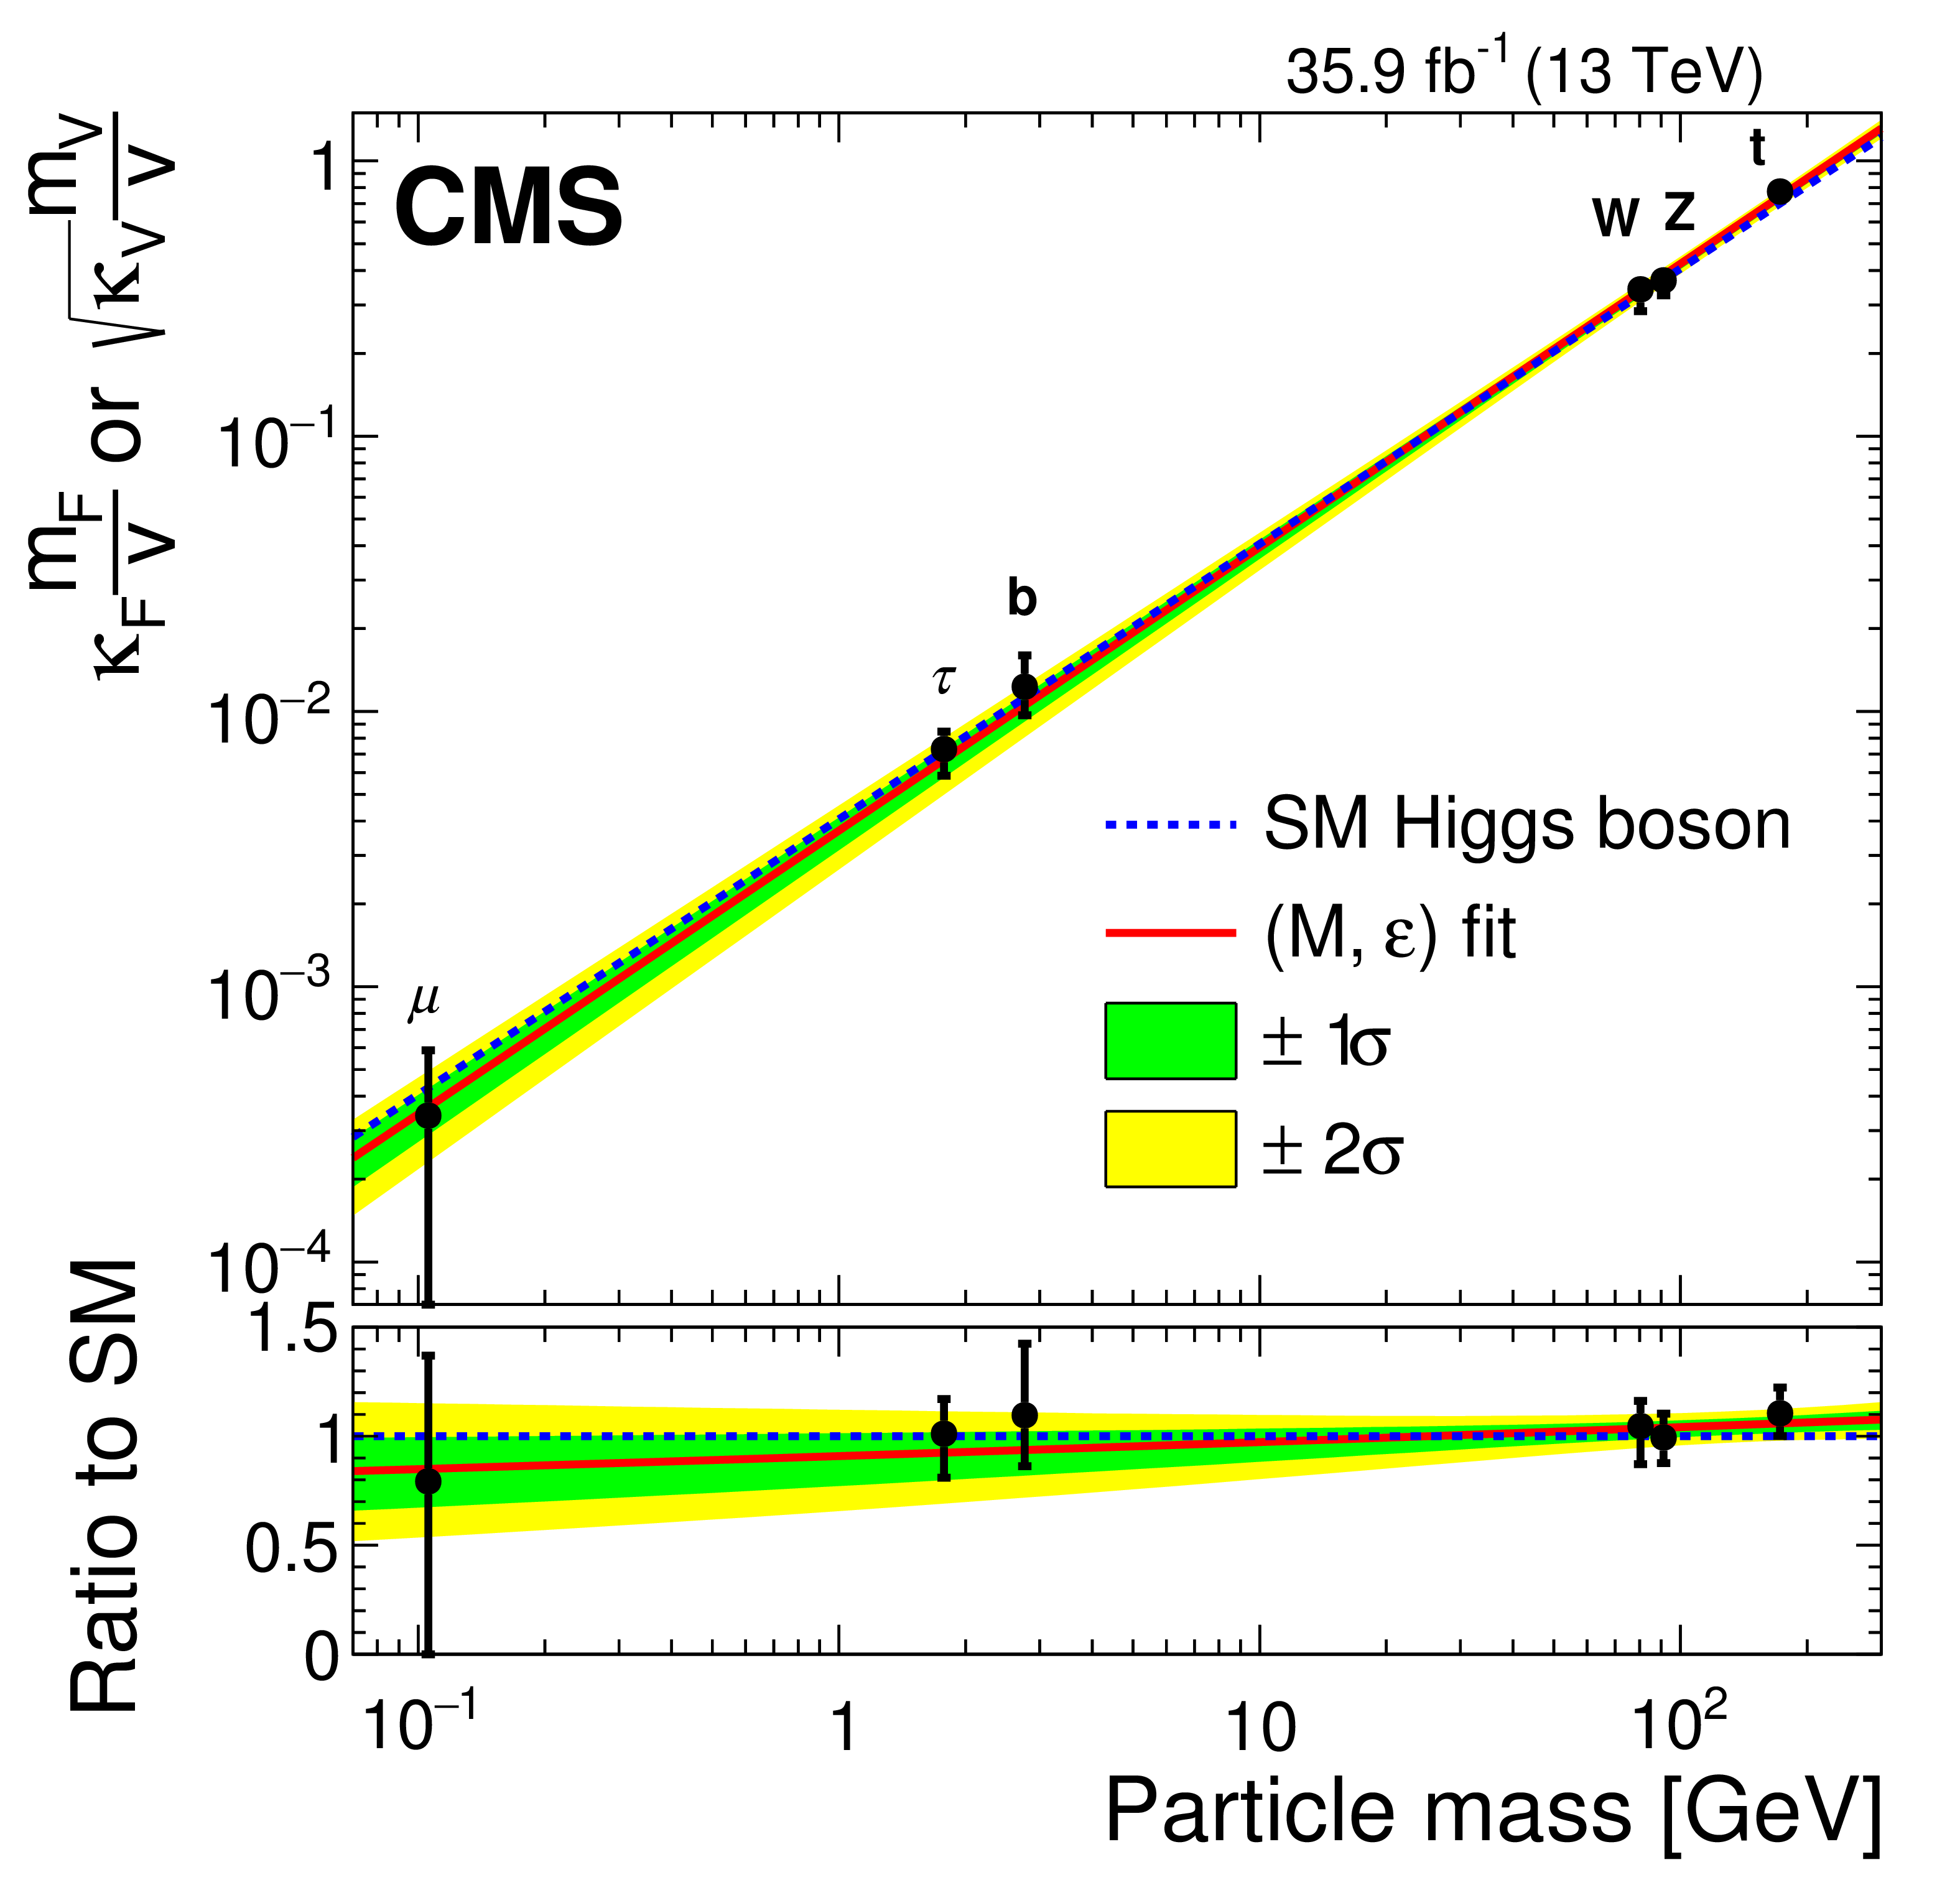
\includegraphics[width=0.60\textwidth]{pics/Intro/higgs_coupling_2016.png}
    \caption{Summary of the CMS measurements on the Higgs coupling to fermions and bosons.
             Plot taken from~\cite{Sirunyan:2640611}. }
    \label{fig:higgs_2016}
\end{figure*}


This thesis presents the recent analysis of the Higgs to muons decay from CMS 
with a focus on the work in the vector boson associated Higgs production channel (VH).
The following chapters are organized as follows:
Chapter~\ref{chp:LHC_CMS} describes the LHC machine and the CMS detector,
Chapter~\ref{chp:hmm_overview} gives an overview of the \hmm analysis 
which is conducted in 4 exclusive event categories targeting different Higgs production modes,
Chapter~\ref{chp:objects} lists the reconstruction of physics objects and the selections on them in the analysis,
Chapter~\ref{chp:muon_corr} details the correction methods and calibration studies on the muon momentum which is crucial to the accuracy of this work,
Chapter~\ref{chp:VH_analysis} reports the full procedures of the analysis in the VH channel,
and Chapter~\ref{chp:hmm_results} summarizes the results from the VH analysis 
as well as the combined results of all 4 analysis channels. 
\chapter{The LHC and CMS}

\section{The Large Hadron Collider}

\section{The Compact Muon Solenoid experiment}

\section{Trigger system in CMS}

\section{Level-1 Trigger}

\chapter{Overview of the Search of \texorpdfstring{\hmm}{H to Muons} Decay at CMS}\label{chp:hmm_overview}
% Need to use \textorpdfstring{} so it also shows in pdf bookmarks 

As described in Section~\ref{sec:SM_parameters}, the Yukawa couplings between the Higgs boson and the elementary fermions are essential parameters to the SM.
The Higgs couplings to fermions of the first and second generations are hard to probe because the Higgs boson decay ratios to these light fermions are small.
At the LHC, the most experimentally sensitive way to probe such light Yukawa couplings is the study of the \hmm decay.
Prior to this work, searches for the \hmm decay has been conducted using $pp$ collision data collected at center-of-mass energies of 7, 8, and 13 \TeV
by CMS~\cite{2015184, PhysRevLett.122.021801} and ATLAS~\cite{201468, PhysRevLett.119.051802, Aad:2020xfq},
among which the most sensitive result~\cite{PhysRevLett.122.021801} is reported by CMS with an observed (expected in absence of \hmm decay) upper limit of 2.9 (2.2) times the 
SM prediction of the Higgs boson production and \brhmm, at the 95\% confidence level (CL).
This thesis reports the latest \hmm analysis based on 137~\invfb of data collected by CMS from 2016 to 2018~\cite{Sirunyan_2021}.

The search for the \hmm decay, in a nutshell, is a struggle to make the signal events stand out from the vast backgrounds with statistical significance.
The \hmm decay has a branching ratio of ${\brhmm = 2.18 \times 10^{-4}}$, 
which corresponds to an expectation of about 1000 event instances in the data collected by CMS from 2016 to 2018.
In contrast, these 1000 signal events are accompanied by millions of events produced through other processes (background events) that mimic their experimental signature.
The most important difference between the signal events and the background events lies in the dimuon invariant mass (\mmm) distribution, illustrated in Figure~\ref{fig:dimuon_mass_shapes}.
The SM Higgs boson has a low production cross section and a narrow natural width, making a small sharp peak near 125~\GeV.
The background events are dominated by the $\PZ/\gamma^{*} \to \mu\mu$ process (Drell-Yan process), 
which peaks at 91.2~\GeV in the \mmm spectrum and leaves a smooth falling tail around 125~\GeV.
The overall signal-to-background ratio (\SoB) between 120 and 130~\GeV is about 1/500 in the 2016-2018 CMS data.

\begin{figure}[!htb]
    \centering
%    \captionsetup{justification=justified}
    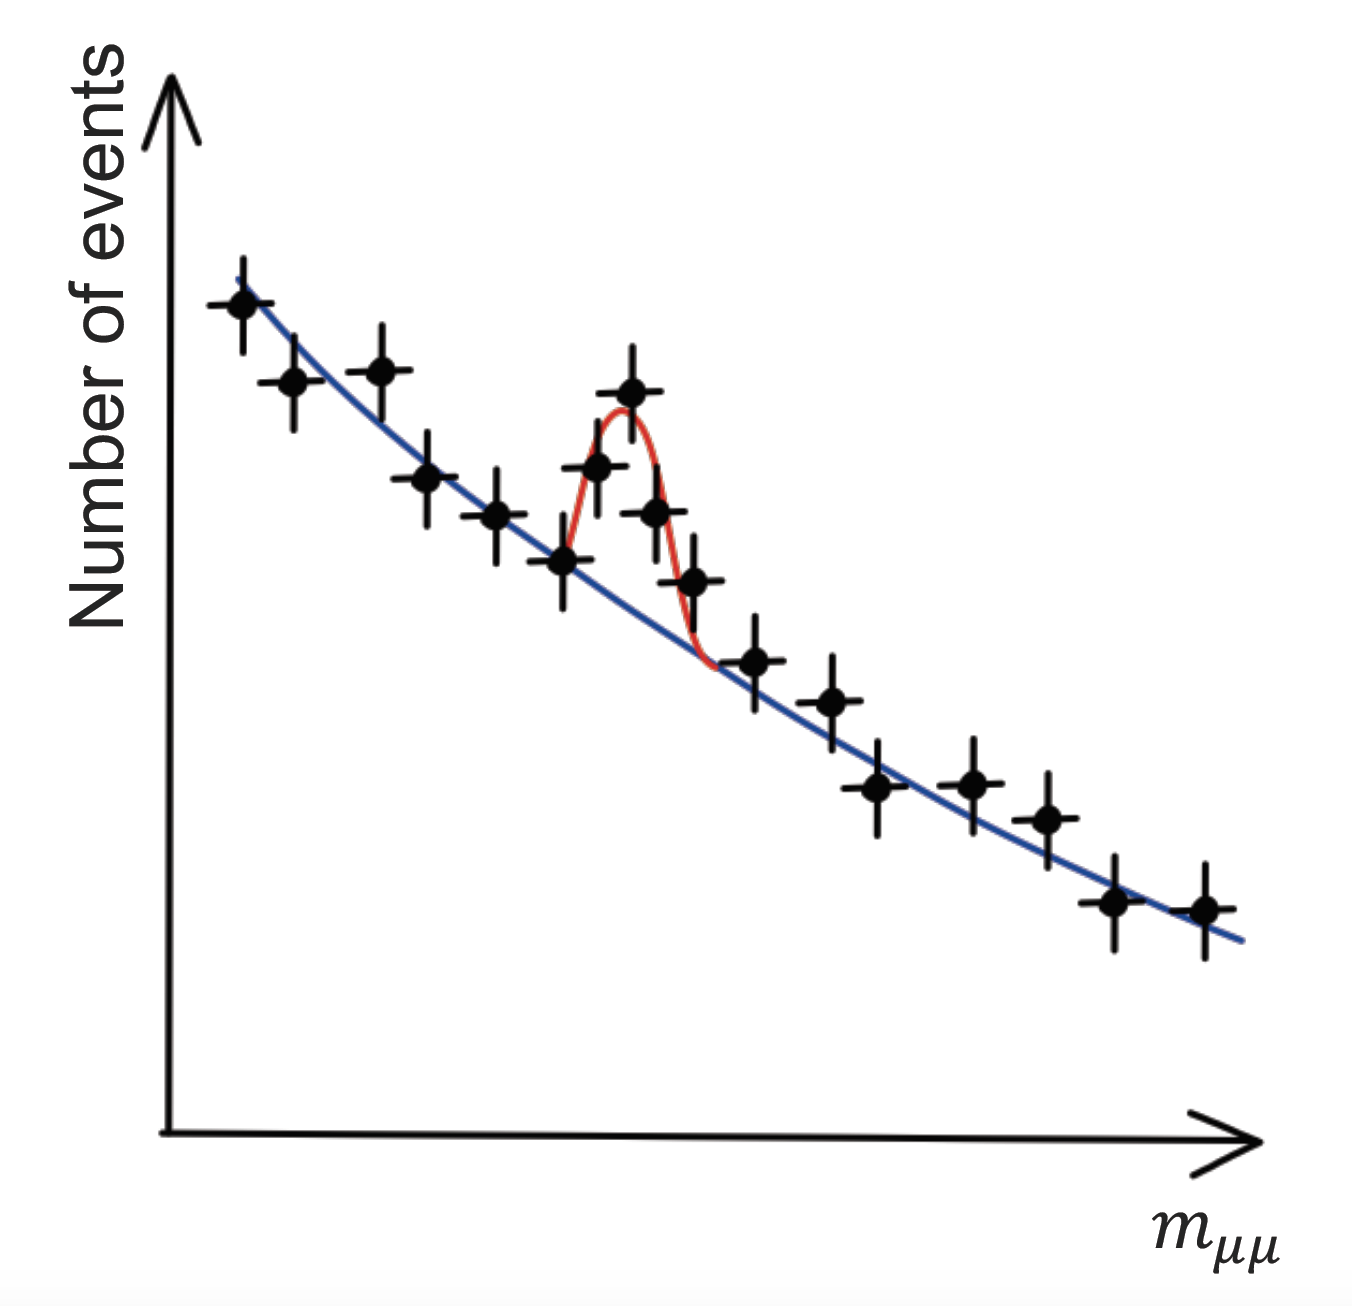
\includegraphics[width=0.6\textwidth]{pics/hmm_mass_sketch.png}
    \caption{A conceptual plot for the dimuon mass shapes for the signal and the background. 
             The blue line shows the expected background shape, while the red line shows the expected signal shape on top of it.}
    \label{fig:dimuon_mass_shapes}
\end{figure}

This \SoB can be enhanced based on further kinematic distinctions between various signal and background processes.
The Higgs boson is produced via several production modes.
The four main modes, ordered by their cross sections, are gluon fusion (\ggH), vector boson fusion (\qqH or qqH), 
associated production with a weak vector boson (\VH), and associated production with a pair of top quarks (\ttH). 
The Feynman diagrams for these main production modes are shown in Figure~\ref{fig:main_higgs_modes}.
The minor production modes include associated production with a pair of bottom quarks (\bbH),
associated production with a \PZ boson through gluon fusion (\ggZH), 
associated production with a top quark and a \PW boson (\tHW), 
and associated production with a top quark and a light quark (\tHq). 
The Feynman diagrams for these minor production modes are shown in Figure~\ref{fig:minor_higgs_modes}.
Table~\ref{tab:signal_xsec} summarizes the cross sections for all these production modes, 
along with the expected number of events in the 137~\invfb data.

\begin{figure}[!htb]
    \centering 
    \captionsetup{justification=centering}
    \begin{subfigure}[b]{0.45\textwidth} % b for bottom alignment so caption is at the same height
        \centering
        \feynmandiagram[horizontal=g1 to t1, horizontal=t2 to h] {
            g1 [particle = \Pg] -- [gluon] t1,
            t1 -- [fermion, edge label = \Pqt] t2 -- [fermion, edge label = \Pqt] t3 -- [fermion, edge label = \Pqt] t1,
            g2 [particle = \Pg] -- [gluon] t3,
            t2 -- [scalar] h [particle = \PH],
            g1 -- [draw=none] g2,
        };

        \caption*{\ggH}
    \end{subfigure} 
    %to put these two diagrams side by side. no empty line in between these two blocks, otherwise it indicates an empty line in the pdf
    \begin{subfigure}[b]{0.45\textwidth}
        \centering
        \feynmandiagram[horizontal=b to h]{
            q1 [particle = $\Pq_{1}$] -- [fermion] a -- [fermion] aq1 [particle = $\Pq^\prime_{1}$],
            a -- [boson, edge label = \PV] b -- [boson, edge label = \PV] c,
            b -- [scalar] h [particle = \PH],
            aq2 [particle = $\Pq_{2}$] -- [fermion] c -- [fermion] q2 [particle = $\Pq^\prime_{2}$],

            q1 -- [draw = none] n -- [draw = none] aq2,
            a -- [draw = none] c,
            aq1 -- [draw = none] h -- [draw = none] q2,

        };
        \caption*{\qqH}
    \end{subfigure}

    \begin{subfigure}[b]{0.45\textwidth}
        \centering
        \feynmandiagram[horizontal=a to b] {
            q [particle = \Pq] -- [fermion] a -- [anti fermion] aq [particle = $\Pq^\prime$],
            a -- [boson, edge label = \PV] b,
            v [particle = \PV] -- [boson] b -- [scalar] h [particle = \PH],
        };
        \caption*{\VH}
    \end{subfigure}
    \begin{subfigure}[b]{0.45\textwidth}
        \centering
        \feynmandiagram[horizontal=b to h]{
            g1 [particle = \Pg] -- [gluon] a -- [fermion] t1 [particle = \Pqt],
            a -- [anti fermion, edge label = \Paqt] b -- [anti fermion, edge label = \Pqt] c,
            b -- [scalar] h [particle = \PH],
            g2 [particle = \Pg] -- [gluon] c -- [anti fermion] t2 [particle = \Paqt],

            g1 -- [draw = none] n -- [draw = none] g2,
            a -- [draw = none] c,
            t1 -- [draw = none] h -- [draw = none] t2,
        };
        \caption*{\ttH}
    \end{subfigure}
    \caption{Main production modes of the Higgs boson.}
    \label{fig:main_higgs_modes}
\end{figure}



\begin{figure*}[!htb]
    \centering
    \captionsetup{justification=centering}
    \begin{subfigure}[b]{0.45\textwidth}
        \centering
        \feynmandiagram[horizontal=b to h]{
            g1 [particle = \Pg] -- [gluon] a -- [fermion] b1 [particle = \Pqb],
            a -- [anti fermion, edge label = \Paqb] b -- [anti fermion, edge label = \Pqb] c,
            b -- [scalar] h [particle = \PH],
            g2 [particle = \Pg] -- [gluon] c -- [anti fermion] b2 [particle = \Paqb],

            g1 -- [draw = none] n -- [draw = none] g2,
            a -- [draw = none] c,
            b1 -- [draw = none] h -- [draw = none] b2,
        };
        \caption*{\bbH}
    \end{subfigure}
    \begin{subfigure}[b]{0.45\textwidth}
        \centering
        \feynmandiagram[horizontal=a to b] {
            g [particle = \Pg] -- [gluon] a -- [anti fermion] qb [particle = \Pqb],
            a -- [fermion, edge label = \Pqb] b,
            w [particle = $\PW^{-}$] -- [boson] b -- [fermion, edge label = \Pqt] th -- [fermion] t [particle = \Pqt],
            th -- [scalar] h [particle = \PH],
            t -- [draw = none] h -- [draw = none] w, 
        };
        \caption*{\tHW}
    \end{subfigure}

    \begin{subfigure}[b]{0.45\textwidth}
        \centering
        \feynmandiagram[vertical=a to b] {
            q [particle = \Pq] -- [fermion] a -- [fermion] aq [particle = \Pq'],
            a -- [boson, edge label = \PW] b,
            qb [particle = \Pqb] -- [fermion] b -- [fermion, edge label = \Pqt] c,
            c -- [scalar] h [particle = \PH],
            c -- [fermion] t [particle = \Pqt],
            q -- [draw = none] n -- [draw = none] qb,
            aq -- [draw = none] h -- [draw = none] c,
            aq -- [draw = none] h -- [draw = none] t,
        };
        \caption*{\tHq}
    \end{subfigure}
    \begin{subfigure}[b]{0.45\textwidth}
        \centering
        \feynmandiagram[horizontal=b to h]{
            q1 [particle = \Pq] -- [fermion] a -- [fermion] q2 [particle = $\Pq^\prime$],
            a -- [boson, edge label = \PW] b -- [boson, edge label = \PW] c,
            b -- [scalar] h [particle = \PH],
            qb [particle = \Pqb] -- [fermion] c -- [fermion] qt [particle = \Pqt],

            q1 -- [draw = none] n -- [draw = none] qb,
            a -- [draw = none] c,
            q2 -- [draw = none] h -- [draw = none] qt,
        };
        \caption*{\tHq}
    \end{subfigure}

    \begin{subfigure}[b]{0.45\textwidth}
        \centering
        \feynmandiagram[horizontal=g1 to q1, horizontal=q2 to z] {
            g1 [particle = \Pg] -- [gluon] q1,
            q1 -- [fermion, edge label' = \Pq] q2 -- [fermion, edge label' = \Pq] q3 -- [fermion, edge label' = \Pq] q1,
            g2 [particle = \Pg] -- [gluon] q3,
            q2 -- [boson, edge label = \PZ] z ,
            z -- [boson] z2 [particle = \PZ],
            z -- [scalar] h [particle = \PH],
            g1 -- [draw=none] g2,
        };
        \caption*{\ggZH}
    \end{subfigure} 
    \begin{subfigure}[b]{0.45\textwidth}
        \centering
        \feynmandiagram[horizontal=t1 to t2] {
            g1 [particle = \Pg] -- [gluon] t1 -- [fermion, edge label = \Pqt] t2 -- [boson] z [particle = \PZ],
            g2 [particle = \Pg] -- [gluon] t4 -- [anti fermion, edge label = \Pqt] t3 -- [scalar] h [particle = \PH],
            t1 -- [anti fermion, edge label = \Pqt] t4,
            t2 -- [fermion, edge label = \Pqt] t3,
            g1 -- [draw = none] g2,
            z -- [draw = none] h,
        };
        \caption*{\ggZH}
    \end{subfigure} 
    \caption{Examples of minor Higgs boson production modes.}
    \label{fig:minor_higgs_modes}
\end{figure*}

\begin{table}[!htb]
    \centering
%    \captionsetup{justification=justified}
    \topcaption{Production modes of the Higgs boson in $pp$ collisions at the LHC, their cross sections for $\mh = 125 \GeV$, 
                and the corresponding expected number of \hmm decays in the dataset for this analysis 
                (the cross sections multiplying \brhmm and the integrated luminosity ($137 \invfb$). 
                The leptons ($\ell$) in the table refer to electrons or muons.}
    \begin{tabular}{lccc}
        \hline
        signal mode         & decay mode                & Cross section (\pb)   & Expected \hmm events \\
        \hline
        \ggH                & inclusive                 & 48.58                 & 1450 \\
        \qqH                & inclusive                 & 3.782                 & 113 \\
        \WH                 & inclusive                 & 1.373                 & 41.0 \\
                            & $\PW\to\ell\nu$           & 0.293                 & 8.75 \\
%                            & $\PW\to$ hadrons          & 0.926                 & 27.6 \\
        ${\Pq\Pq\to\PZ\PH}$ & inclusive                 & 0.761                 & 22.7 \\
                            & $\PZ\to\ell\ell$          & 0.051                 & 1.53 \\
%                            & $\PZ\to\nu\nu$            & -                     & - \\
%                            & $\PZ\to$ hadrons          & -                     & - \\
        \ggZH               & inclusive                 & 0.123                 & 3.67 \\
                            & $\PZ\to\ell\ell$          & 0.008                 & 0.25 \\
%                            & $\PZ\to\nu\nu$            & -                     & - \\
%                            & $\PZ\to$ hadrons          & -                     & - \\
        \ttH                & inclusive                 & 0.507                 & 15.1 \\
                            & $\geq 1~\Pqt\to$ leptons  & 0.193                 & 5.76 \\
                            & Both $\Pqt\to$ hadrons    & 0.230                 & 6.86 \\
        \hline
        sum of above        & inclusive                 & 55.13                 & 1646 \\
        \hline
        \bbH                & inclusive                 & 0.488                 & 14.6 \\
        \tHq                & inclusive                 & 0.074                 & 2.21 \\
        \tHW                & inclusive                 & 0.015                 & 0.45 \\
        \hline
        sum of all          & inclusive                 & 55.70                 & 1663 \\
        \hline
    \end{tabular}
    \label{tab:signal_xsec}
\end{table}

To fully exploit the kinematic profiles of different production modes, 
the \hmm analysis is performed in four event categories targeting each of the four main modes,
with the analysis procedures optimized separately in each category.
No dedicated category is made for the minor signal modes, 
either because they have very similar features to one of the main modes, 
or because their cross sections are too small to be statistically significant.
This chapter gives an overview of the full \hmm analysis, 
with Section~\ref{sec:data_mc_samples} describing the data and simulation samples used in the analysis, 
and Section~\ref{sec:hmm_cat_and_strategy} explaining the analysis strategies in the four exclusive categories.


\bigskip
\section{Data and Simulation Samples}\label{sec:data_mc_samples}

This analysis uses the $pp$ collision data collected by CMS from 2016 to 2018,
corresponding to an integrated luminosity of 137\invfb.
The triggers used in this analysis are the single muon HLT triggers, 
which impose some loose isolation requirements and a \pt threshold on the HLT muon candidates.
The \pt threshold is 24/27/24 \GeV for 2016/2017/2018 datasets.
The efficiencies of these triggers are above 90\% for single muons above the trigger thresholds,
and the overall efficiency for events with two muons is close to 100\%.

Simulations of signal and background processes are produced by Monte Carlo (MC) event generators.
The generators are listed for different processes in the rest of this section.
All simulated samples except the EW~$\PZ+jj$ samples use \PYTHIA 8.2~\cite{SJOSTRAND2015159} to model the parton showering (PS), 
hadronization, and the underlying event (UE), while the EW~$\PZ+jj$ samples use \HERWIGpp and \HERWIGSeven~\cite{Bellm:2015jjp} for the same purpose.
The effect of pileup is modeled by overlaying simulated inelastic $pp$ collisions on the hard-scattering event.
The generated events are processed through a simulation of the CMS detector based on \GEANTfour~\cite{AGOSTINELLI2003250}
and are reconstructed with the same algorithms that are used for data.

\bigskip
\subsection{Simulation of Signal Processes}
The \ggH signal process is simulated at next-to-leading order (NLO) accuracy in perturbative QCD, using both the \MGvATNLO~v2.4.2~\cite{Alwall:2014hca}
and \POWHEG~v2.0~\cite{Nason_2004, Frixione_2007, Alioli:2010xd, Bagnaschi:2011tu} event generators. 
The \pt distribution of the Higgs boson in \ggH process is then reweighted to match the \POWHEG~\textsc{nnlops} prediction~\cite{Hamilton:2013fea,Hamilton:2015nsa}. 
The \qqH, \WH, \qqZH, and \ttH processes are simulated with \POWHEG~v2.0~\cite{Nason:2009ai,Luisoni:2013kna,Hartanto:2015uka} at NLO precision in QCD. 
The \bbH process is simulated at NLO precision in QCD with \POWHEG.
the \tHq, and \tHW processes are generated at leading order (LO) with the \MGvATNLO generator.
The \ggZH process is simulated at LO with the \POWHEG generator.
Simulated signal events are generated, for each production mode, at \mh values of 120, 125, and 130~\GeV.
A table summarizing the simulation for signals is shown in Table~\ref{tab:sig_samples}.

\begin{table}[!htb]
    \centering
    \captionsetup{justification=centering}
    \topcaption{Summary of the specification for the simulated Higgs signal samples.}
    \resizebox{\textwidth}{!}{\begin{tabular}{lcccc}
        \hline
        Sample                 &Generator (Perturbative order)    &Parton Shower          &Cross section      &Additional corrections\\
        \hline
        \ggH                   &\MGvATNLO (NLO QCD)               &\PYTHIA                &N3LO QCD, NLO EW   &$\pt(\PH)$ from \textsc{nnlops}\\
        \qqH                   &\POWHEG (NLO QCD)                 &\PYTHIA dipole shower  &NNLO QCD, NLO EW   & -\\
        ${\Pq\Pq\to\PV\PH}$    &\POWHEG (NLO QCD)                 &\PYTHIA                &NNLO QCD, NLO EW   & -\\
        \ggZH                  &\POWHEG (LO)                      &\PYTHIA                &NNLO QCD, NLO EW   & -\\
        \ttH                   &\POWHEG (NLO QCD)                 &\PYTHIA                &NLO QCD, NLO EW    & -\\
        \bbH                   &\POWHEG (NLO QCD)                 &\PYTHIA                &NLO QCD            & -\\
        \tHq                   &\MGvATNLO (LO)                    &\PYTHIA                &NLO QCD            & -\\
        \tHW                   &\MGvATNLO (LO)                    &\PYTHIA                &NLO QCD            & -\\
        \hline
    \end{tabular}}
    \label{tab:sig_samples}
\end{table}

Expected signal yields are normalized to the production cross sections and \brhmm values taken from the recommendations of LHC Yellow Report~\cite{deFlorian:2016spz}.
The \ggH production cross section is computed at next-to-next-to-NLO (N3LO) precision in QCD, and at NLO in EW theory~\cite{Anastasiou:2016cez}. 
The cross section of Higgs boson production in the VBF~\cite{Cacciari:2015jma} and ${\Pq\Pq\to\PV\PH}$~\cite{Brein:2003wg} modes is calculated at next-to-NLO (NNLO) in QCD, 
including NLO EW corrections, while the \ttH cross section is computed at NLO in QCD and EW theory~\cite{Dawson:2003zu,Frixione:2014qaa}. 
The \bbH, \tHq, and \tHW cross sections are computed at NLO in QCD without including higher-order EW corrections~\cite{deFlorian:2016spz,Demartin:2015uha,Demartin:2016axk}. 
The \hmm partial width is computed with \textsc{hdecay}~\cite{Djouadi:1997yw,Spira:1997dg} at NLO in QCD and EW theory.

\bigskip
\subsection{Simulation of Background Processes}
The background is modeled considering various SM processes, summarized in Table~\ref{tab:bkg_samples}.
The main background in the \ggH and \qqH categories is the DY process, which is simulated at NLO in QCD using the \MGvATNLO generator. 
The corresponding cross section is calculated with \FEWZ~v3.1b2~\cite{Li:2012wna} at NNLO in QCD and NLO accuracy in EW theory. 
The EW production of a $\PZ$ boson in association with two jets ($\PZ+jj$) is an important background in the VBF category. 
This process is simulated at LO using the \MGvATNLO~v2.6.5 generator. 
The $\PW\PZ$, ${\Pq\Paq\to\PZ\PZ}$, and $\PW\PW$ processes, which constitute the main backgrounds in the $\PV\PH$ category, 
are simulated at NLO in QCD using either the \POWHEG or \MGvATNLO generators. 
Their production cross sections are corrected with the NNLO/NLO $K$ factors taken from Refs.~\cite{Grazzini:2017ckn},~\cite{Grazzini:2015hta}, and~\cite{Gehrmann:2014fva}. 
The gluon-initiated loop-induced ZZ process (\ggZZ) is simulated with the \MCFM~v7.0 generator~\cite{Campbell:2011bn} at LO 
and the corresponding production cross section is corrected to match higher-order QCD predictions, following the strategy detailed in Ref.~\cite{Sirunyan:2017exp}. 
Minor contributions from triboson processes ($\PW\PW\PW$, $\PW\PW\PZ$, $\PW\PZ\PZ$, and $\PZ\PZ\PZ$) are also taken into account and are simulated at NLO in QCD using the \MGvATNLO generator. 
The main backgrounds in the \ttH category involve the production of top quarks. 
The $\Pqt\Paqt$ background is simulated with NLO precision in QCD using the \POWHEG generator, and its cross section is obtained from the \TOPpp~v2.0~\cite{Czakon:2011xx} prediction 
that includes NNLO corrections in QCD and resummation of next-to-next-to-leading logarithmic (NNLL) soft gluon terms. 
The single top quark processes are simulated at NLO in QCD via either \POWHEG or \MGvATNLO and their cross sections are computed, 
at the same order of precision, using \textsc{hathor}~\cite{Kant:2014oha}. 
Finally, contributions from the $\Pqt\Paqt\PZ$, $\Pqt\Paqt\PW$, $\Pqt\Paqt\PW\PW$, ${\Pqt\Paqt\Pqt\Paqt}$, and \tZq processes 
are also considered and are simulated using the \MGvATNLO generator at NLO precision in QCD. 
For the simulated samples corresponding to the 2016 (2017--2018) data-taking periods, the NNPDF~v3.0~(v3.1) NLO (NNLO) parton distribution functions (PDFs) are used~\cite{Ball:2014uwa,Ball:2017nwa}. 
For processes simulated at NLO (LO) in QCD with the \MGvATNLO generator, events from the matrix element (ME) characterized by different parton multiplicities are merged via the FxFx (MLM) prescription~\cite{Alwall:2007fs,Frederix:2012ps}.


\begin{table}[!htb]
    \centering
    \captionsetup{justification=centering}
    \topcaption{Summary of the specification for the simulated background samples.}
    \resizebox{\textwidth}{!}{\begin{tabular}{lcccc}
        \hline
        Sample                              &Generator (Perturbative order)    &Parton Shower          &Cross section      &Additional corrections\\
        \hline
        Drell-Yan                           &\MGvATNLO (NLO QCD)               &\PYTHIA                &NNLO QCD, NLO EW   & -\\
        Zjj-EW                              &\MGvATNLO (LO)                    &\HERWIGpp/\HERWIGSeven &LO                 & -\\
        $\Pqt\Paqt$                         &\POWHEG (NLO QCD)                 &\PYTHIA                &NNLO QCD           & -\\
        Single top quark                    &\POWHEG/\MGvATNLO (NLO QCD)       &\PYTHIA                &NLO QCD            & -\\
        Diboson ($\PV\PV$)                  &\POWHEG/\MGvATNLO (NLO QCD)       &\PYTHIA                &NLO QCD            & NNLO/NLO $K$ factors\\
        \ggZZ                               &\MCFM (LO)                        &\PYTHIA                &LO                 & NNLO/LO $K$ factors\\
        $\Pqt\Paqt\PV$, $\Pqt\Paqt\PV\PV$   &\MGvATNLO (NLO QCD)               &\PYTHIA                &NLO QCD            & -\\
        Triboson ($\PV\PV\PV$)              &\MGvATNLO (LO)                    &\PYTHIA                &NLO QCD            & -\\
        \hline
    \end{tabular}}
    \label{tab:bkg_samples}
\end{table}


\bigskip
\section{Exclusive Analyses and Their Strategies}\label{sec:hmm_cat_and_strategy}

The \hmm analysis is conducted independently in four event categories: the \ggH, \qqH, \VH and \ttH categories.
The workflow to divide events into these categories is shown in Figure~\ref{fig:event_categories}.
A prerequisite for all categories, after the trigger selection, 
is that each events should contain two opposite-charged (or opposite-sign, OS) muons that make the candidate for the Higgs boson decay. 
Then, as a first step, events containing b-tagged jets (either one medium tag or two loose tag of the DeepCSV~\cite{Sirunyan:2017ezt} working points) are classified into the \ttH category.
Events in the \ttH category are further divided into the \ttH leptonic subcategory if they contain electrons or additional muons,
or divided into the \ttH hadronic subcategory if they contain at least three jets,
or discarded if they contain neither of them.
The events without b-tagged jets may fall into the \VH category if they contain additional leptons (electrons or muons).
Inside the \VH category, events are further tagged as \WH events if there is one and only one extra lepton in the event, 
or tagged as \ZH events if there are two same-flavor opposite-sign (SFOS) extra leptons.
For the events with neither b-tagged jets nor additional leptons, 
if they have at least two energetic jets composing a jet pair with $\mjj > 400~\GeV$ and $\detajj > 2.5$, 
they are tagged as the \qqH events.
Finally, the \ggH category collects all events that are not assigned to other categories. 
The definitions of the different objects used in this categorization is detailed in Section~\ref{sec:obj_sel}.

\begin{figure}[!htb]
    \centering
%    \captionsetup{justification=justified}
    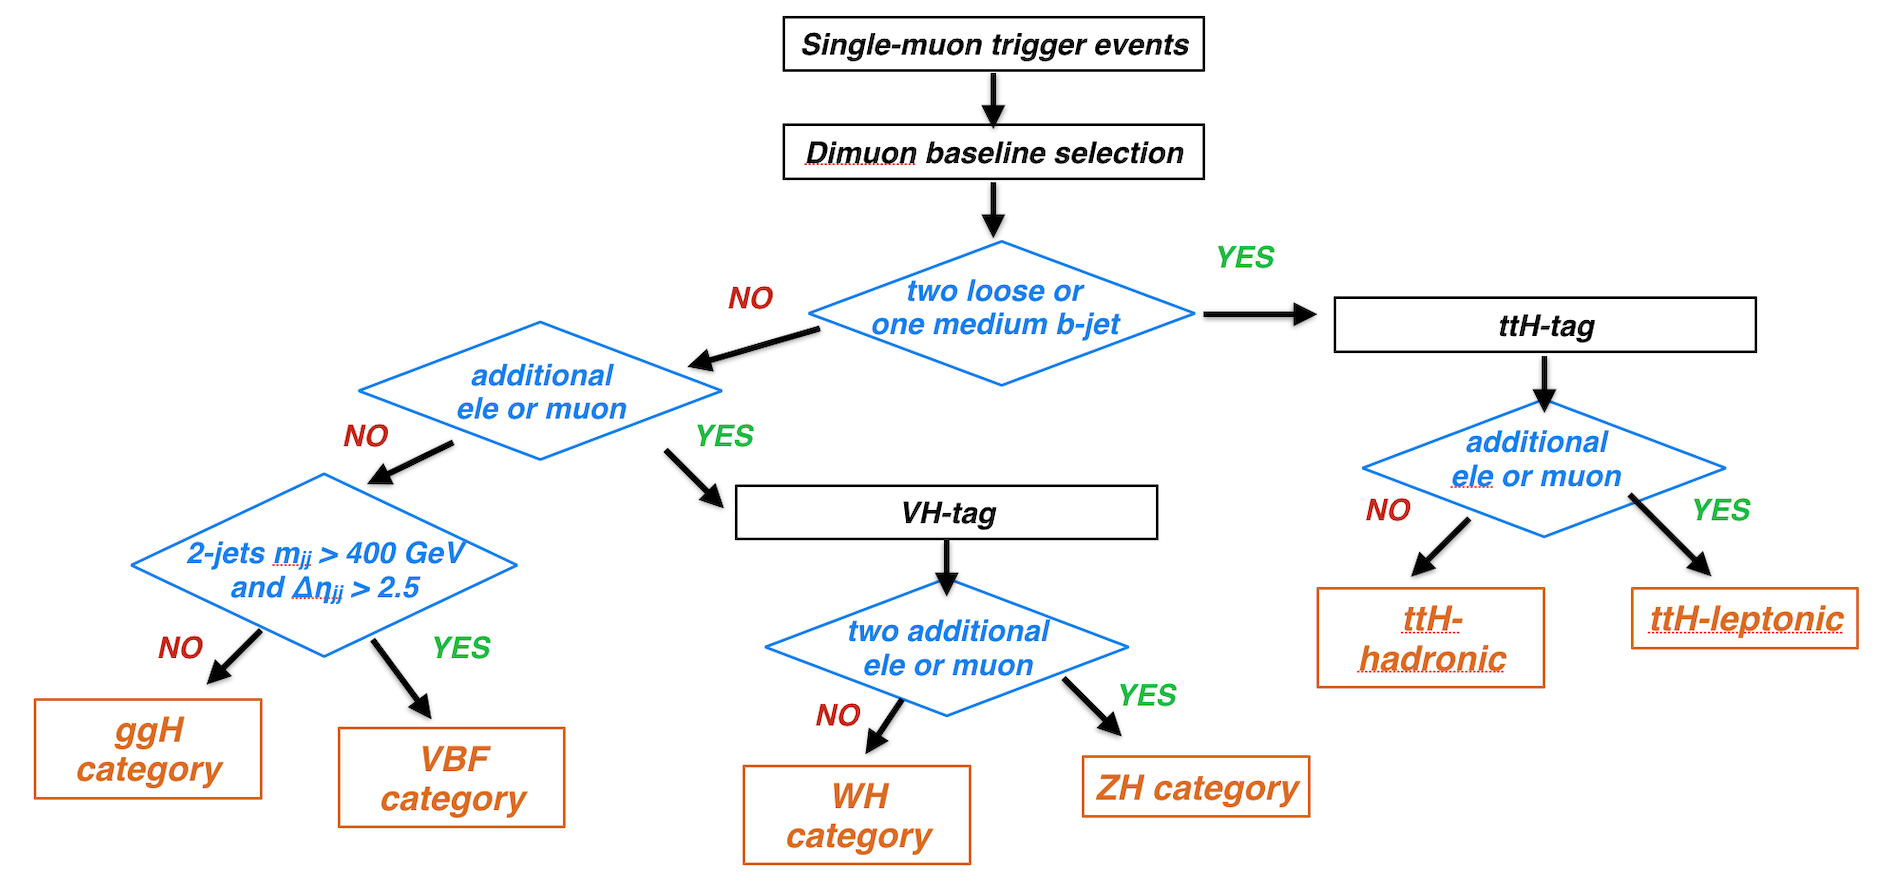
\includegraphics[width=0.9\textwidth]{pics/category_scheme.png}
    \caption{Scheme of the procedure of assigning events to different categories. All events passing the common baseline selection
             are divided into four mutually exclusive categories: \ggH, \qqH, \VH (\WH and \ZH), and \ttH (leptonic and hadronic).}
    \label{fig:event_categories}
\end{figure}

These categories have distinct profiles in expected signal yield, signal purity, and background composition.
Therefore the optimal analysis strategies are different.
Two strategies are considered for these categories:

\begin{itemize}
    \item \textbf{Data-driven parametric fit to the \mmm spectrum:} 
          As is done in the previously published analyses on the the data collected prior to 2017~\cite{2015184, PhysRevLett.122.021801},  
          a multivariate analysis (MVA) method is used to profile the separation between the signal and the background processes. 
          The MVA can be either cut-based as in the Run 1 analysis~\cite{2015184}, or machine learning (ML) based as in the analysis on the 2016 data~\cite{PhysRevLett.122.021801}.
          The MVA considers the kinematic information that is uncorrelated with the \mmm, and is used to divide the events into several regions 
          with different \SoB, called the MVA-categories. 
          In each MVA-category, the signal strength is evaluated from fits to the \mmm spectrum in data, in what is called the \textit{signal fit region}, for example $110<\mmm<150~\GeV$.
          Both the signal and the background are modeled by parametric functions that are carefully studied to provide a truthful description of the distributions of physics processes. 
          The total yield of the background is unconstrained in the fit and is determined entirely by the data.
          The effects of the systematic uncertainties from various sources on either the signal yield or the signal shape are assessed and propagated to the fit result. 
          The systematic uncertainties do not affect the background estimation since it is based on data rather than predictions from simulations.
    \item \textbf{MC-based template fit to the Neural Network discriminator:}
          This approach is also based on an MVA, for which a ML algorithm, Deep Neural Network (DNN), is taken.
          The DNN takes all the kinematic variables \textit{including \mmm}, and profiles the discrimination between the signal and the background.
          Without making further categories, the binned template of the DNN output in the whole phase space is used for the signal strength evaluation.
          Since the fit is applied to the DNN output rather than the \mmm distribution, the \textit{signal fit region} is further divided into two parts:
          the \textit{signal region}, $115<\mmm<135 ~\GeV$, and the \textit{sideband region}, $110<\mmm<115 ~\GeV$ or $135<\mmm<150 ~\GeV$.
          The data are fit simultaneously in both regions using the DNN templates of the signal and background simulation. 
          The systematic uncertainties affect both the signal and the background prediction, and are employed as variations in either the yield or the shape of the templates.
          The background yield is estimated from simulation and is allowed to vary within its uncertainty in the fit, in the same manner as the other systematic uncertainties.
          The signal strength is extracted from the fit in the \textit{signal region}.
          The \textit{sideband region} does not contain any signal contribution, but is nonetheless used in the fit, to enhance the constraint on the background estimation.
\end{itemize}

These two strategies should give comparable results in the ideal case, where there are abundant statistics in both data and simulation,
and where the data are well described by simulation.
However these conditions are usually not met in real analyses, and one strategy becomes preferable.
In scenarios where simulations do not model data very well, or where the uncertainties from simulations are not much smaller than the statistical uncertainty in data,
it is more advantageous to follow the data-driven approach.
In contrast, if an analysis lacks enough statistics in data but has abundant simulations that model data well, 
it is more beneficial to perform a MC-based analysis.

The \ggH category contains the majority of \hmm events with a very low \SoB. 
The statistical uncertainty of data is smaller than the systematic uncertainties of the background prediction from simulations.
Therefore it takes the data-driven strategy.
The \qqH category has a good amount of events, although much less than the \ggH category, and a good \SoB.
This makes it possible to pick very high \SoB regions with the help of MVA discriminators. 
The \qqH analysis prefers the MC-based strategy as there may be too few events in the high \SoB regions for a data-driven analysis.
The \VH and \ttH categories both have very few events, but high \SoB, which seem like good playgrounds for the MC-based approach.
However, the main backgrounds in the \VH and \ttH categories involve extra lepton(s) from nonprompt sources, which lacks accurate simulation estimates.
Moreover, the \VH and \ttH categories have less sensitivity than the \ggH and \qqH categories.
Adopting the MC-based approach in the \VH and \ttH categories would take a lot of computation resources and lead to insignificant improvements to the overall result.
The data-driven approach is much more cost-effective in the \VH and \ttH categories.
Overall, the \ggH, \VH, and \ttH categories follow the data-driven strategy, while the \qqH category takes the MC-based approach.

This thesis is focused on the analysis in the \VH category, the procedures of which are detailed in Chapter~\ref{chp:VH_analysis}.
The summary of all categories is reported in Ref.~\cite{Sirunyan_2021}.
Chapter~\ref{chp:hmm_results} describes the results of the \VH analysis and the combined results of all four categories.

\chapter{Object reconstruction and identification}\label{chp:objects}

\section{CMS object reconstruction}

\section{Object selectoin in the H to muons analysis}
\chapter{Muon momentum correction and calibration} \label{chp:muon_corr}

This analysis aims to find a sharp signal peak on top of a smooth background in the \mmm distribution.
It is of crucial importance to correct any mismeasurement in the muon momentum scale 
and to remove any momentum dependence on variables like $\eta$ and $\phi$ of muons.
It is also crucial to minimize the momentum and resolution differences between data and simulation, 
so that there is no significant bias in the signal modeling.

Three sets of corrections are applied in this analysis: 
the \RochCorr~\cite{Bodek:2012id}, the recovery of the final-state radiation (FSR) photons, and the \GeoFit.
The \RochCorr is a centrally provided correction (by CMS), which corrects 
the biases in the muon momentum resulted from the mismodeling of detector alignment and magnetic field. 
A brief description of the \RochCorr is given in Section~\ref{sec:Roch_corr}, 
while the technical details can be found in the Ref.~\cite{Bodek:2012id}.
The \FSR is a common practice in many CMS analyses, which corrects the muon energy loss via FSR.
The recovery scheme in this analysis is optimized specifically for the \hmm decay, which is described in Section~\ref{sec:fsr} and in more detail in Ref.~\cite{oliverthesis}.
The \GeoFit is developed by the author in the context of the \hmm analysis and approved by the CMS collaboration.
It uses information of muon vertexing to correct the biases in muon momentum of the reconstructed muon tracks.
The development of the \GeoFit is described in details in Section~\ref{sec:GeoFit}.
The effects of the three corrections are orthogonal.
In practice, the \RochCorr is applied to all muons, then each muon is surveyed for FSR photons.
If an FSR photon is found associated to the muon, the \FSR is applied, 
if not, the \GeoFit is applied.\footnote{The performance of \GeoFit on muons with FSR is not validated and maybe suboptimal. 
Furthermore, as FSR muons are a small fraction, the difference whether to apply \GeoFit to them is negligible.}

These three corrections are applied to both data and simulation.
The performance of the corrections is examined with the study on the \zmm peak,
which is listed in details in Section~\ref{sec:muon_cal}.
These corrections fix all the known biases in muon measurement, 
and ensure a per-mille-level agreement between data and simulation. 

\section{Rochester correction} \label{sec:Roch_corr}

In reality, the CMS detector can have various imperfections, 
such as the misalignment of the detector components, and the uncertainties in the magnetic field.
Sometimes these imperfections are not correctly emulated in reconstruction softwares, 
and as a result, the reconstructed muons can be inaccurate.
These inaccuracies are reflected as the dependences of the muon momentum on its \eta, \phi ~coordinates, and its charge.

On the other hand, in the simulation of CMS events, none of the imperfections are assumed,
which leads to slightly different detector responses from those in data, and in turn over-optimistic modelings in the muon measurement. 
Therefore the correction for simulation and for data have to be different.
The generated muon information, smeared with some functional forms to match the experimental resolution, 
is used as the reference for both data and simulation. 

The well-understood \zmm events are used to develop the \RochCorr. 
The idea of the correction is briefly summarized as follows:
\begin{itemize}
  \item For data, reconstructed simulation (reco-sim), and the reference simulation (ref-sim), 
        muons are divided into different \eta ~and \phi ~bins, separately for $\mu^{+}$ and $\mu^{-}$.
        In each bin, the $1/\pt$ distributions of data and reco-sim are corrected so that the mean value of the distribution becomes the same as that in the ref-sim.
  \item The $1/\pt$ distribution in reco-sim is usually narrower than that in data. 
        A smearing is applied to the reco-sim $1/\pt$ distribution so that it matches the resolution in data.
  \item After the steps above, the \mmm in each bin may still be off from the expected distribution by some small amounts.
        The ratio between this offset and the nominal \PZ mass is applied to the muon \pt as a correction factor iteratively, until the offset is minimized.
\end{itemize}
The \RochCorr removes the dependences of \mmm on muon \eta,~ \phi,~ and charge, 
as well as the \mmm resolution differences between data and the simulation.
Details of the performance of the \RochCorr can be found in Section~\ref{sec:muon_cal}.


\section{FSR recovery} \label{sec:fsr}

In CMS, muons produced in $pp$ collisions may radiate photons and lose energy, which is referred to as the final-state radiation (FSR).
The radiation may carry substantial energy and lead to an underestimation of the original muon momentum.
This leads to two effects in this analysis:
a loss of event acceptance, and a smearing of the \mmm resolution.
This can be mitigated by identifying some of the FSR photons adding their energy back to the muon energy, called the \FSR.

The selection for the FSR photons is modified on top of the strategy developed in the CMS $\PH \to \PZ\PZ$ analyses~\cite{Sirunyan:2017exp, Sirunyan:2018qlb}.
The selection criteria is summarized as follows:
\begin{itemize}
  \item Photons with transverse energy $E^{\gamma}_{T} > $ 2 \GeV and $|\eta|<1.4$, $1.6<|\eta|<2.4$ are considered as FSR candidates.
  \item The photon is required to be within the cone of $\Delta{}R<0.5$ around its closest muon that satisfies $\pt >$ 20 \GeV and $|\eta| < 2.4$.
  \item The photon is not identified as a bremsstrahlung photon associated with a reconstructed electron.
  \item The PF isolation of the photon in a cone of $\Delta{}R < 0.3$ should be less than 1.8, i.e. $\sum_{i}\pt^{i}(\Delta{}R(\gamma, i)<0.3)/\pt(\gamma) < 1.8$, 
        where $i$ iterates the PF objects around the photon other than the candidate muon.
  \item The separation between the photon and the muon satisfies $\Delta{}R(\mu, \gamma)/\pt^{2}(\gamma) < 0.012$.
  \item In order to suppress energetic photons from the $\PH \to \PZ\gamma \to \mu\mu\gamma$ process,
        the \pt ratio between the photon and the muon is required to be less than 0.4, i.e. $\pt(\gamma)/\pt(\mu) < 0.4$.
  \item If multiple FSR photons are associated to the same muon, only the photon with the smallest $\Delta{}R(\mu, \gamma)/\pt^{2}(\gamma)$ is taken.
\end{itemize}

With this set of selection, about 3\% of signal events are tagged with FSR photons.
The selection is also very effective in reducing the $\PH \to \PZ\gamma$ events,
whose final yield is about 0.1\% of the overall \hmm signal and can be neglected.
The momentum of the FSR photons are added to the muon momentum, 
while the photons themselves are removed from the calculation of the muon isolation.
The \FSR significantly improves the \mmm reconstruction in the FSR tagged events, as shown in the left plot of Figure~\ref{fig:fsr_sig}.
The overall effect on the inclusive signal, as shown in the right plot of Figure~\ref{fig:fsr_sig}, 
is a 3\% improvement on the \mmm resolution and a 1.7\% increase in the total signal yield. 
The \FSR is applied in all categories of the \hmm analysis and resulting improvement on the combined significance is about 3\%.
The performance of \FSR is also validated with the \zmm events, shown in Figure~\ref{fig:fsr_val},
where a good agreement is kept between simulation and data with or without the \FSR. 
The \FSR is expected to perform the same way on data as on simulation, 
and no bias is introduced by the application of the \FSR. 

\begin{figure*}[!htb]
      \centering
      \captionsetup{justification=justified}
      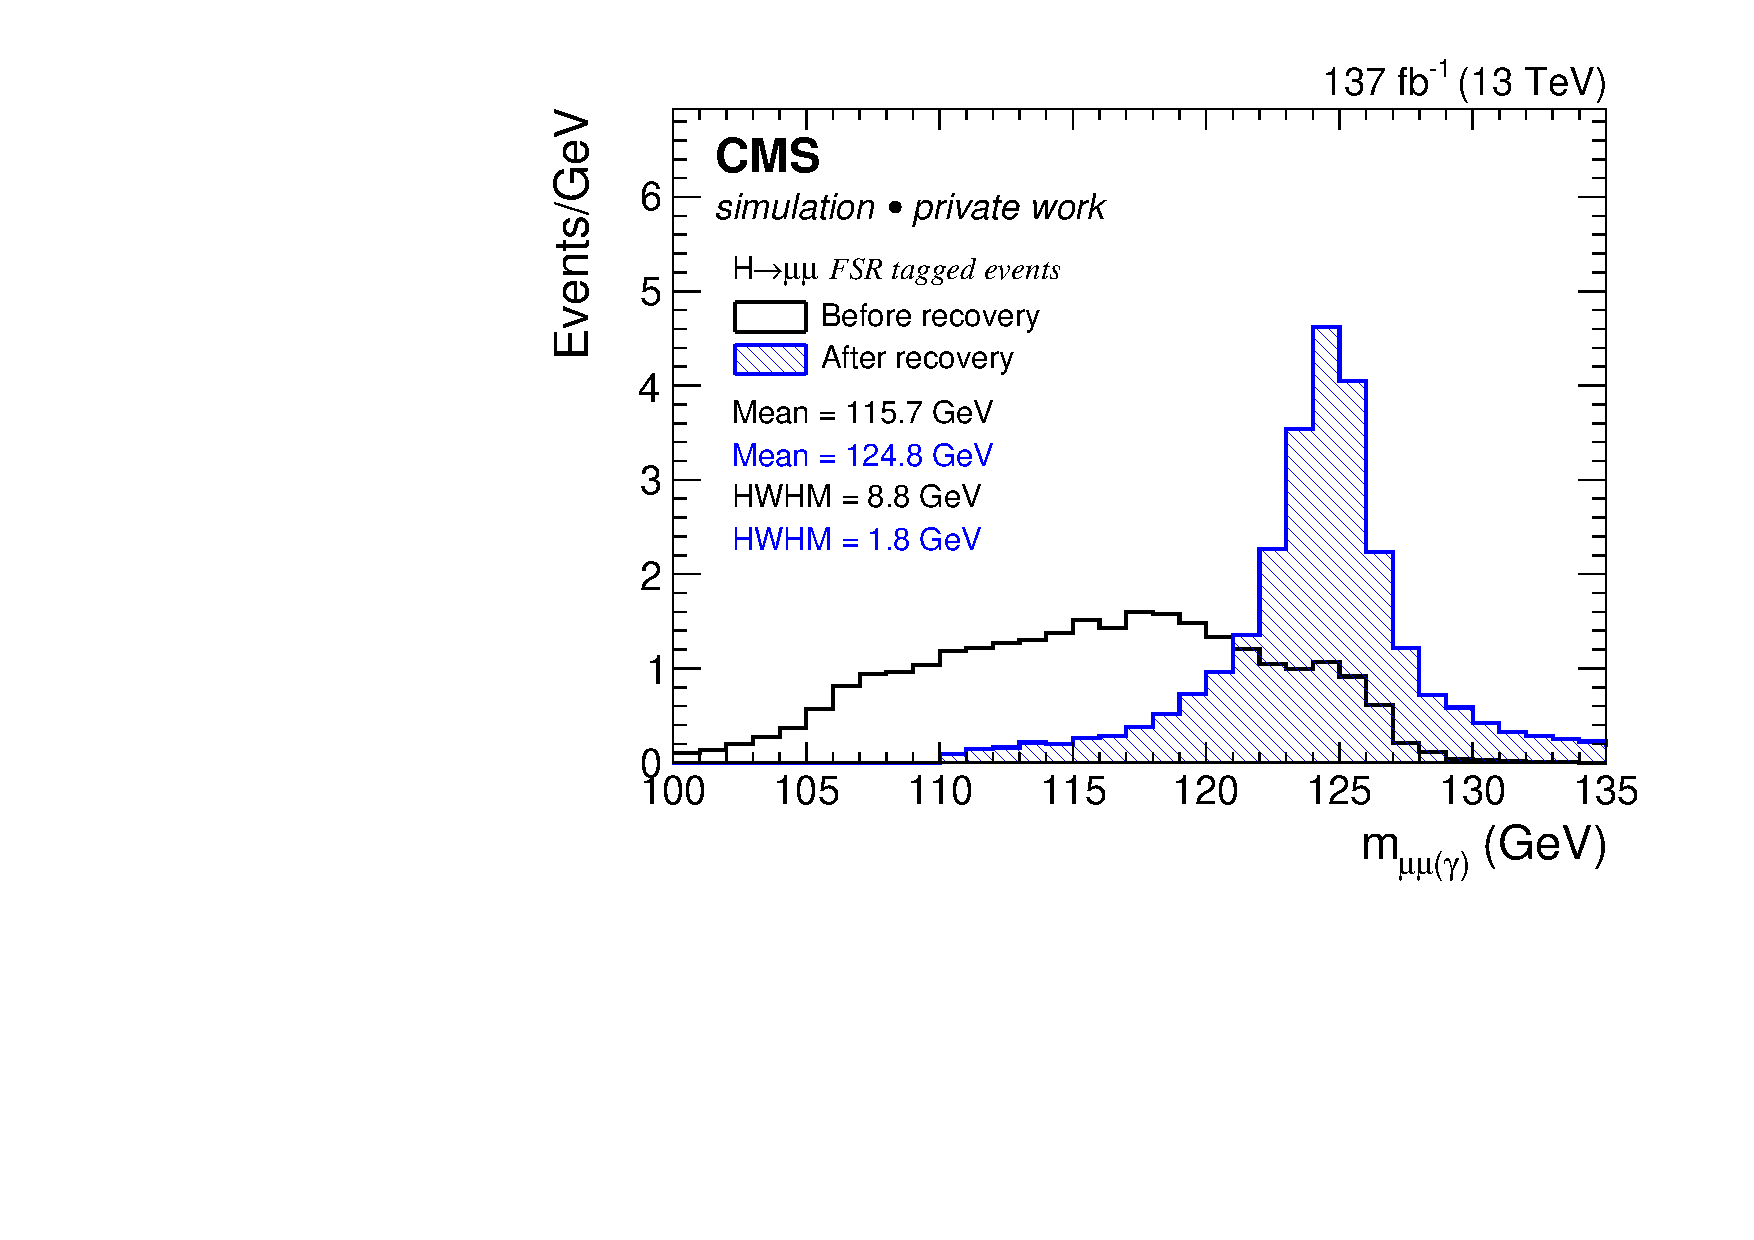
\includegraphics[width=0.45\textwidth]{pics/muon_corr/FSR/FSRrecovery_FSRtagged.pdf}
      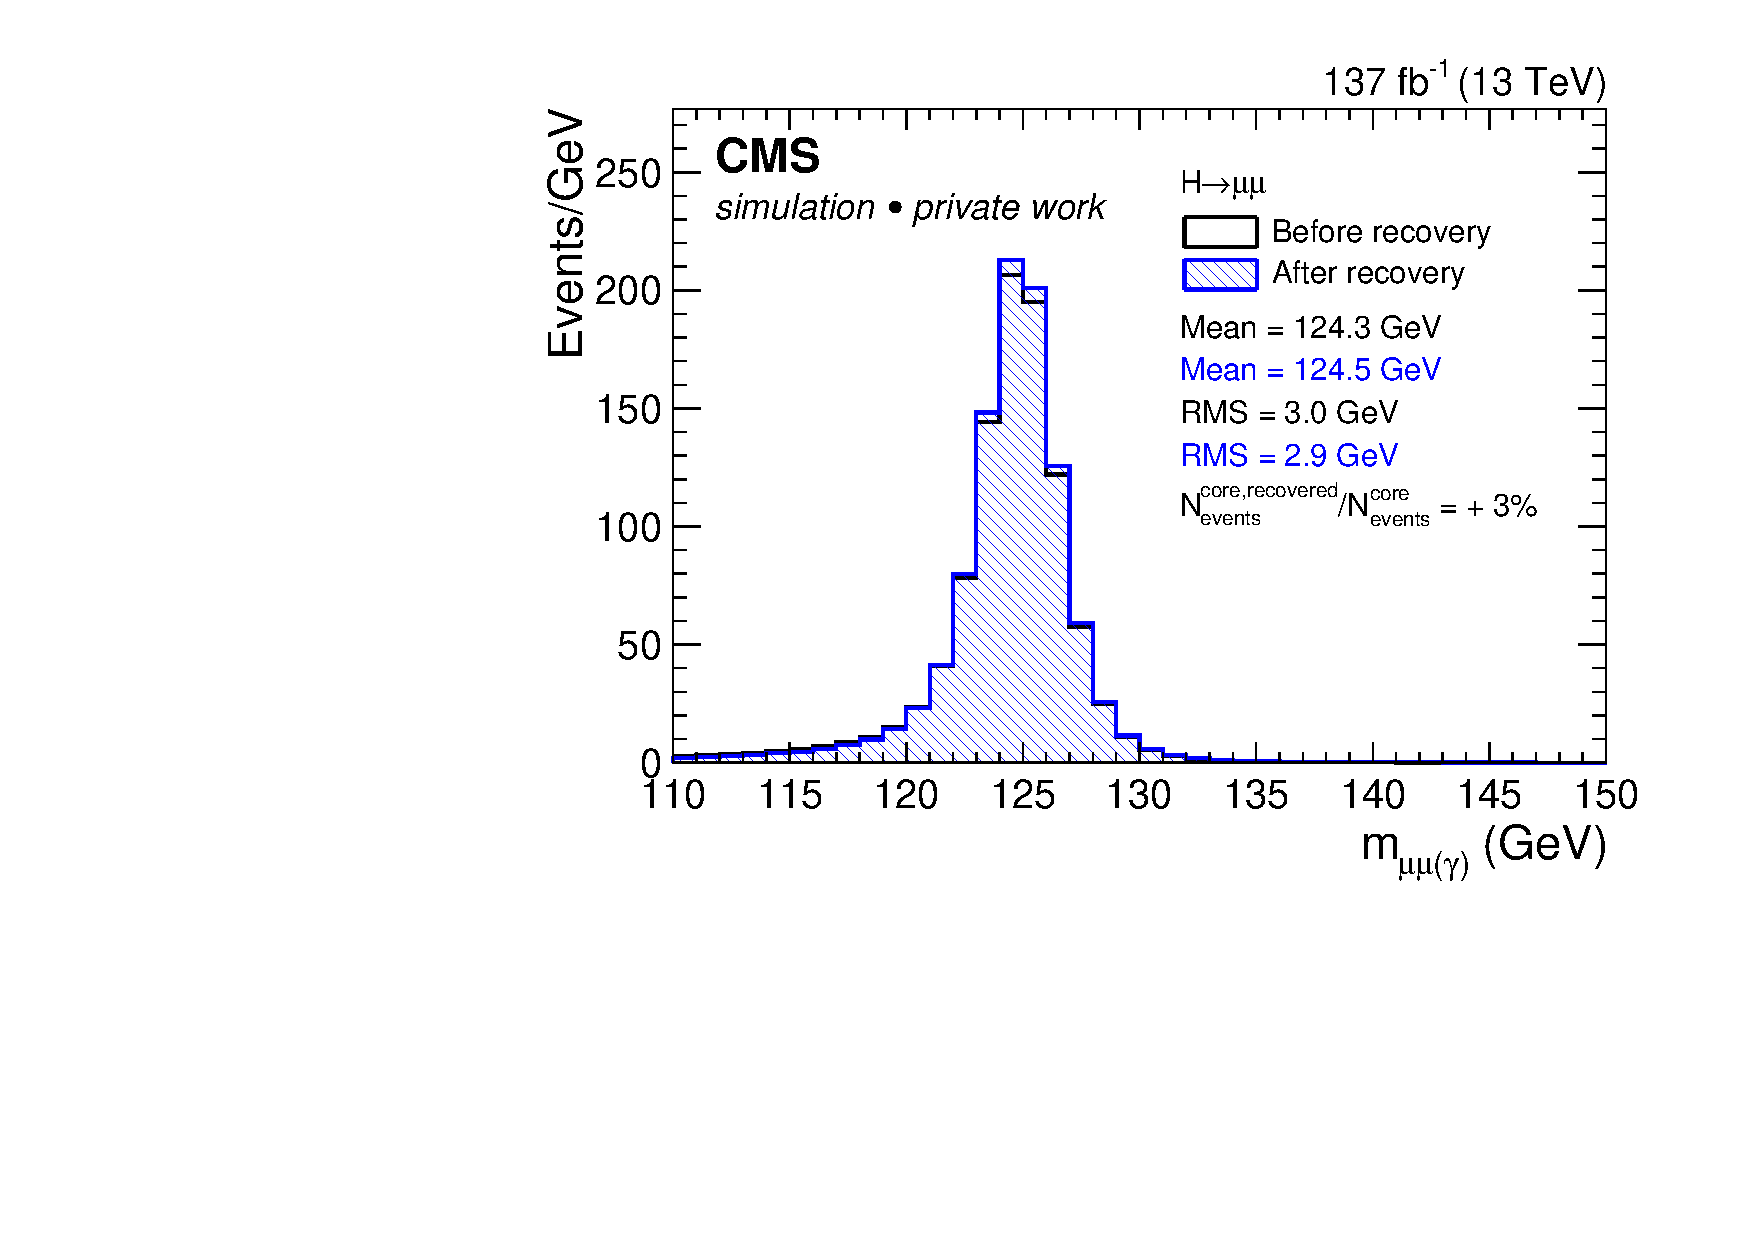
\includegraphics[width=0.45\textwidth]{pics/muon_corr/FSR/FSRrecovery_FullSignal.pdf}
      \caption{Performance of the \FSR in the simulated \hmm events. 
               The \mmm before and after the \FSR are shown for the events that contain at least one FSR photon (left),
               and for the inclusive signal events (right).
               Plot taken from Ref.~\cite{oliverthesis}.}
      \label{fig:fsr_sig}
\end{figure*}

\begin{figure*}[!htb]
      \centering
      \captionsetup{justification=justified}
      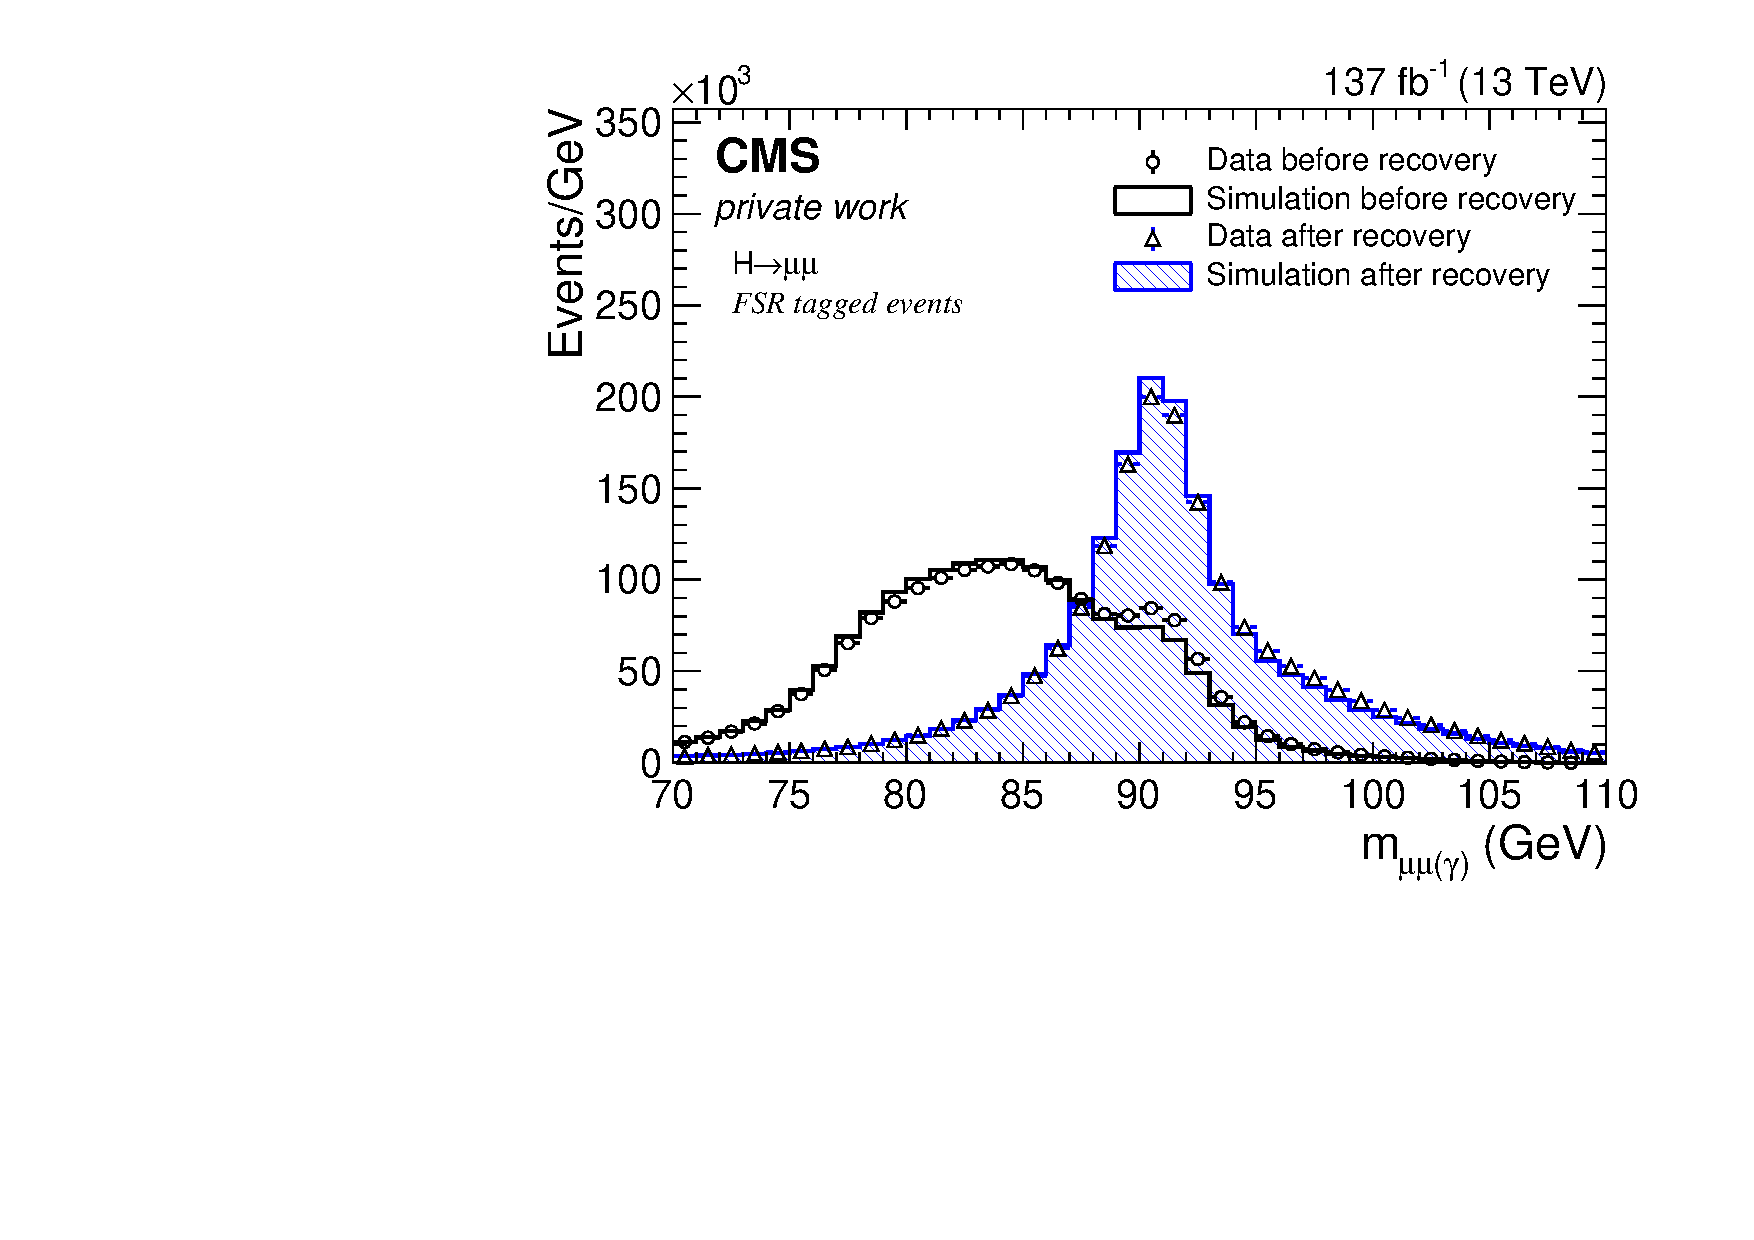
\includegraphics[width=0.45\textwidth]{pics/muon_corr/FSR/FSRrecovery_Validation.pdf}
      \caption{Performance of the \FSR in the \zmm events that contain FSR photons, in both data and simulation. 
               A good agreement between simulation and data is observed, both before and after the correction.
               Plot taken from Ref.~\cite{oliverthesis}.}
      \label{fig:fsr_val}
\end{figure*}


\section{GeoFit correction} \label{sec:GeoFit}

As described in Section~\ref{sec:reco_track},
tracks are built from hits in silicon trackers and extrapolated to the collision region
without any assumption on their vertices.
Reconstructed tracks may have nonzero displacements from their true origins because of uncertainties in track fits.
If there is a way to locate the true origin of a track, 
it can be used as a constraint on the track to improve the track momentum measurement.
Prompt tracks originate from $pp$ interaction points, 
which are estimated by primary vertices (PV, Section~\ref{sec:reco_pv}) or the beamspot (BS, Section~\ref{sec:reco_bs}).
This section reports the development of a momentum correction for prompt muons (the \GeoFit)
by taking the PV or BS as their true origins.

This correction is based on a geometrical correlation between the \pt mismeasurement 
and the displacement from the reconstructed track to its true vertex.
The correction is applied as a simple analytic function whose parameters are determined from fits to simulations.
It is therefore named the \GeoFit.
Section~\ref{sec:d0_geometry} explains the geometry of the track displacement and the correlation between different variables.
Section~\ref{sec:dev_geofit} describes the studies on simulated samples to find the best fit parameters in that correlation.
The \GeoFit is developed using muon tracks from the $\PZ \to \mu\mu$ process.
It removes the dependence of \mmm on track displacement, which leads to an 
improvement on the \mmm resolution of the combined signal ranging from 3\% to 10\%, depending on the data-taking period.
Details of the \GeoFit performance, along with validation studies are shown in Section~\ref{sec:perf_geofit}.
In addition, an alternative way to correct this \pt bias is to redo the track fit including the colliding vertex as an additional hit in the track, 
which should achieve a more fundamental correction at the cost of more computational resources.
A preliminary study comparing the \GeoFit with the track refit shows the two methods give almost equivalent results,
detailed in Section~\ref{sec:track_refit}.


\subsection{Geometry of the track displacement}\label{sec:d0_geometry}

The displacement of a track from a vertex is usually measured as the impact parameters, $d_{xy}$ and $d_{z}$,
which are the signed distances between the vertex and its point of closest approach (PCA) to the track, in the transverse and longitudinal directions.
In CMS, because most studies only care about the transverse impact parameter, 
the PCA is defined as the point on the 2D-projection of the track in the transverse plane that is the closest to the vertex.
Note that the PCA of the 2D-track is not necessarily the 2D-projection of the PCA in the 3D-space. 
The $d_{z}$ is calculated at the 3D-point corresponding to the 2D-PCA, rather than the 3D-PCA.
As the $d_{z}$ is not used in our studies, the term "impact parameter", if not otherwise stated,
refers specifically to the transverse impact parameter $d_{xy}$, also denoted as $d_{0}$.
The definition of $d_0$ can be expressed as 
\begin{equation}\label{eq:d0_def}
  d_0 = -x_{0} \cdot \text{sin}(\phi_{0}) + y_{0} \cdot \text{cos}(\phi_{0})
\end{equation}
where $(x_{0}, y_{0})$ is the coordinate of a point near the vertex in the frame, in which the vertex is at $(0,0)$, 
and $\phi_{0}$ is the azimuthal angle of the track at $(x_{0}, y_{0})$.
A scheme for this definition is shown in Figure~\ref{fig:d0_def}.

\begin{figure*}[!htb]
      \centering
      \captionsetup{justification=justified}
      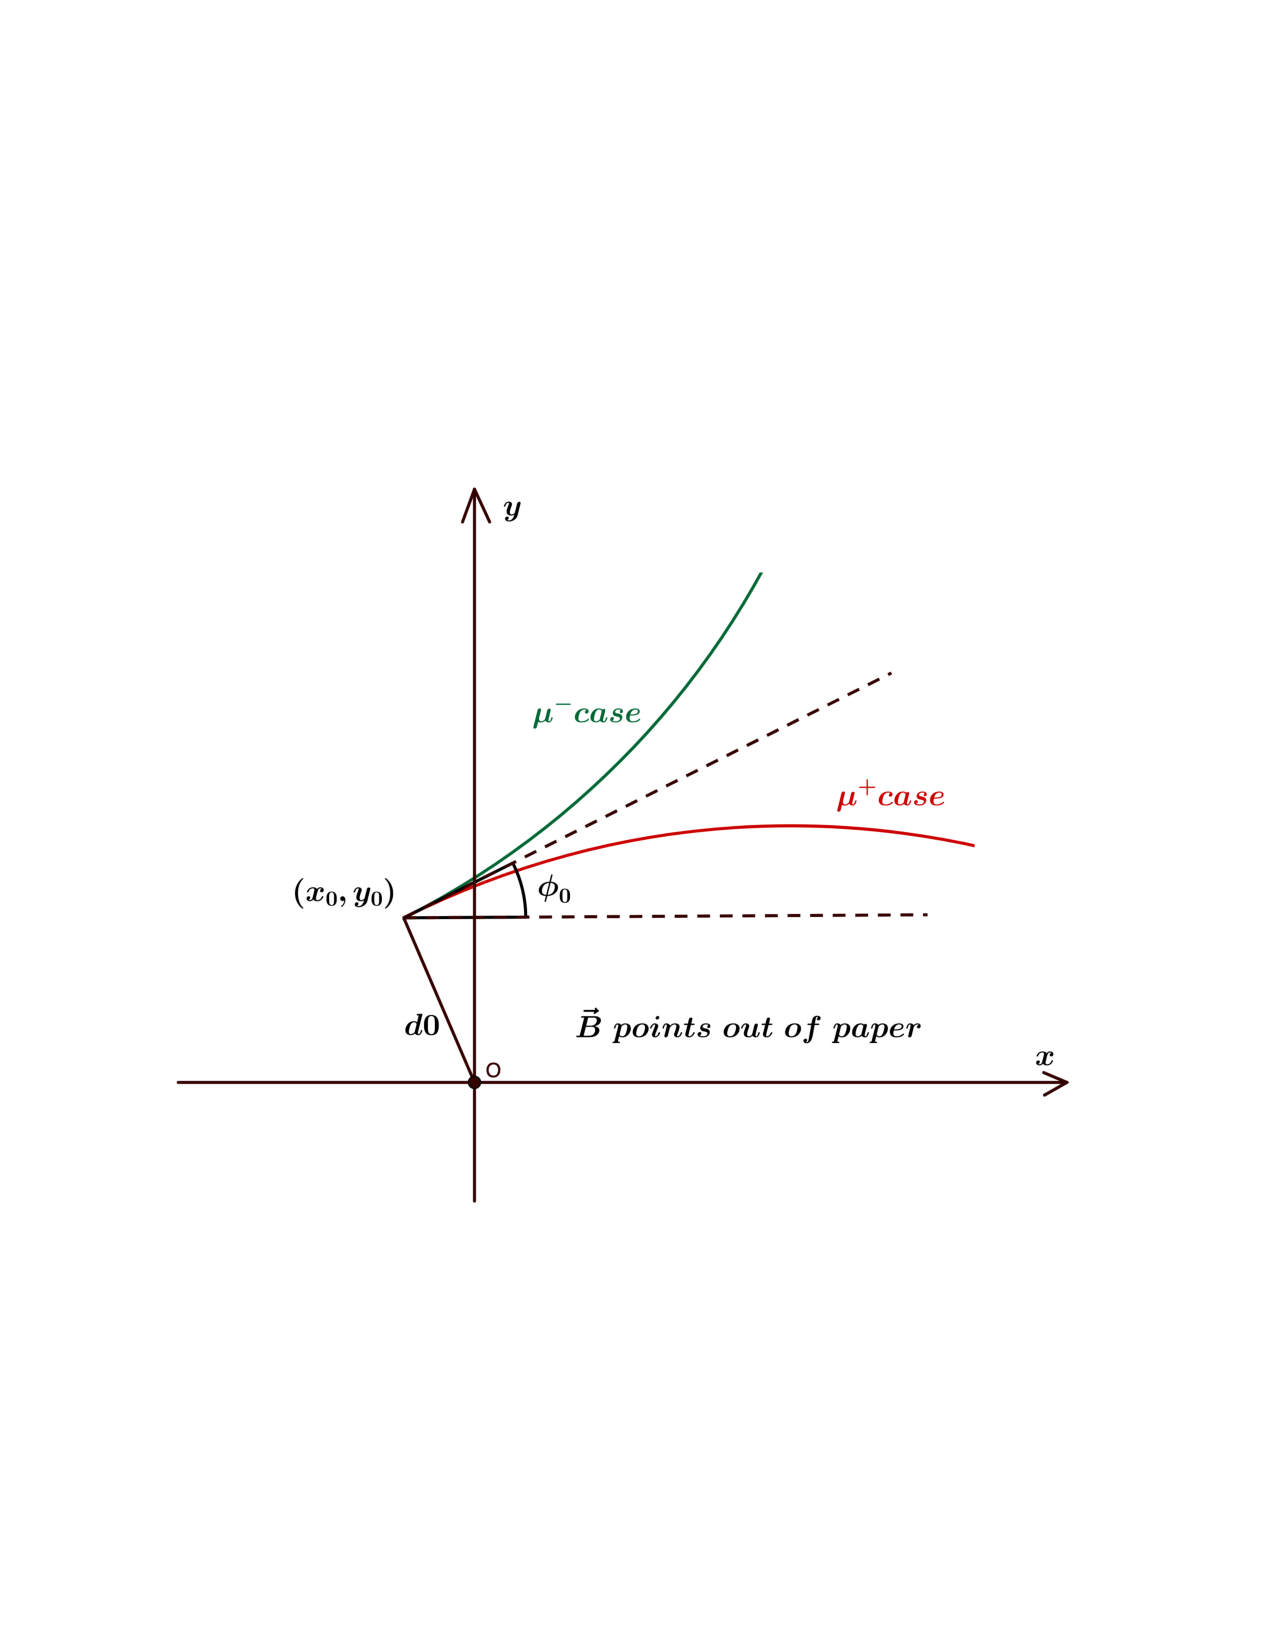
\includegraphics[width=0.70\textwidth]{pics/muon_corr/GeoFit/d0_def.pdf}
      \caption{Scheme of the $d_0$ definition in CMS. The $(x_{0}, y_{0})$ is the coordinate of 
               a point near the vertex in the frame where the vertex is at $(0,0)$, 
               and the $\phi_{0}$ is the azimuthal angle of the track at $(x_{0}, y_{0})$.}
      \label{fig:d0_def}
\end{figure*}

\begin{figure*}[!htb]
      \centering
      \captionsetup{justification=justified}
      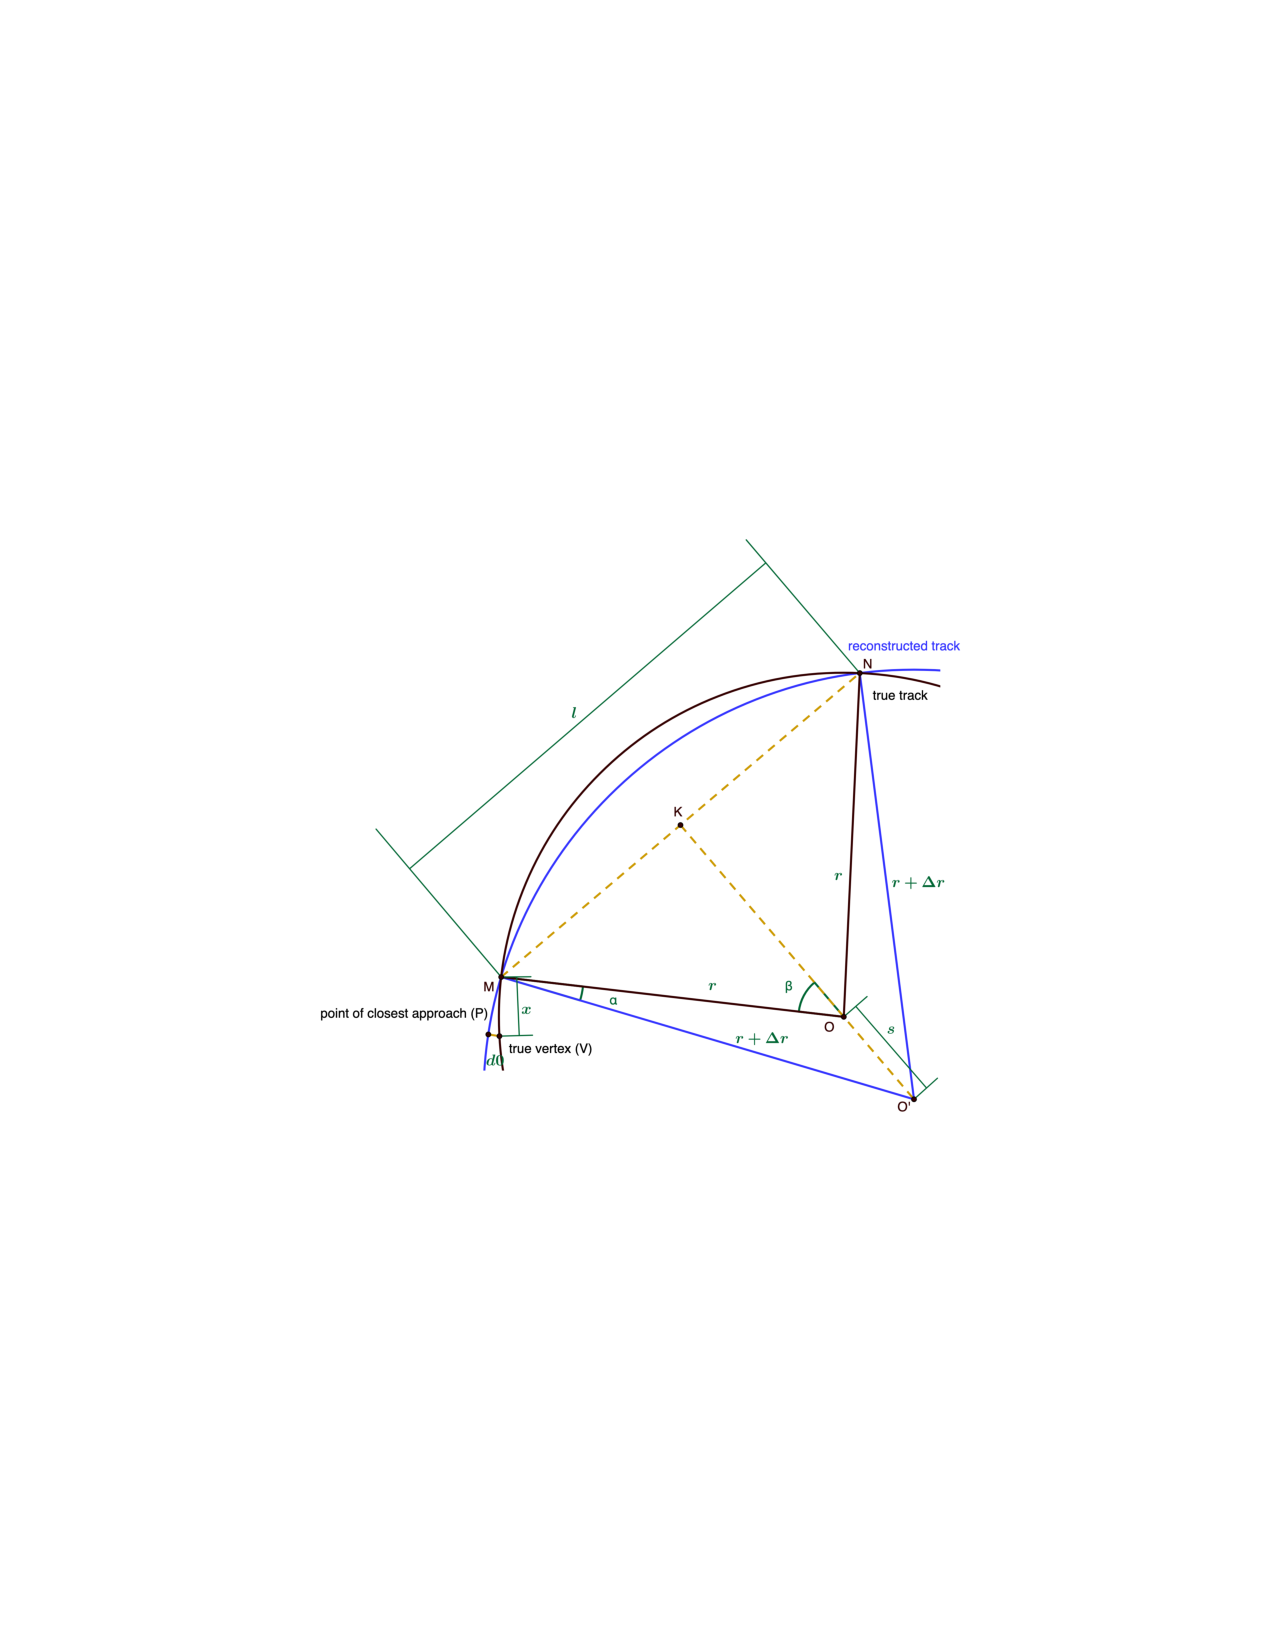
\includegraphics[width=\textwidth]{pics/muon_corr/GeoFit/d0_pt_geometry.pdf}
      \caption{Scheme of the track geometry in the transverse plane. 
               The blue lines show the geometry of the reconstructed track, 
               compared to the black lines, which are the geometry of the true track.
               The difference between the blue track and black track is exaggerated in this scheme.
               The blue track and the black track must intersect at two points.
               $l$ is the distance between the two intersections, 
               and $x$ is the distance between the true vertex and the first intersection.
               $s$ is the distance between the circular centers of the two tracks.}
      \label{fig:d0_pt_scheme}
\end{figure*}

In the track geometry, illustrated in Figure~\ref{fig:d0_pt_scheme}, 
the reconstructed track is very close to, but slightly deviated from, the true track,
which leads to a small $d_0$ between the reco track and the true vertex, 
as well as a small distance between the circular centers of the reco track and the true track.
The circular centers of the two tracks are labels as $O$ and $O'$ for the true track and the reconstructed track,
and $s$ is the distance between $O$ and $O'$. 
The radii of the two tracks are $r$ and $r'$, with $\Delta{}r = r' - r$.
The two circles must intersect at two points, labeled as point $M$ and $N$, 
with the distance between $M$ and $N$ denoted as $l$.
$\beta$ is half of the central angle spanned by the chord $l$ in the true track,
while $\alpha$ is the angle $\angle O'MO$.
The true vertex is denoted as $V$, with $d_0$ as the impact parameter of the reco track to it,
while the PCA on the reco track is denoted as $P$.
The distance between $M$ and $V$ is marked as $x$.
As this scheme represents typical muon tracks in CMS, 
the radii of the tracks under study are at the scale of several tens of meters,
and the $\Delta{}r$ is expected to be much smaller than $r$.
Points $M$ and $N$ are expected to be around the coverage of the CMS tracker system, which is about a meter.
Therefore $x$ and $l$ are expected to be much smaller than $r$ as well.
Finally, the $d_0$ scale of the tracks under study is about ten microns, which is much smaller than $x$, $l$, and $r$. 

In this setup, a few geometrical relationships can be found between different variables, listed as follows:
Since $x \ll r$, arc $\stackrel{\frown}{VM}$ and $\stackrel{\frown}{PM}$ can be viewed as line segments which are respectively perpendicular to $OM$ and $O'M$.
Therefore in triangle $\triangle VMP$, 
\begin{equation}\label{eq:d01}
      d_0 = x \cdot \text{sin}\alpha
\end{equation}      
In triangle $\triangle O'MO$, the sine law gives
\begin{equation}\label{eq:d02}
      \frac{s}{\text{sin}\alpha} = \frac{r+\Delta{}r}{\text{sin}\beta}
\end{equation}
And in triangle $\triangle OMK$, 
\begin{equation}\label{eq:d03}
      \text{sin}\beta = \frac{l/2}{r}
\end{equation}   
Then, using the Pythagorean theorem in both triangle $\triangle O'MK$ and triangle $\triangle OMK$, there is
\begin{equation}\label{eq:d04}
      s =  \sqrt{(r+\Delta{}r)^{2} - (l/2)^{2}} - \sqrt{r^{2} - (l/2)^{2}}
\end{equation}   
Combining Equation ~\ref{eq:d01} to ~\ref{eq:d04} and assuming $r \gg l$, one can get
\begin{equation}\label{eq:d05}
      d_0 = \frac{xl}{2} \cdot \frac{\Delta{}r}{r^{2}}
\end{equation}  
Note that in CMS, under the 3.8T magnetic field, tracks follow 
\begin{equation}
    \pt ~(\text{in ~\GeV}) = 1.14 \cdot r ~(~\text{in meter})   
\end{equation}
We reach
\begin{equation}\label{eq:d0_prop}
    d_0 \propto \frac{\Delta{}\pt}{\pt^{2}}
\end{equation}

Now a quantitative relationship is extracted between $d_0$ and \pt, but with one caveat:
the variables $x$ and $l$ in the scheme above may vary track by track, and are impossible to measure in real data,
meaning that the coefficient in the proportionality is not a constant for different tracks, and Equation~\ref{eq:d0_prop} can be smeared.
Therefore, to validate this proportionality, studies are performed on simulated samples comparing the reconstructed \pt and the generated \pt of muon tracks.
Plots of $(\pt^{reco}-\pt^{gen})/ (\pt^{gen})^{2}$ vs $d_0$ are made, 
to see whether the proportionality can be observed after the smearing,
which is the topic of Section~\ref{sec:dev_geofit}.

Another remark needs to be made, that in Figure~\ref{fig:d0_pt_scheme} the \pt mismeasurement is related to the relative position of the true vertex to the reconstructed track.
To be more specific, if the true vertex is inside of the reco track, the \pt is overestimated, 
while if the true vertex is outside of the reco track, the \pt is underestimated. 
However, in the CMS definition of $d_0$ shown in Figure~\ref{fig:d0_def}, the sign of $d_0$ corresponds to an opposite relative position between the vertex and the track
for the positively charged muons and the negatively charged muons. 
A positive $d_0$ value means the true vertex is inside of the reco track if the muon is positive, but outside of the reco track if the muon is negative.
Therefore in CMS convention the $d_0-\pt$ correlation is expected be reversed for different muon charges,
and in Section~\ref{sec:dev_geofit} studies are always performed evaluating $d_0 \times$ charge rather than just $d_0$.

\subsection{Development of GeoFit}\label{sec:dev_geofit}

The $(\pt^{reco}-\pt^{gen})/ (\pt^{gen})^{2}$ vs $d_0$ plots are made with the following steps:
The values $\pt^{reco}$, $\pt^{gen}$, and $d_0$ are extracted for each track in simulated samples.
The distribution of $(\pt^{reco}-\pt^{gen})/ (\pt^{gen})^{2}$ is made for tracks in different $d_0 \times$ charge bins.
The maximum position and the corresponding full-width-half-maximum (FWHM) is found for each 
fine-binned $(\pt^{reco}-\pt^{gen})/ (\pt^{gen})^{2}$ distribution and set as the value and the uncertainty
of one data point in the plots in Figure~\ref{fig:pv_vs_bs_fits}.
The plots are then fit with analytic functions, which are considered as the experimental realization of Equation~\ref{eq:d0_prop}.

In CMS, the colliding vertex is measured by two physics objects, 
the primary vertex (PV) and the beamspot (BS), as described in Sections~\ref{sec:reco_pv} and ~\ref{sec:reco_bs}.
Both vertex types are tested and compared in the development of \GeoFit.
Examples of the corresponding $(\pt^{reco}-\pt^{gen})/ (\pt^{gen})^{2}$ vs $d_0$ dependences are shown in Figure~\ref{fig:pv_vs_bs_fits}.
The dependence in the PV plot is not linear as the reconstructed PV is pulled towards the energetic muon tracks,
while the dependence in the BS plot follows a linear trend as predicted in Equation~\ref{eq:d0_def}.
This is understood as the PV position, reconstructed with a limited number of tracks, 
can be biased toward the few energetic tracks associated to it, 
while the BS, averaging numerous tracks from many events, is less affected by individual tracks.
Therefore the BS is considered as the position of the true vertex in the rest of the study.


\begin{figure*}[!htb]
      \centering
      \captionsetup{justification=justified}
      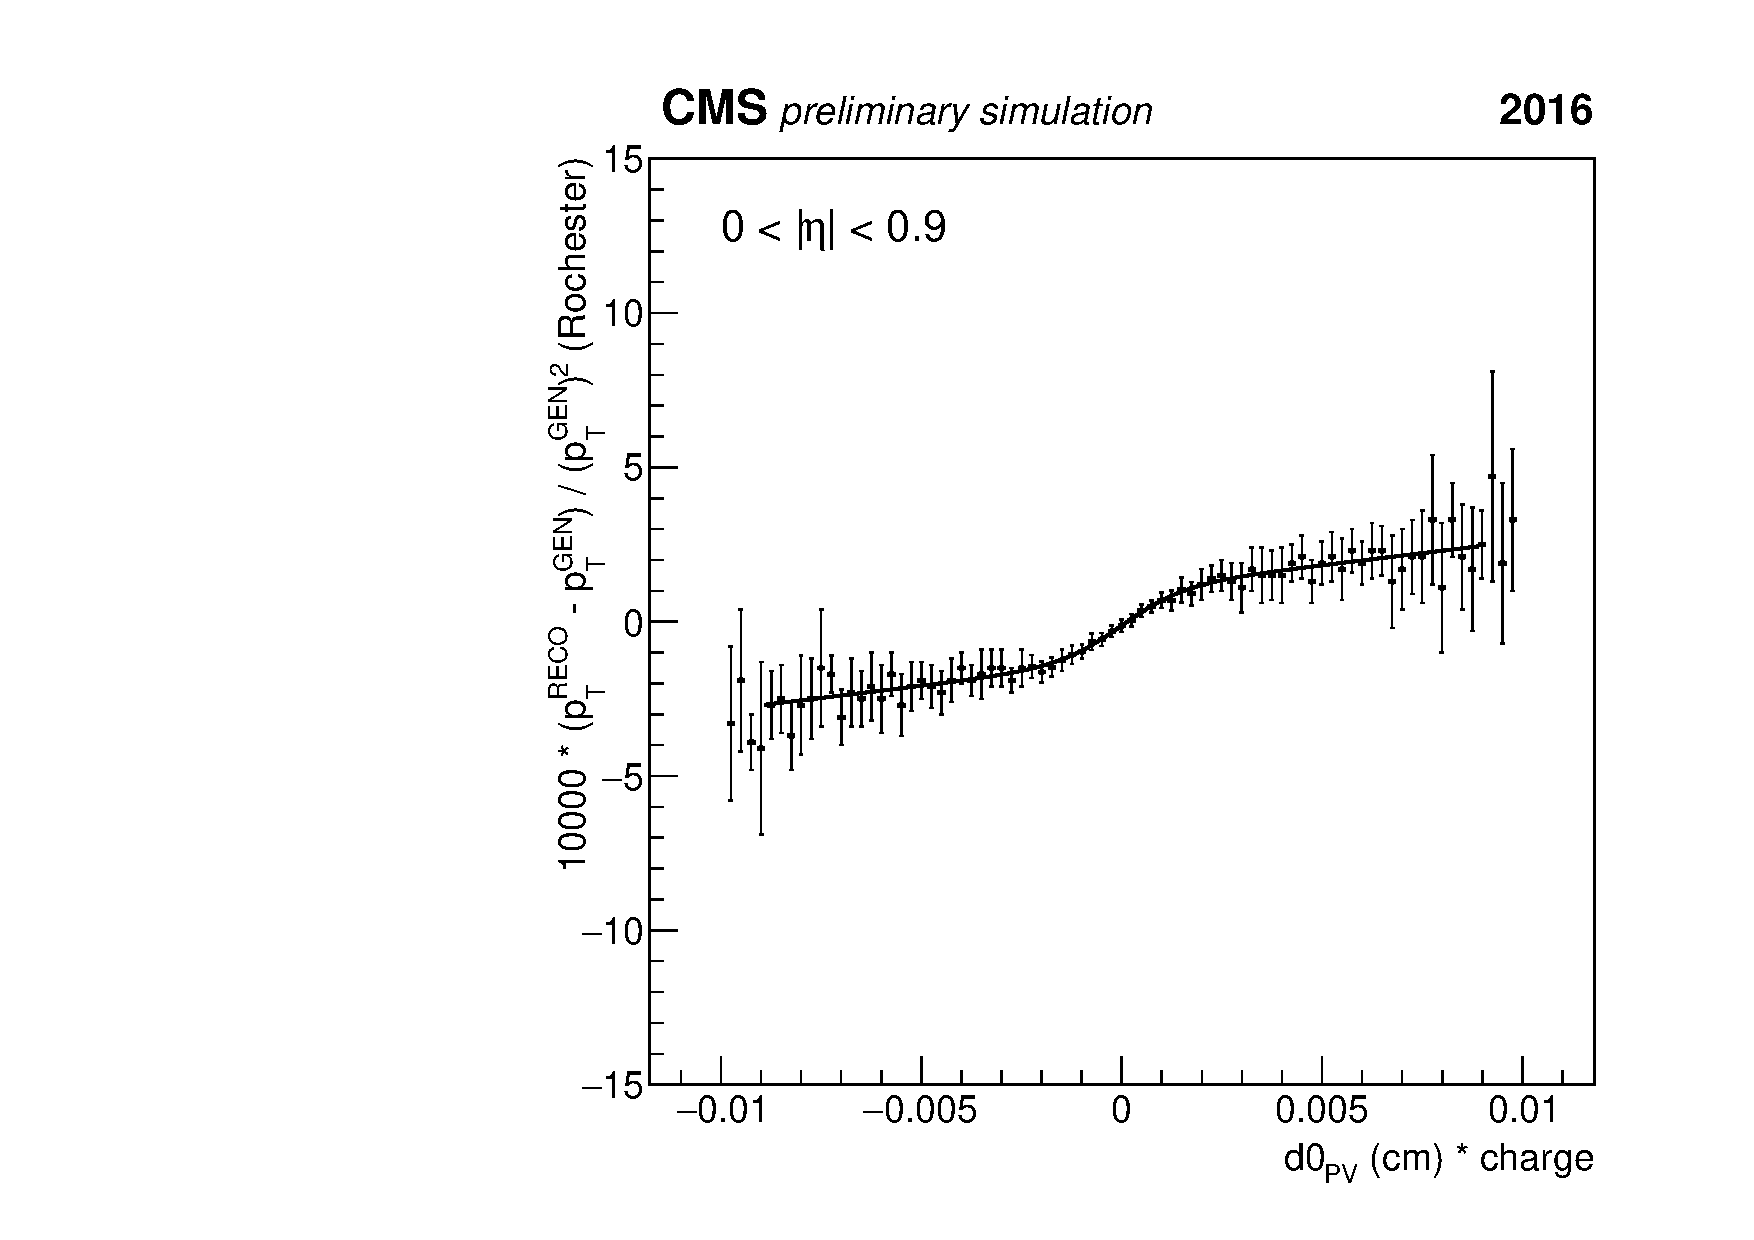
\includegraphics[width=0.45\textwidth]{pics/muon_corr/GeoFit/fit_results/d0_pt_PV_eg.pdf}
      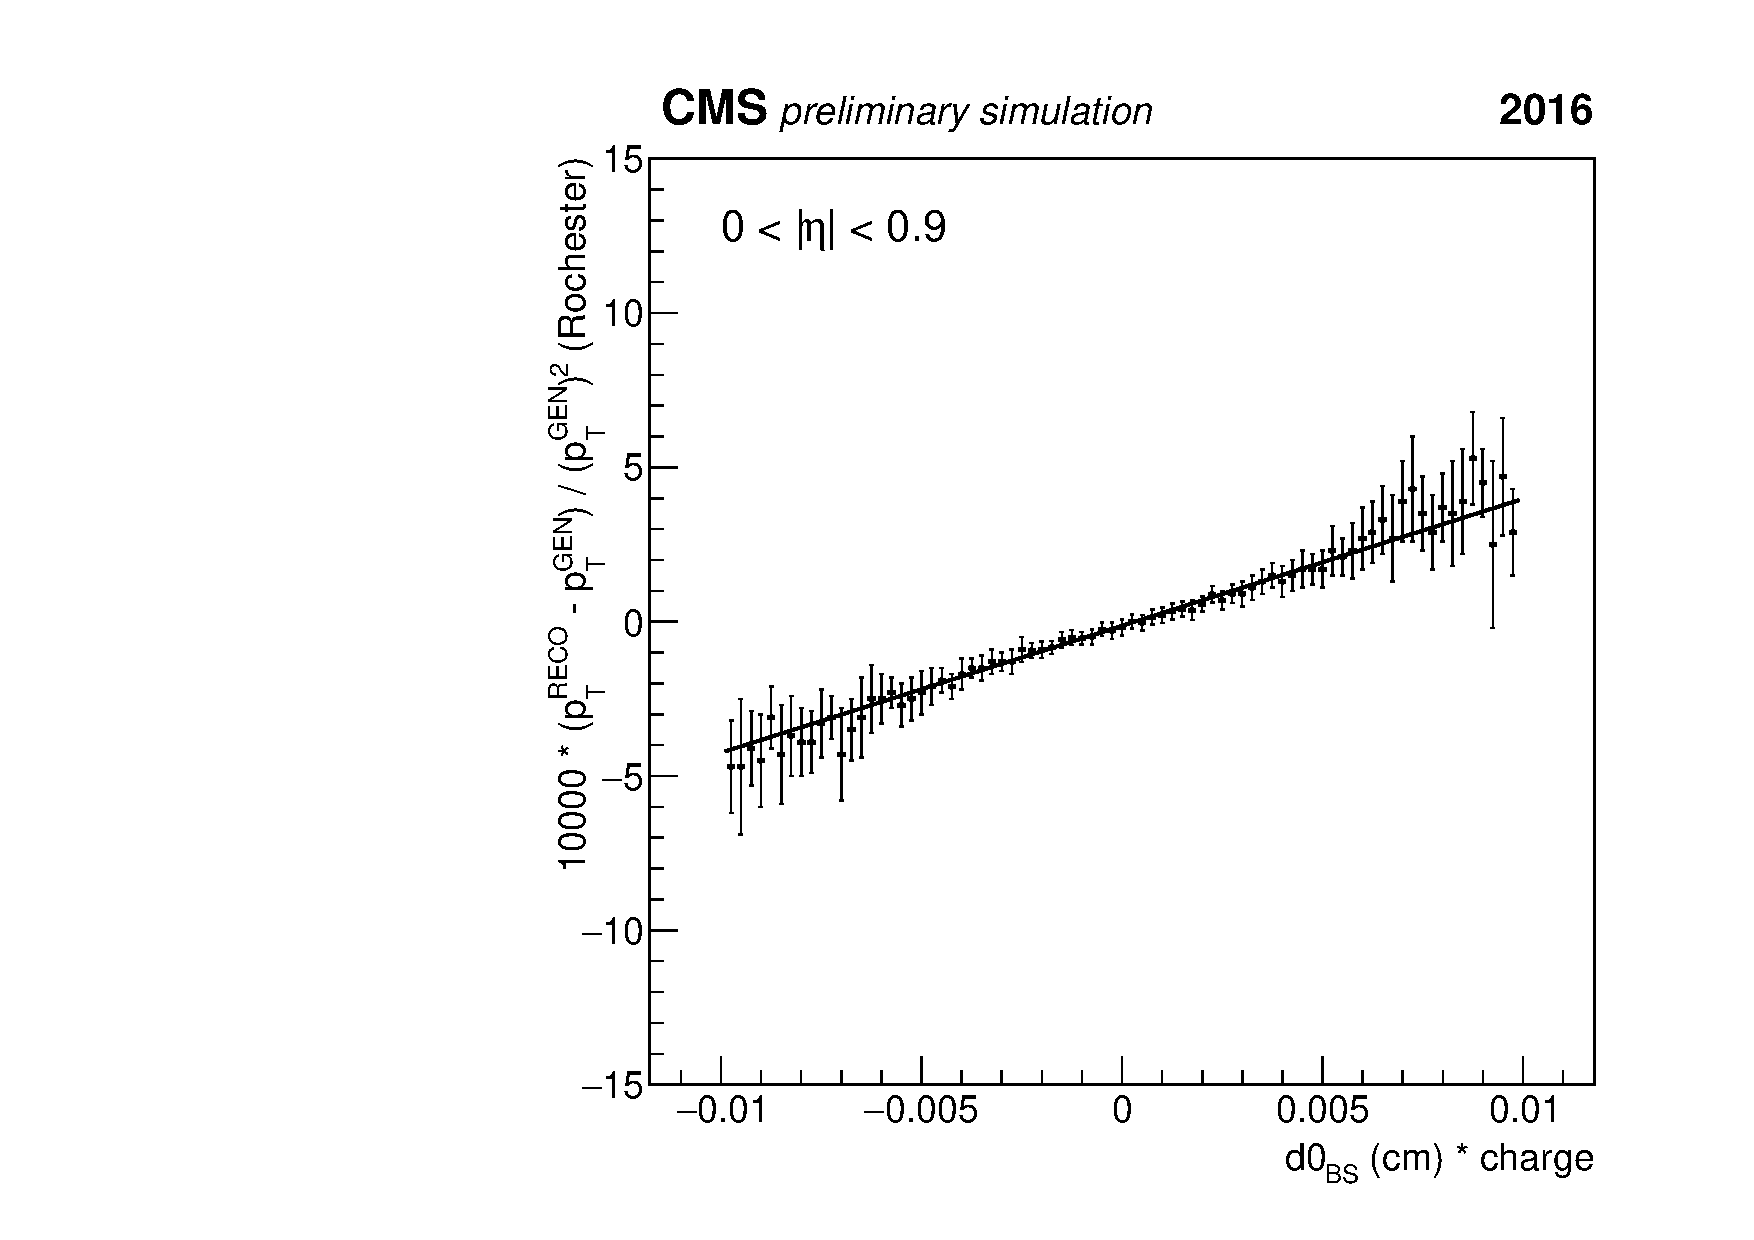
\includegraphics[width=0.45\textwidth]{pics/muon_corr/GeoFit/fit_results/d0_pt_BS_eg.pdf}
      \caption{Example plots showing the correlation between $(\pt^{reco}-\pt^{gen})/ (\pt^{gen})^{2}$ and $d_0 \times$ charge.
               The vertices used for the $d_0$ calculation are the PV (left) and the BS (right). 
               The PV plot shows a modulated dependence from expectation while the BS plot shows a linear shape as expected.
               Only barrel tracks from 2016 data are shown as examples. 
               Plots of other |\eta| regions and other data-taking periods show a similar behavior.
               Plots credit to Efe Yigitbasi.}
      \label{fig:pv_vs_bs_fits}
\end{figure*}

The $(\pt^{reco}-\pt^{gen})/ (\pt^{gen})^{2}$ vs $d_0$ correlation is found to be different in different |\eta| regions and data-taking periods: 
different |\eta| regions are covered by different detector components, and there have been upgrades on the detector and the reconstruction algorithm between different data-taking periods.
Overall, the $(\pt^{reco}-\pt^{gen})/ (\pt^{gen})^{2}$ vs $d_0$ correlation is evaluated by three years (2016, 2017, 2018) and 
three |\eta| regions (barrel, overlap, endcap), shown in Figure~\ref{fig:geofit_param_2016} for 2016, ~\ref{fig:geofit_param_2017} for 2017, and ~\ref{fig:geofit_param_2018} for 2018.
Each of the plots is fit with a linear function, whose best fit parameters are also shown in the plot.

\begin{figure*}[!htb]
      \centering
      \captionsetup{justification=justified}
      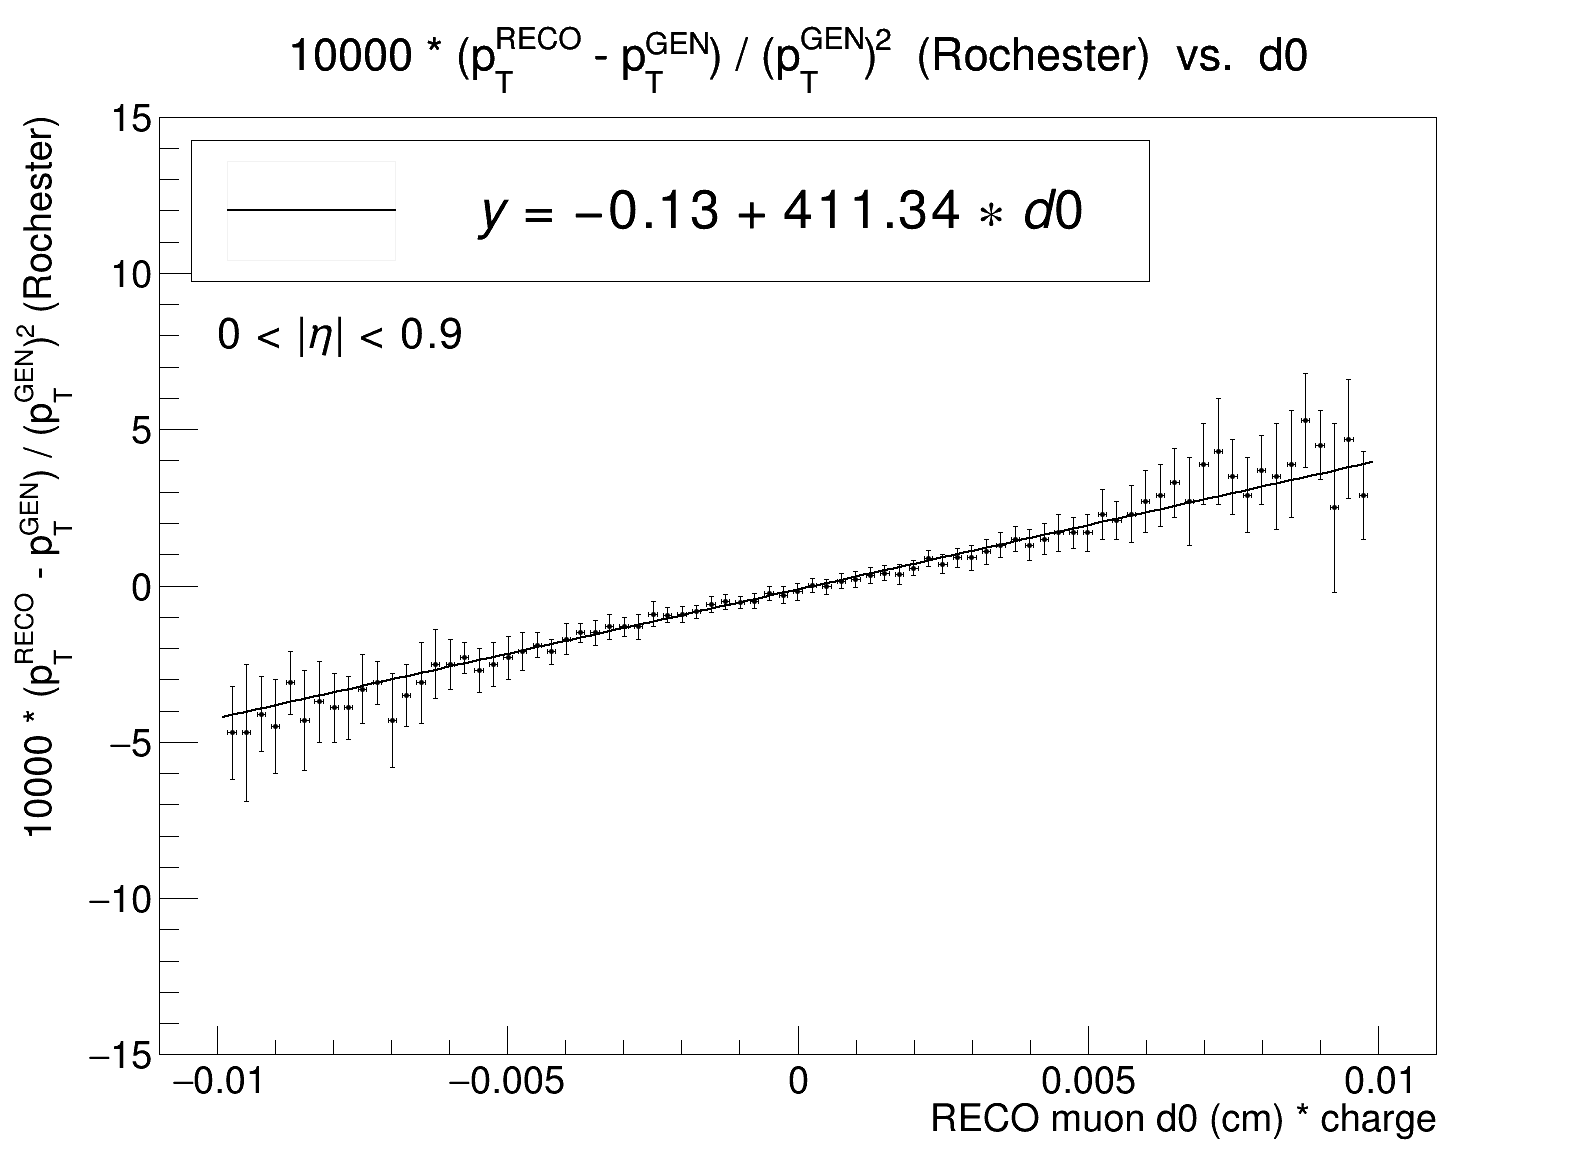
\includegraphics[width=0.32\textwidth]{pics/muon_corr/GeoFit/fit_results/2016_DY_eta_0_0p9_dRelPt2p0_Roch.png}
      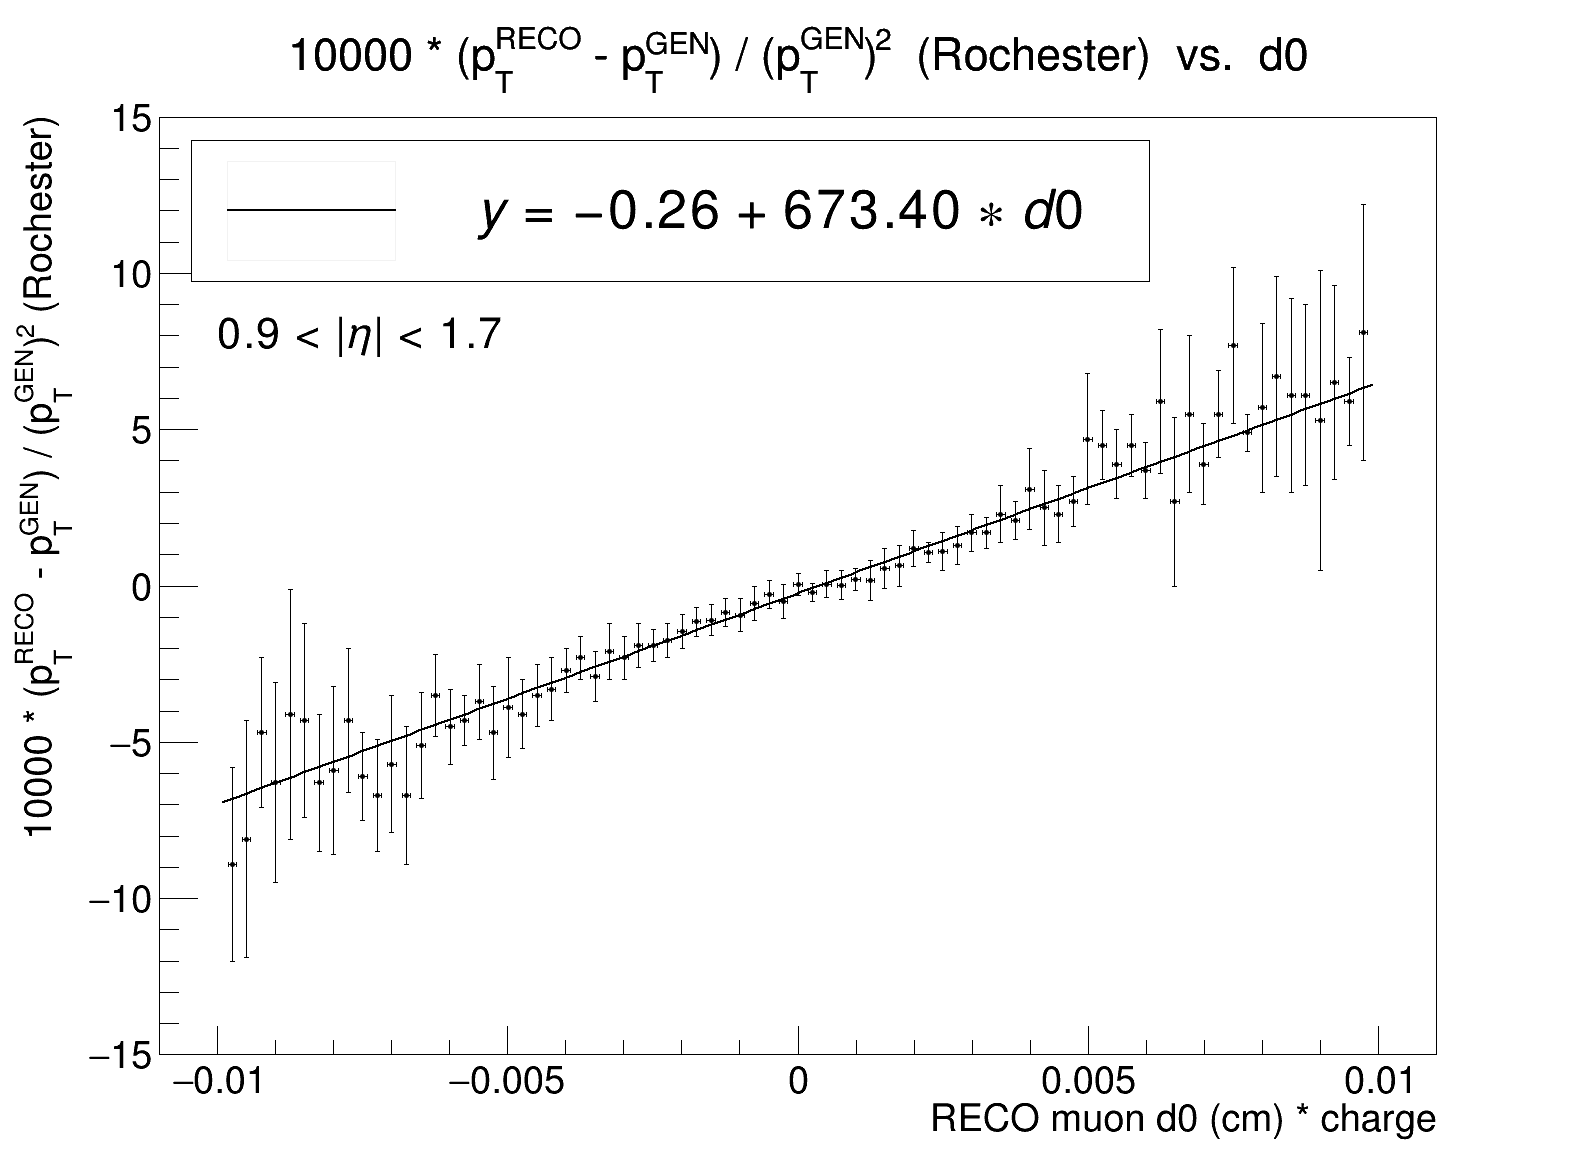
\includegraphics[width=0.32\textwidth]{pics/muon_corr/GeoFit/fit_results/2016_DY_eta_0p9_1p7_dRelPt2p0_Roch.png}
      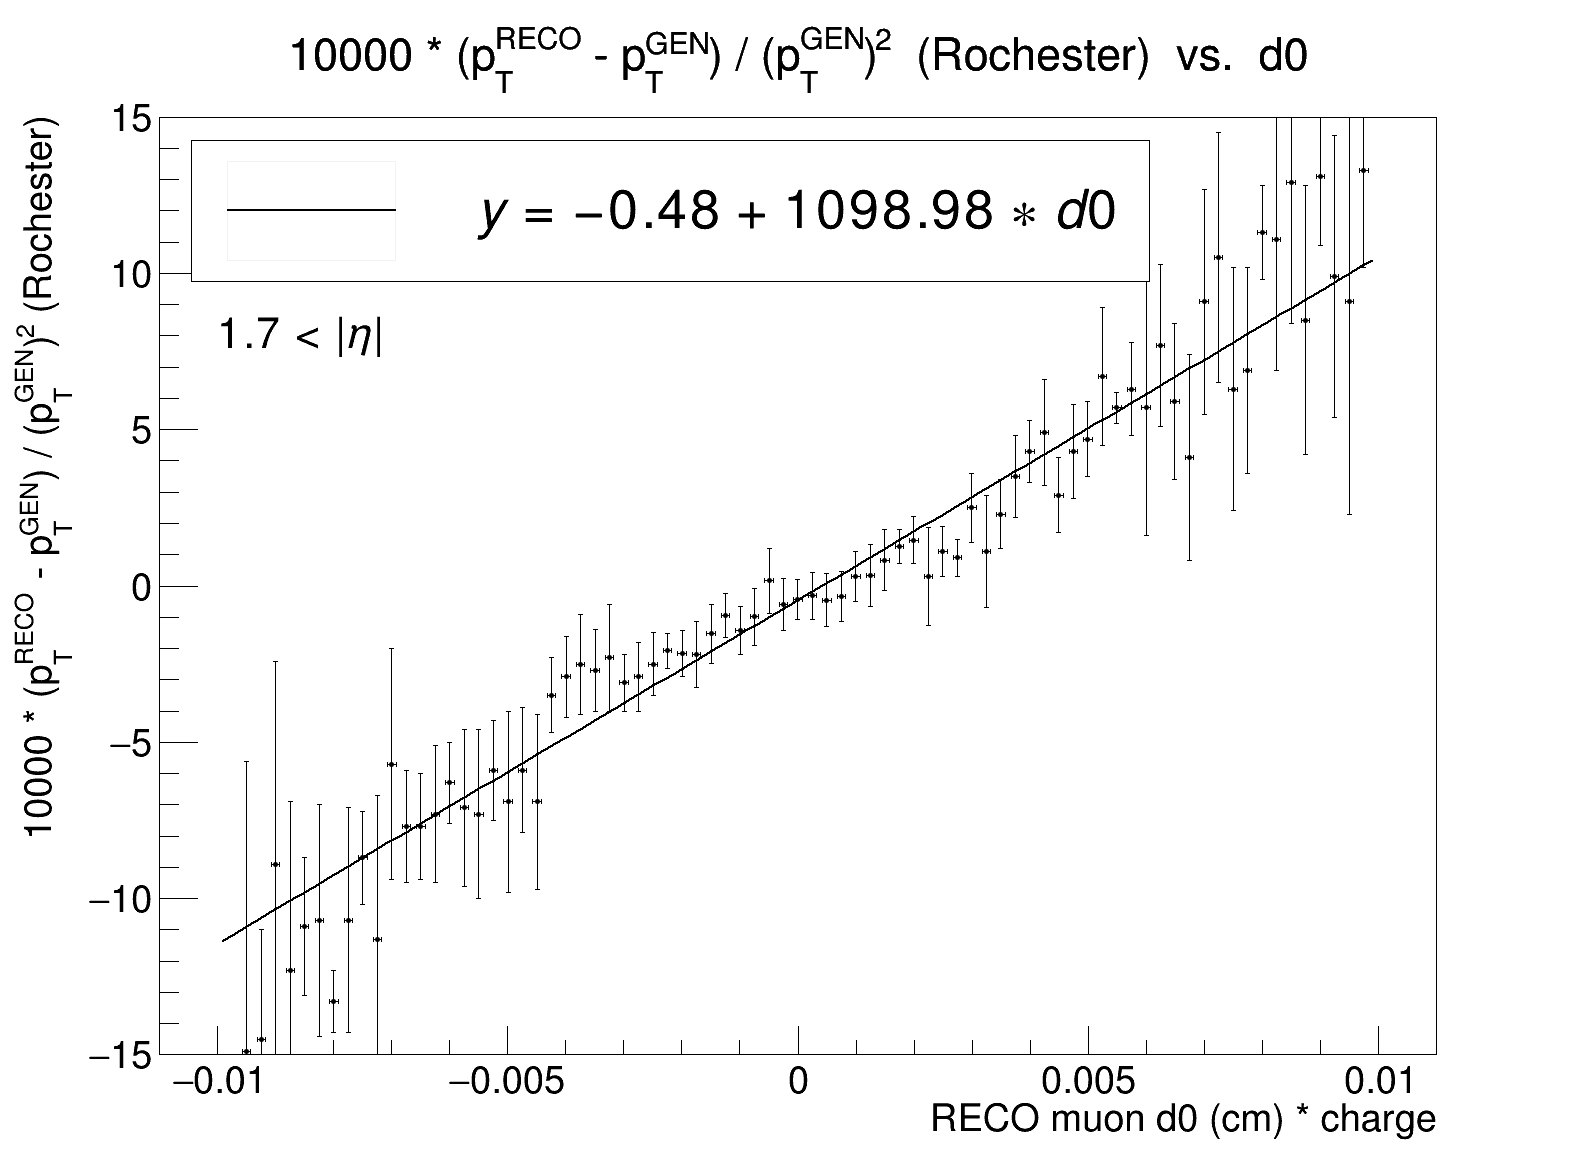
\includegraphics[width=0.32\textwidth]{pics/muon_corr/GeoFit/fit_results/2016_DY_eta_1p7_inf_dRelPt2p0_Roch.png}
      \caption{Plots for the $(\pt^{reco}-\pt^{gen})/ (\pt^{gen})^{2}$ vs $d_0$ correlation in the 2016 \DY simulation, 
               and the linear fits to them. Muon tracks are divided into three different |\eta| regions:
               $|\eta| <$ 0.9 (left), 0.9 $< |\eta| <$ 1.7 (middle), and 1.7 $< |\eta|$ (right).
               Plots credit to Efe Yigitbasi.}
      \label{fig:geofit_param_2016}
\end{figure*}

\begin{figure*}[!htb]
      \centering
      \captionsetup{justification=justified}
      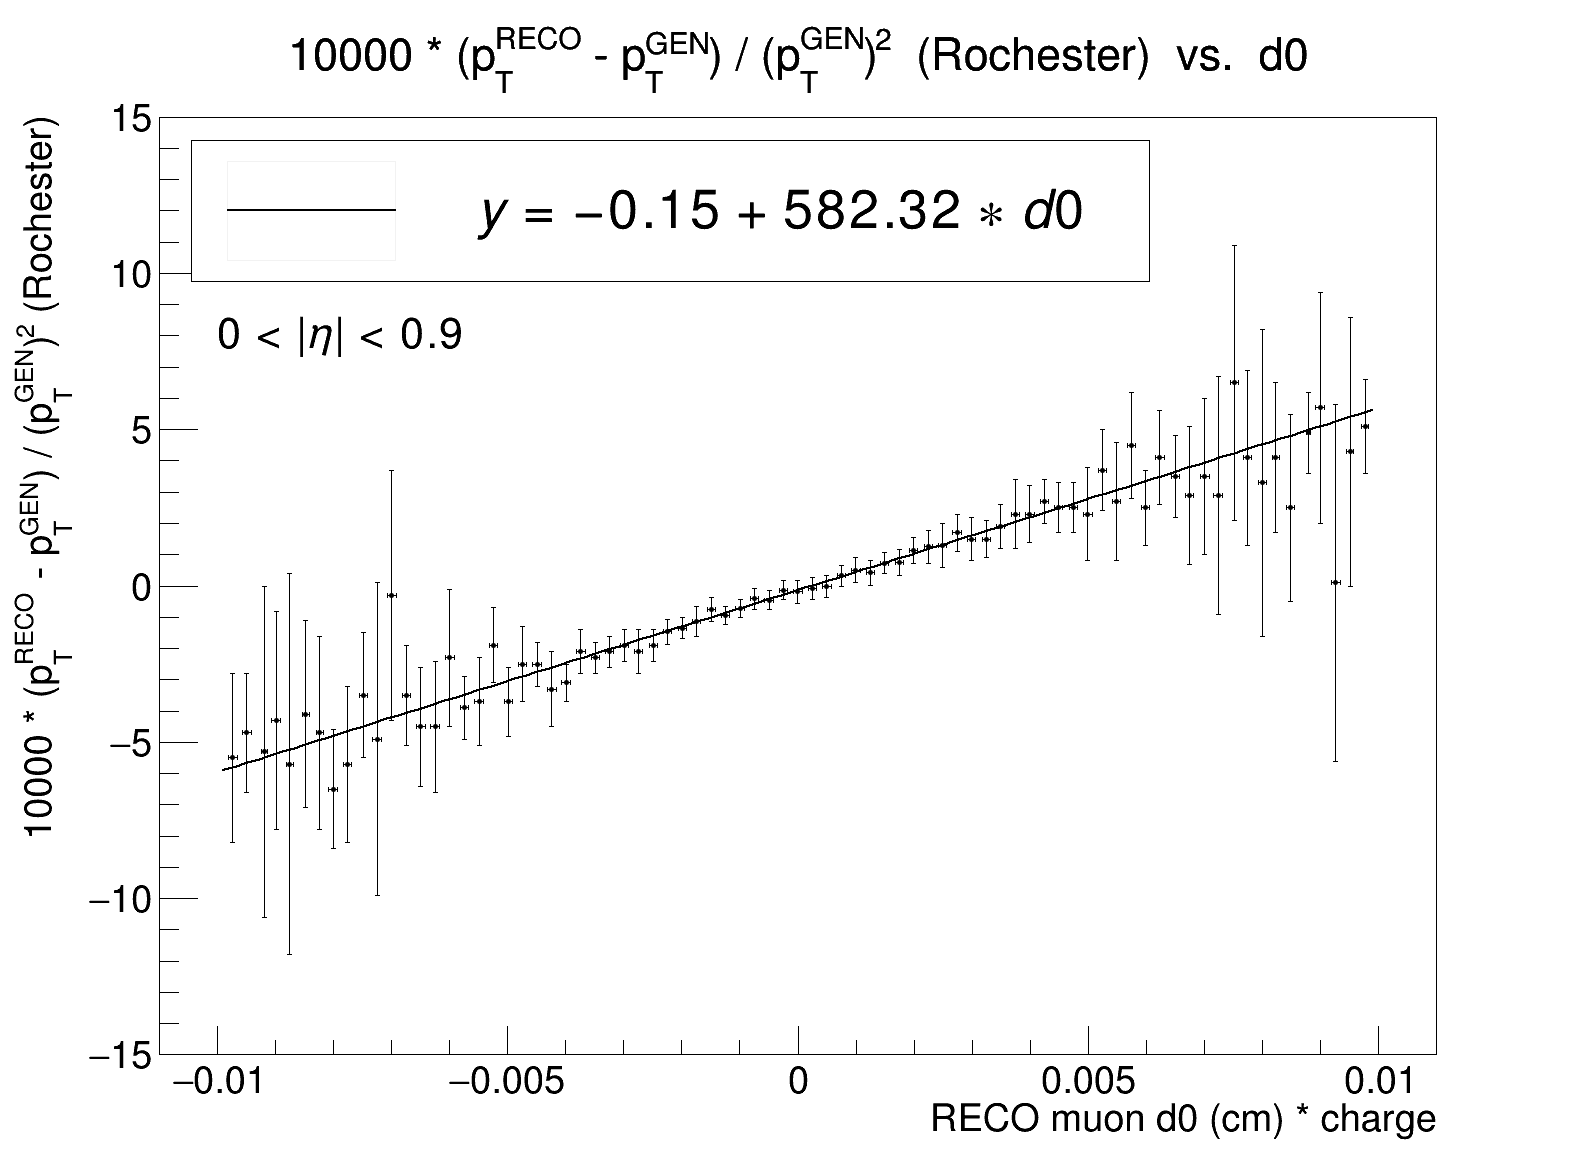
\includegraphics[width=0.32\textwidth]{pics/muon_corr/GeoFit/fit_results/2017_DY_eta_0_0p9_dRelPt2p0_Roch.png}
      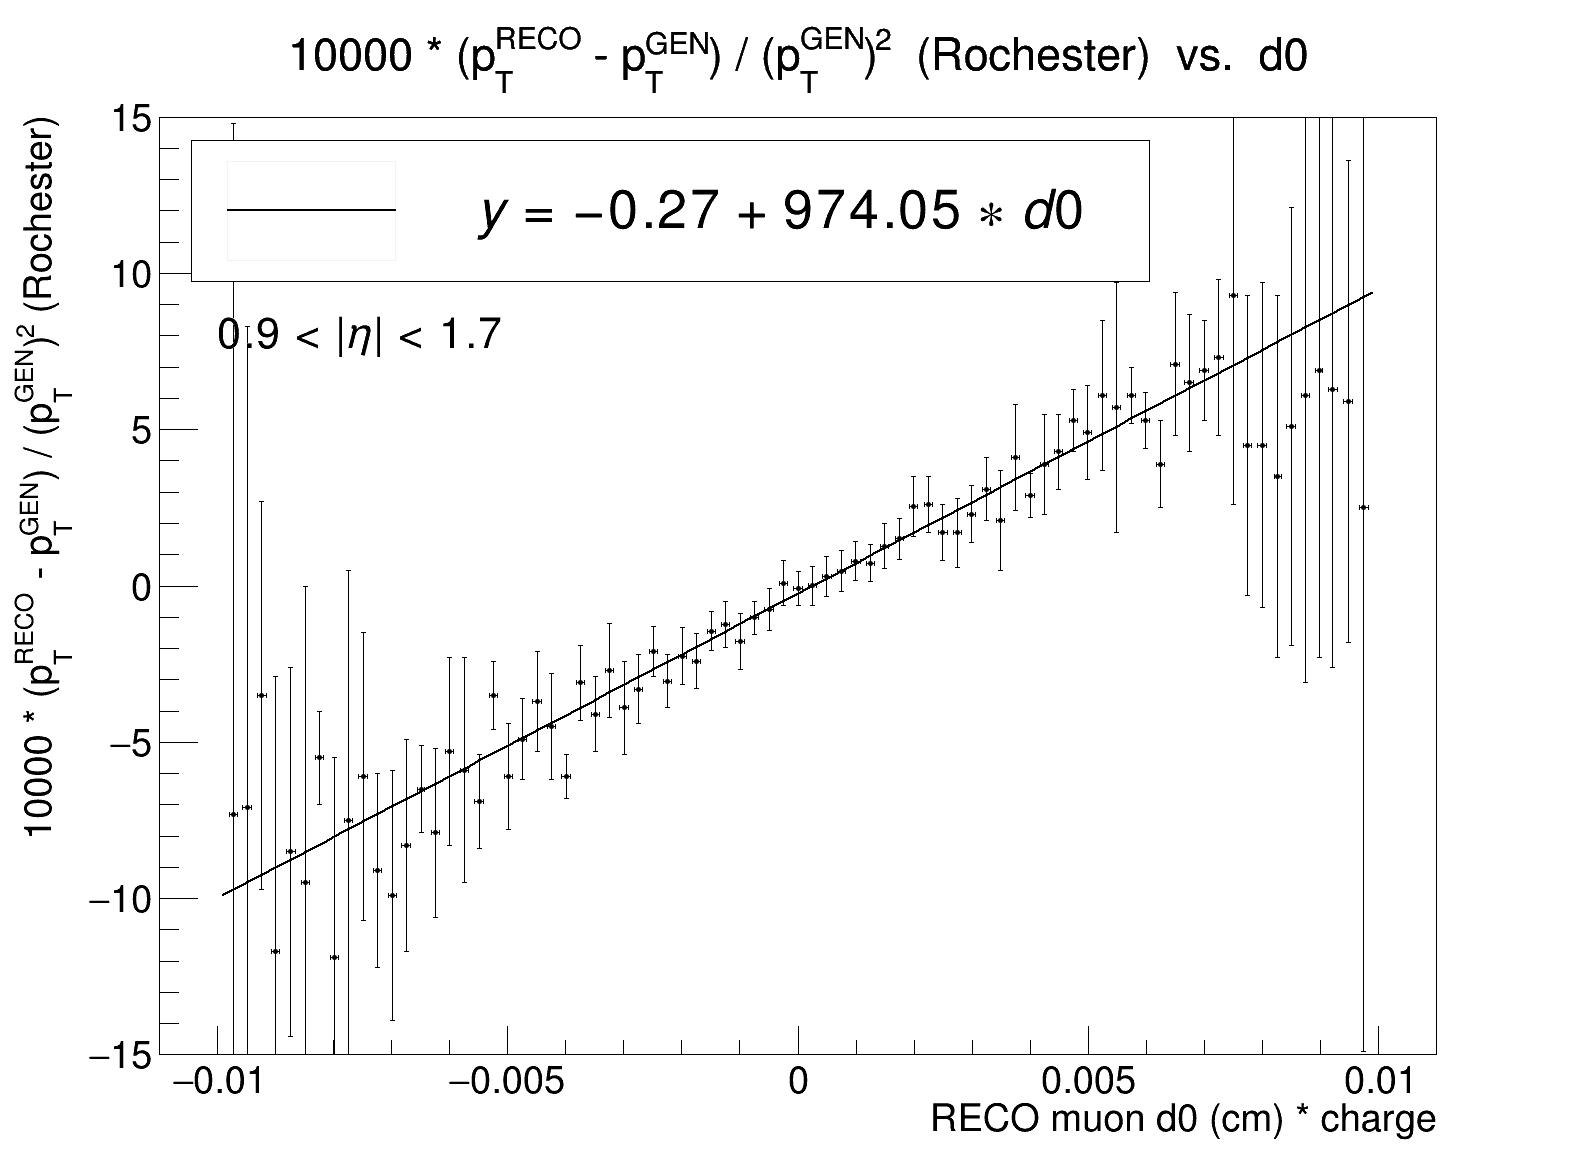
\includegraphics[width=0.32\textwidth]{pics/muon_corr/GeoFit/fit_results/2017_DY_eta_0p9_1p7_dRelPt2p0_Roch.png}
      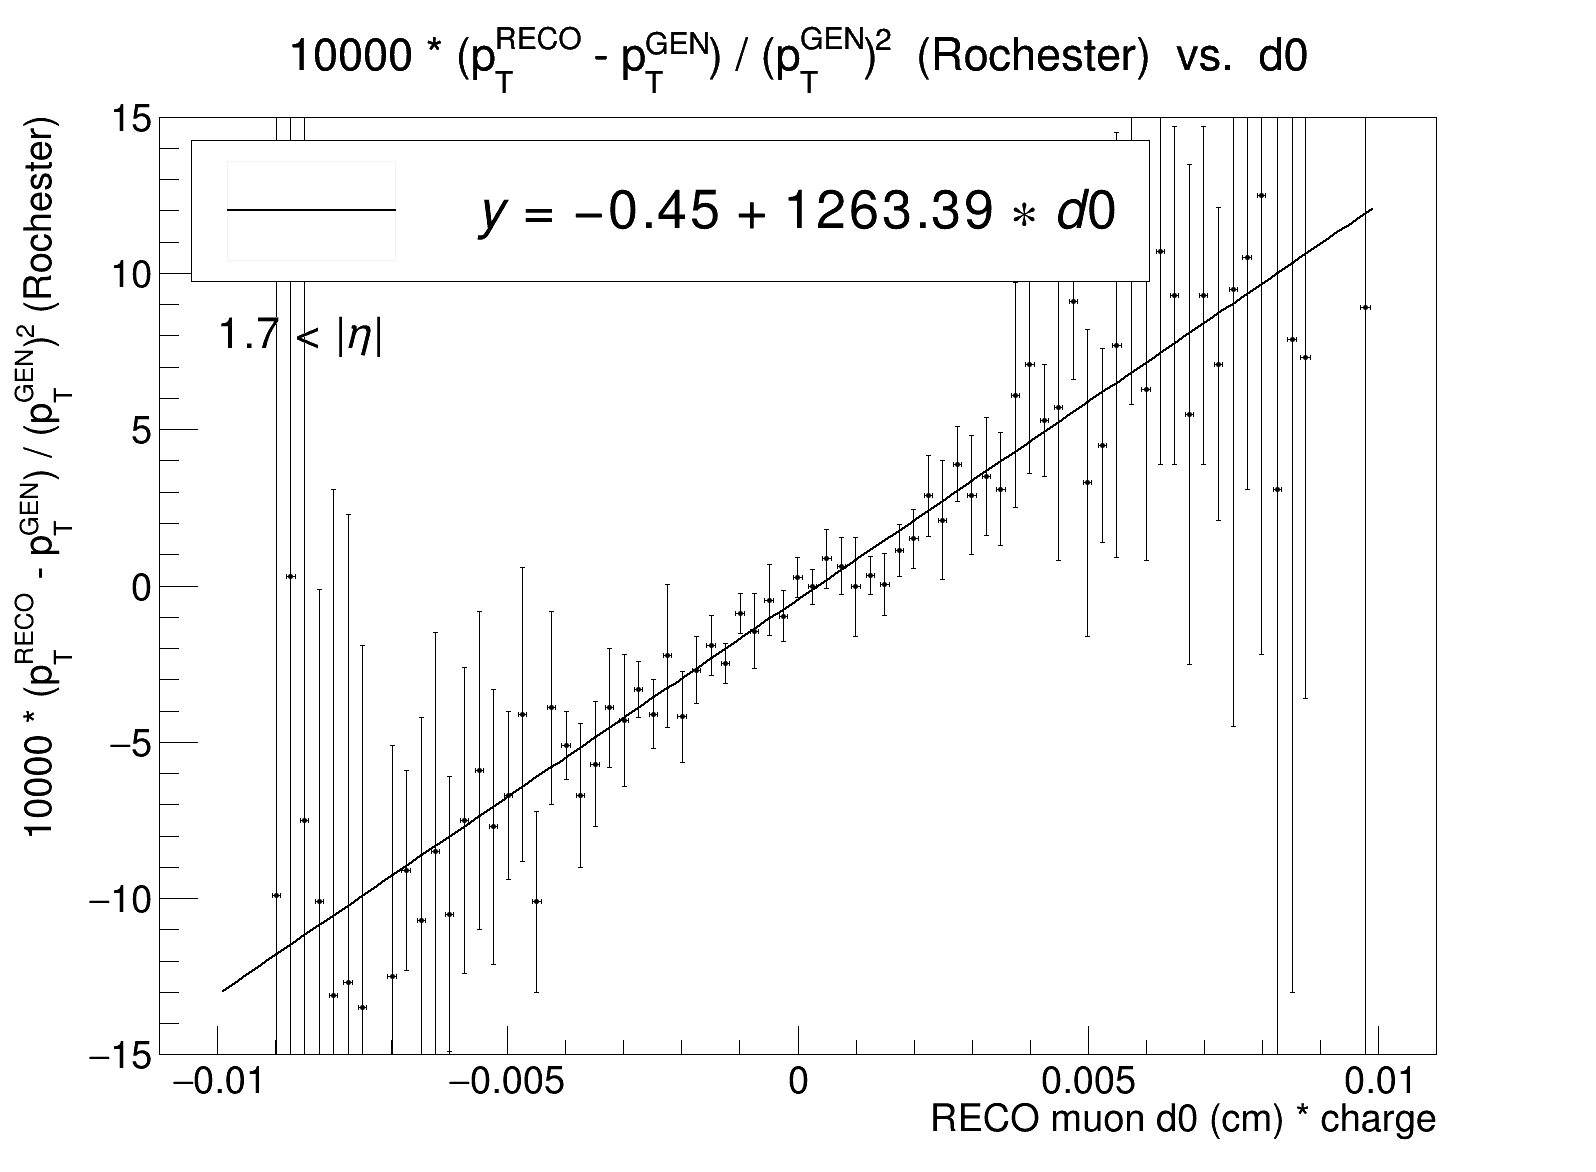
\includegraphics[width=0.32\textwidth]{pics/muon_corr/GeoFit/fit_results/2017_DY_eta_1p7_inf_dRelPt2p0_Roch.png}
      \caption{Plots for the $(\pt^{reco}-\pt^{gen})/ (\pt^{gen})^{2}$ vs $d_0$ correlation in the 2017 \DY simulation, 
               and the linear fits to them. Muon tracks are divided into three different |\eta| regions:
               $|\eta| <$ 0.9 (left), 0.9 $< |\eta| <$ 1.7 (middle), and 1.7 $< |\eta|$ (right).
               Plots credit to Efe Yigitbasi.}
      \label{fig:geofit_param_2017}
\end{figure*}

\begin{figure*}[!htb]
      \centering
      \captionsetup{justification=justified}
      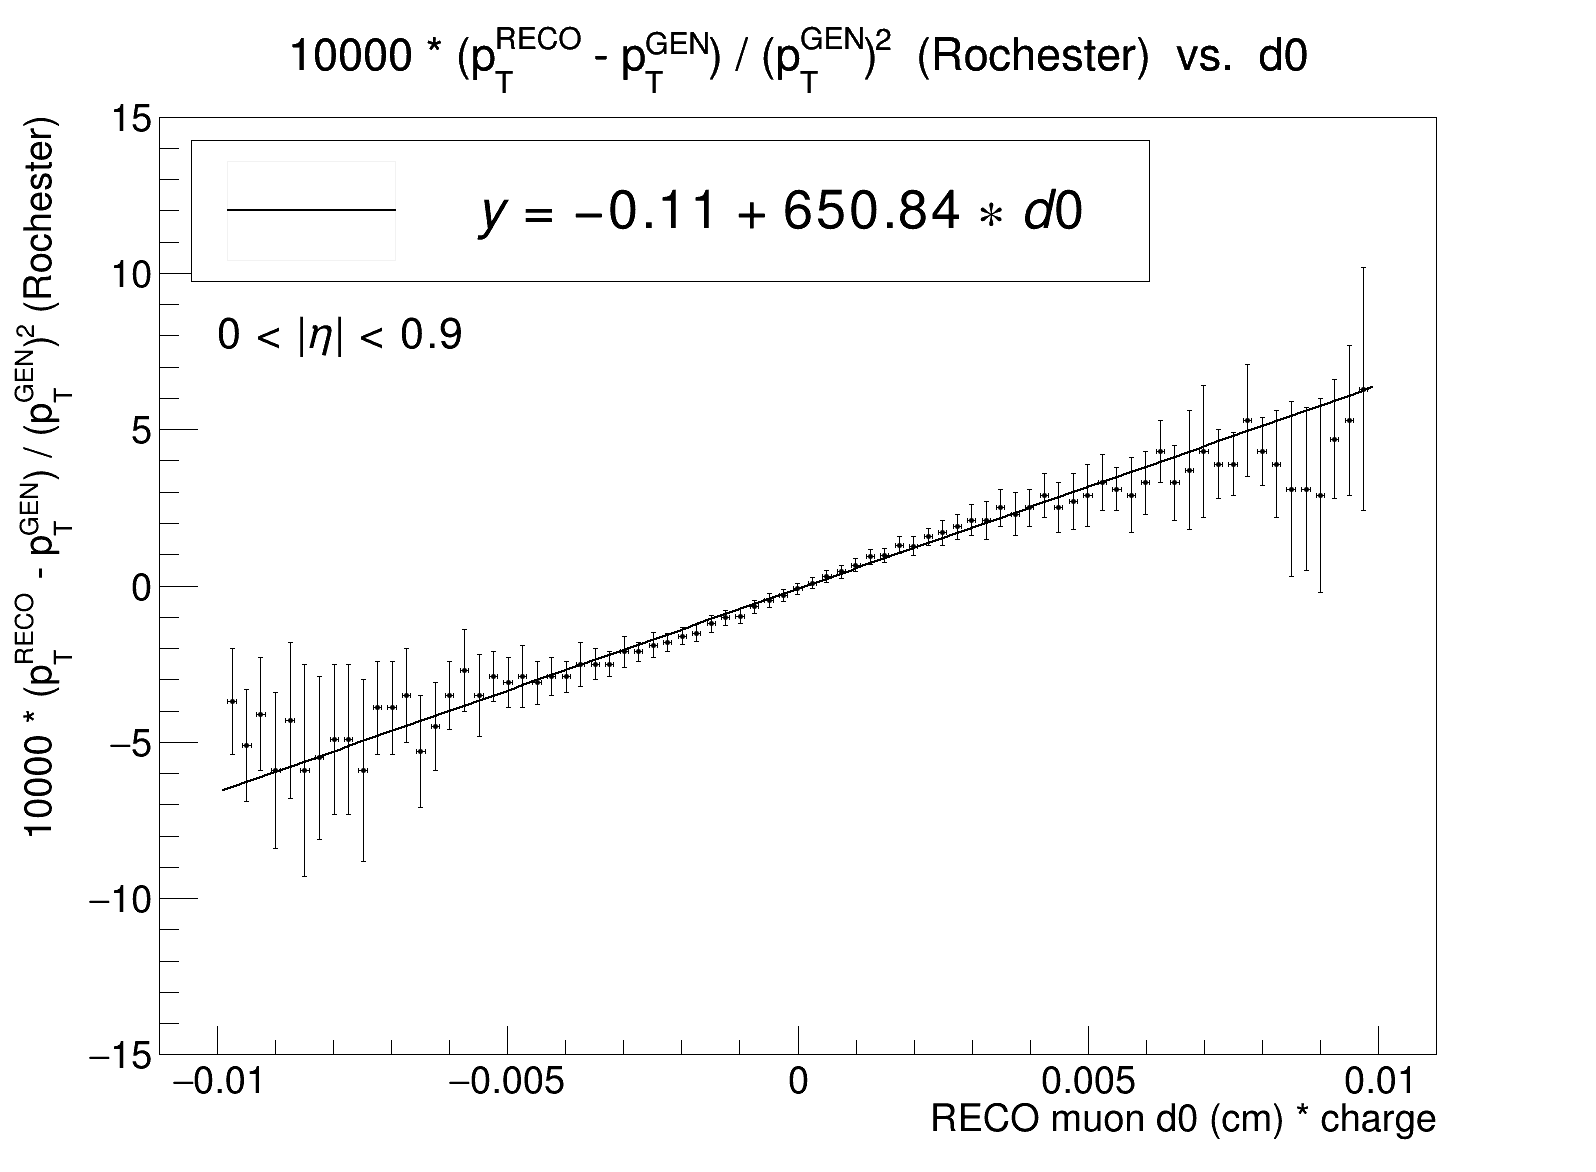
\includegraphics[width=0.32\textwidth]{pics/muon_corr/GeoFit/fit_results/2018_DY_eta_0_0p9_dRelPt2p0_Roch.png}
      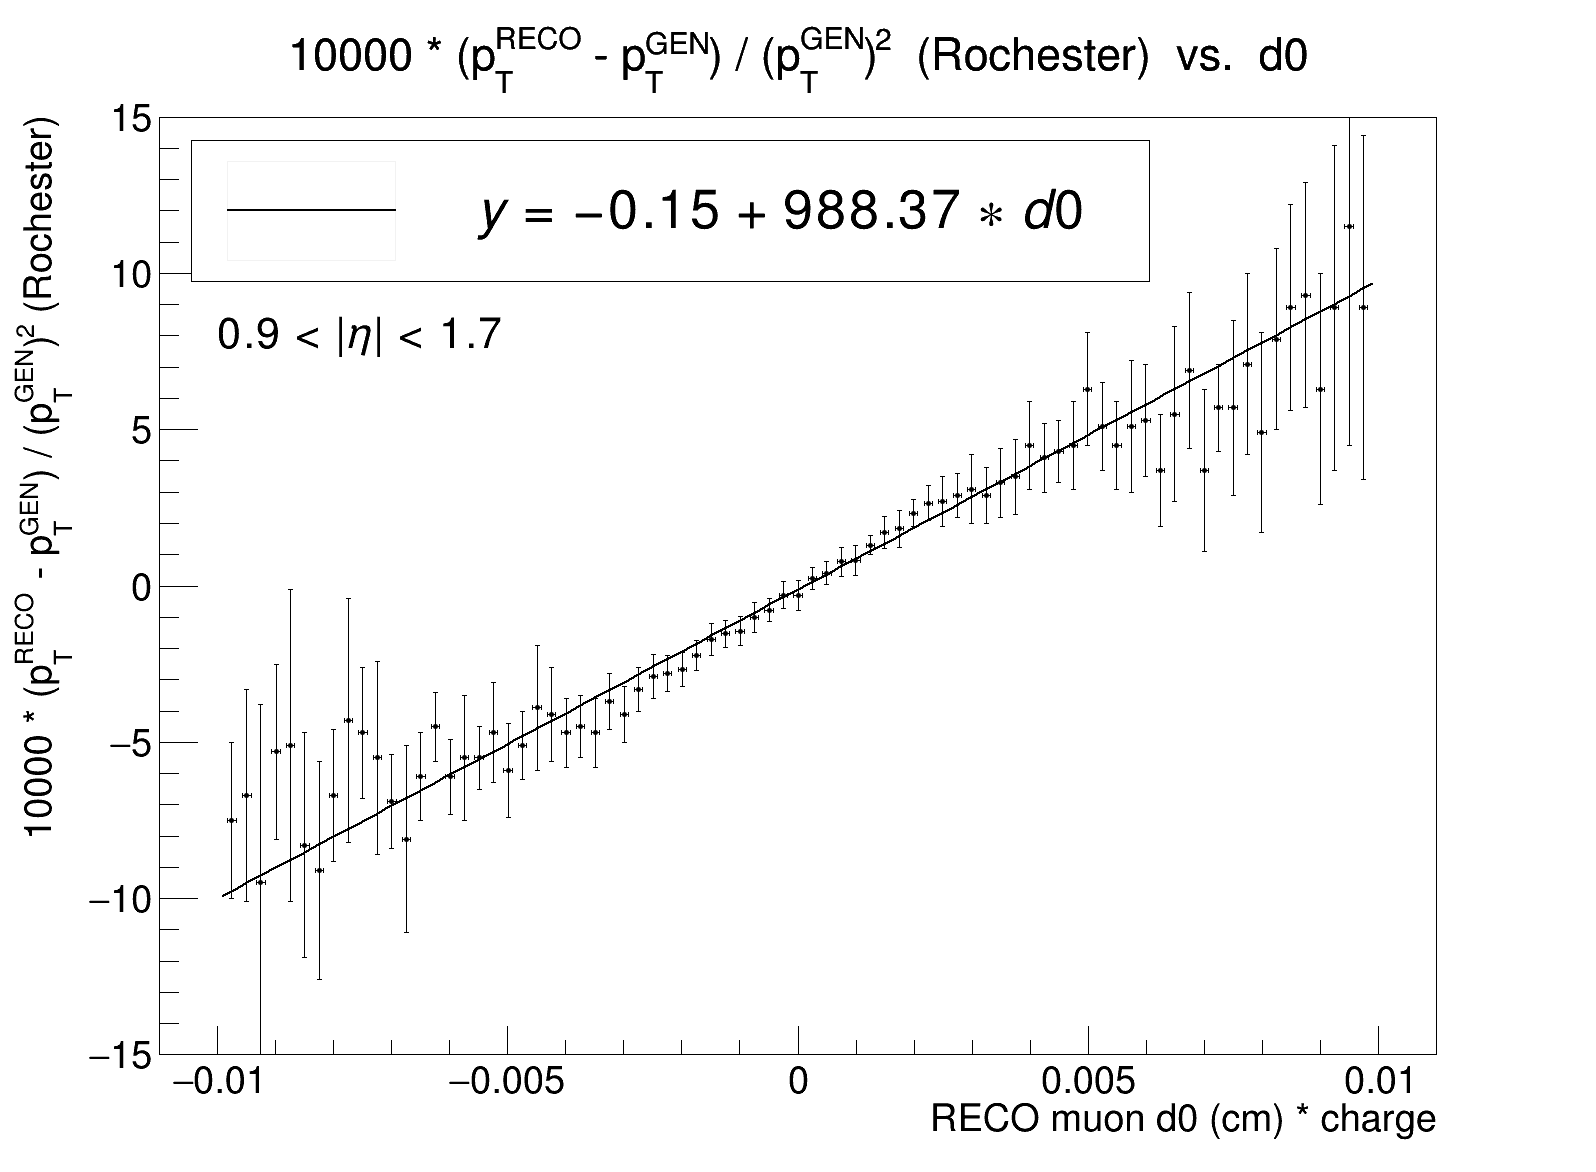
\includegraphics[width=0.32\textwidth]{pics/muon_corr/GeoFit/fit_results/2018_DY_eta_0p9_1p7_dRelPt2p0_Roch.png}
      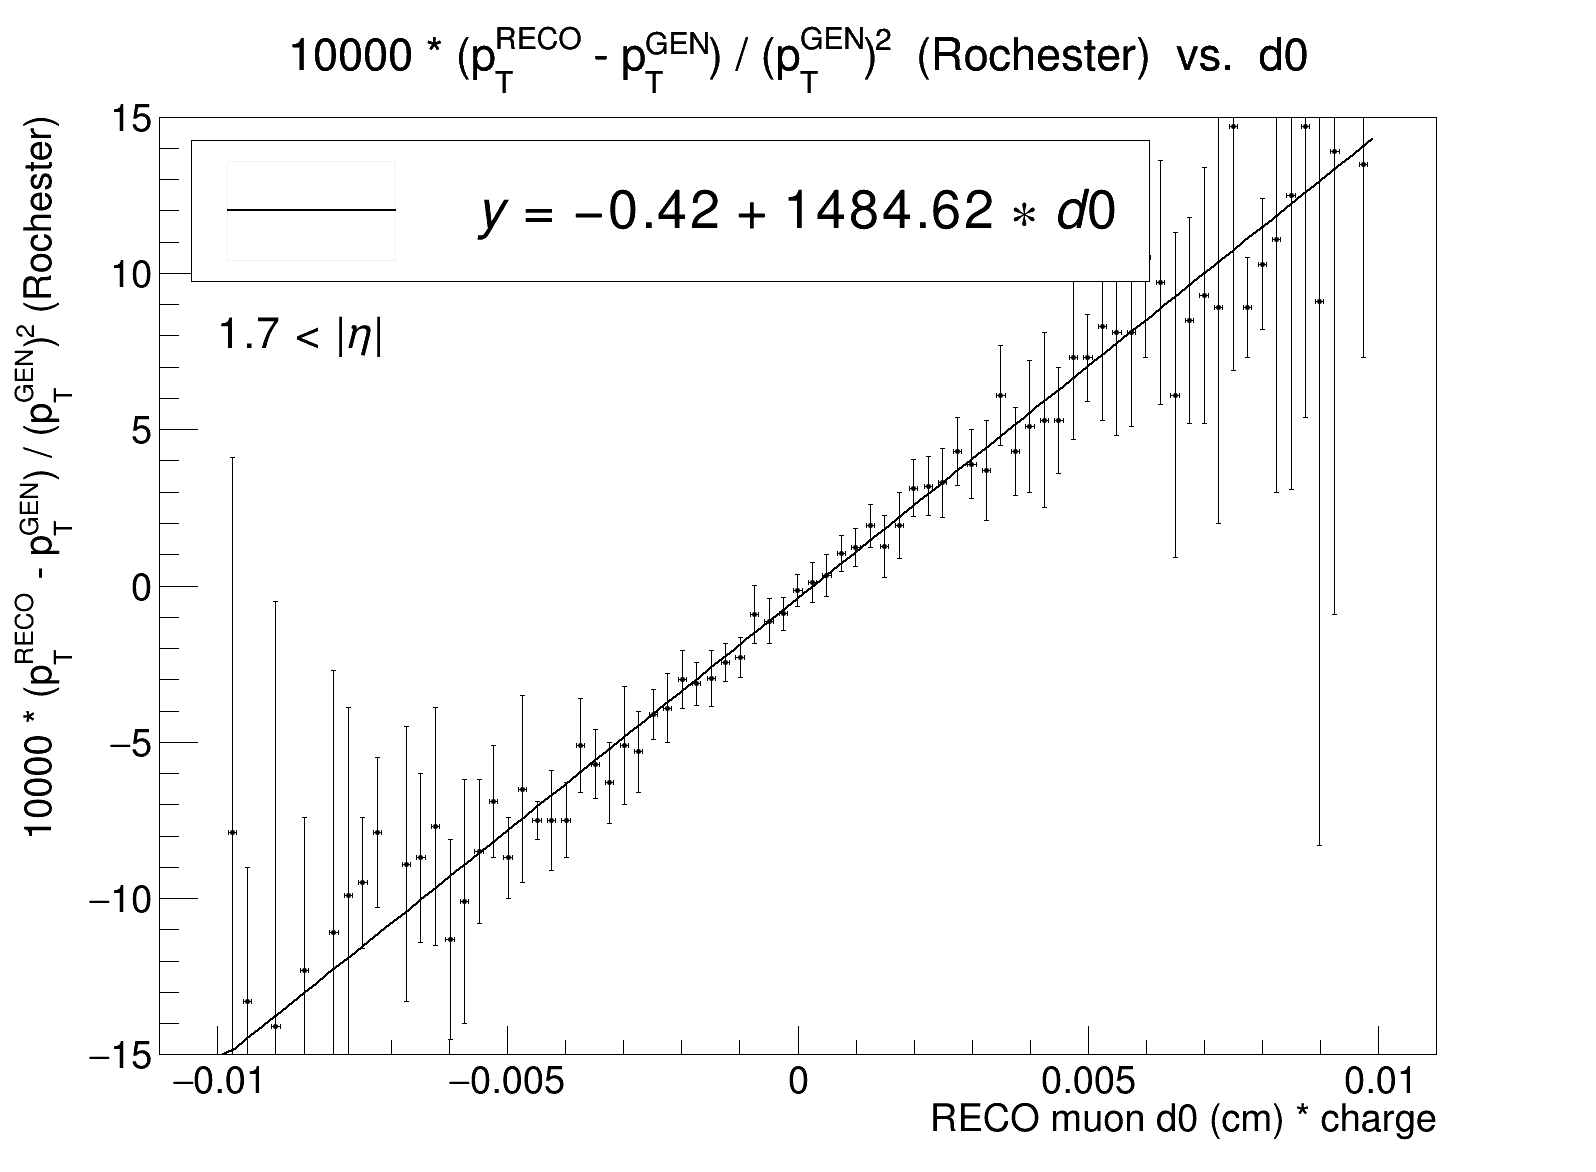
\includegraphics[width=0.32\textwidth]{pics/muon_corr/GeoFit/fit_results/2018_DY_eta_1p7_inf_dRelPt2p0_Roch.png}
      \caption{Plots for the $(\pt^{reco}-\pt^{gen})/ (\pt^{gen})^{2}$ vs $d_0$ correlation in the 2018 \DY simulation, 
               and the linear fits to them. Muon tracks are divided into three different |\eta| regions:
               $|\eta| <$ 0.9 (left), 0.9 $< |\eta| <$ 1.7 (middle), and 1.7 $< |\eta|$ (right).
               Plots credit to Efe Yigitbasi.}
      \label{fig:geofit_param_2018}
\end{figure*}

These fit results are applied as the analytic correction to muon \pt, 
based on the $d_0$, \pt, |\eta|, and charge of the muon.
The correction is applied to all muons in data and simulation in all categories in the \hmm analysis, 
unless the muon is tagged for \FSR.
The performance of this correction is detailed in Section~\ref{sec:perf_geofit}.

\subsection{Performance and validation}\label{sec:perf_geofit}

The \GeoFit removes the \pt dependence on $d_0$, 
whose overall effect on the \zmm peak is illustrated in Figure~\ref{fig:mucal_d0_run2}.
A clear trend in the \mmm is seen regarding $d_0$ before the \GeoFit, 
while no significant dependence remains after the correction.
As a side remark, the \mmm mismeasurement in Figure~\ref{fig:mucal_d0_run2} can be as large as 1.5 \GeV for extreme $d_0$ values,
but in data and simulation the distribution of the muon $d_0$ is roughly a Gaussian shape with a standard deviation around 15 \mum.
So most of the events are near the center of the plots, and the size of the correction is not as exaggerated as the values at the tails. 

\begin{figure*}[!htb]
      \centering
      \captionsetup{justification=justified}
      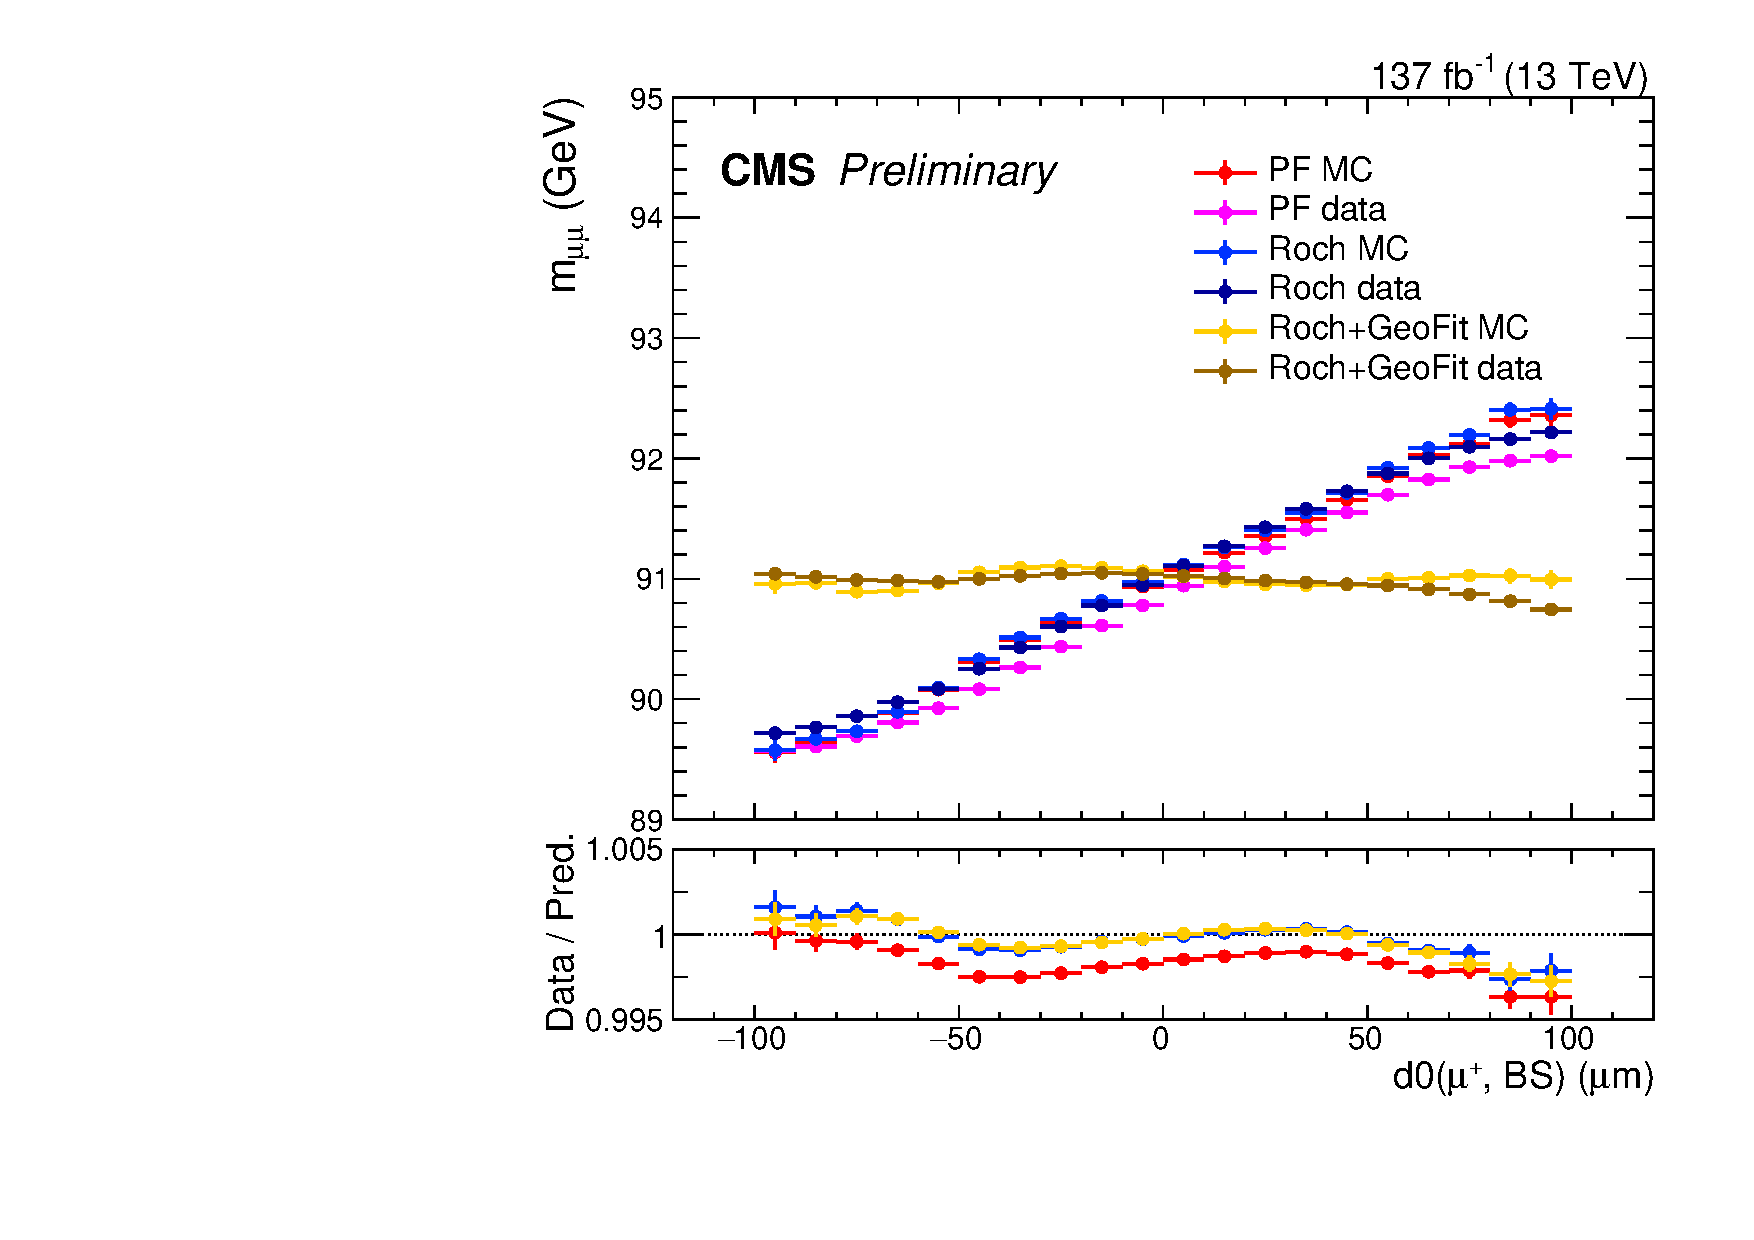
\includegraphics[width=0.45\textwidth]{pics/muon_corr/GeoFit/performance/muP_d0_summary_mean.pdf}
      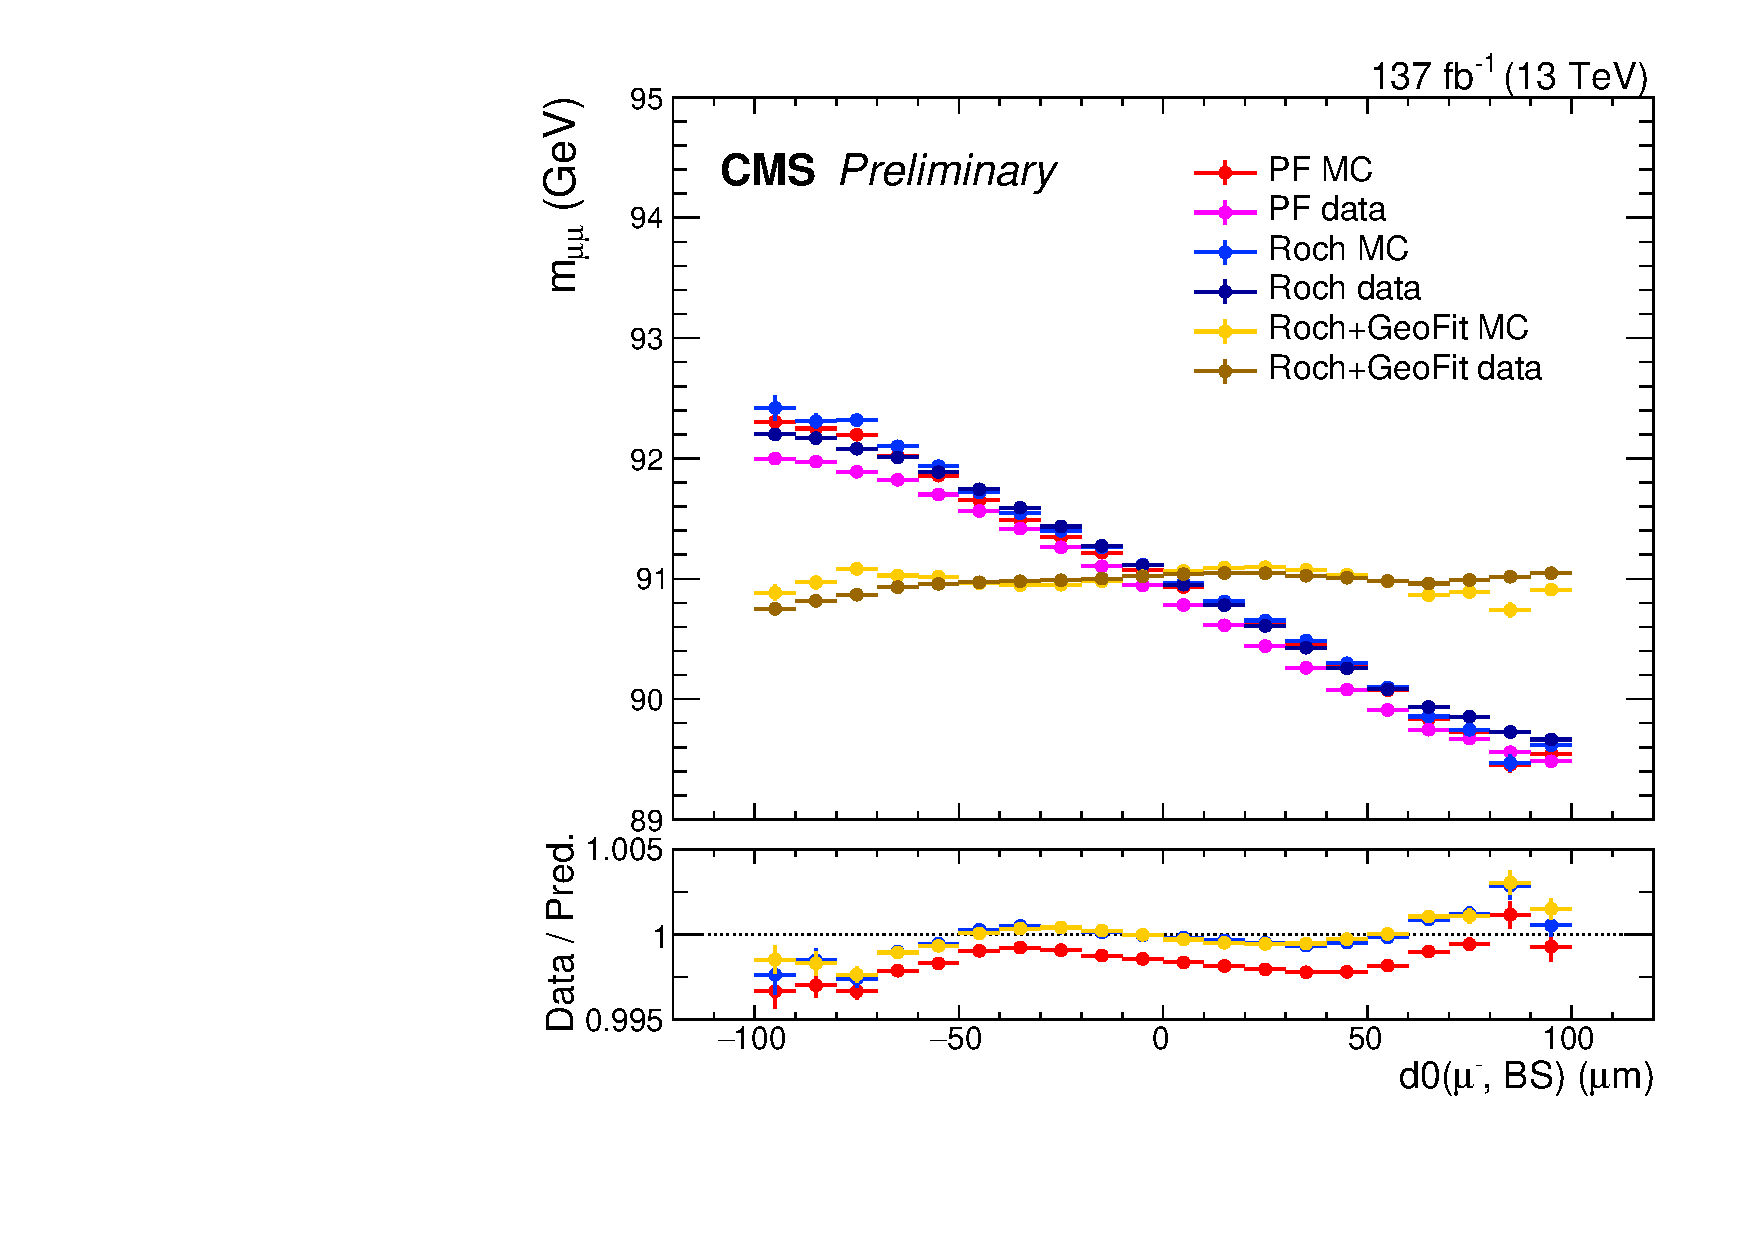
\includegraphics[width=0.45\textwidth]{pics/muon_corr/GeoFit/performance/muN_d0_summary_mean.pdf}
      \caption{Plots showing the \pt dependence on the $d_0$ value with different stages of muon correction.
               The plots compare the \zmm peak in data and simulation for three years (2016-2018) combined.
               All positively charged muons are put in the left plot and all negatively charged ones are put in the right plot.
               The $\pt-d_0$ dependence is reversed for positive and negative muons.
               }
      \label{fig:mucal_d0_run2}
\end{figure*}


\begin{figure*}[!htb]
      \centering
      \captionsetup{justification=justified}
      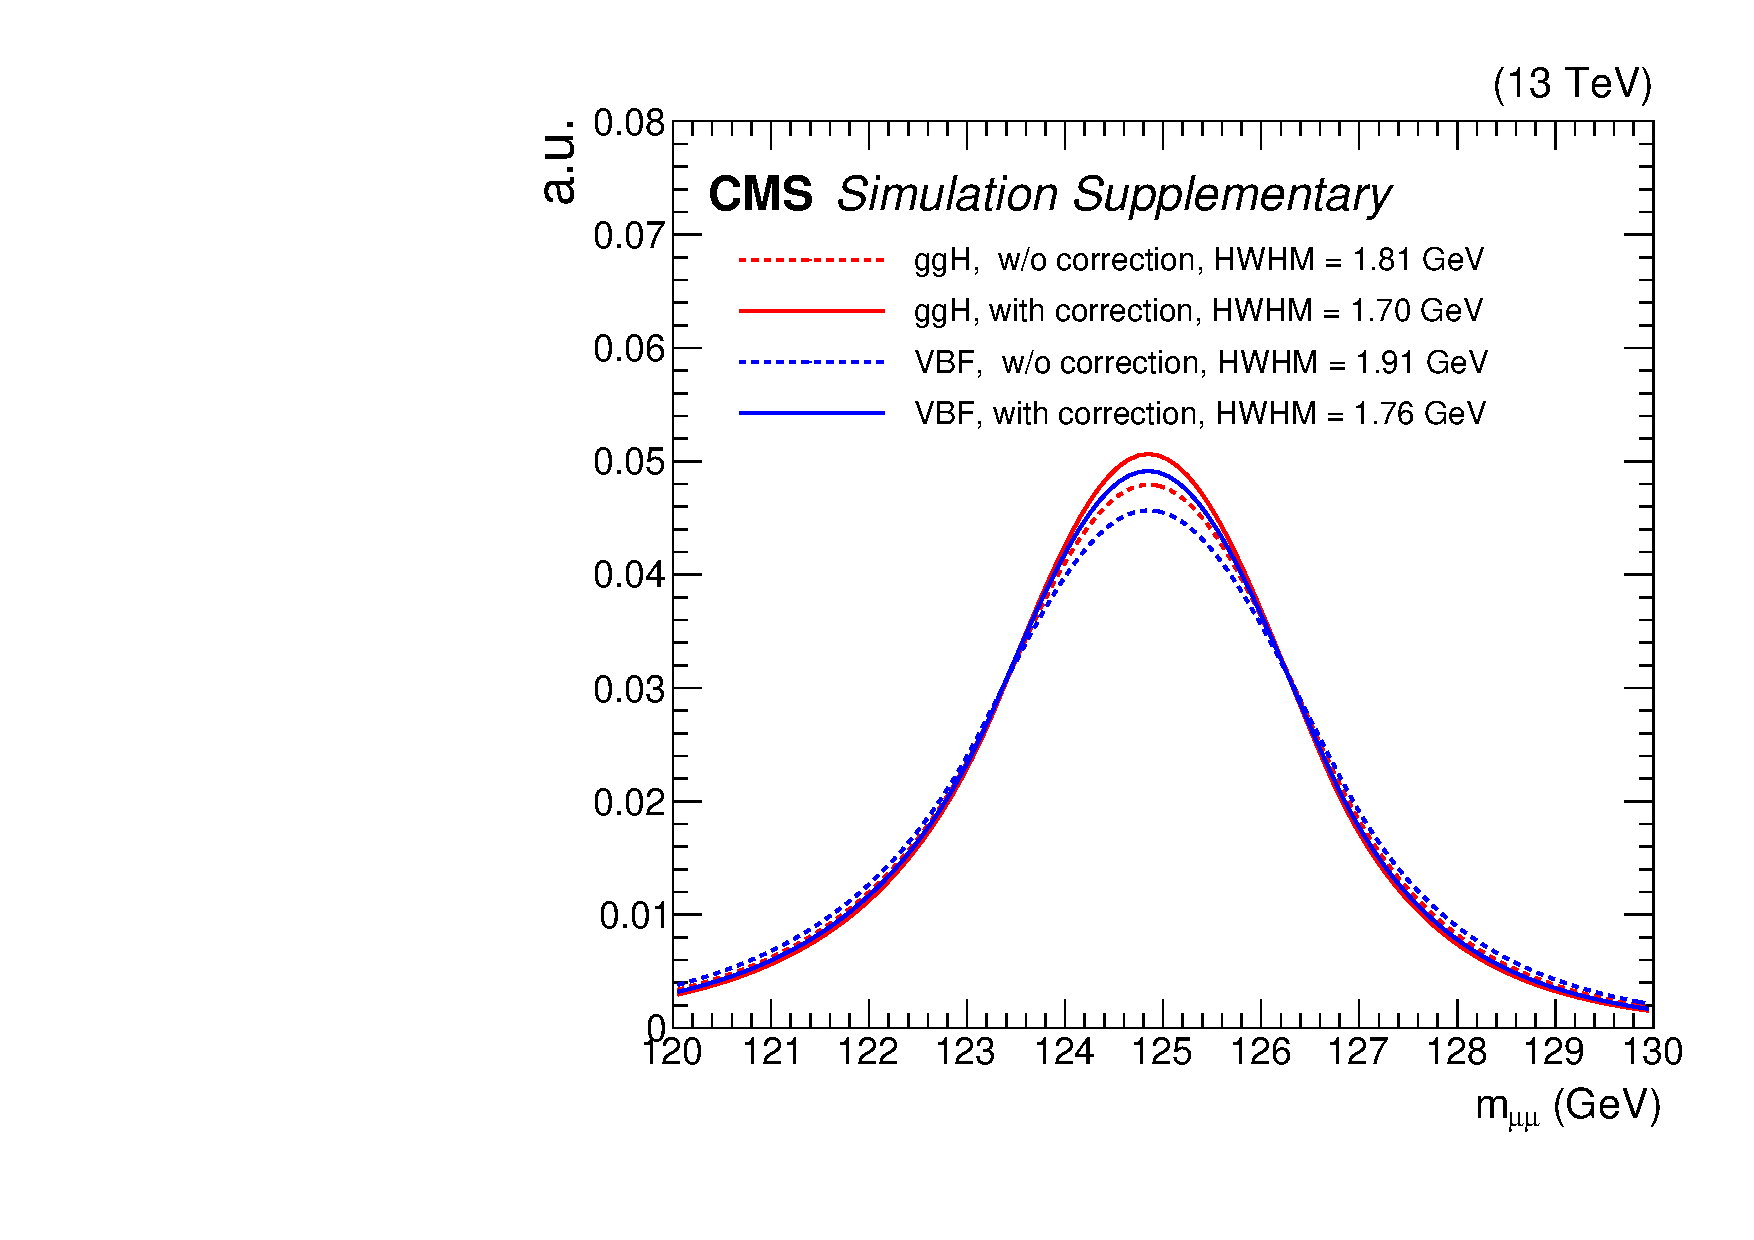
\includegraphics[width=0.45\textwidth]{pics/muon_corr/GeoFit/performance/ggHVBF.pdf}
      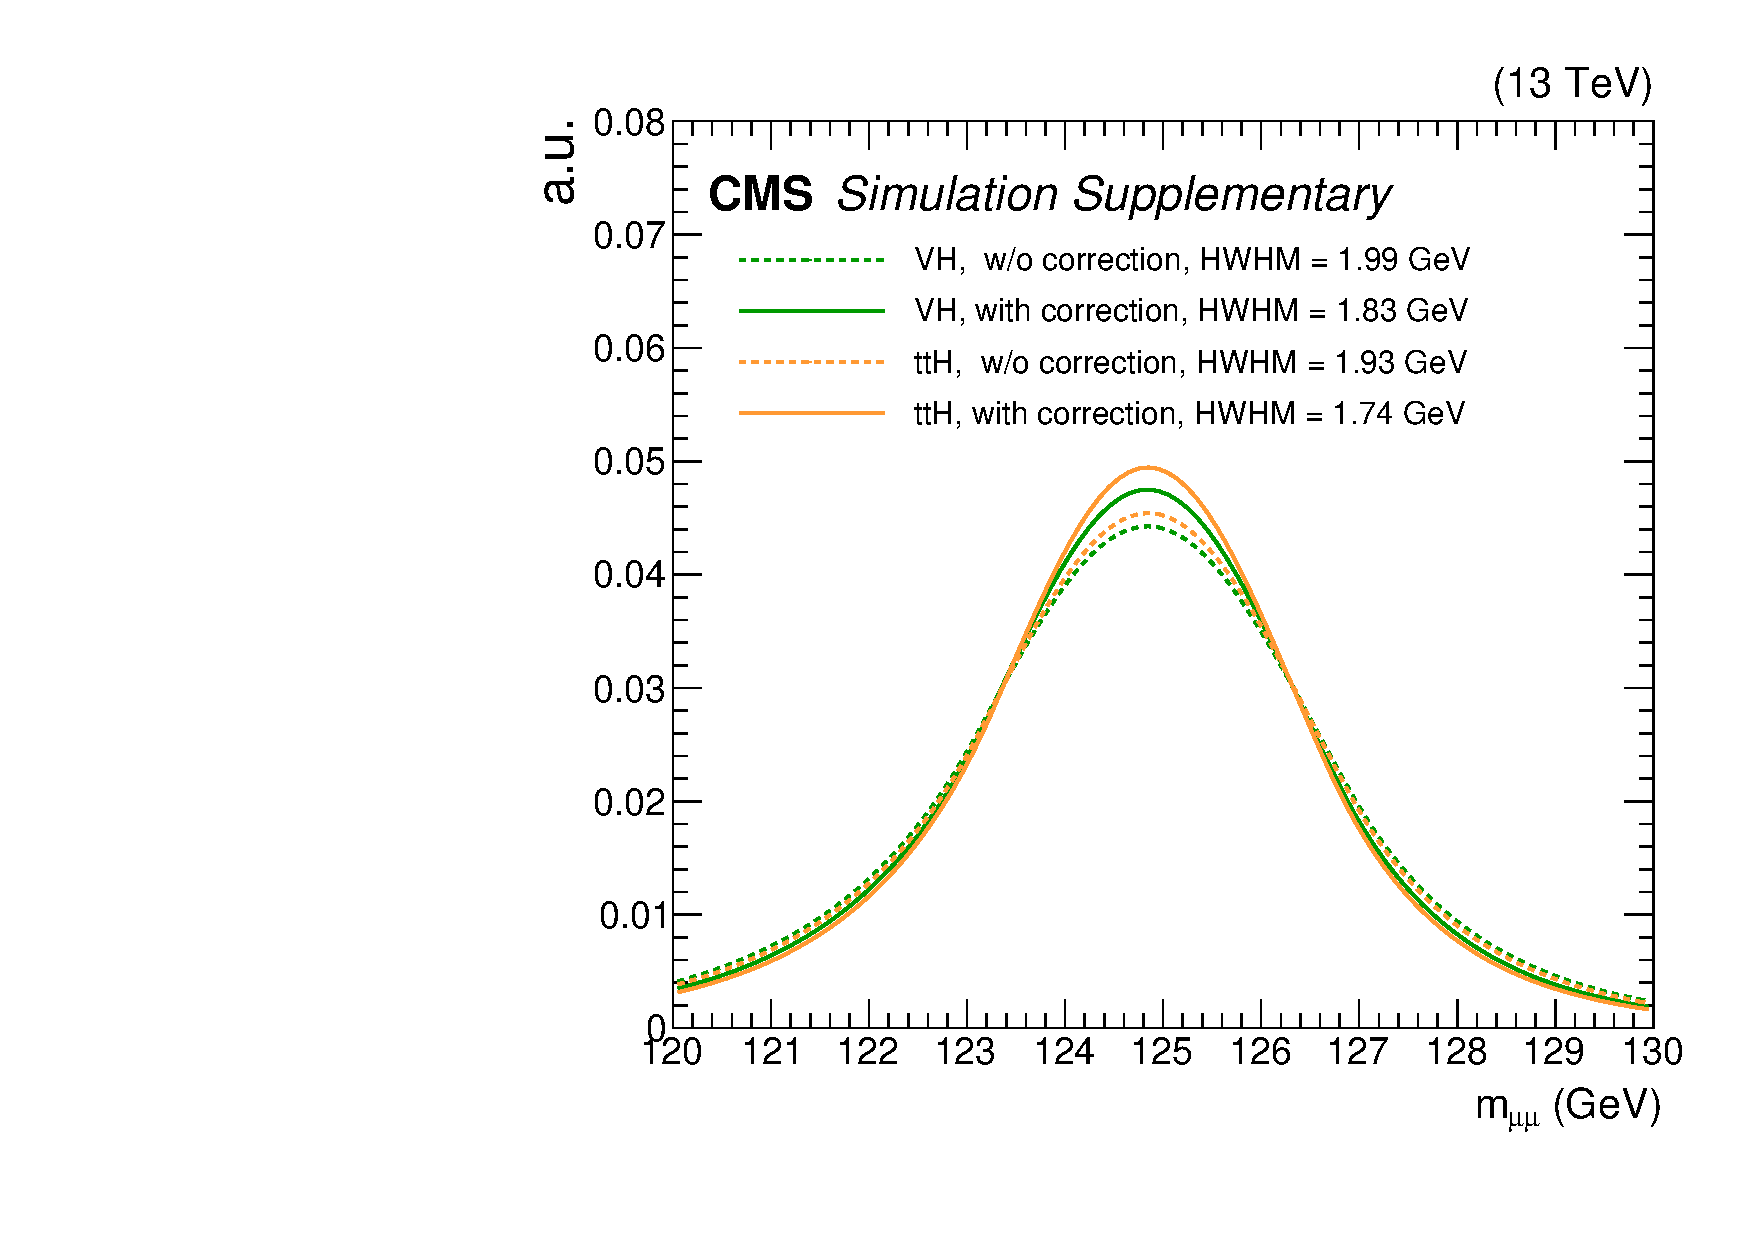
\includegraphics[width=0.45\textwidth]{pics/muon_corr/GeoFit/performance/VHttH.pdf}
      \caption{Plots showing the \GeoFit improvement on the four main \hmm signal modes, 
               \ggH and \qqH plotted on the left, and \VH and \ttH plotted on the right.
               The plots are made combining the expected signal in all three years of data-taking (2016-2018).
               The relative improvements on \mmm resolution for \ggH, \qqH, \VH, and \ttH modes are, respectively,
               6.1\%, 7.8\%, 8.0\%, and 9.8\%.
               }
      \label{fig:geofit_sigs}
\end{figure*}

Overall, the removal of the $\pt-d_0$ dependence leads to an improvement on the inclusive \mmm resolution.
This improvement is different for different processes depending on their kinematic profiles in \pt and |\eta|.
Figure~\ref{fig:geofit_sigs} shows the improvement on \mmm resolution in the four main expected signal modes, \ggH, \qqH, \VH, and \ttH.
The relative improvements on \mmm resolution for \ggH, \qqH, \VH, and \ttH modes are, 
respectively, 6.1\%, 7.8\%, 8.0\%, and 9.8\%.
This improvement on signal resolution translates to about 5\% improvement on the significance of the inclusive \hmm analysis.

The different improvements in different signal modes comes from their \pt profiles.
As the correction is proportional to $d_0$ and $\pt^{2}$, 
the relative improvement $\Delta\pt / \pt$ is proportional to $d_0$ and \pt. 
Figure~\ref{fig:sigs_d0_pt} shows the $d_0$ (left) and \pt (right) distributions of different signal modes.
The $d_0$ profiles of the 4 signals are exactly the same,
while the \pt profiles are different.
\ttH signal has more high \pt muons than other signal modes,
while \ggH signal has more muons on the low \pt side.
Therefore they gain the largest and smallest improvements from the \GeoFit, respectively.
\qqH and \VH signals have very similar \pt profiles, 
and their improvements from the \GeoFit are about the same.

\begin{figure*}[!htb]
      \centering
      \captionsetup{justification=justified}
      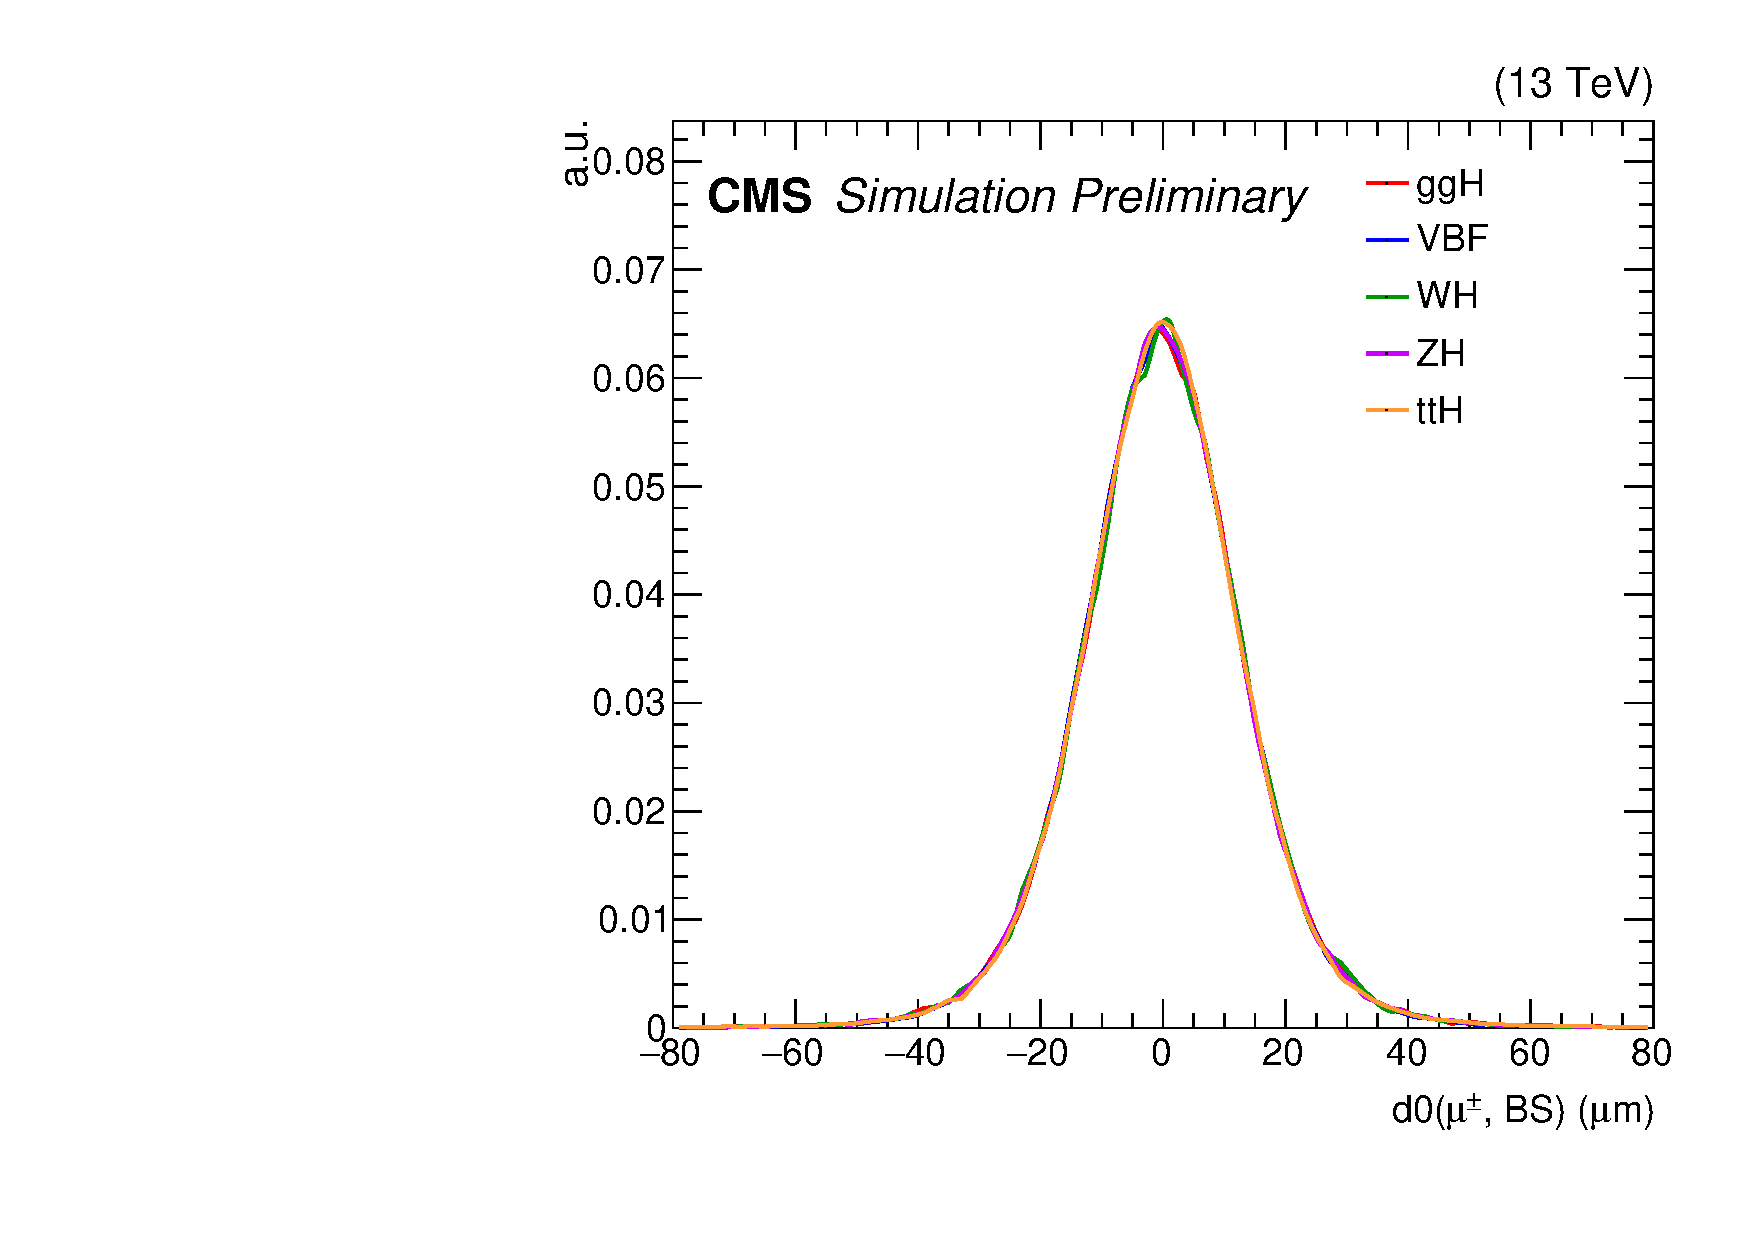
\includegraphics[width=0.45\textwidth]{pics/muon_corr/GeoFit/performance/samp_d0.pdf}
      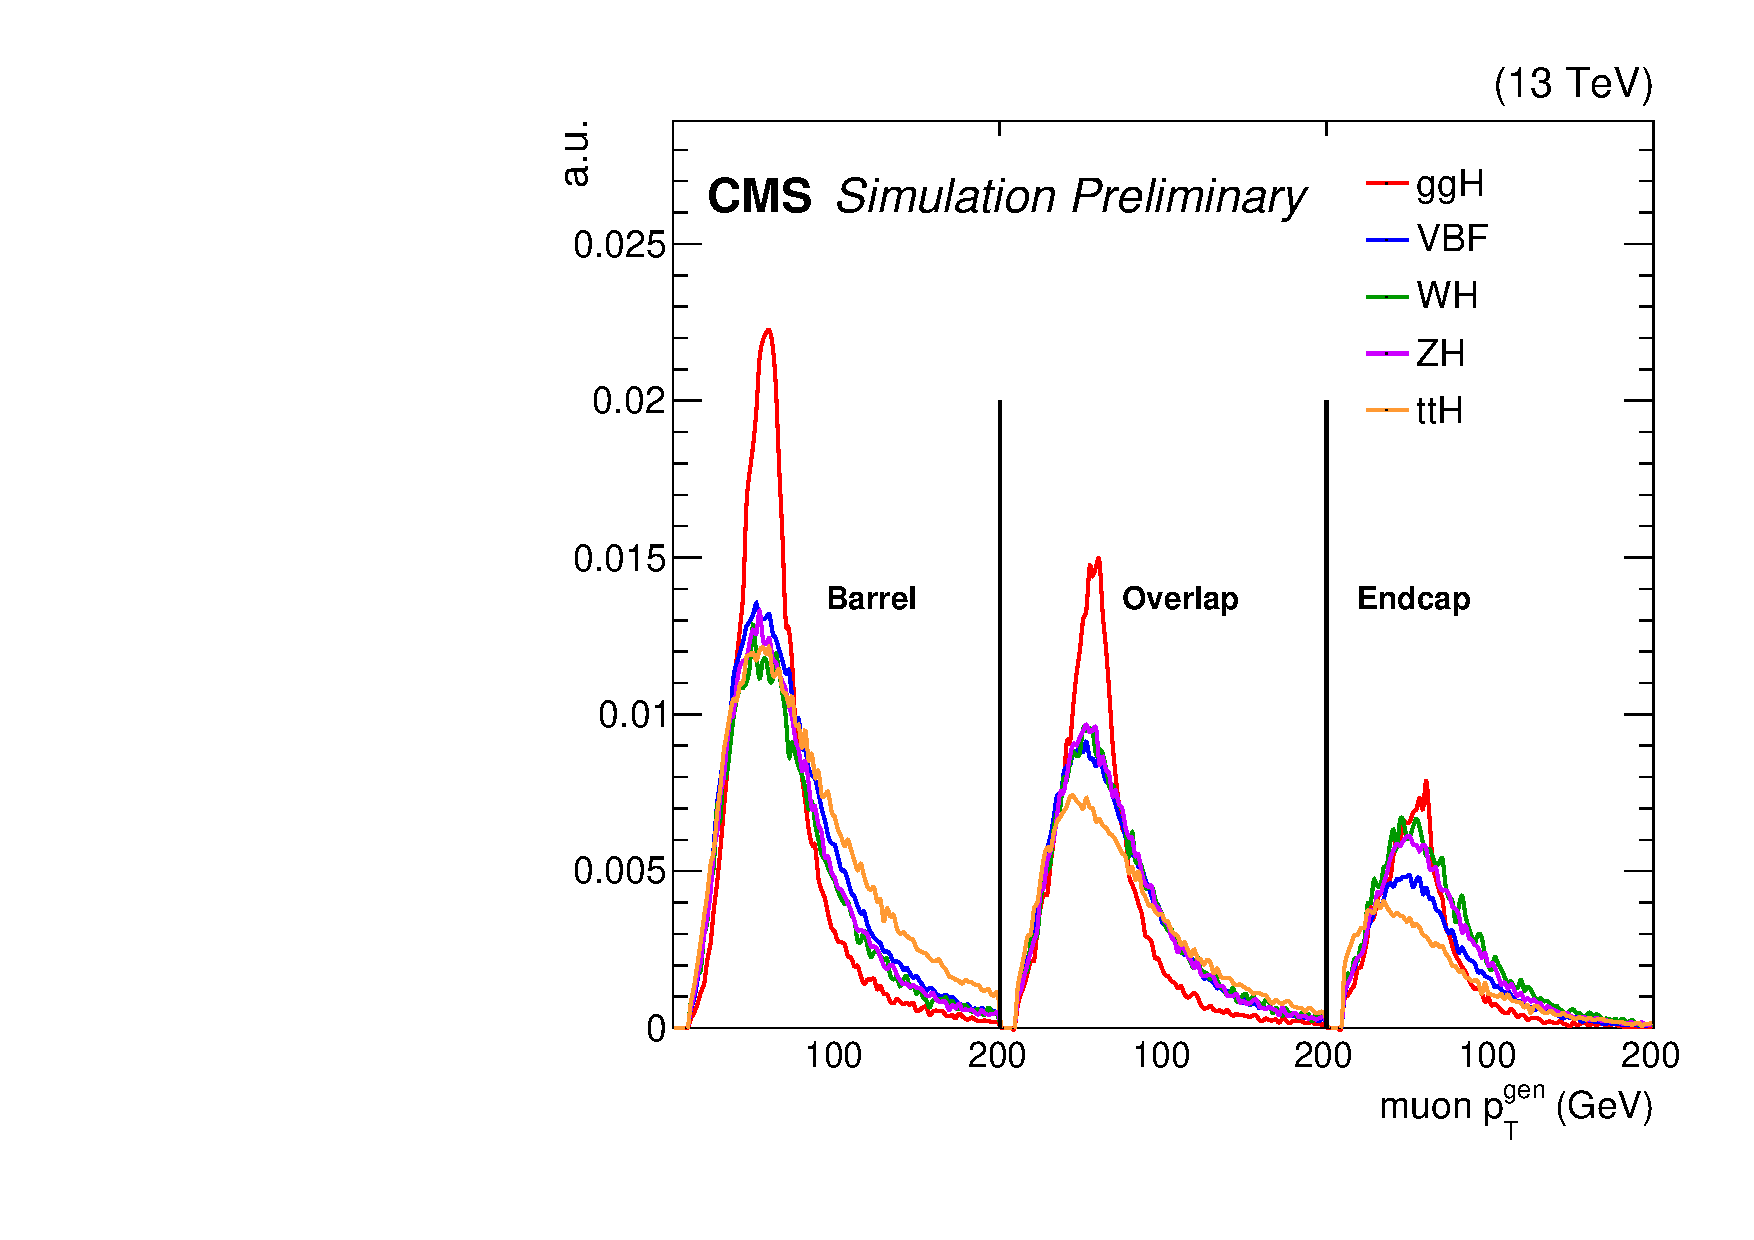
\includegraphics[width=0.45\textwidth]{pics/muon_corr/GeoFit/performance/samp_pt_BOE.pdf}
      \caption{Plots showing $d_0$ and \pt distributions of the four main \hmm signal modes. 
               The $d_0$ profiles (left plot) of the 4 signals are the same.
               The \pt profiles (right plot) are different, which explains the different relative improvements  
               that the signals receive from the \GeoFit.
               }
      \label{fig:sigs_d0_pt}
\end{figure*}



\subsection{GeoFit vs track refit}\label{sec:track_refit}

The \GeoFit provides a simple method to correct the \pt dependence on d0 based on high level physics variables.
Since the origin of this \pt dependence is well-understood, it is also possible to derive a more fundamental correction
by refitting each muon track including the BS position as an additional constraint to the track.
This method requires lower-level information of muon reconstruction and is computationally more expensive,
but is in principle more precise.
To compare the performance of the \GeoFit and the refit method, a preliminary study is made on the 2018 \ggH signal simulation.
The \mmm shape of the inclusive signal is plotted applying the track refit method vs applying the \GeoFit, shown in Figure~\ref{fig:refit_vs_geofit}.
This comparison shows that the \mmm shapes from the two methods are almost equivalent.
The \GeoFit, although an approximation method, captures most of the effect and provides about the same improvement in \mmm resolution as the refit method.
The \GeoFit is therefore chosen in the \hmm analysis to speed up the workflow.

\begin{figure*}[!htb]
      \centering
      \captionsetup{justification=justified}
      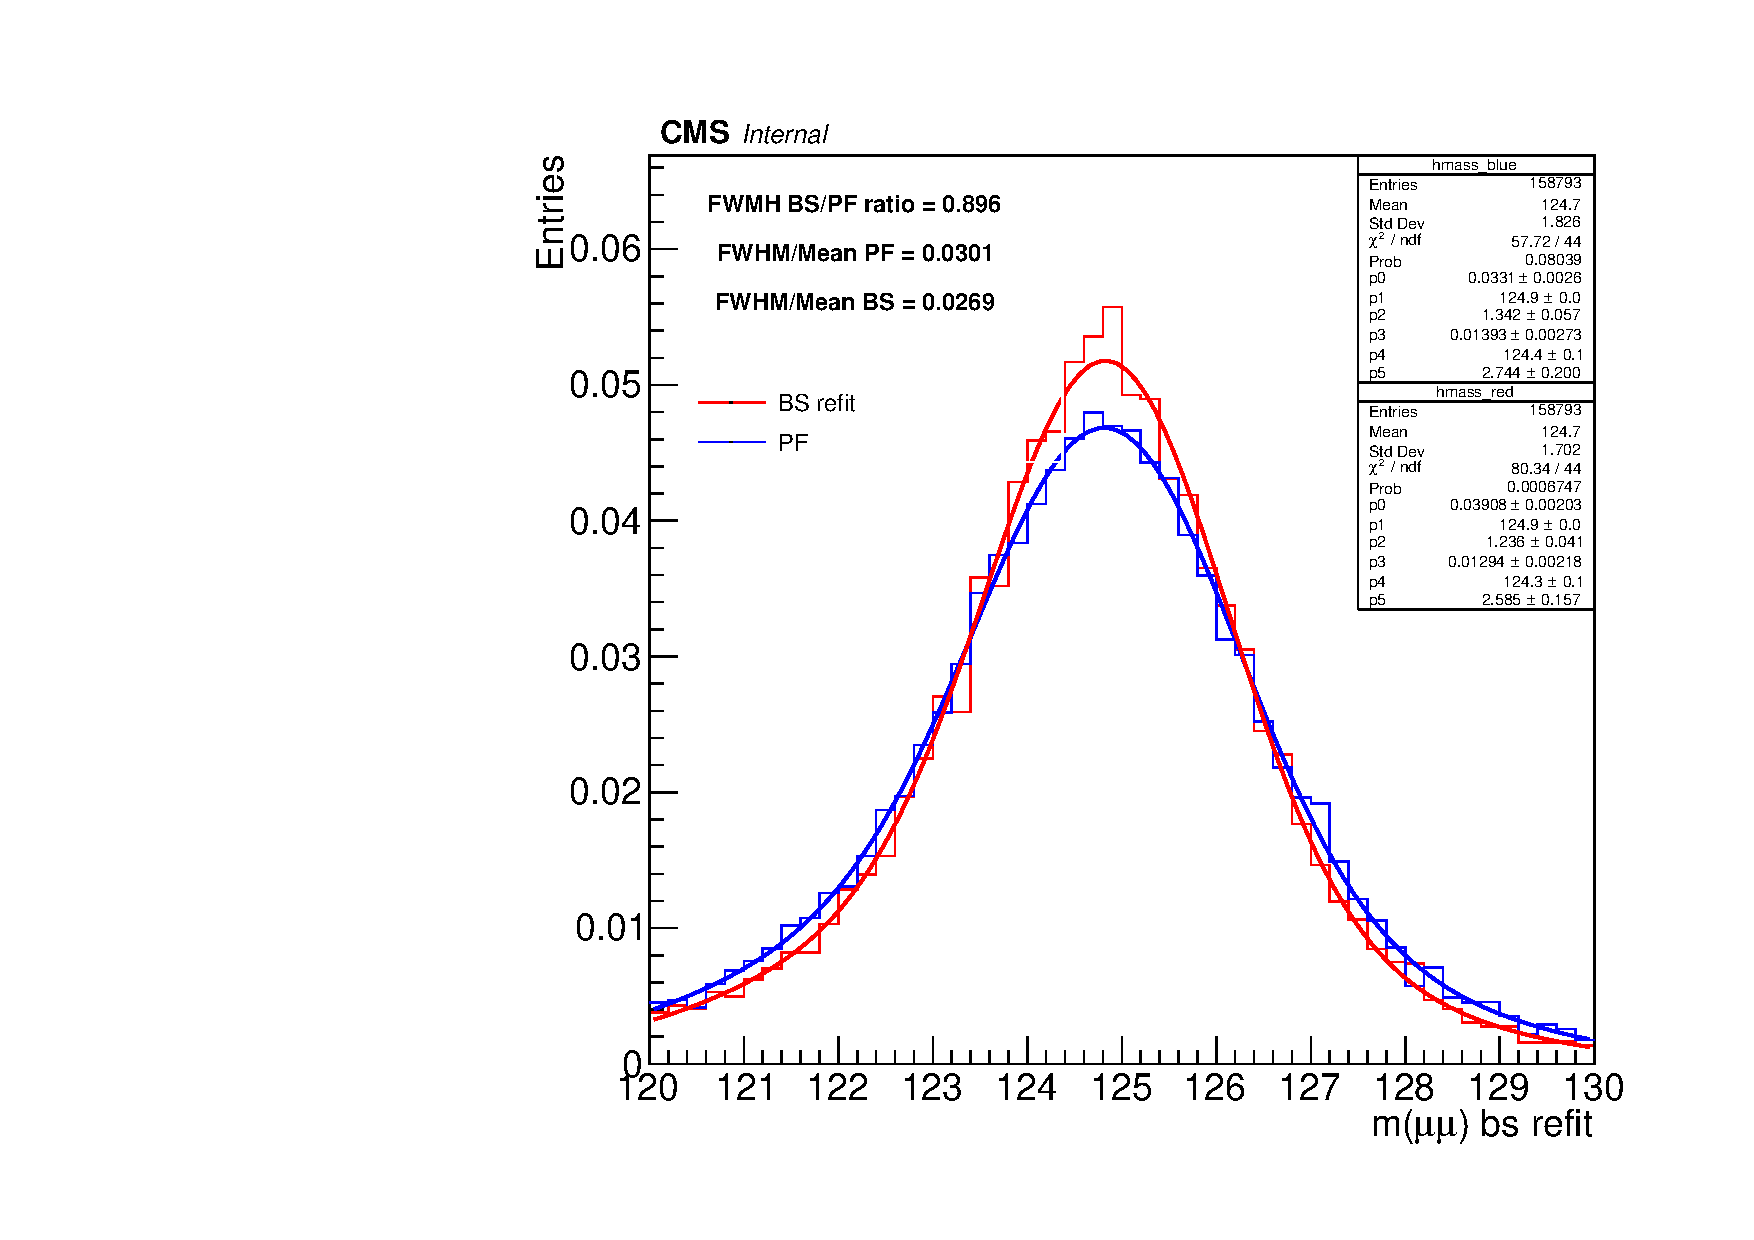
\includegraphics[width=0.45\textwidth]{pics/muon_corr/GeoFit/track_refit/ggH_mass_muon_fit_bs_pf_2018.pdf}
      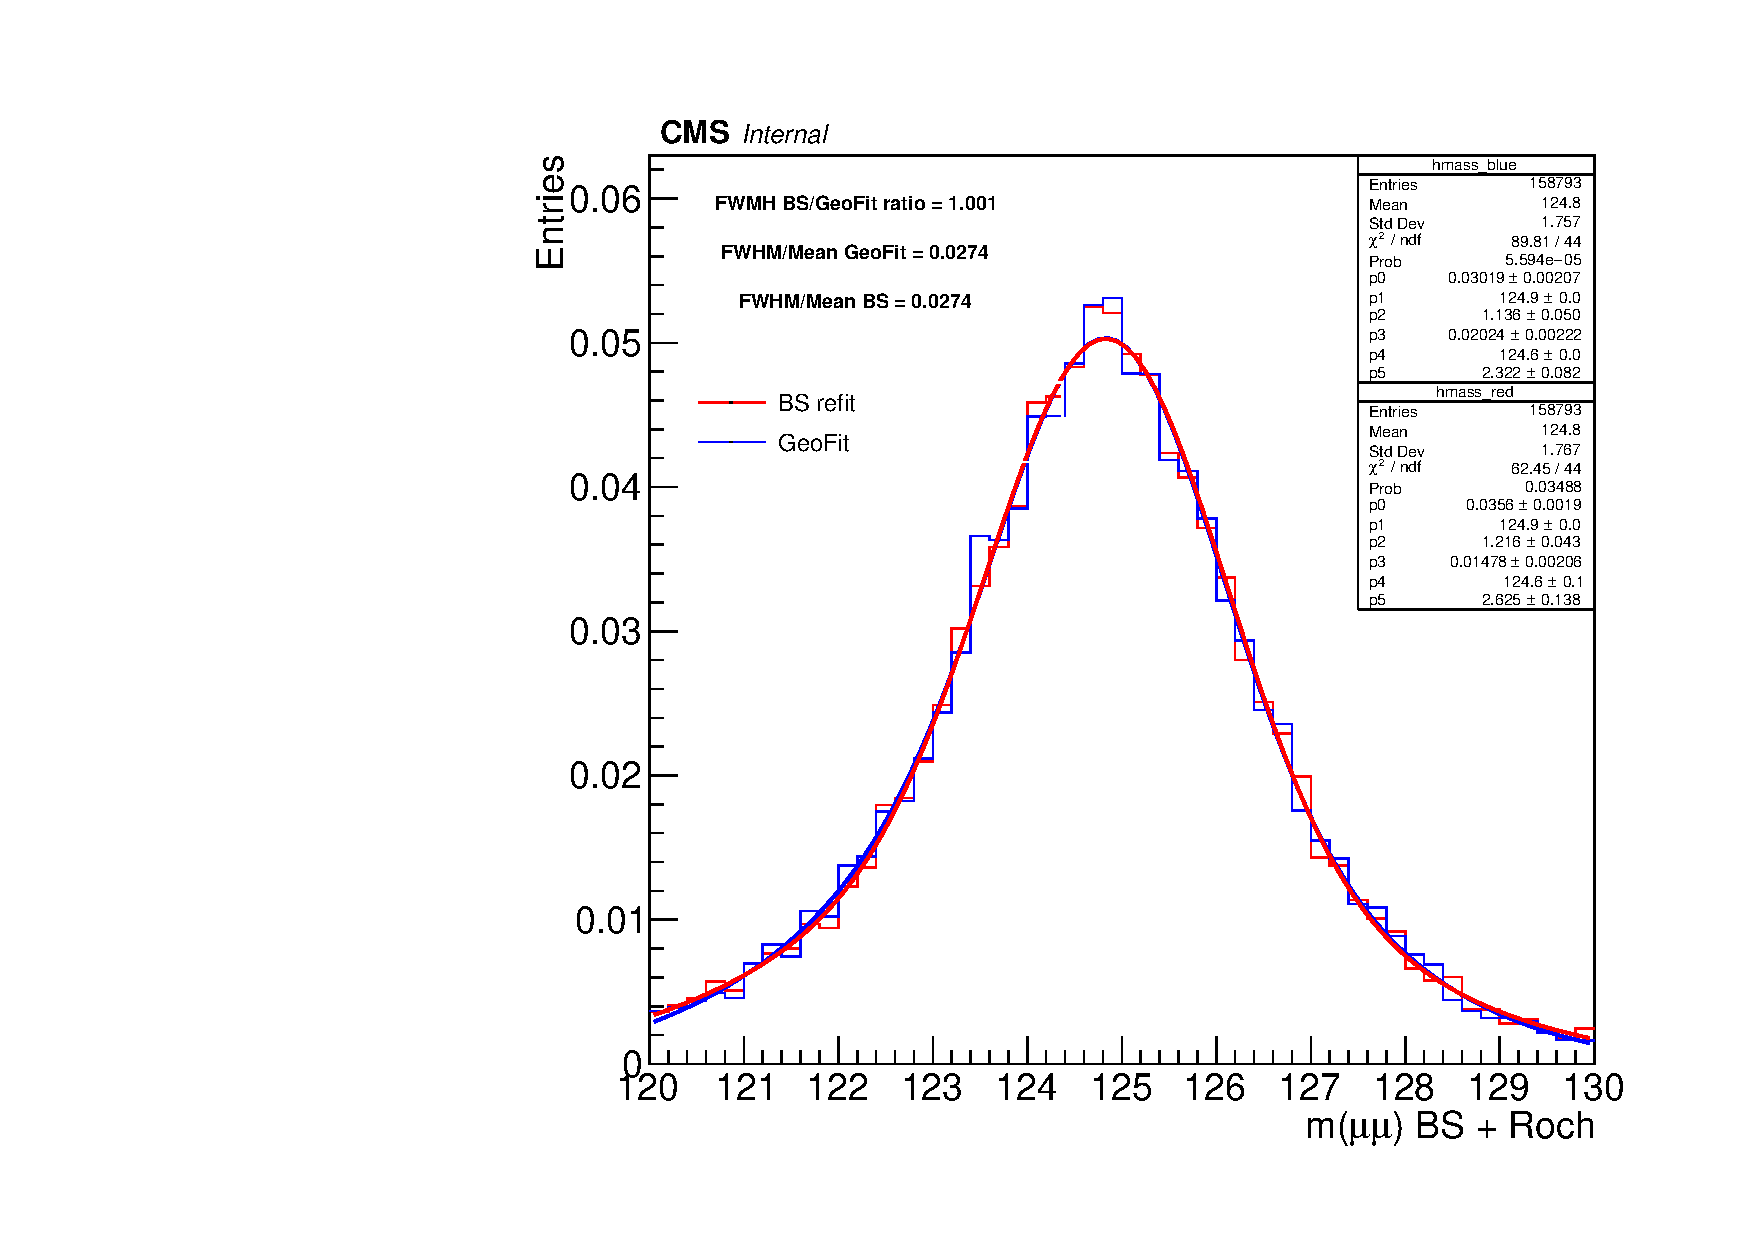
\includegraphics[width=0.45\textwidth]{pics/muon_corr/GeoFit/track_refit/ggH_mass_muon_fit_bs_geofit_2018.pdf}
      \caption{Plots of the \mmm shape of the 2018 \ggH simulation sample, comparing different muon correction methods.
               The left plot shows the \mmm distribution calculated with muon tracks refitted with the additional BS constraint, 
               compared with the particle flow shape (left plot).
               The \RochCorr is not applied in the left plot for both the red and the blue lines.
               The right plot shows the \mmm distribution from the refit method, with the \RochCorr applied,
               compared with the shape from \GeoFit + \RochCorr (right plot).
               Plots credit to Pierluigi Bortignon.}
      \label{fig:refit_vs_geofit}
\end{figure*}

\section{Muon calibration results} \label{sec:muon_cal}

The \zmm is a well-understood process with a mass scale not far from the Higgs boson and with a much larger number of events at the LHC.
It is therefore used as a candle to monitor the performance of the \RochCorr and the \GeoFit, 
and validate that these corrections do not introduce new biases.
In this study, the distribution of the \mmm is plotted in different bins of various dimuon kinematic variables.
The \mmm distributions are fit with a Voigtian + Exponential function, 
in which the Voigtian part is a convolution of a Breit-Wigner function and a Gaussian function.
The parameter "mean mass" from the Breit-Wigner part and standard deviation from the Gaussian part are 
taken as the mean value and the experimental resolution of the \mmm distribution.
They are plotted against the dimuon kinematic variable of interest to check for potential trends.

The calibration plots are made by year as the corrections are provided by year.
Events containing \FSR are removed from this study as it is a separate effect.
Different variables are tested in the Figures listed: 
Figure~\ref{fig:mucal_muP_eta} for the \eta ~of the positive muon,
Figure~\ref{fig:mucal_muP_phi} for the \phi ~of the positive muon,
Figure~\ref{fig:mucal_muN_phi} for the \phi ~of the negative muon,
Figure~\ref{fig:mucal_muP_pt} for the \pt ~of the positive muon,
Figure~\ref{fig:mucal_dimu_pt} for the \pt ~of the dimuon system,
Figure~\ref{fig:mucal_dimu_eta} for the \eta ~of the dimuon system,
Figure~\ref{fig:mucal_muP_d0} for the $d_0$ of the positive muon,
and Figure~\ref{fig:mucal_muN_d0} for the $d_0$ of the negative muon.

From these plots, it can be concluded that all the known biases in muon \pt are removed and no new bias has been introduced.
The \RochCorr and \GeoFit correct orthogonal effects, and do not interfere with the performance of each other.
After the corrections, a per-mille level agreement is achieved between data and simulation in the \mmm value,
while the agreement in \mmm resolution is about a few percent. 

\begin{figure*}[!htb]
      \centering
      \captionsetup{justification=justified}
      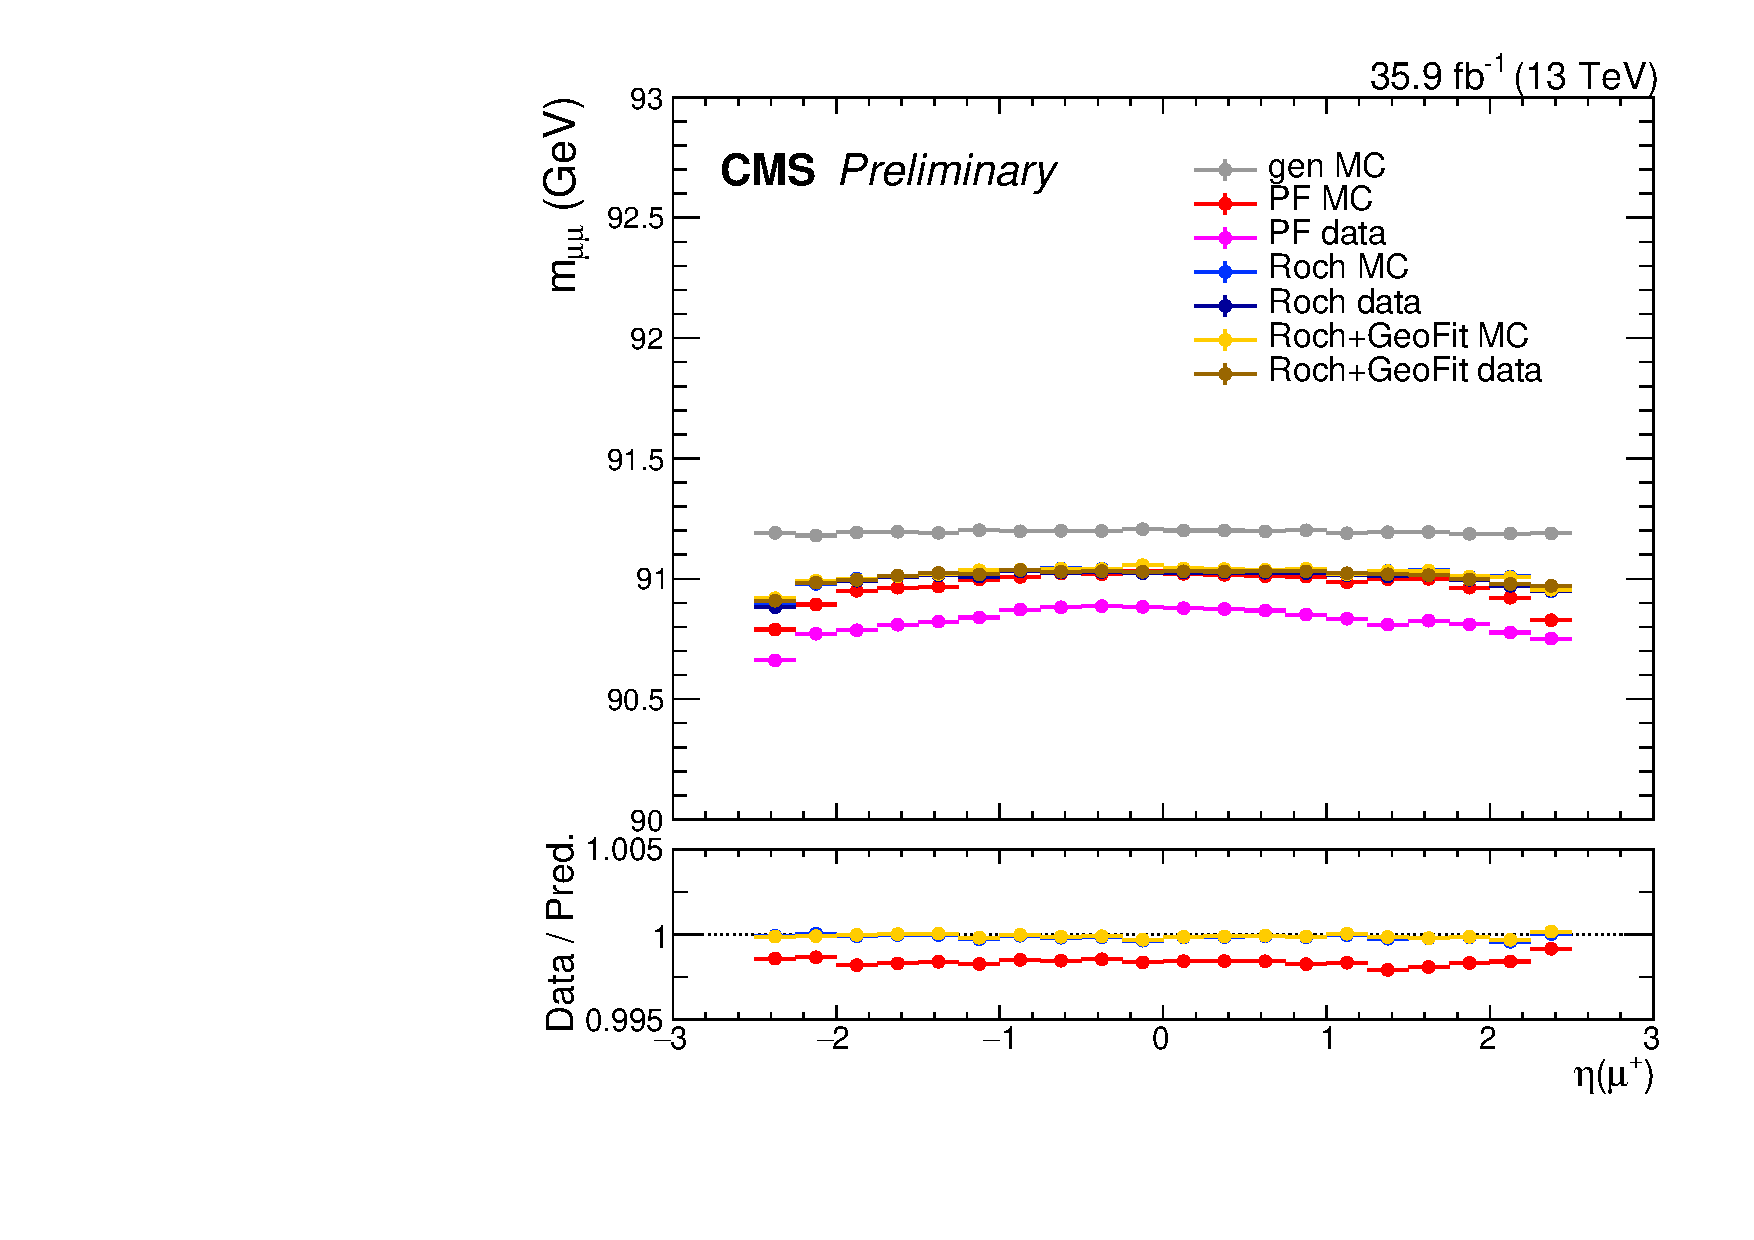
\includegraphics[width=0.32\textwidth]{pics/muon_corr/muon_cal/2016/muP_eta_summary_mean.pdf}
      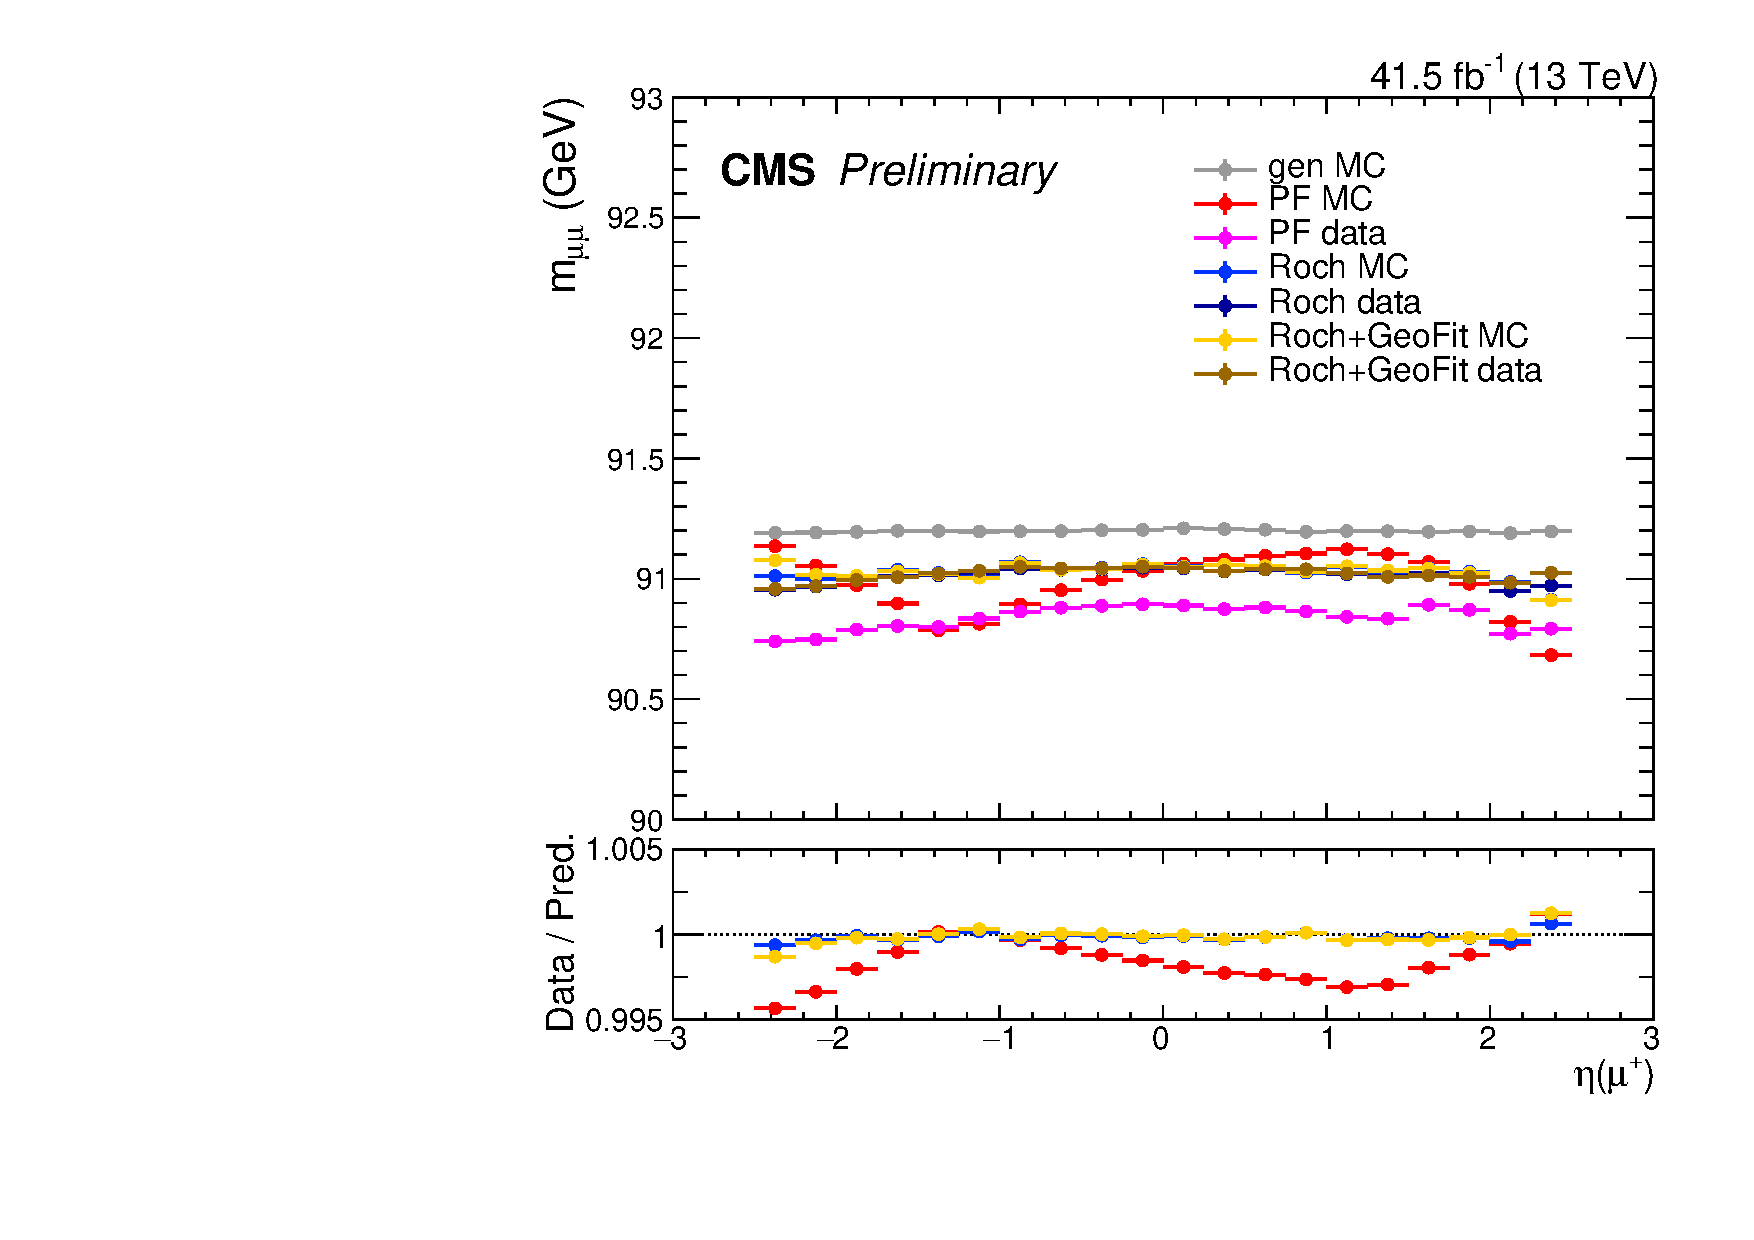
\includegraphics[width=0.32\textwidth]{pics/muon_corr/muon_cal/2017/muP_eta_summary_mean.pdf}
      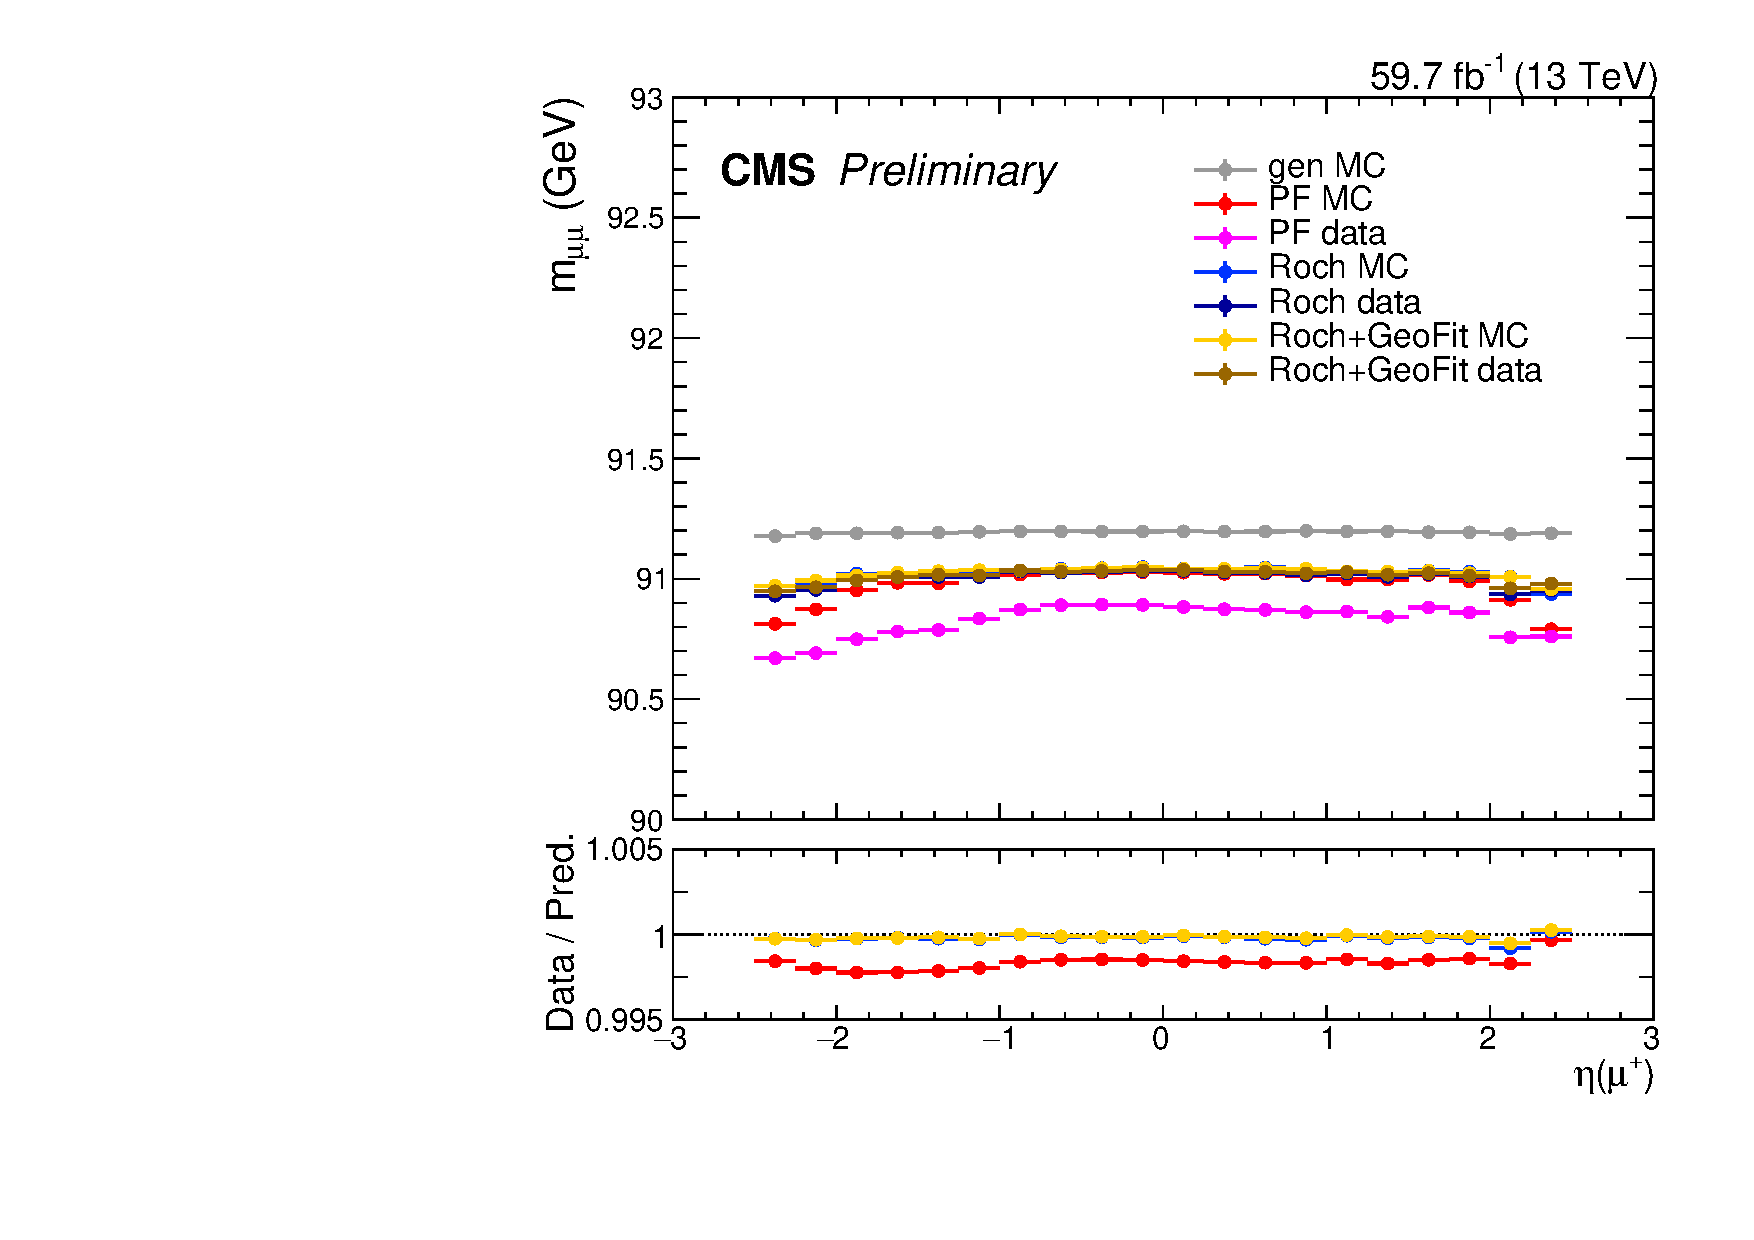
\includegraphics[width=0.32\textwidth]{pics/muon_corr/muon_cal/2018/muP_eta_summary_mean.pdf}
      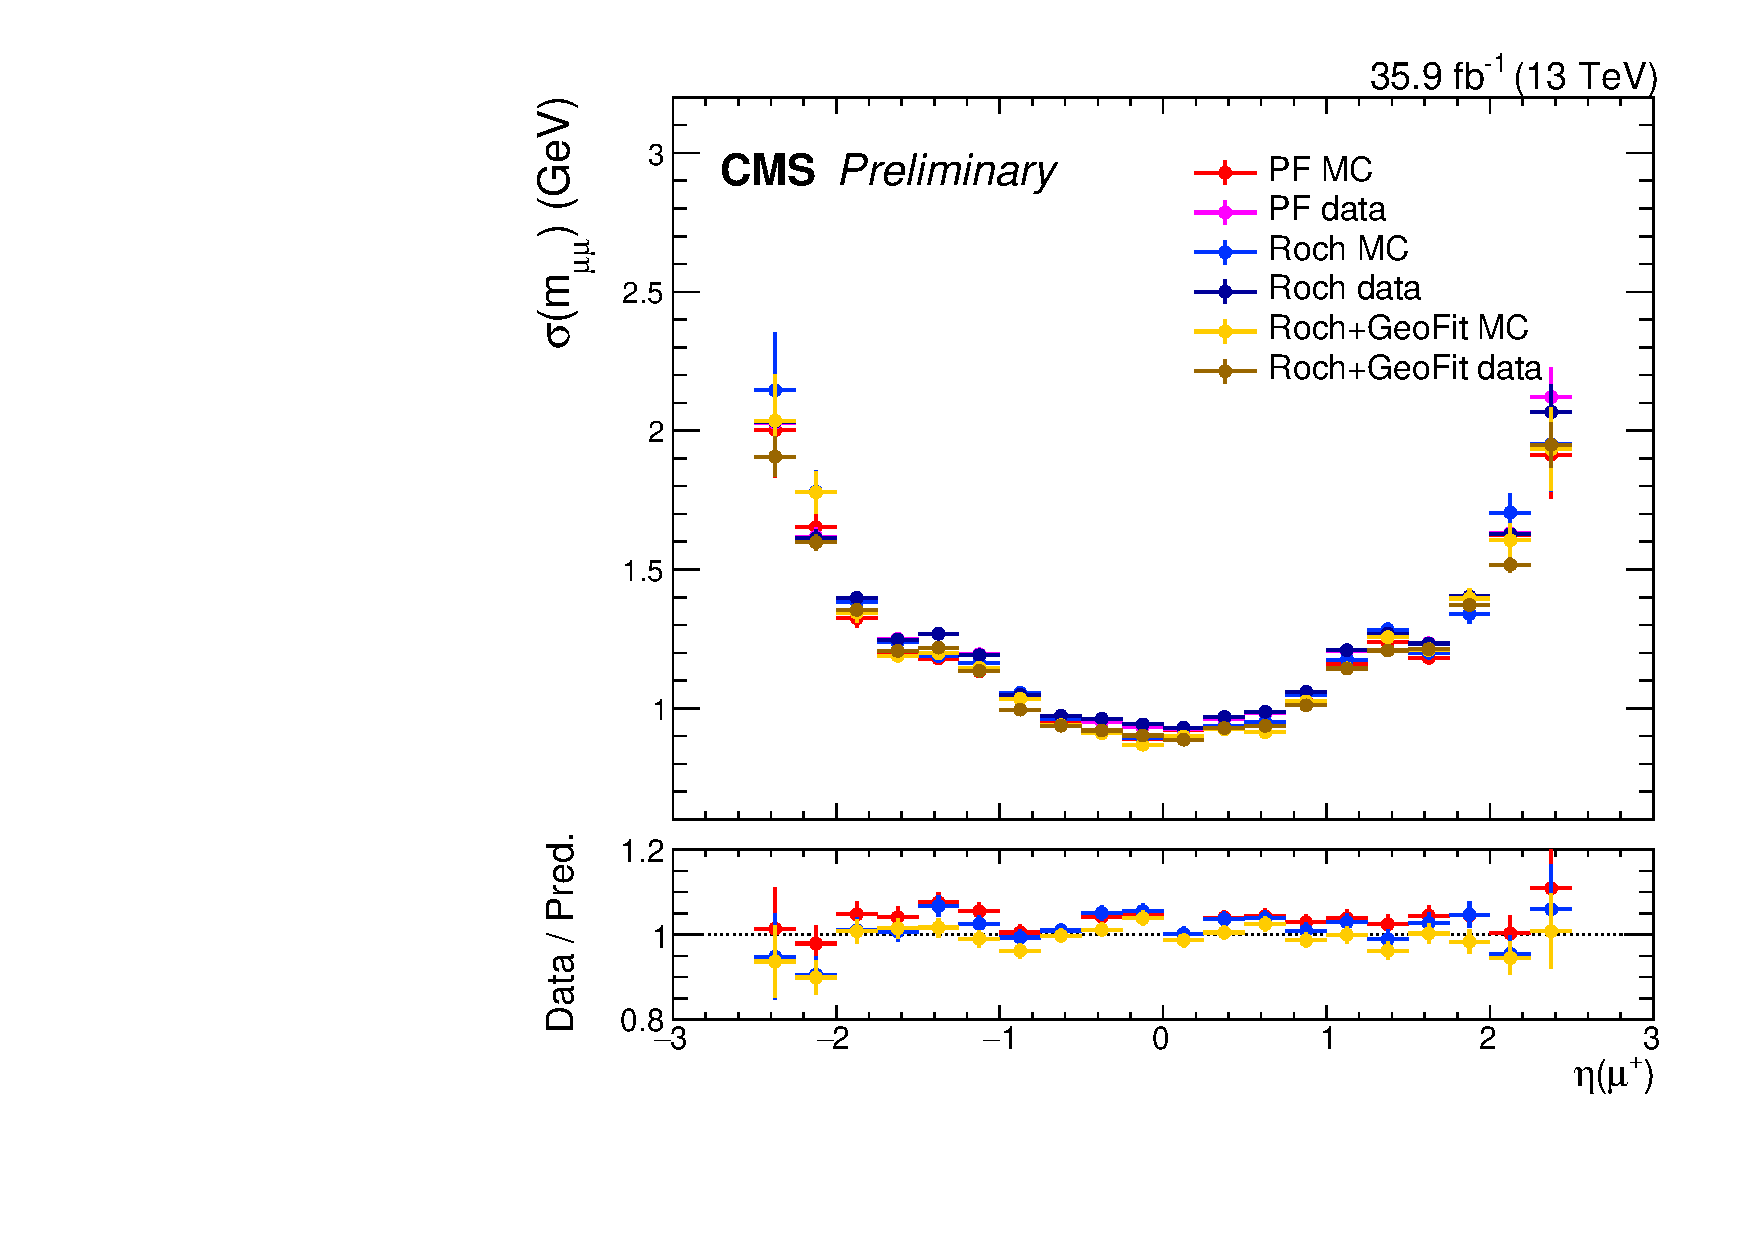
\includegraphics[width=0.32\textwidth]{pics/muon_corr/muon_cal/2016/muP_eta_summary_reso.pdf}
      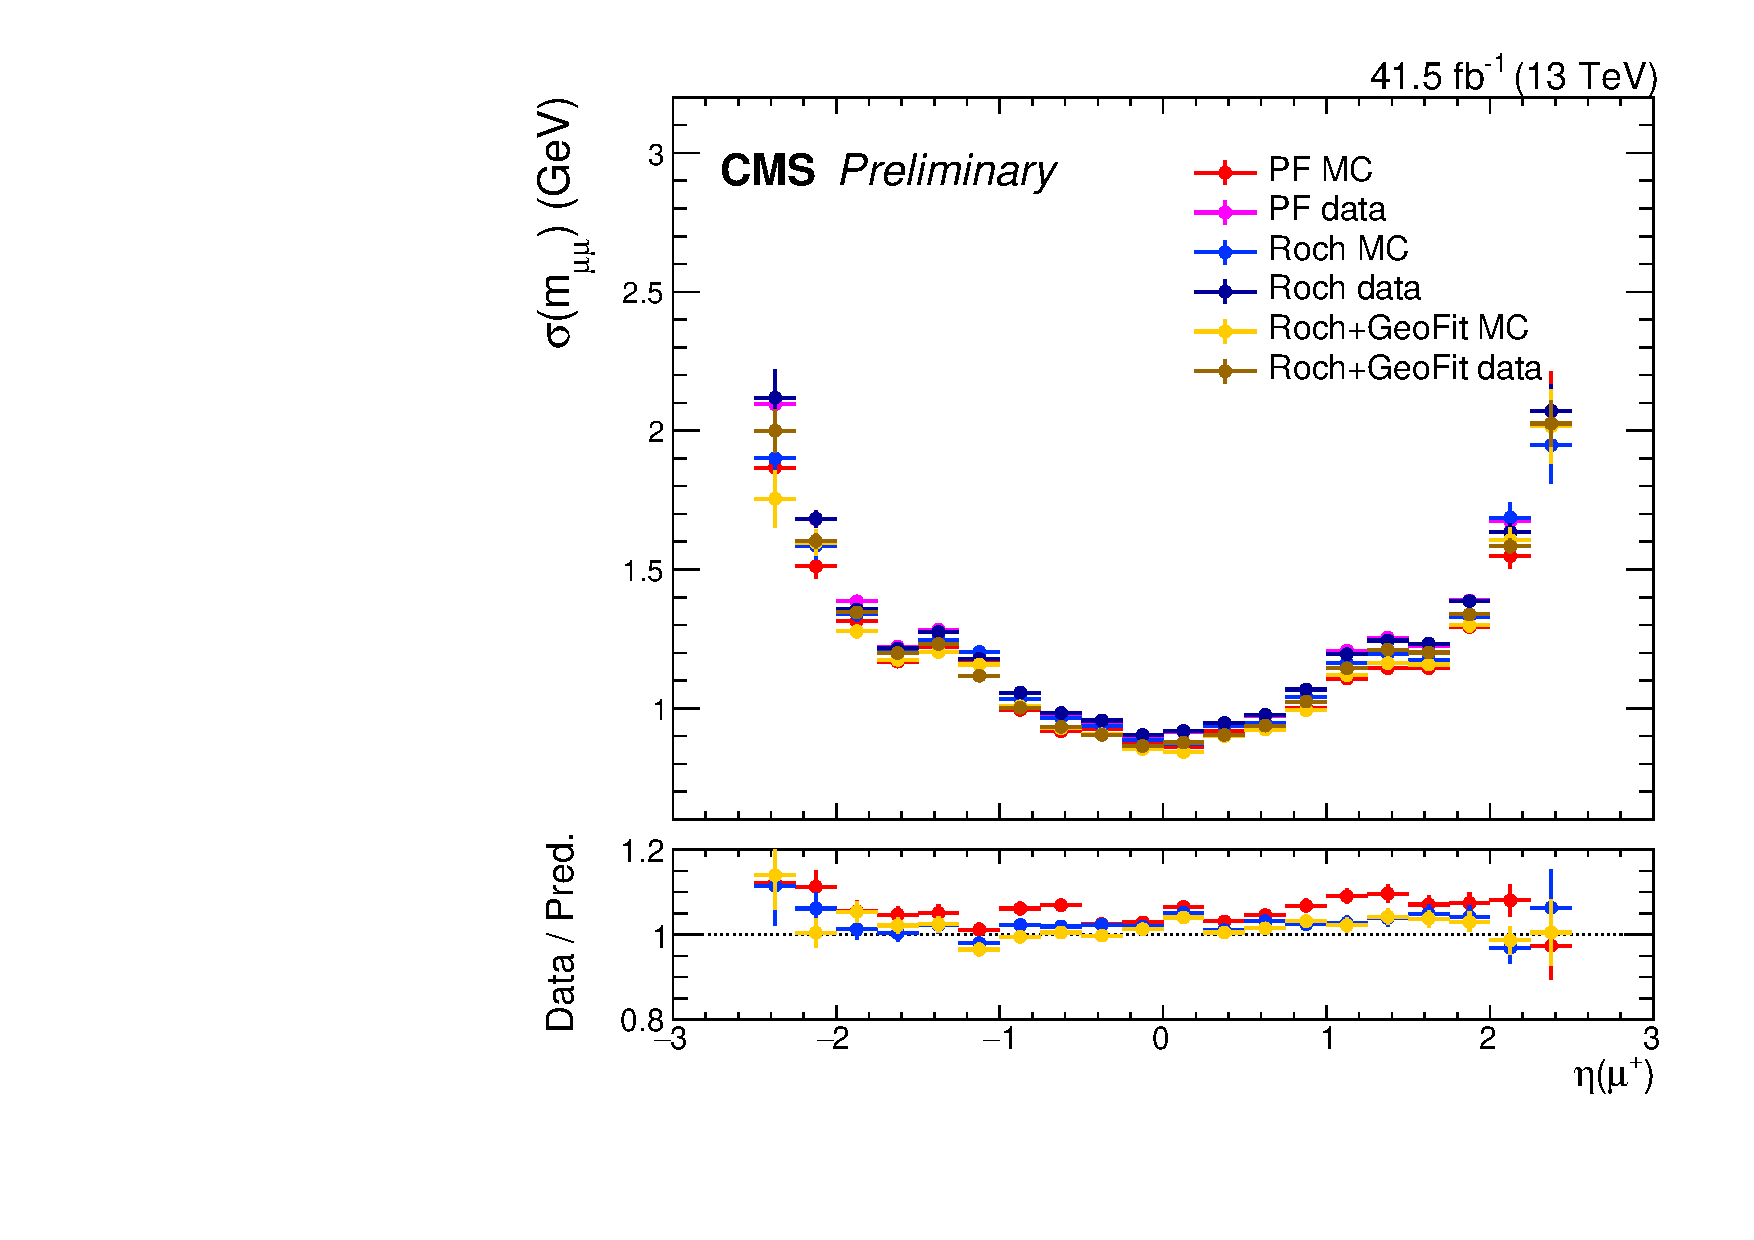
\includegraphics[width=0.32\textwidth]{pics/muon_corr/muon_cal/2017/muP_eta_summary_reso.pdf}
      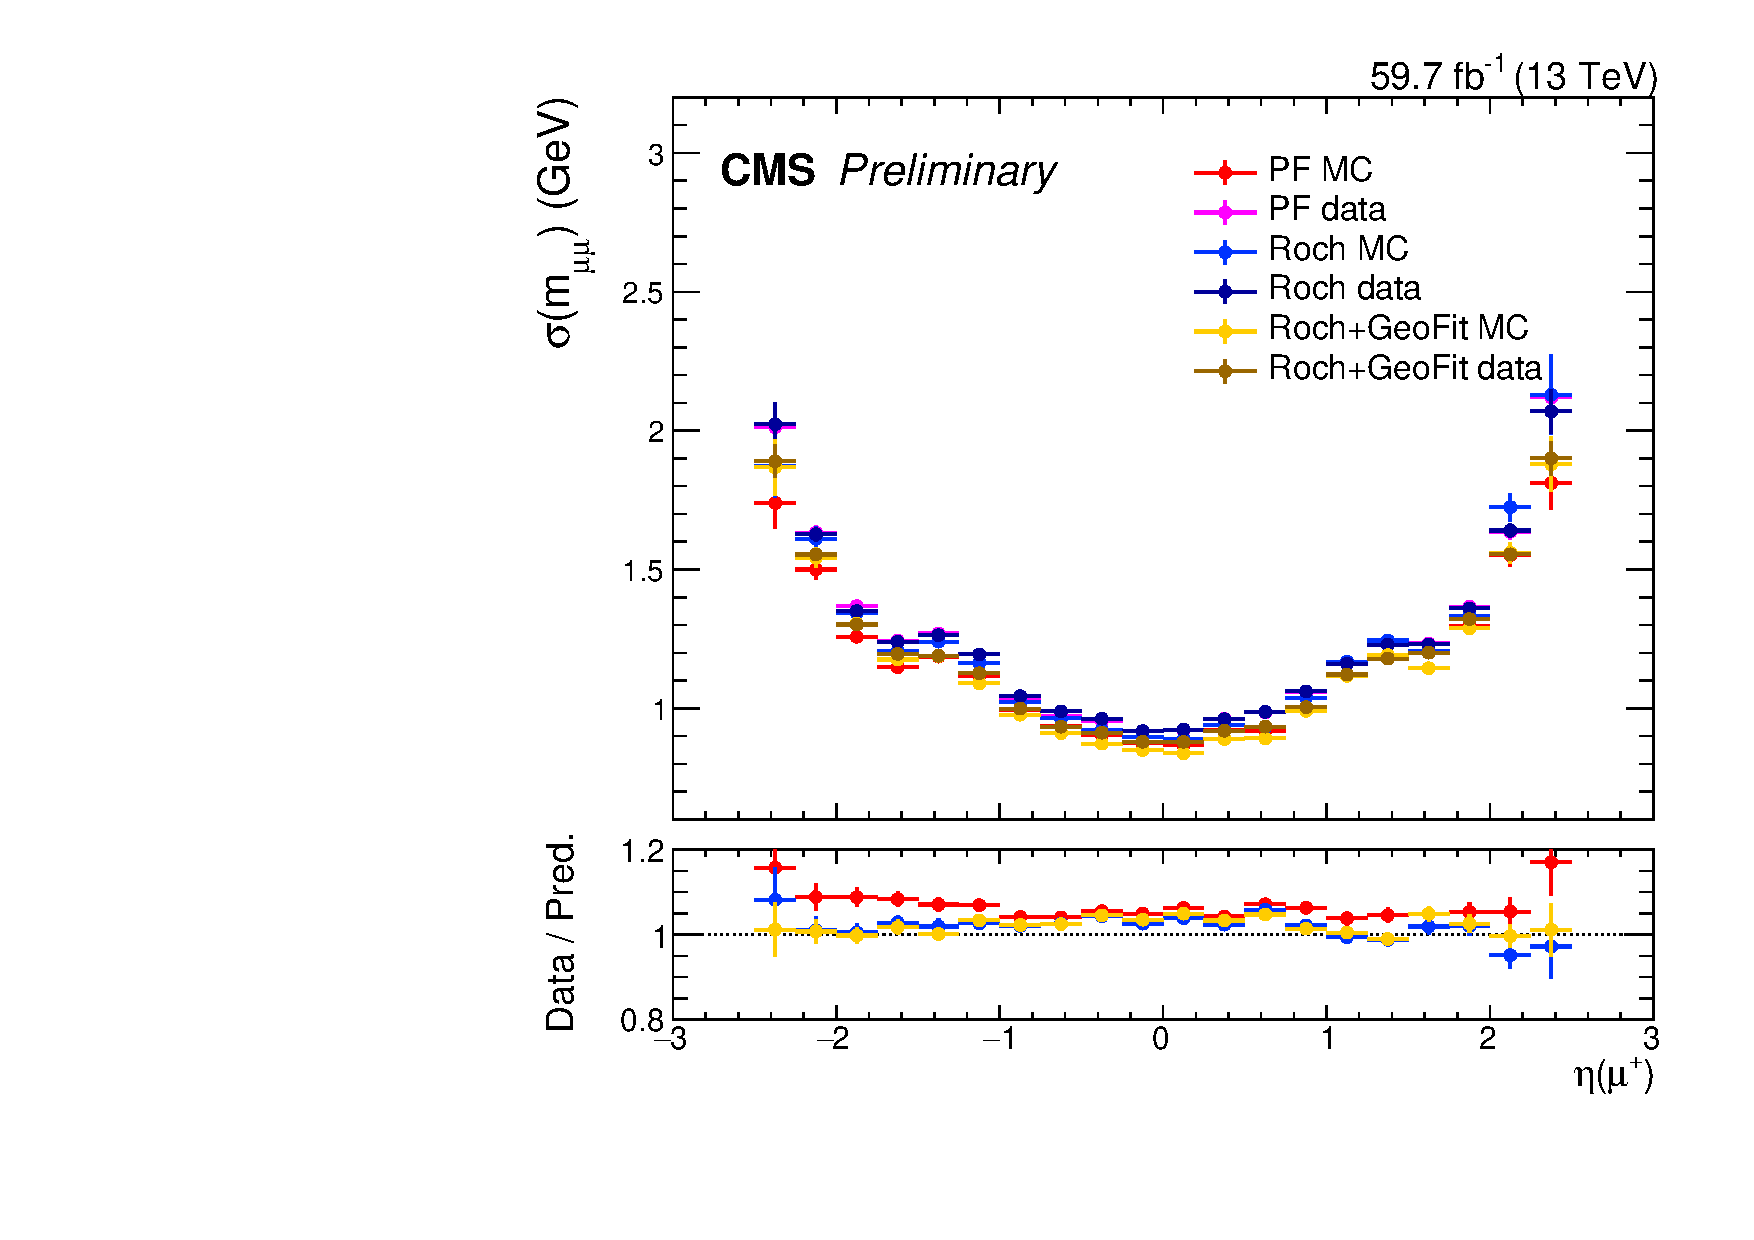
\includegraphics[width=0.32\textwidth]{pics/muon_corr/muon_cal/2018/muP_eta_summary_reso.pdf}
      \caption{Muon calibration plots vs $\eta(\mu^{+})$, for 2016 (left column), 2017 (middle column) and 2018 (right column).
               The top row shows the mean value of the Voigtian fit to the \mmm distribution, 
               while the bottom row shows its experimental resolution.}
      \label{fig:mucal_muP_eta}
\end{figure*}


\begin{figure*}[!htb]
      \centering
      \captionsetup{justification=justified}
      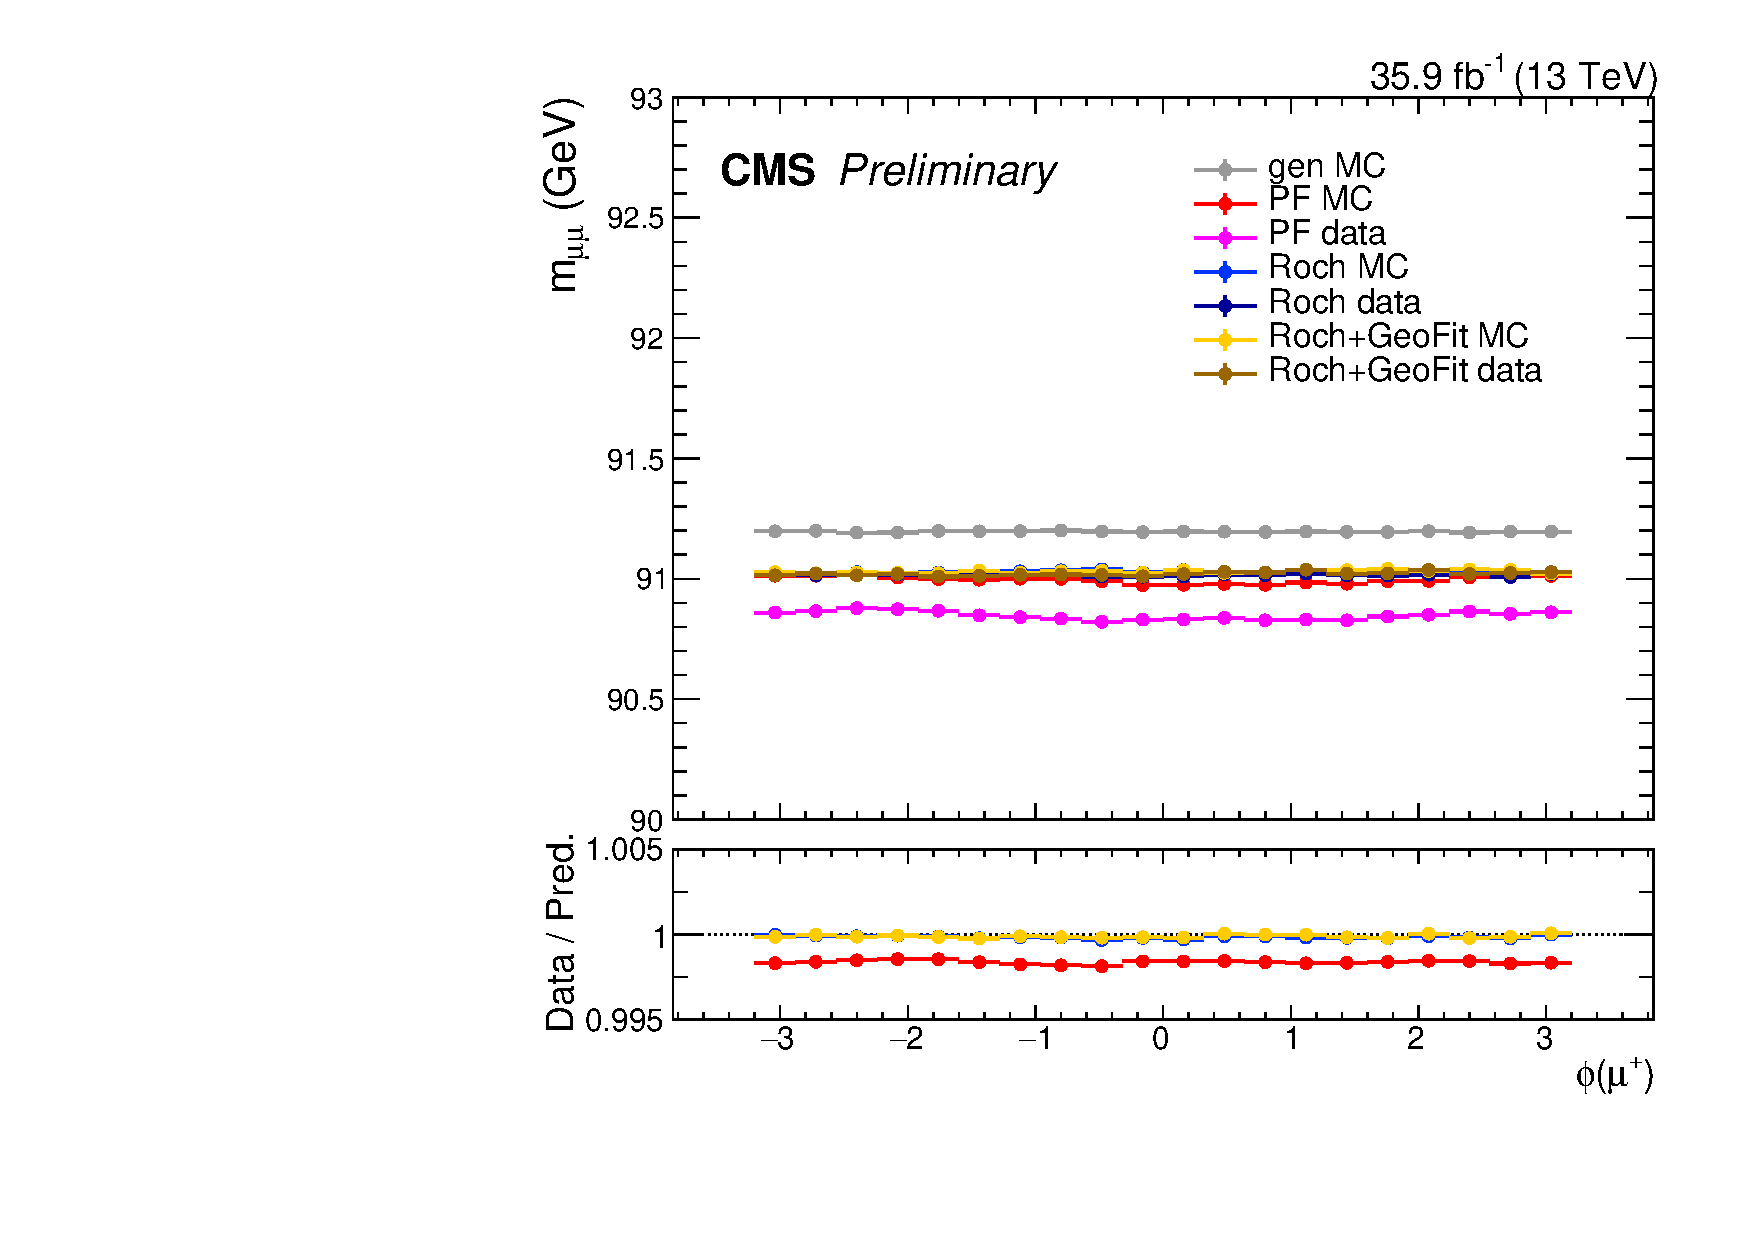
\includegraphics[width=0.32\textwidth]{pics/muon_corr/muon_cal/2016/muP_phi_summary_mean.pdf}
      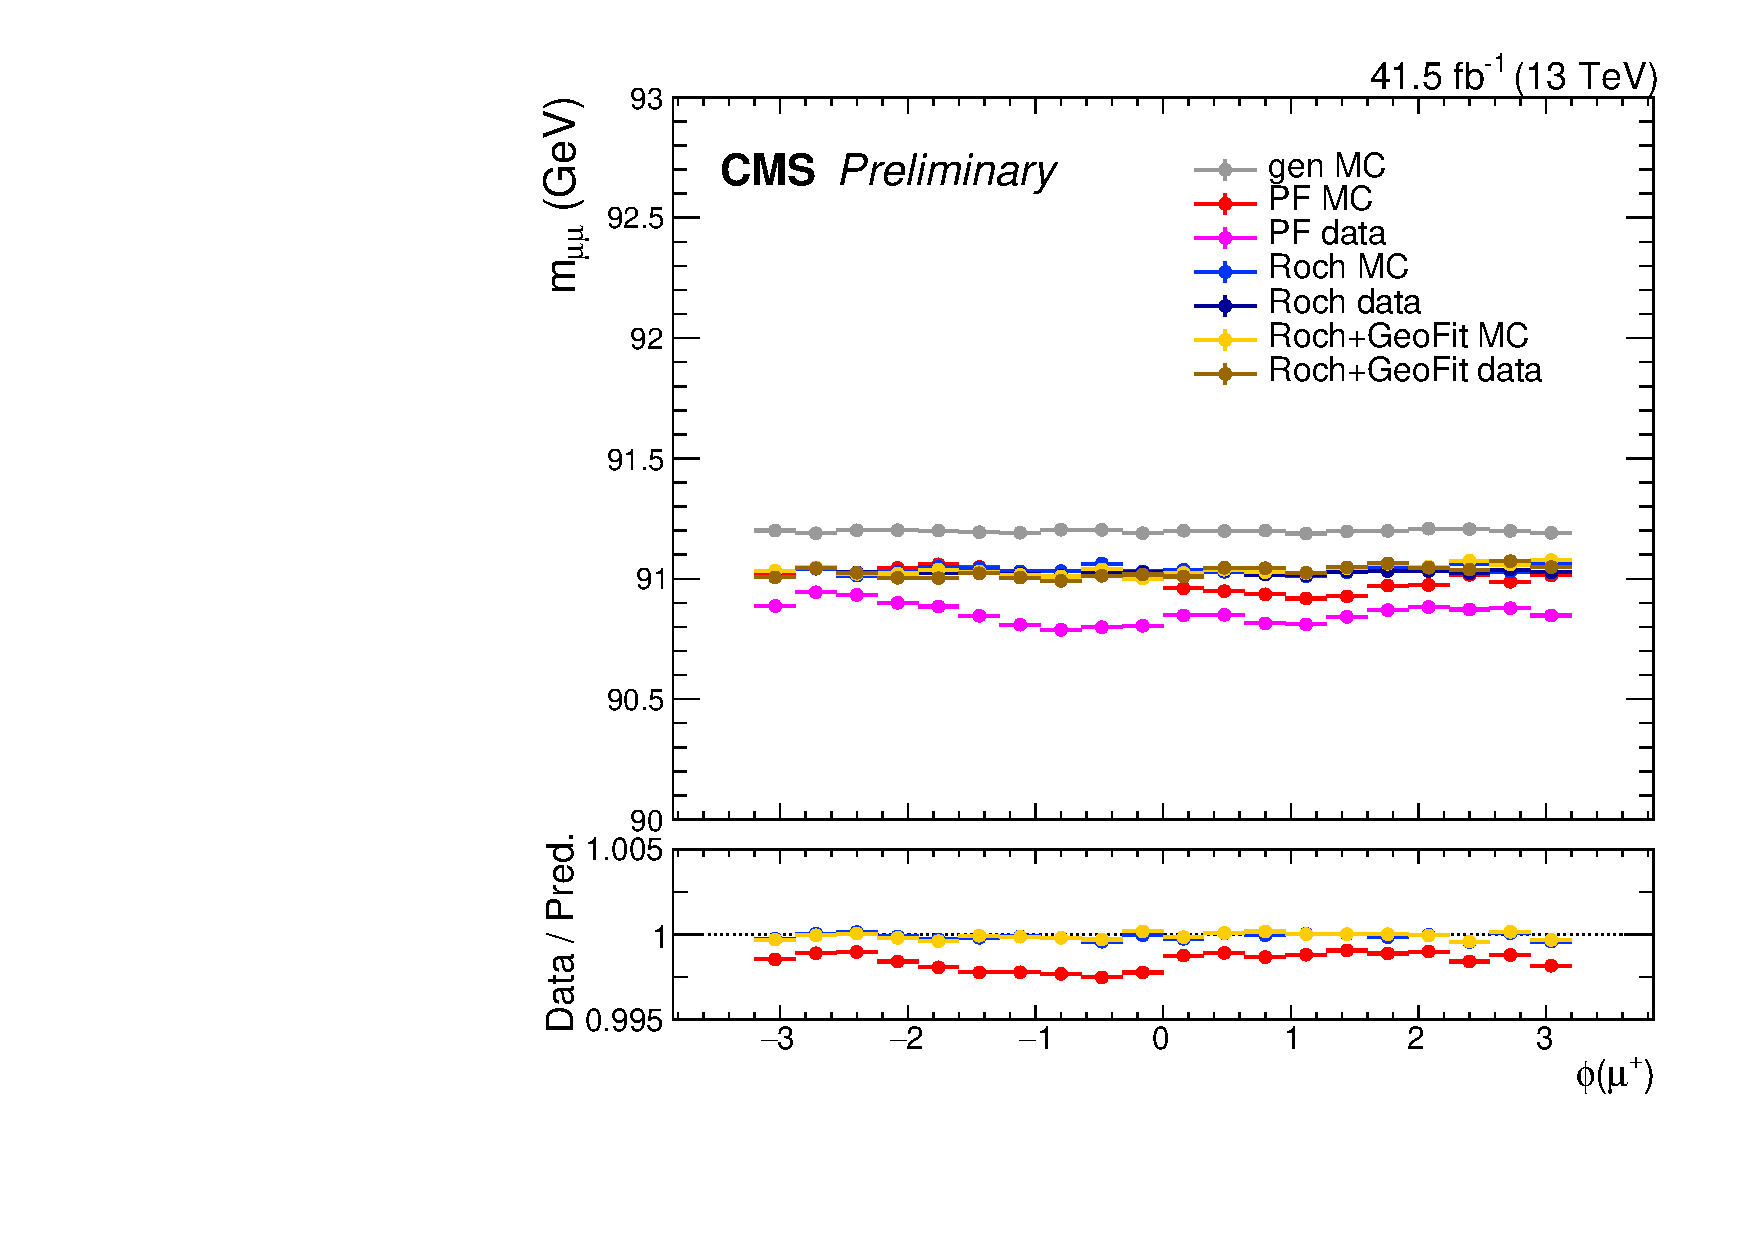
\includegraphics[width=0.32\textwidth]{pics/muon_corr/muon_cal/2017/muP_phi_summary_mean.pdf}
      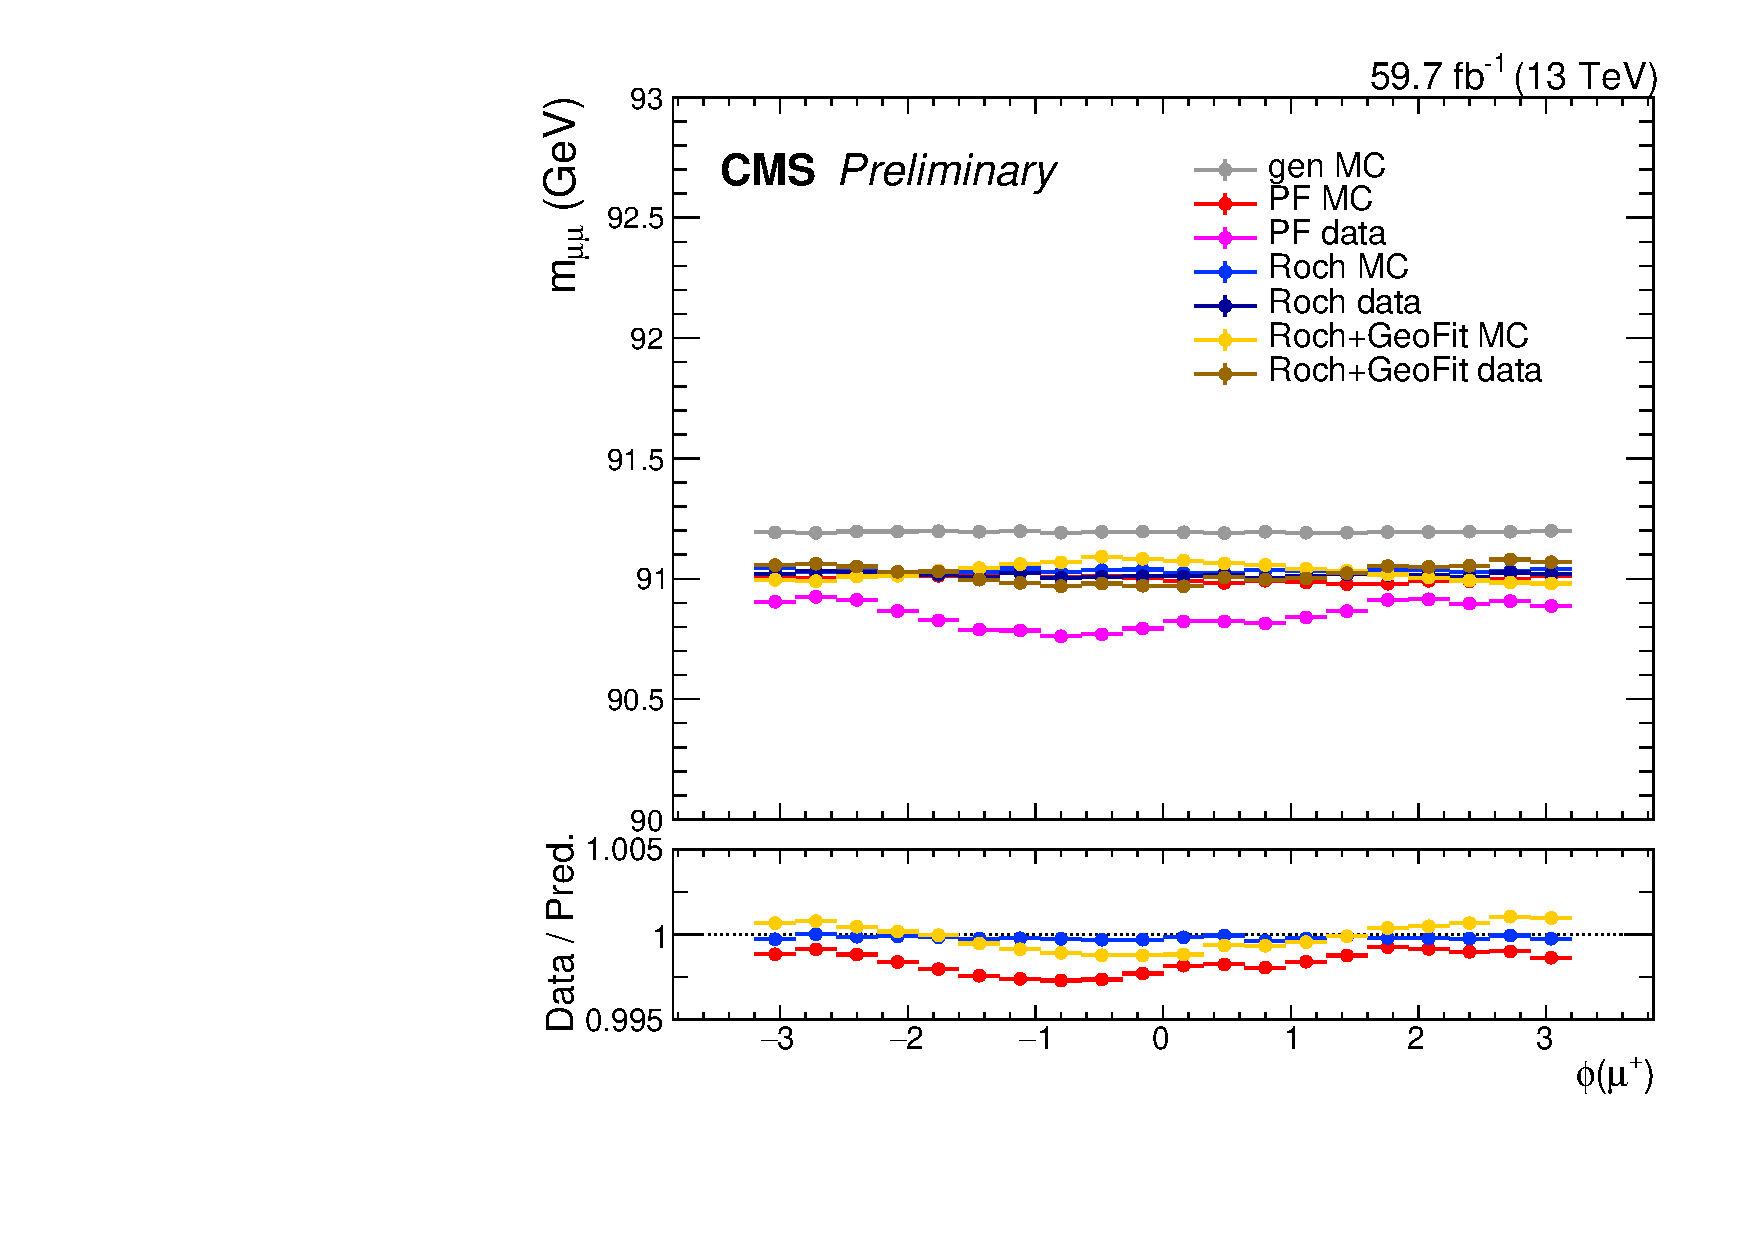
\includegraphics[width=0.32\textwidth]{pics/muon_corr/muon_cal/2018/muP_phi_summary_mean.pdf}
      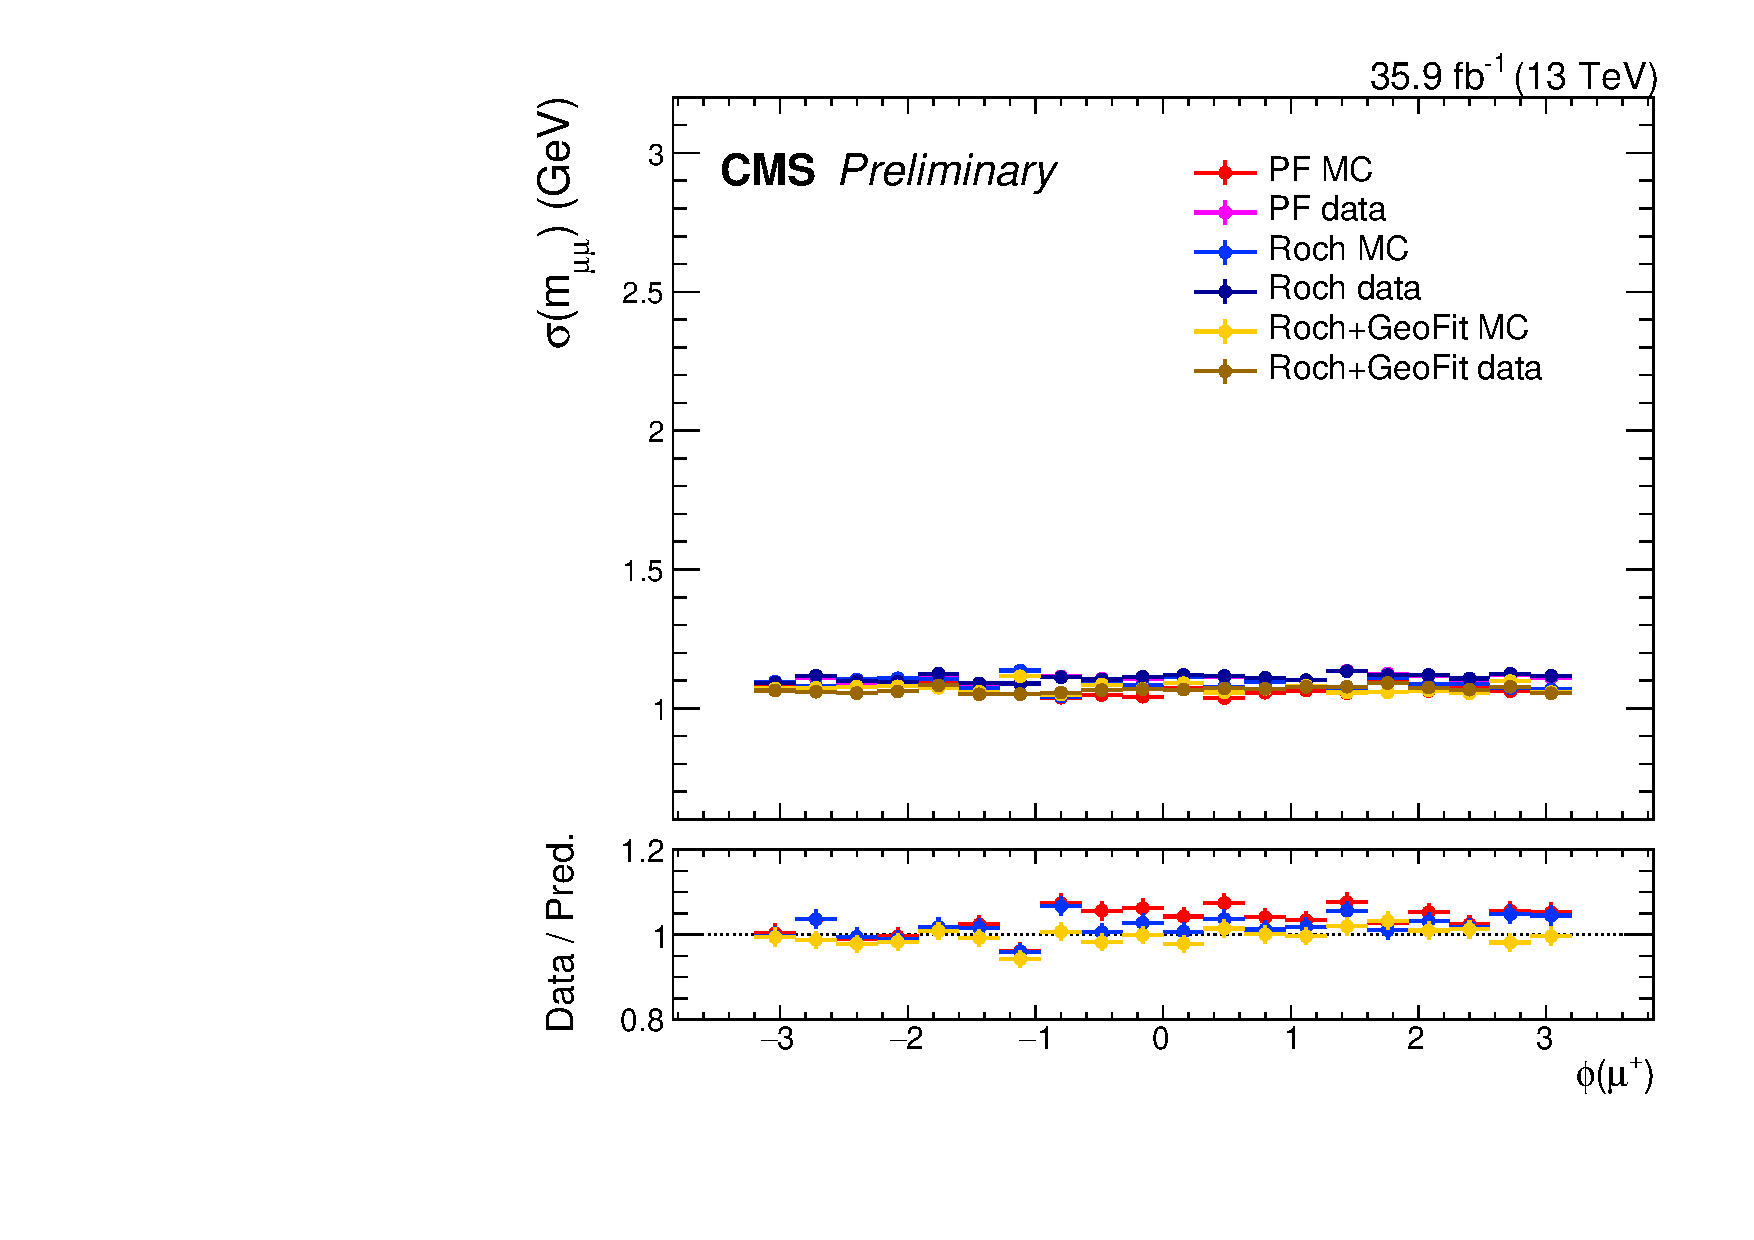
\includegraphics[width=0.32\textwidth]{pics/muon_corr/muon_cal/2016/muP_phi_summary_reso.pdf}
      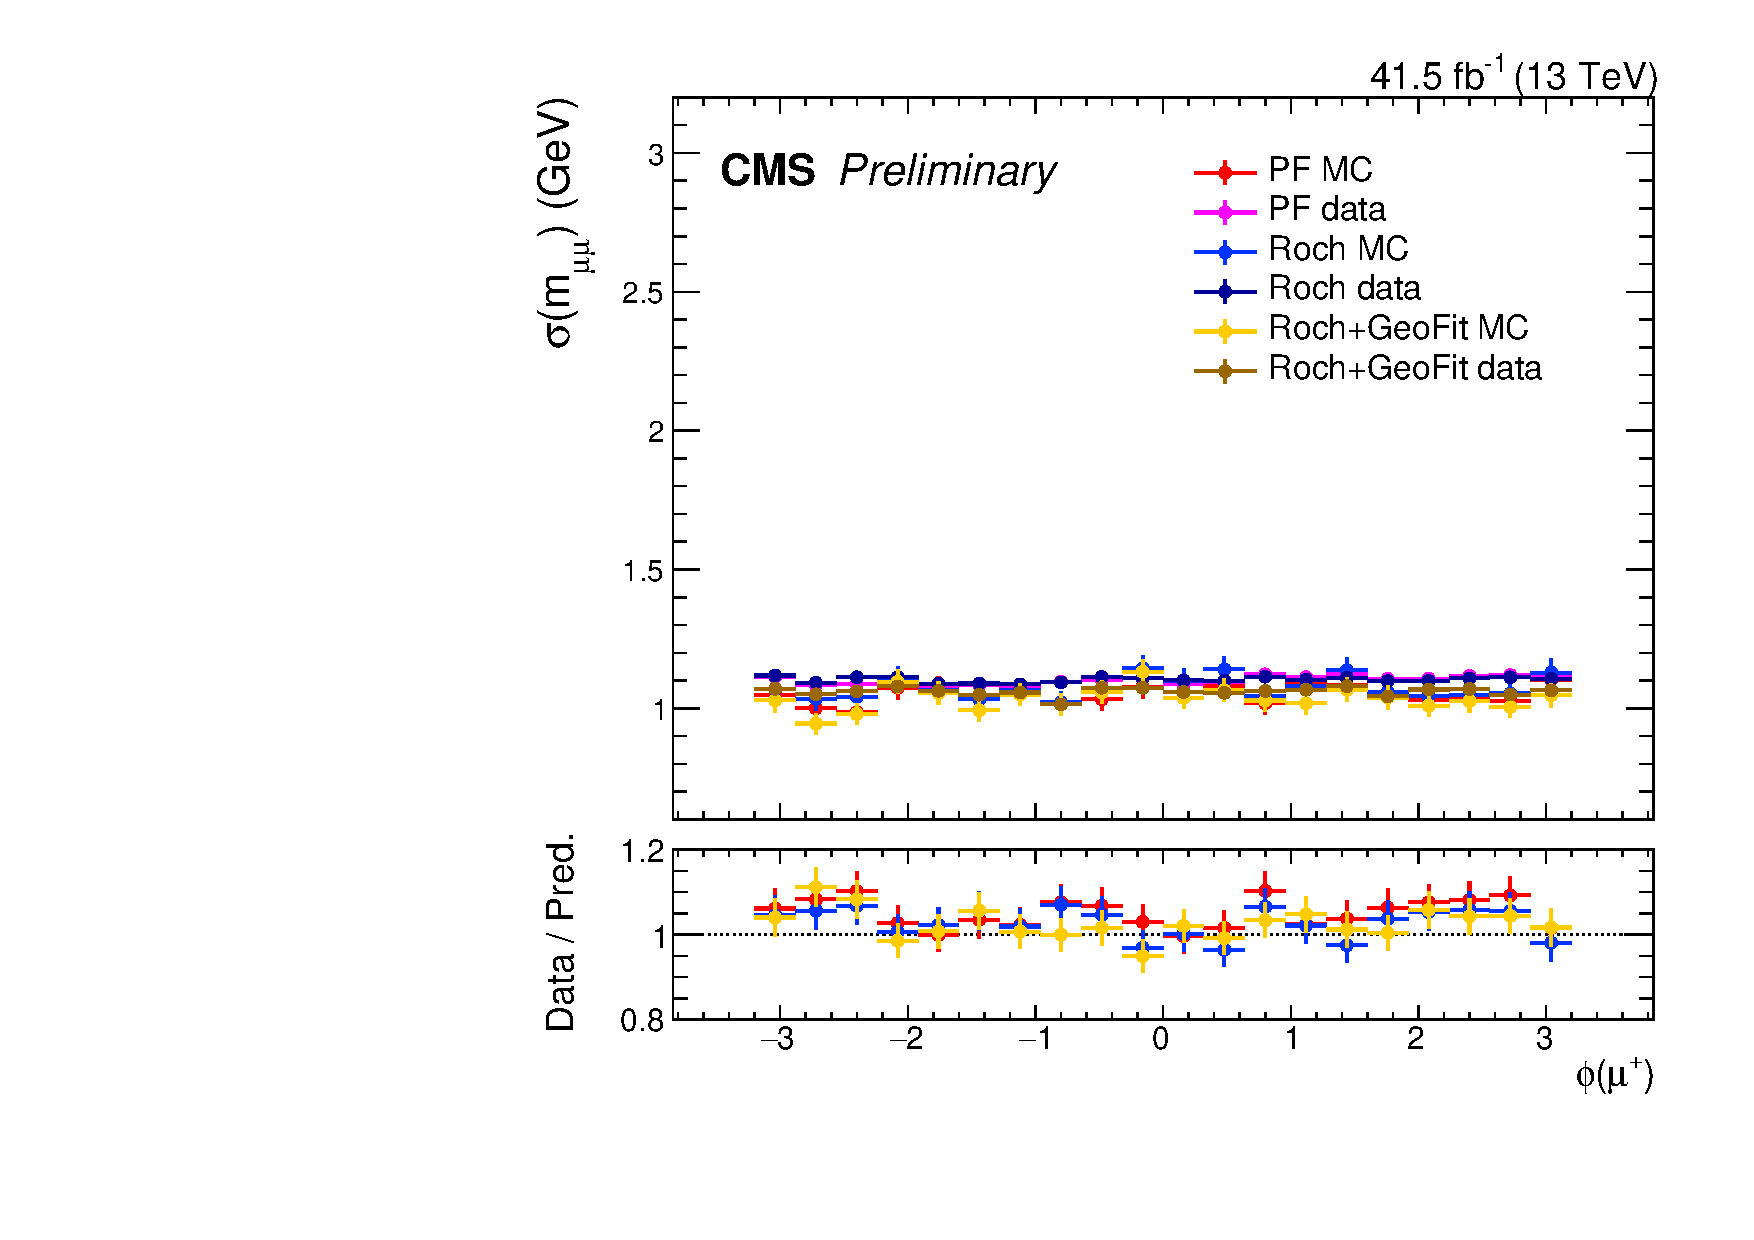
\includegraphics[width=0.32\textwidth]{pics/muon_corr/muon_cal/2017/muP_phi_summary_reso.pdf}
      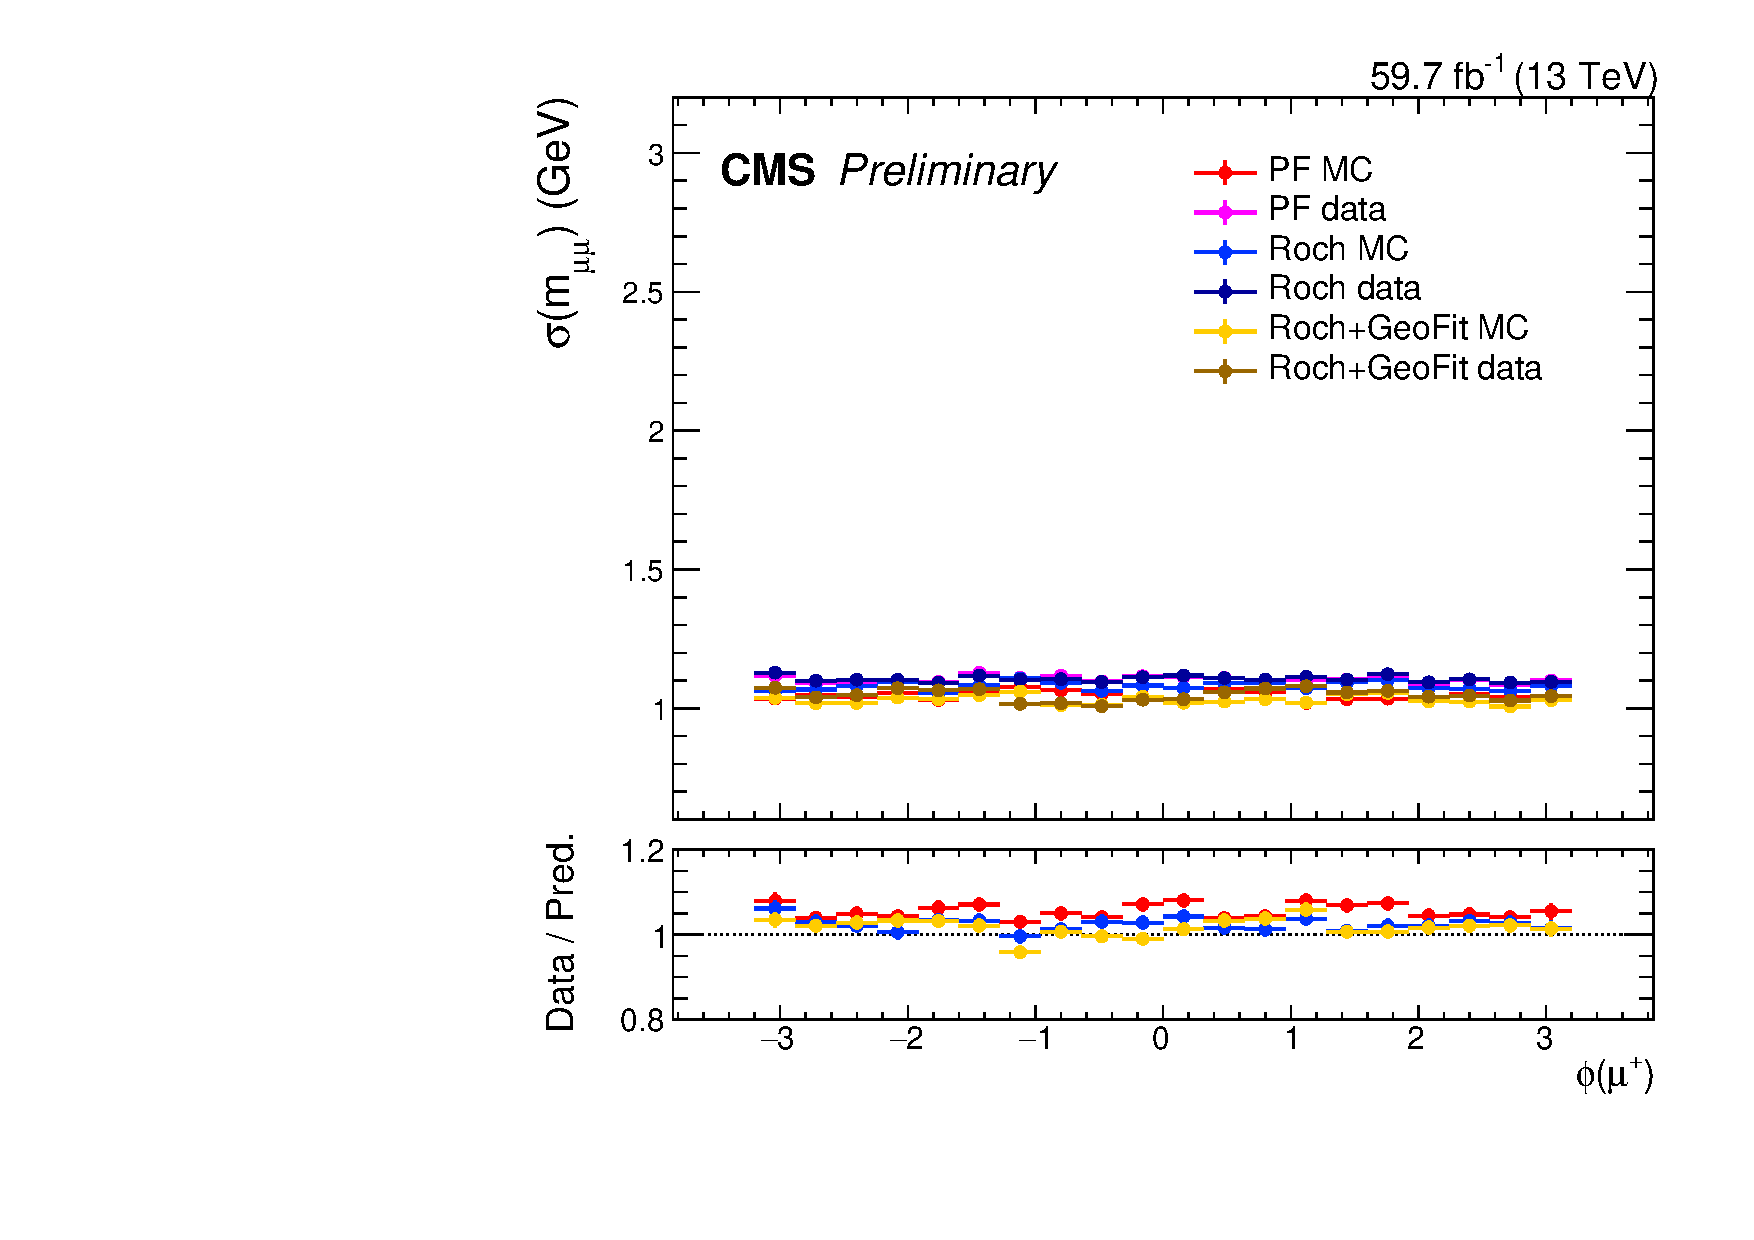
\includegraphics[width=0.32\textwidth]{pics/muon_corr/muon_cal/2018/muP_phi_summary_reso.pdf}
      \caption{Muon calibration plots vs $\phi(\mu^{+})$, for 2016 (left column), 2017 (middle column) and 2018 (right column).
              The top row shows the mean value of the Voigtian fit to the \mmm distribution, 
              while the bottom row shows its experimental resolution.}
      \label{fig:mucal_muP_phi}
\end{figure*}


\begin{figure*}[!htb]
      \centering
      \captionsetup{justification=justified}
      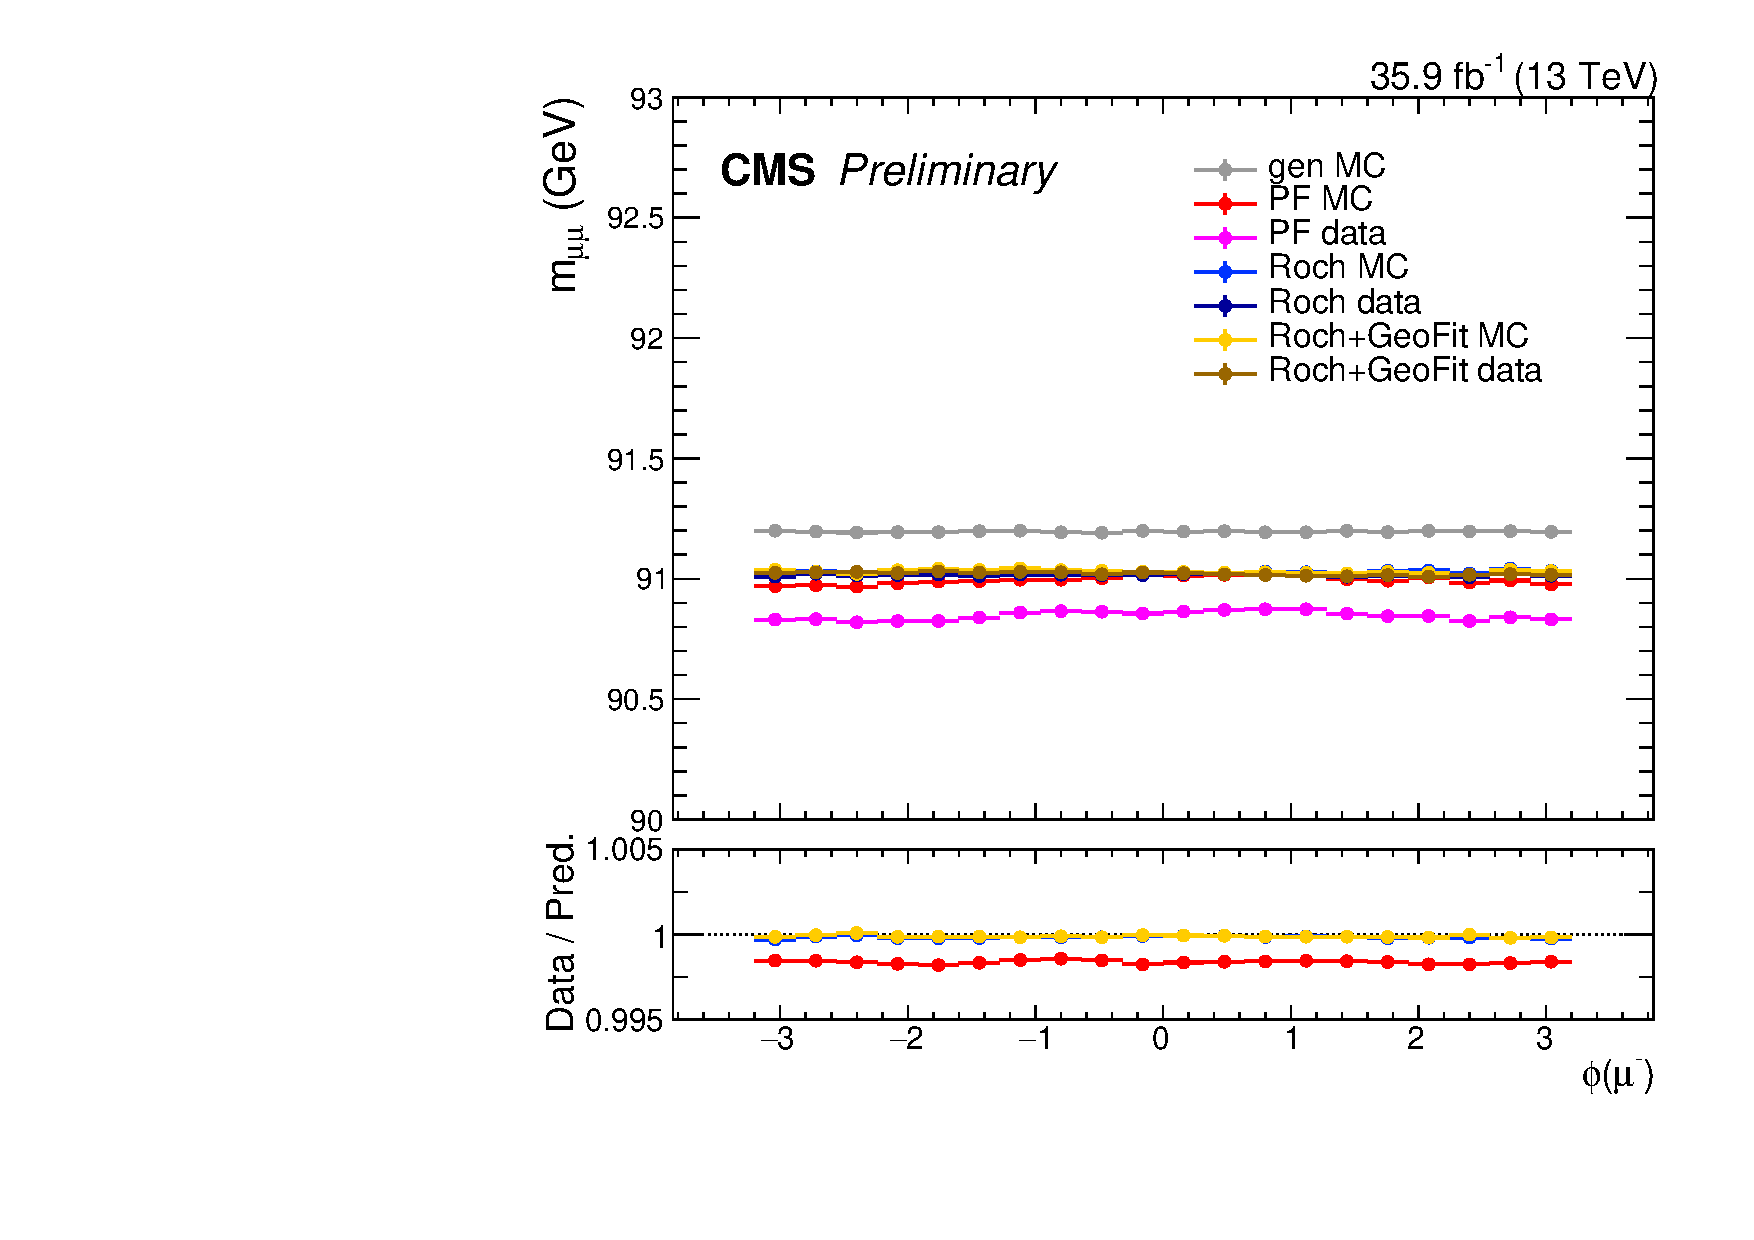
\includegraphics[width=0.32\textwidth]{pics/muon_corr/muon_cal/2016/muN_phi_summary_mean.pdf}
      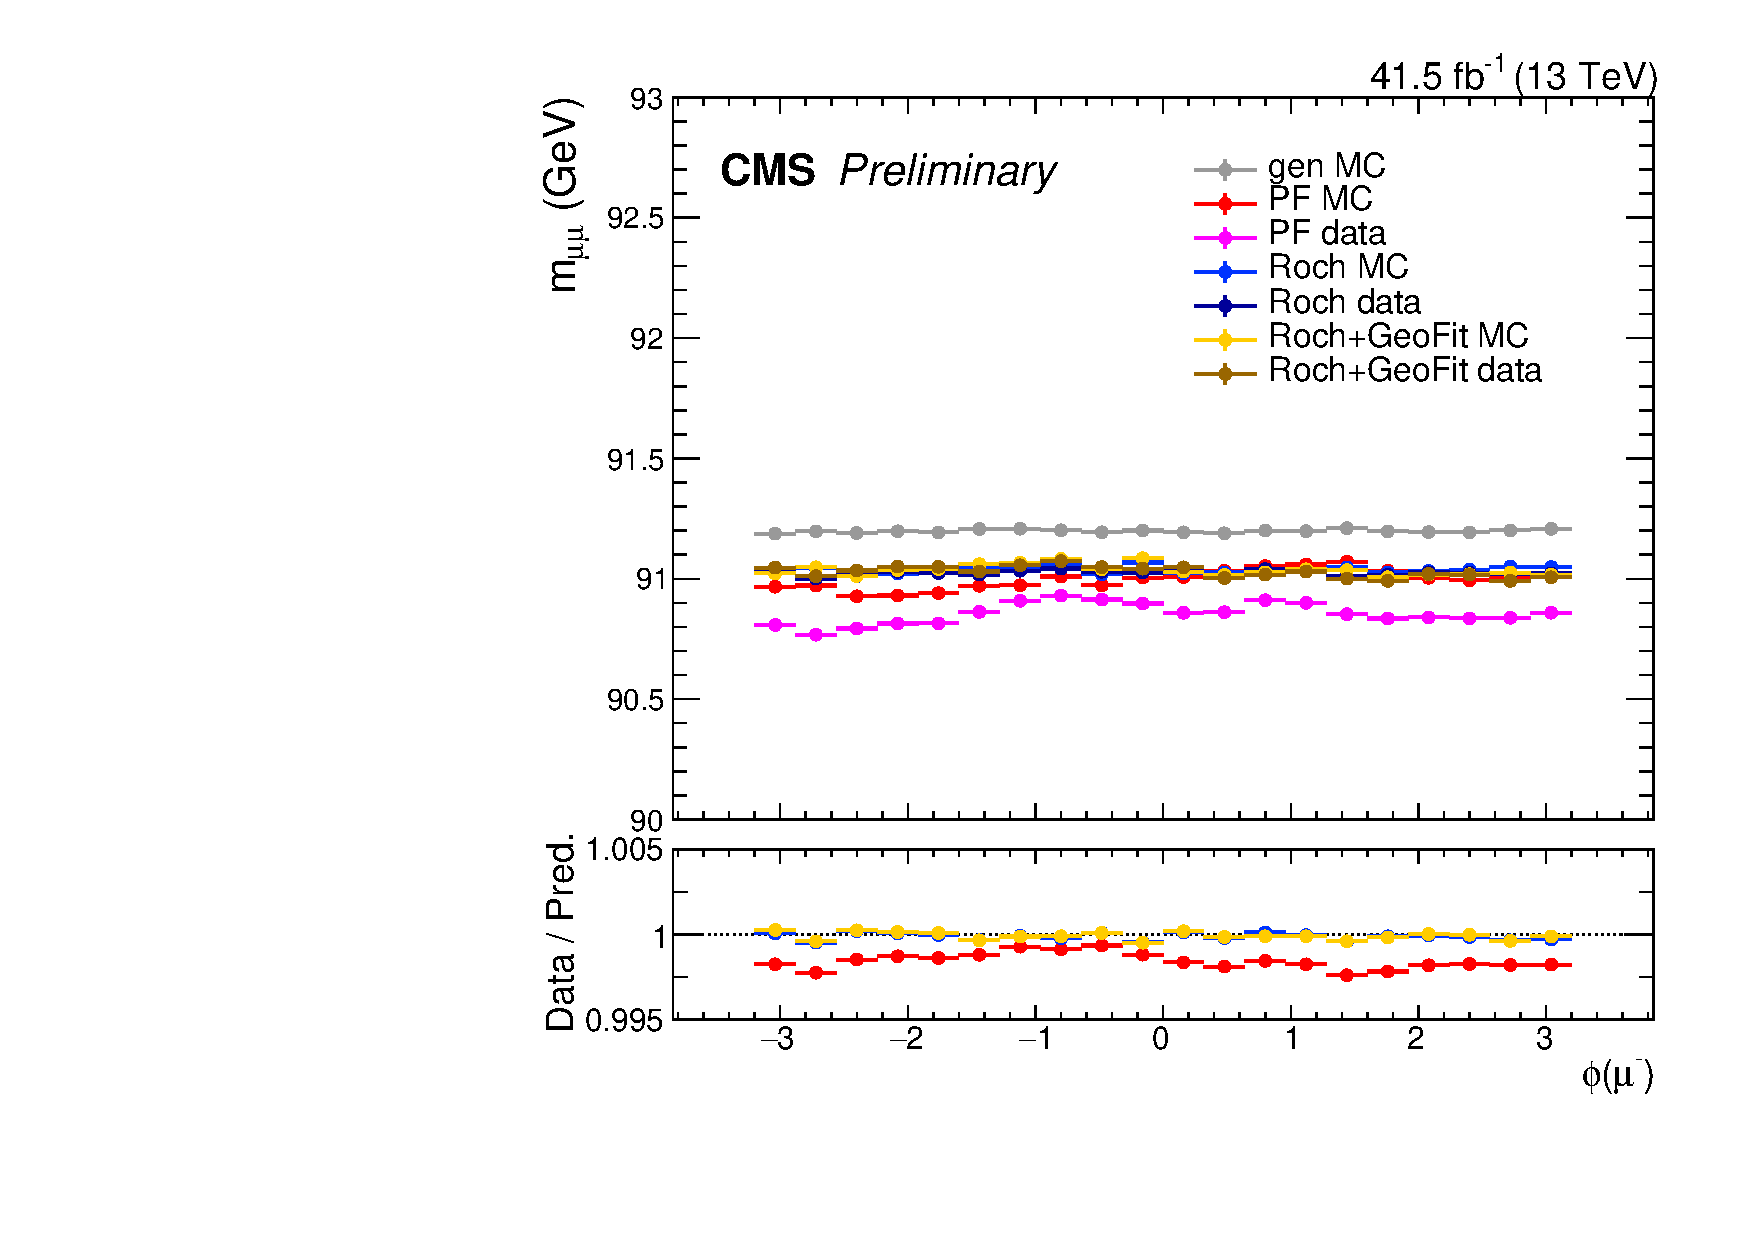
\includegraphics[width=0.32\textwidth]{pics/muon_corr/muon_cal/2017/muN_phi_summary_mean.pdf}
      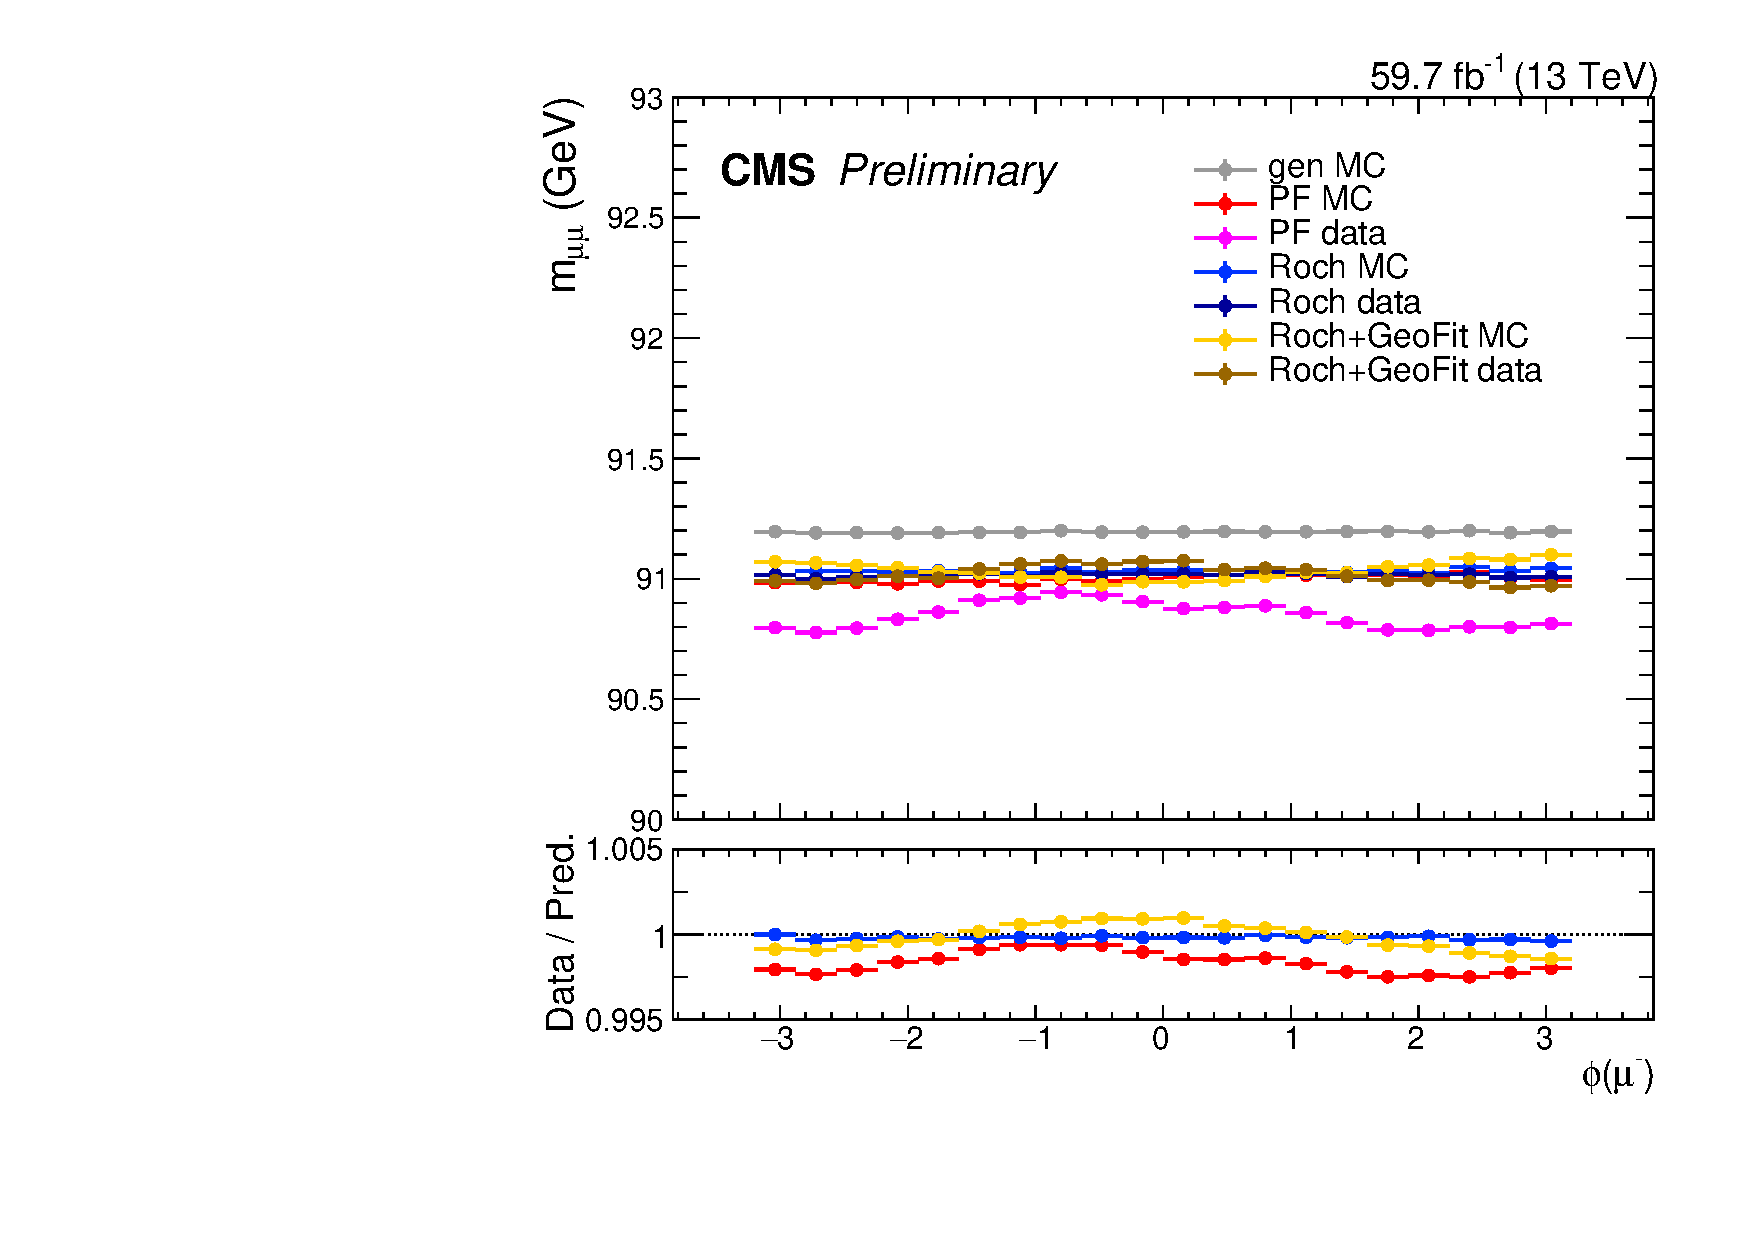
\includegraphics[width=0.32\textwidth]{pics/muon_corr/muon_cal/2018/muN_phi_summary_mean.pdf}
      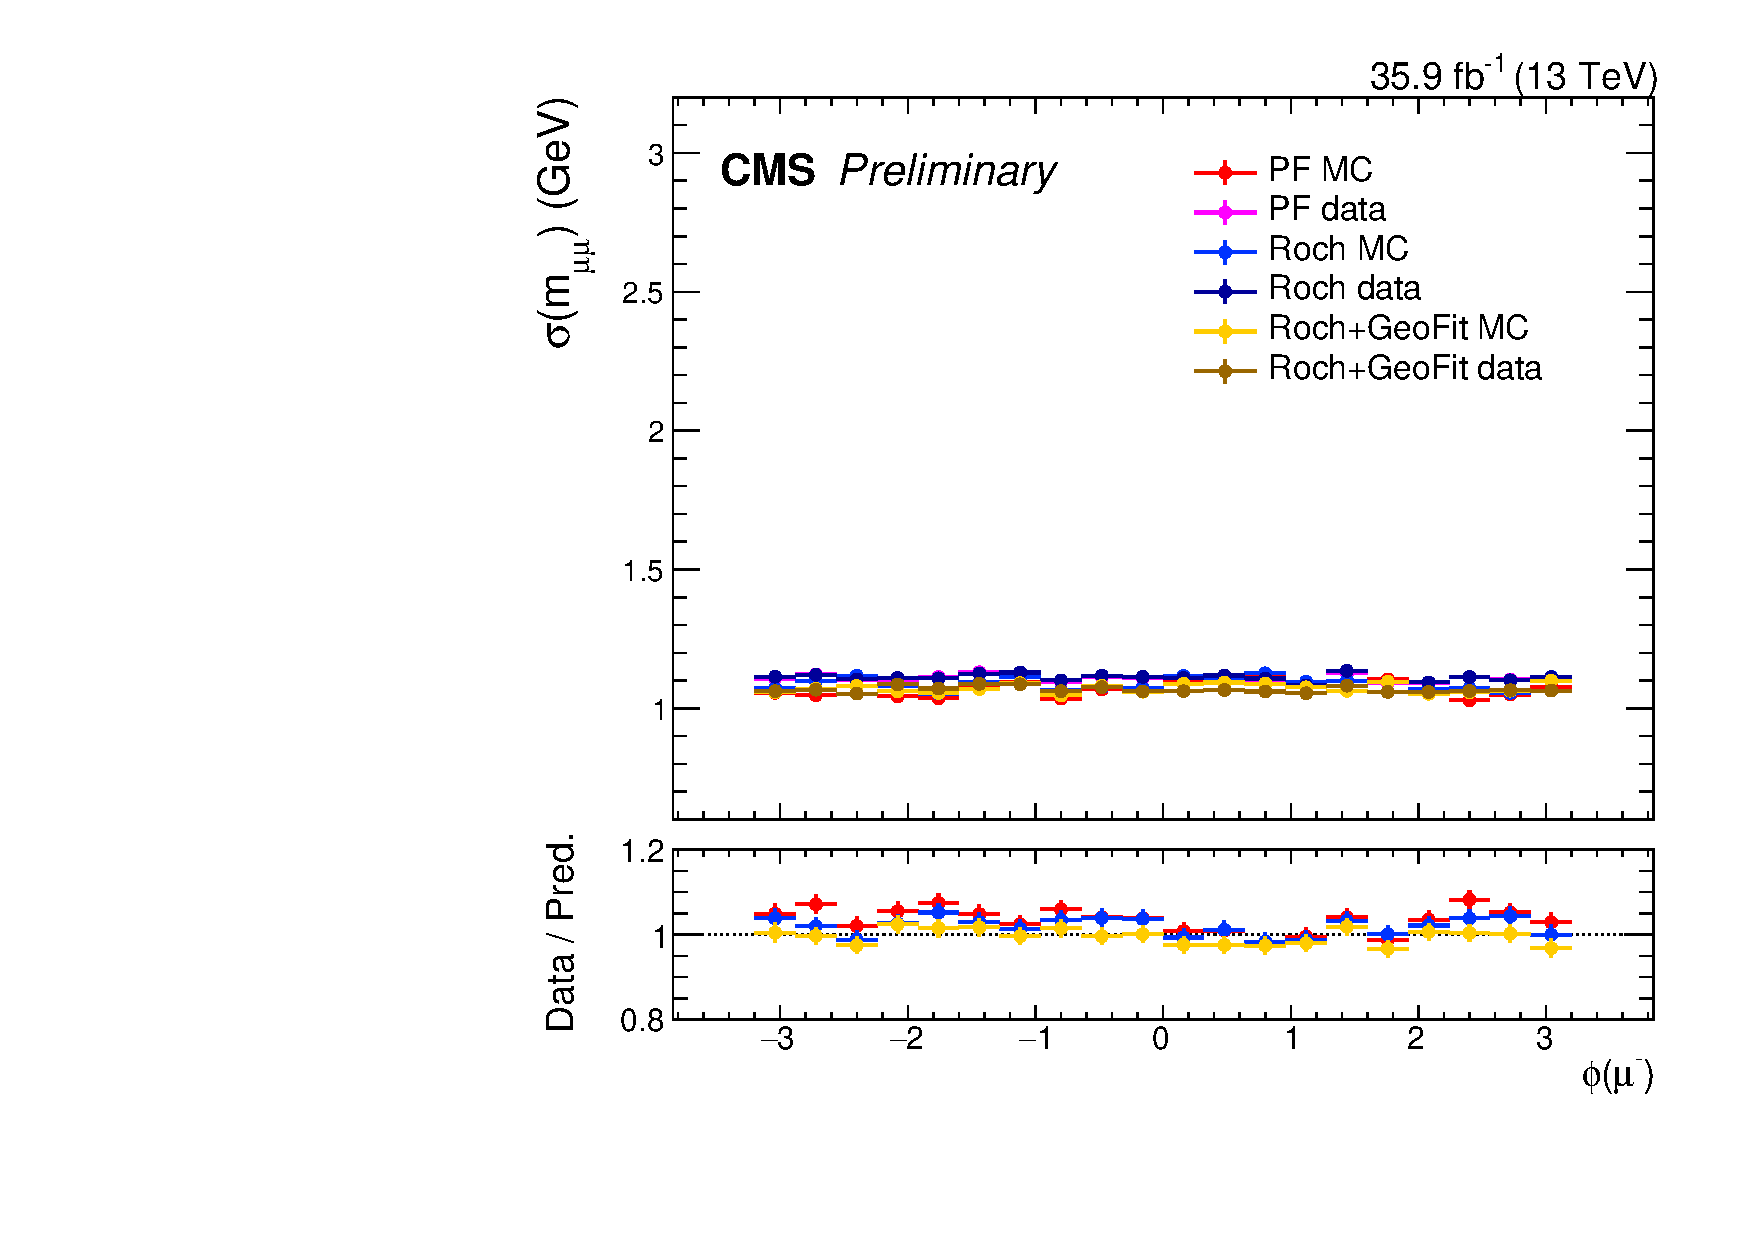
\includegraphics[width=0.32\textwidth]{pics/muon_corr/muon_cal/2016/muN_phi_summary_reso.pdf}
      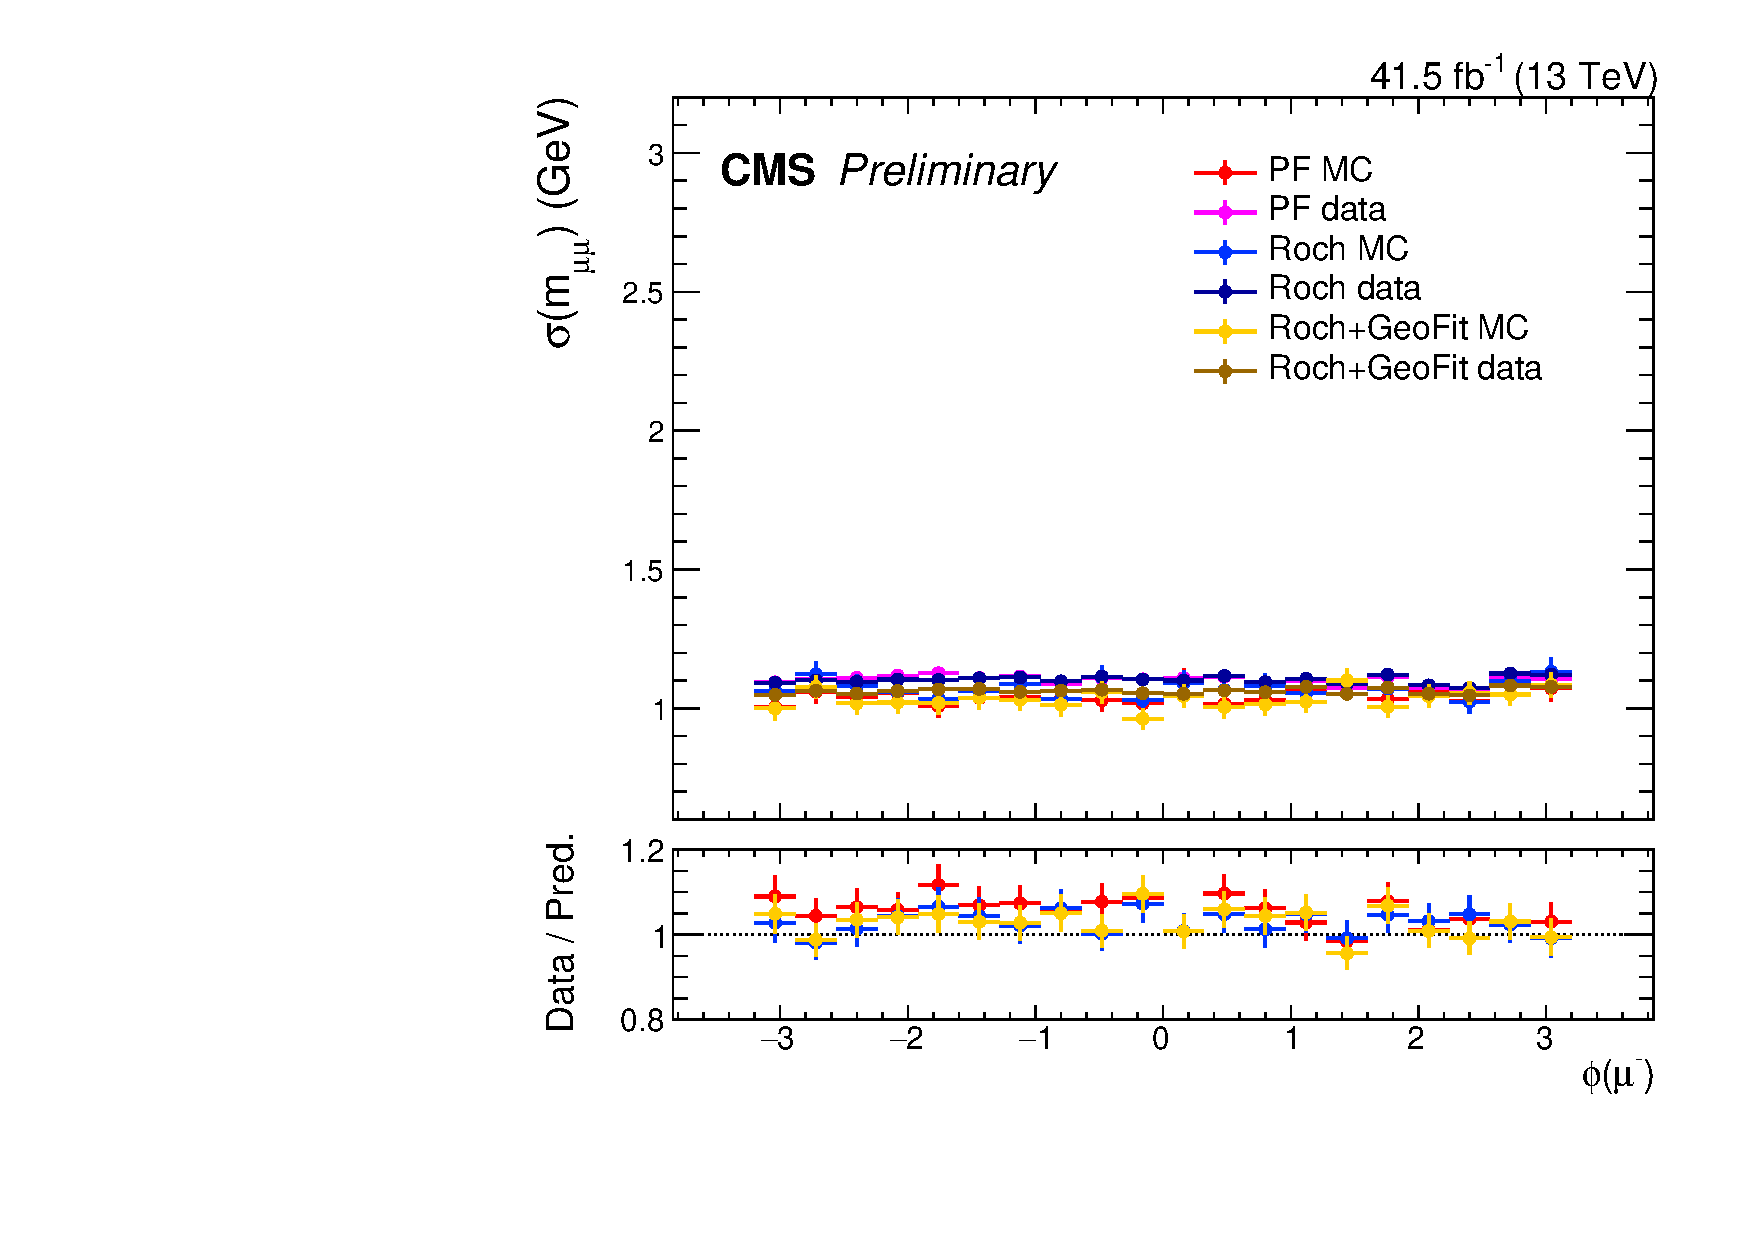
\includegraphics[width=0.32\textwidth]{pics/muon_corr/muon_cal/2017/muN_phi_summary_reso.pdf}
      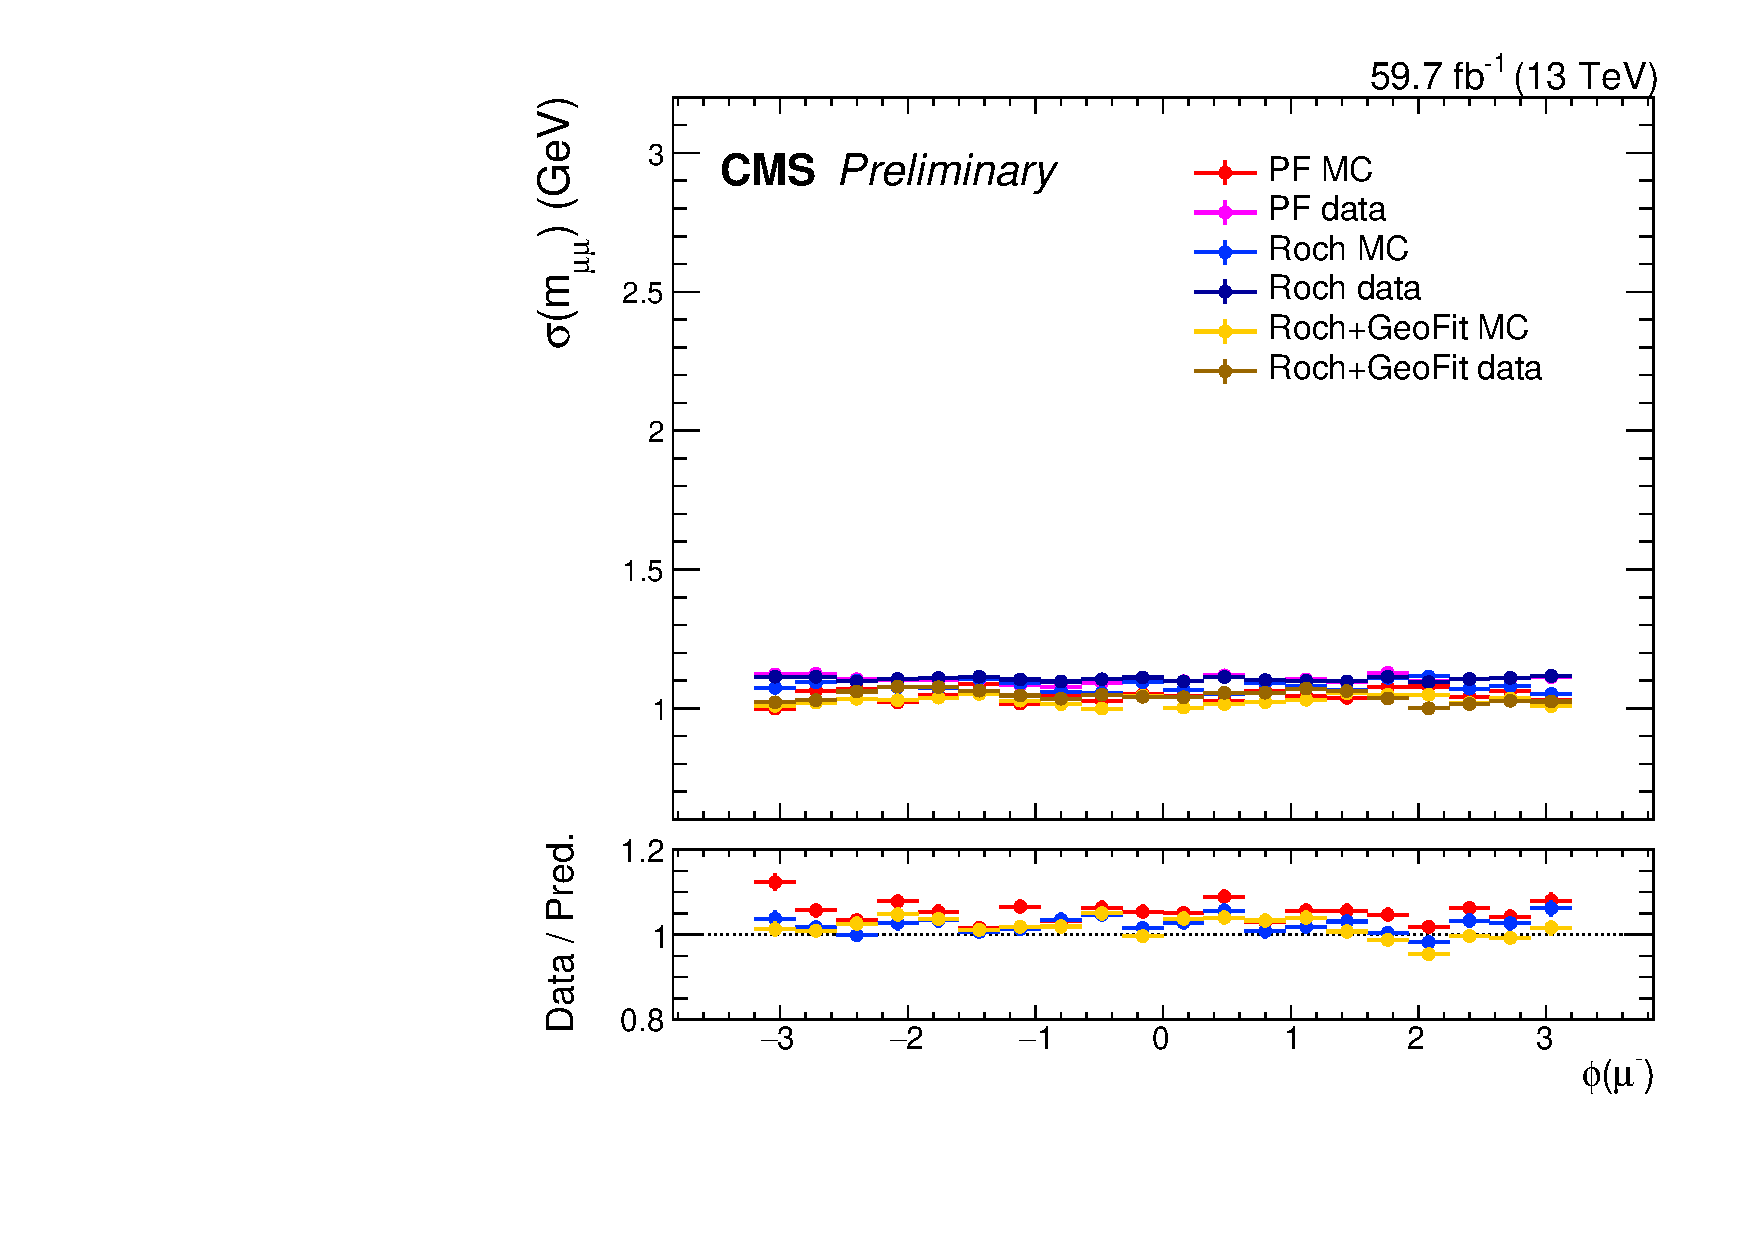
\includegraphics[width=0.32\textwidth]{pics/muon_corr/muon_cal/2018/muN_phi_summary_reso.pdf}
      \caption{Muon calibration plots vs $\phi(\mu^{-})$, for 2016 (left column), 2017 (middle column) and 2018 (right column).
               The top row shows the mean value of the Voigtian fit to the \mmm distribution, 
               while the bottom row shows its experimental resolution.}
      \label{fig:mucal_muN_phi}
\end{figure*}


\begin{figure*}[!htb]
      \centering
      \captionsetup{justification=justified}
      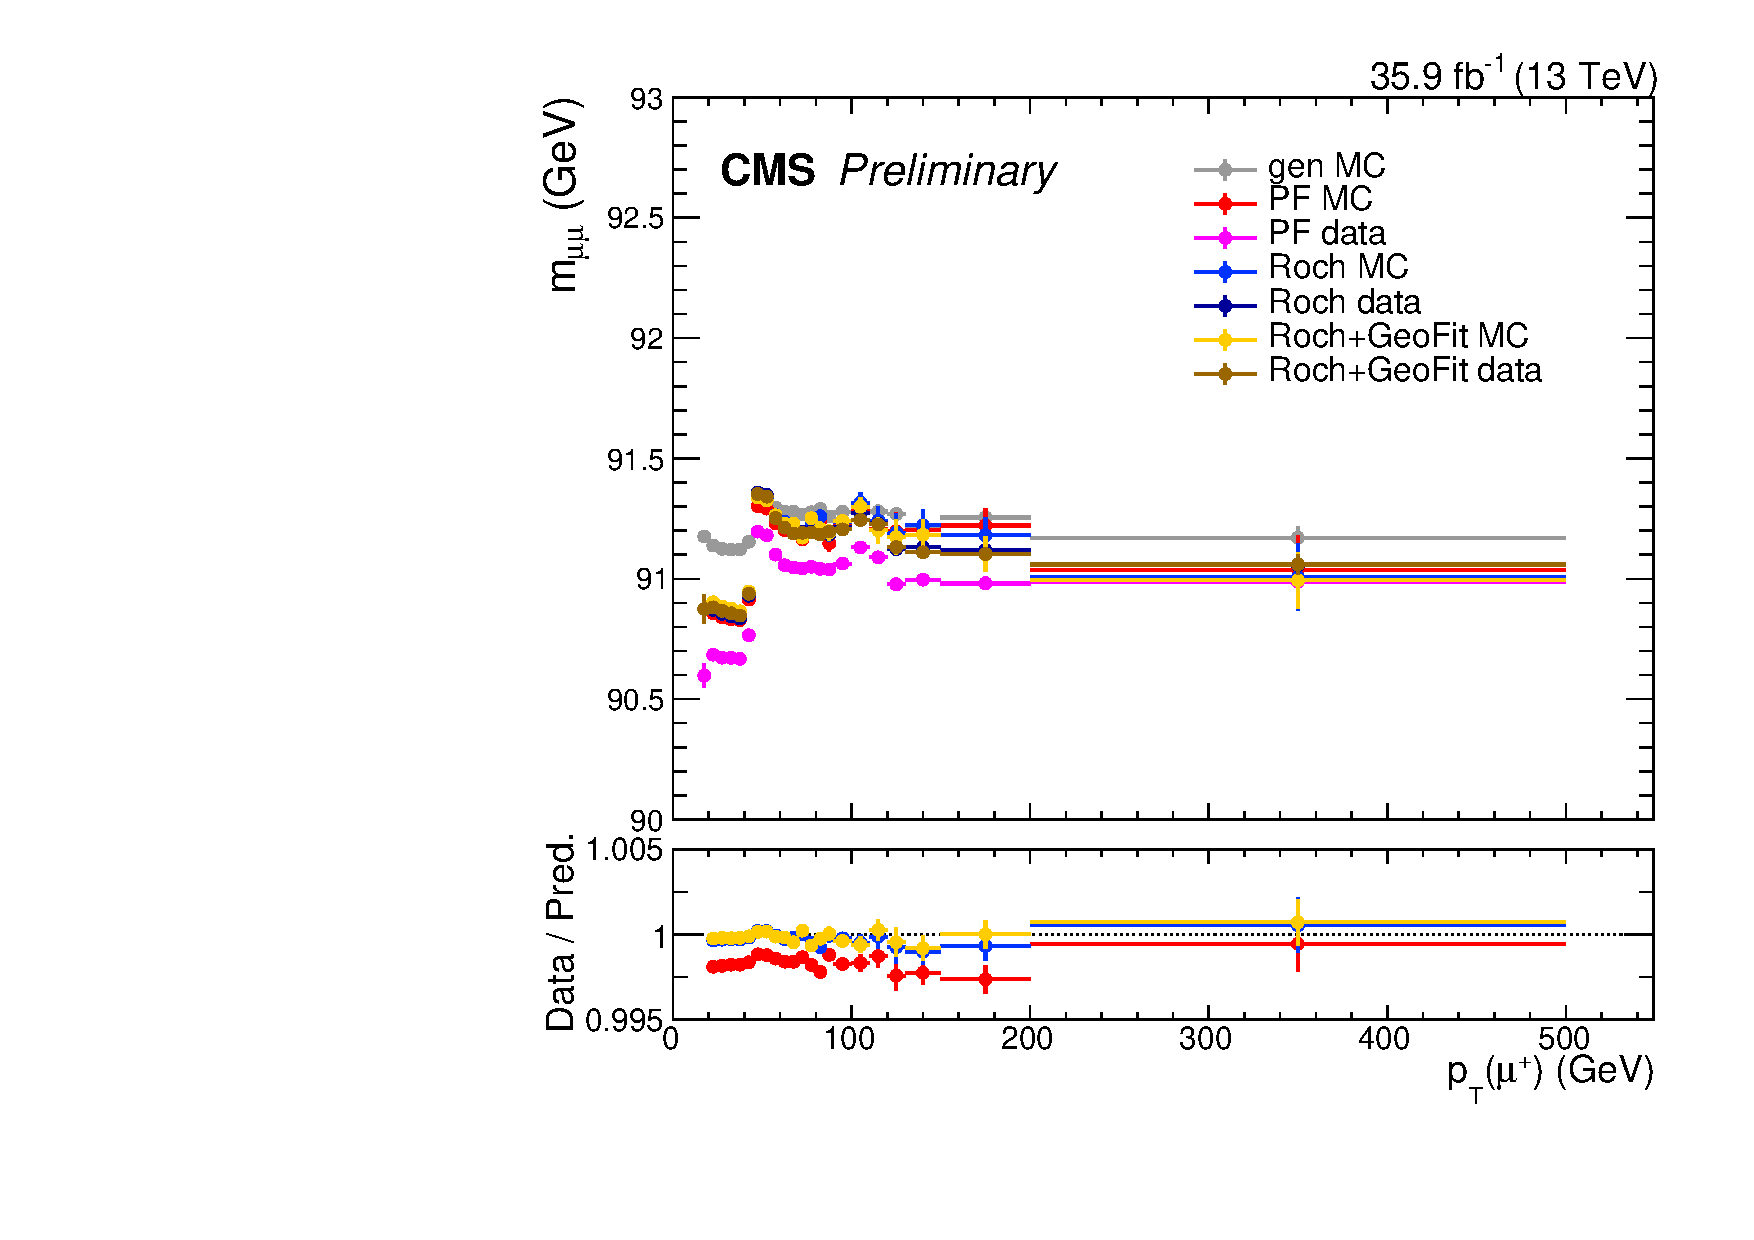
\includegraphics[width=0.32\textwidth]{pics/muon_corr/muon_cal/2016/muP_pt_summary_mean.pdf}
      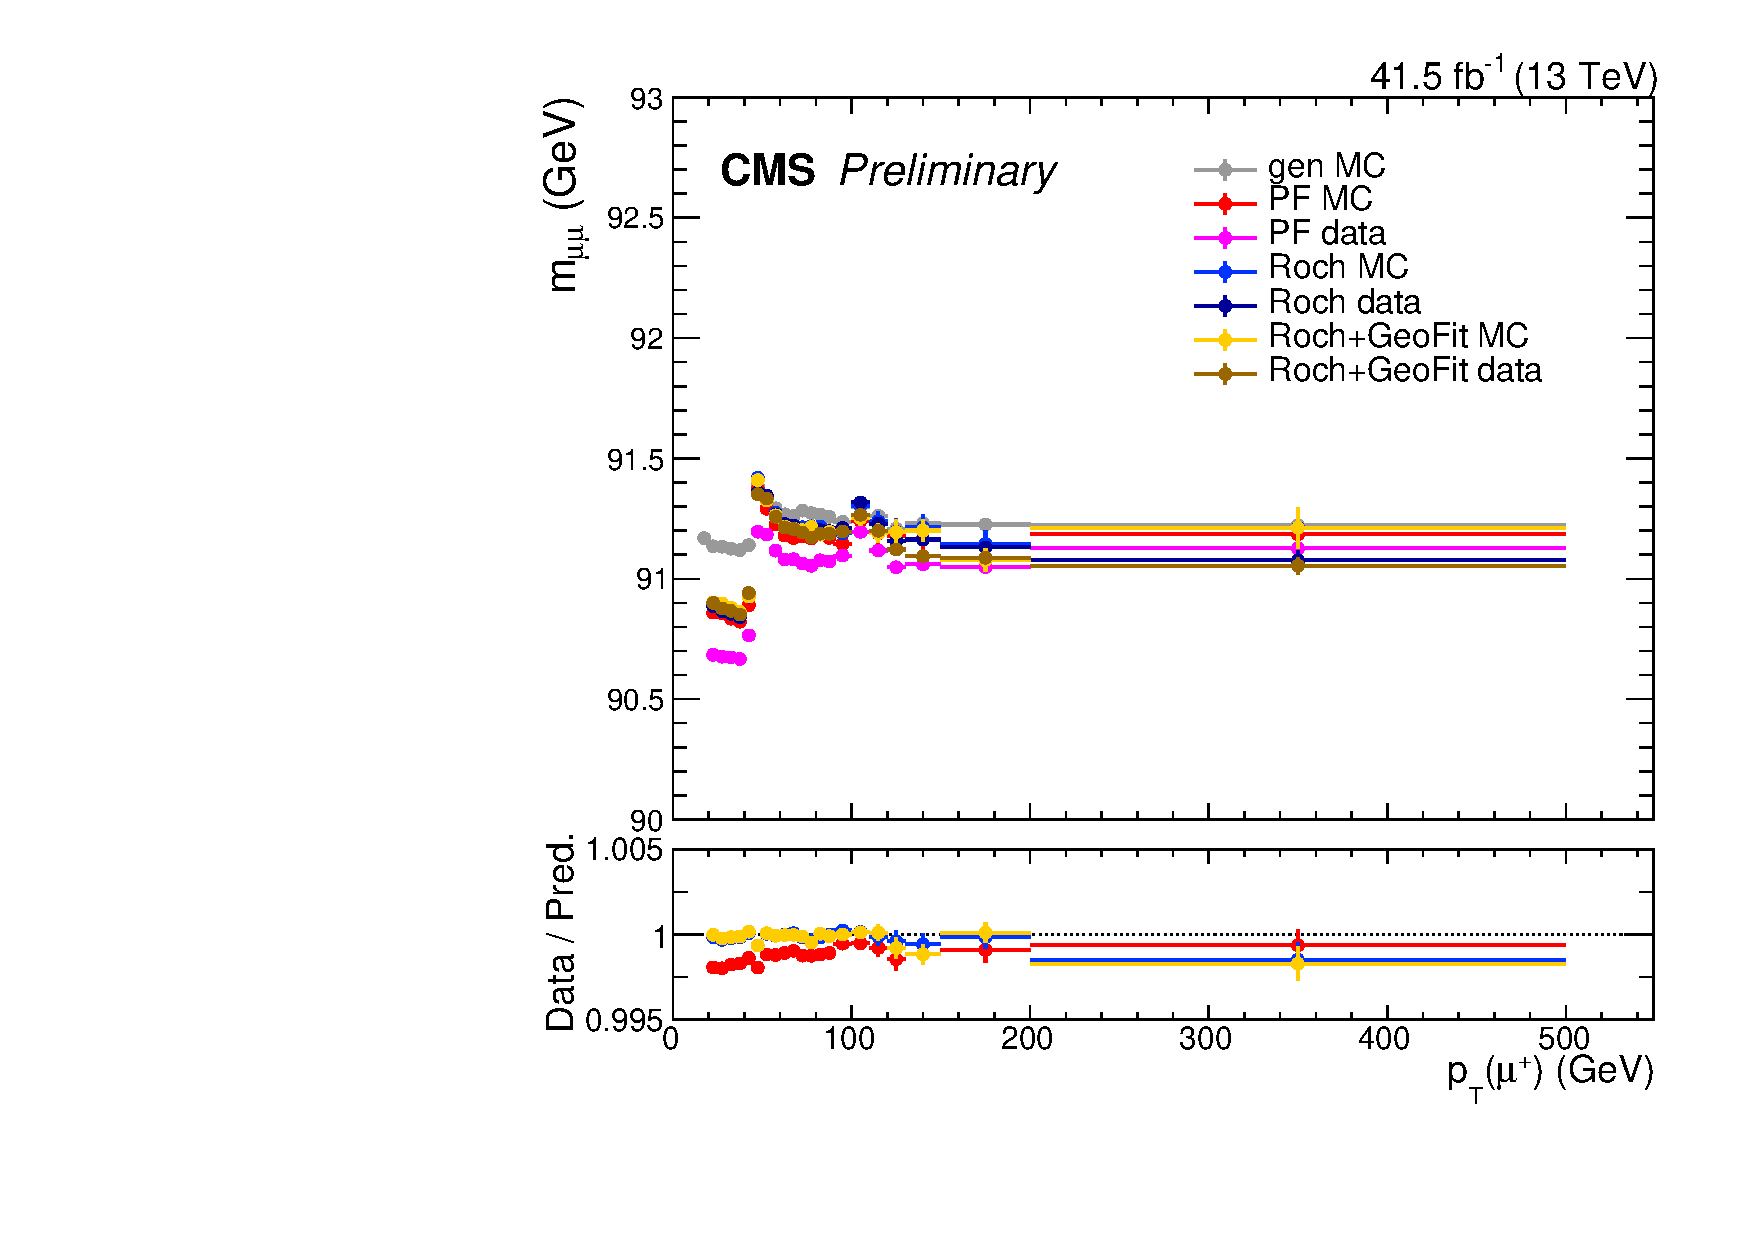
\includegraphics[width=0.32\textwidth]{pics/muon_corr/muon_cal/2017/muP_pt_summary_mean.pdf}
      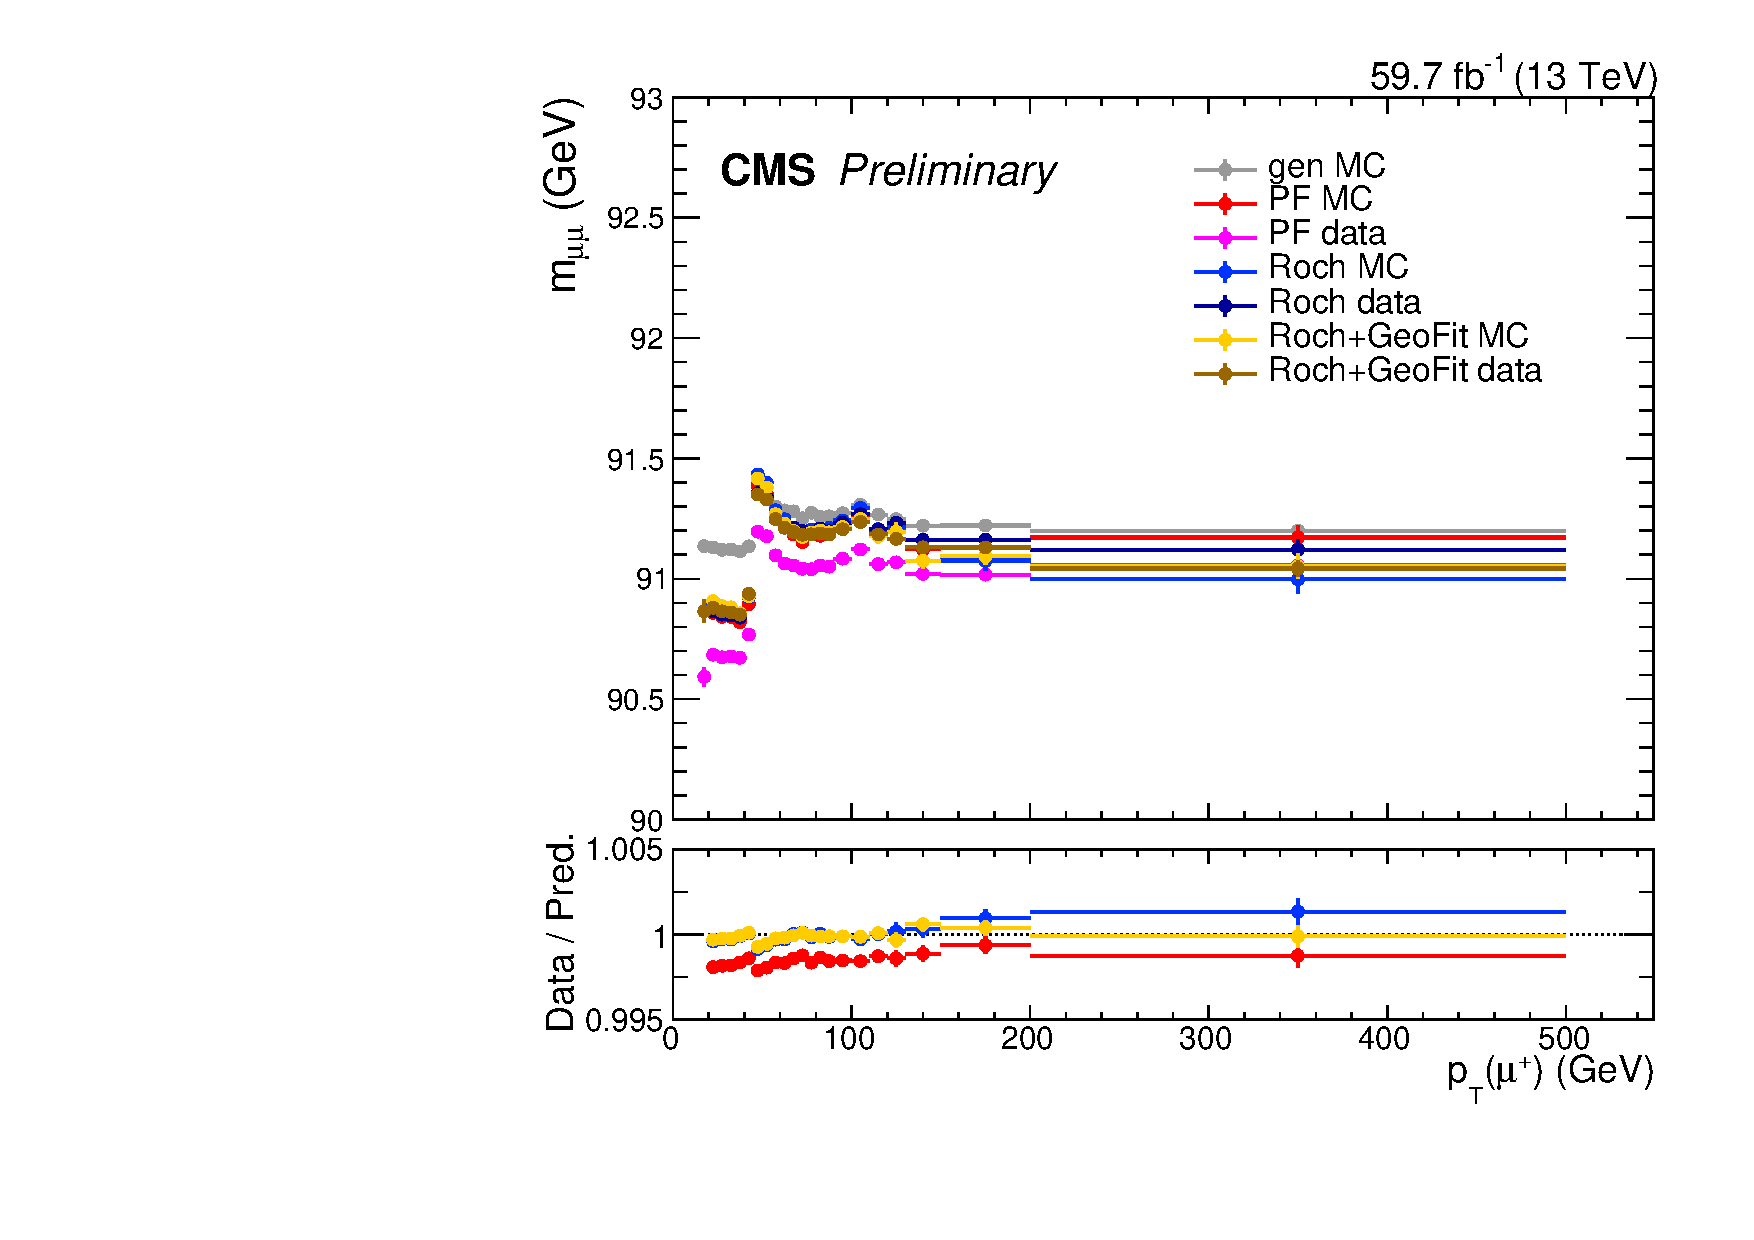
\includegraphics[width=0.32\textwidth]{pics/muon_corr/muon_cal/2018/muP_pt_summary_mean.pdf}
      \includegraphics[width=0.32\textwidth]{pics/muon_corr/muon_cal/2016/muP_pt_summary_reso.pdf}
      \includegraphics[width=0.32\textwidth]{pics/muon_corr/muon_cal/2017/muP_pt_summary_reso.pdf}
      \includegraphics[width=0.32\textwidth]{pics/muon_corr/muon_cal/2018/muP_pt_summary_reso.pdf}
      \caption{Muon calibration plots vs $\pt(\mu^{+})$, for 2016 (left column), 2017 (middle column) and 2018 (right column).
               The top row shows the mean value of the Voigtian fit to the \mmm distribution, 
               while the bottom row shows its experimental resolution.
               The \pt binning sculpts the shape of the \mmm peak, which leads to a jump at the \pt = 45 \GeV in the plots.}
      \label{fig:mucal_muP_pt}
\end{figure*}


\begin{figure*}[!htb]
      \centering
      \captionsetup{justification=justified}
      \includegraphics[width=0.32\textwidth]{pics/muon_corr/muon_cal/2016/dimu_pt_summary_mean.pdf}
      \includegraphics[width=0.32\textwidth]{pics/muon_corr/muon_cal/2017/dimu_pt_summary_mean.pdf}
      \includegraphics[width=0.32\textwidth]{pics/muon_corr/muon_cal/2018/dimu_pt_summary_mean.pdf}
      \includegraphics[width=0.32\textwidth]{pics/muon_corr/muon_cal/2016/dimu_pt_summary_reso.pdf}
      \includegraphics[width=0.32\textwidth]{pics/muon_corr/muon_cal/2017/dimu_pt_summary_reso.pdf}
      \includegraphics[width=0.32\textwidth]{pics/muon_corr/muon_cal/2018/dimu_pt_summary_reso.pdf}
      \caption{Muon calibration plots vs $\pt(\mu\mu)$, for 2016 (left column), 2017 (middle column) and 2018 (right column).
               The top row shows the mean value of the Voigtian fit to the \mmm distribution, 
               while the bottom row shows its experimental resolution.}
      \label{fig:mucal_dimu_pt}
\end{figure*}


\begin{figure*}[!htb]
      \centering
      \captionsetup{justification=justified}
      \includegraphics[width=0.32\textwidth]{pics/muon_corr/muon_cal/2016/dimu_eta_summary_mean.pdf}
      \includegraphics[width=0.32\textwidth]{pics/muon_corr/muon_cal/2017/dimu_eta_summary_mean.pdf}
      \includegraphics[width=0.32\textwidth]{pics/muon_corr/muon_cal/2018/dimu_eta_summary_mean.pdf}
      \includegraphics[width=0.32\textwidth]{pics/muon_corr/muon_cal/2016/dimu_eta_summary_reso.pdf}
      \includegraphics[width=0.32\textwidth]{pics/muon_corr/muon_cal/2017/dimu_eta_summary_reso.pdf}
      \includegraphics[width=0.32\textwidth]{pics/muon_corr/muon_cal/2018/dimu_eta_summary_reso.pdf}
      \caption{Muon calibration plots vs $\eta(\mu\mu)$, for 2016 (left column), 2017 (middle column) and 2018 (right column).
               The top row shows the mean value of the Voigtian fit to the \mmm distribution, 
               while the bottom row shows its experimental resolution.}
      \label{fig:mucal_dimu_eta}
\end{figure*}


\begin{figure*}[!htb]
      \centering
      \captionsetup{justification=justified}
      \includegraphics[width=0.32\textwidth]{pics/muon_corr/muon_cal/2016/muP_d0_rebin_summary_mean.pdf}
      \includegraphics[width=0.32\textwidth]{pics/muon_corr/muon_cal/2017/muP_d0_rebin_summary_mean.pdf}
      \includegraphics[width=0.32\textwidth]{pics/muon_corr/muon_cal/2018/muP_d0_rebin_summary_mean.pdf}
      \includegraphics[width=0.32\textwidth]{pics/muon_corr/muon_cal/2016/muP_d0_rebin_summary_reso.pdf}
      \includegraphics[width=0.32\textwidth]{pics/muon_corr/muon_cal/2017/muP_d0_rebin_summary_reso.pdf}
      \includegraphics[width=0.32\textwidth]{pics/muon_corr/muon_cal/2018/muP_d0_rebin_summary_reso.pdf}
      \caption{Muon calibration plots vs $d_0(\mu^{+})$, for 2016 (left column), 2017 (middle column) and 2018 (right column).
               The top row shows the mean value of the Voigtian fit to the \mmm distribution, 
               while the bottom row shows its experimental resolution.}
      \label{fig:mucal_muP_d0}
\end{figure*}


\begin{figure*}[!htb]
      \centering
      \captionsetup{justification=justified}
      \includegraphics[width=0.32\textwidth]{pics/muon_corr/muon_cal/2016/muN_d0_rebin_summary_mean.pdf}
      \includegraphics[width=0.32\textwidth]{pics/muon_corr/muon_cal/2017/muN_d0_rebin_summary_mean.pdf}
      \includegraphics[width=0.32\textwidth]{pics/muon_corr/muon_cal/2018/muN_d0_rebin_summary_mean.pdf}
      \includegraphics[width=0.32\textwidth]{pics/muon_corr/muon_cal/2016/muN_d0_rebin_summary_reso.pdf}
      \includegraphics[width=0.32\textwidth]{pics/muon_corr/muon_cal/2017/muN_d0_rebin_summary_reso.pdf}
      \includegraphics[width=0.32\textwidth]{pics/muon_corr/muon_cal/2018/muN_d0_rebin_summary_reso.pdf}
      \caption{Muon calibration plots vs $d_0(\mu^{-})$, for 2016 (left column), 2017 (middle column) and 2018 (right column).
               The top row shows the mean value of the Voigtian fit to the \mmm distribution, 
               while the bottom row shows its experimental resolution.}
      \label{fig:mucal_muN_d0}
\end{figure*}
\chapter{Search for H2Mu targeting the VH production mode}

As described in Section~\ref{sec:hmm_cat_and_strategy}, the analysis in the \VH category targets the \VH production modes of the Higgs boson, 
and is established as two independent parts, the \WH category and the \ZH category.
This chapter provides a full description of the procedures and the results in these two categories.
In this chapter the \VH category will sometimes be referred to as the \VH categories, 
when we focus more on the individual specifications of the \WH and \ZH categories, rather than their common characteristics.

The \VH analyses focus on the leptonic ($e$ or $\mu$) decay modes of the \PV boson (\PW or \PZ), 
which leads to distinct final states involving extra well-reconstructed charged lepton(s) in addition to the two muons from the Higgs decay.
By requiring these additional leptons, the main backgrounds in the generic $\mu\mu$ phase-space, the \DY and the \ttbar processes, are greatly suppressed,
leading to a high \SoB in the \VH categories, and ensuring a good expected significance with only a handful of signal events.
The other decay modes of the \PV boson are disregarded for different reasons:

The \PV bosons decay to tau leptons ($\PW \to \tau+\PGn_{\tau}$, or $\PZ \to \tau\bar{\tau}$) at the same rate as they decay to electrons or muons. 
However, in CMS, the reconstruction of $\tau$ is not as efficient as that of electrons or muons: 
the reconstruction of the hadronic decays of $\tau$ suffers from a sizable fake rate, 
while the leptonic decays of $\tau$ would just appear as an electron or a muon of much lower \pt.
Tagging the hadronic decays of taus from the \PW or \PZ decay would lead to a much lower \SoB than the $e$ and $\mu$ tags in the current \VH analyses,
bringing negligible contribution to the overall sensitivity.
As for the leptonic decays of $\tau$, they are not explicitly vetoed.
If any \VH signal events containing such decays pass the selection, they are considered as part of the signal contribution.
Although, this contribution is small, as the $e$ or $\mu$ from the $\tau$ decay would most likely fail the \pt or the vertex proximity cuts.

The hadronic decays of the \PW or the \PZ boson lead to two jets in the event, making an invariant mass near the mean mass of the boson.
Although amounting to a larger branching ratio than the leptonic decay modes, these hadronic decays turned out not as helpful in enriching the \VH events.
A selection based on the dijet invariant mass could pick most of the \VH events, but in the meantime collect a much larger amount of $\ggH+$jets and \qqH events, 
as well as an immense background of $\DY+$jets and \ttbar processes.
The \SoB from this selection is not very high, as this phase-space is dominated by $\ggH+$jets vs $\DY+$jets events.
Up to the time of this report, no kinematic handle is found to be particularly effective in enriching the hadronic \VH signal.
Therefore, the hadronic \VH events are considered as minor signal contributions in the \ggH category, 
and no dedicated \VH hadronic tag is deployed.

The \PZ boson can decay to a pair of neutrinos at a branching ratio of 20\%, 
which leave no electronic signal in the CMS detector and appear as a missing transverse momentum (\MET) in the event.
This \MET equals to the \pt of the \PZ boson and can provide discrimination against some backgrounds.
However, due to the complex hadronic activity in pp collisions and the large uncertainty in the hadronic calorimetry in CMS, 
almost all events are reconstructed with some nonzero \MET, even for events without any real \MET, like the \DY events.
As a result, the purity of the $\ZH \to \nu\nu+\mu\mu$ signal can only be enhanced if a very tight cut on the \MET is applied.
The signal efficiency for this cut is, unfortunately, low, because only a small fraction of the \PZ bosons in \ZH events have high \pt.
Furthermore, after this cut, some large irreducible backgrounds still remain, like the \ttbar and diboson processes.
Overall, a tag for the $\ZH \to \nu\nu+\mu\mu$ would be much less sensitive than the existing $\ZH \to \ell\ell+\mu\mu$ tag, and is not deployed.
The $\ZH \to \nu\nu+\mu\mu$ signal events are considered as minor signal contributions in the \ggH category.

After requiring additional lepton(s) in the event, the main background in the resulting \VH phase-spaces becomes the \WZ and \ZZ processes, for the \WH and \ZH categories respectively.
For both \WZ and \ZZ backgrounds, if more than two muons are present in the event, 
there are different possibilities of the association between the muons and their parent particles.
In fact, the wrong pairing of muons, called the combinatorial background, yields the majority of the \WZ and \ZZ background.
For example, in an on-shell \WZ event, the muon from the \PW decay can be falsely paired with the oppositely signed (OS) muon from the \PZ decay, 
making an invariant mass near the Higgs mass value.
A set of cut-based event selection is optimized to reduced the combinatorial background, further improving the \SoB. 
More details are given in Section~\ref{sec:vh_event_selection}.

The minor backgrounds may include the triboson processes, the \DY process accompanied with additional non-prompt leptons, 
or the \Pqt quark associated processes, for example the \ttbar, $\Pqt\PW$, and $\ttbar\PV$ processes, 
where the \Pqb quarks from the top decays either fall out of the acceptance of the detector or fails the b-tagging. 
All these minor backgrounds have different kinematic profiles from the signal and can be reduced to different extents. 
Boosted Decision Tree (BDT) discriminators are trained in both the \WH and the \ZH categories to account for the differences between the signal and the inclusive background as much as possible.

With the BDT discriminators, events are further divided in to several sub-categories with different \SoB. 
In each sub-category, the \mmm spectrum is plotted, and analytic functions are used to model the shapes of signal and background.
The strength of the \hmm signal is evaluated by fitting the signal and the background functions to the \mmm spectrum of data.
Combining the results in all \WH and \ZH sub-categories, an observed (expected in absence of \hmm decay) upper limit of 10.8 (5.13) times the SM prediction 
is set at the 95\% confidence level (CL) on the product of the Higgs boson production cross section and \brhmm.
The corresponding signal strength, relative to the SM prediction, is $\mu = 5.48^{+3.10}_{-2.83}$.
An excess of signal events is observed (expected with the SM prediction) with a significance of 2.02 (0.42) standard deviations.

The following sections of this chapter are organized as follows: 
Section~\ref{sec:vh_event_selection} describes the event selection. 
Section~\ref{sec:vh_bdt_cats} discusses the details of the training of the BDTs, and the determination of sub-categories based on them.
Section~\ref{sec:vh_sig_bkg_model} shows the performances of different analytic functions on the signal and background modeling.
Section~\ref{sec:vh_systematics} lists different sources of systematic uncertainties considered in this analysis.
And Section~\ref{sec:vh_results} gives the statistical interpretation of the results.


\section{Event selection}\label{sec:vh_event_selection}
The \VH analysis takes physics objects reconstructed by the particle-flow (PF) algorithm~\cite{Sirunyan_2017}.
Selections on the objects are described in details in Chapter~\ref{chp:objects}.
The selection criteria for electrons and muons, which are the most important for this analysis, are also summarized in Table~\ref{tab:vh_lep_sel}.

\begin{table*}[!htb]
    \centering
    \captionsetup{justification=centering}
    \topcaption{Selection criteria on muons and electrons in the VH analysis.}
    \begin{tabular}{lcc}
    \hline
    Variable               & Muon                      & Electron \\
    \hline
    \pt                    & $>$ 20\GeV                & $>$ 20\GeV       \\
    $|\eta|$               & $<$ 2.4                   & $<$ 2.5          \\
    ID and Iso             & Medium ID + Loose Iso     & MVA wp90         \\
    ECal gap veto          & -                         & $(1.444,1.566)$  \\
    $d_{xy}$(PV)           & $<$ 0.05 cm               & $<$ 0.05 cm      \\
    $d_{z}$(PV)            & $<$ 0.10 cm               & $<$ 0.10 cm      \\
    SIP                    & $<$ 8.0                   & $<$ 8.0          \\
    Conversion Veto        & -                         & \checkmark       \\
    Number of Missing Hits & -                         & $<$ 2            \\
    lepMVA                 & $>$ 0.4                   & $>$ 0.4          \\
    \hline
    \end{tabular}
    \label{tab:vh_lep_sel}
\end{table*}

The event selection targets the leptonic decays of the \PW or the \PZ bosons in the \VH signals.
The selection steps are deviced to suppress different background processes 
and optimize the \SoB in the \WH and \ZH categories respectively. 
The event selection in the $\WH \to \ell\nu+\mu\mu$ category is described as follows:
\begin{itemize}
	\item At least one muon must have \pt $>$ 26\GeV /29\GeV /26\GeV 
	      for year 2016/2017/2018 respectively, which is matched to a
              single-muon trigger object
	\item All SFOS lepton pairs must have an invariant mass $> 12$~\GeV
	\item The charge of the three leptons must add up to $\pm 1$
	\item At least one $\mu^{+}\mu^{-}$ pair must have an invariant mass between 110
	      and 150~GeV
	\item If two $\mu^{+}\mu^{-}$ pairs fall in the 110 - 150~GeV mass window, the pair
	      with the higher \pt is chosen as the Higgs candidate (denoted $\mu\mu_{\PH}$)
	\item The event must contain exactly 0 medium b-tagged jet and less than 2 loose b-tagged jets
	\item In 3$\mu$ events, the non-Higgs-candidate $\mu^{+}\mu^{-}$ pair ($\mu\mu_{OS}$) must
	      not have an invariant mass between 81 and 101~\GeV, to suppress WZ and Z+jets backgrounds
\end{itemize}
The event selection in the $\ZH \to \ell\ell + \mu\mu$ category is described as follows:
\begin{itemize}
	\item At least one muon must have \pt $>$ 26\GeV /29\GeV /26\GeV 
	      for year 2016/2017/2018 respectively, and the event must
	      contain an unprescaled single-muon trigger object
	\item The charge of the four leptons must add up to 0.
	\item All SFOS lepton pairs must have an invariant mass $> 12$~\GeV.
	\item In $\mu\mu ee$ events, the $e^{+}e^{-}$ pair must have invariant mass between 70 and 110 GeV, and the $\mu^{+}\mu^{-}$ pair must have invariant mass between 110 and 150 GeV.
	\item In 4$\mu$ events, if it is possible to form two distinct $\mu^{+}\mu^{-}$ pairs
          each with a mass between 81 and 101~GeV, the event is discarded.
	\item In 4$\mu$ events, one muon pair must have mass between 110 and 150 GeV, and the other muon pair must have mass between 81 and 101 GeV.
	\item In 4$\mu$ events, if both combinations have a muon pair in the Z-mass window and a muon pair in the signal-mass window, the combination in which the mass of the Z candidate is closer to 91 GeV is chosen. 
	\item The event must contain exactly 0 medium b-tagged jet and less than 2 loose b-tagged jets.    
\end{itemize}
These selection criteria are also summarized in Table~\ref{tab:vh_evt_sel}.
\begin{table*}[!htb]
    \centering
    \captionsetup{justification=centering}
    \topcaption{Event selections for the \WH and \ZH categories.}
    \resizebox{\textwidth}{!}{\begin{tabular}{lcc}
    \hline
    Criterion                                                & \WH category            & \ZH category\\
    \hline
    Muon trig match                                          & \checkmark              & \checkmark \\
    b-jets veto, 0 medium and $<$ 2 loose                    & \checkmark              & \checkmark \\
    $\mu^{+}\mu^{-}$ pair with $110<\mmm<150~\GeV$           & \checkmark              & \checkmark \\
    Additional lepton(s)                                     & 1                       & 1 SFOS pair \\
    Low-mass resonance veto $m_{\ell\ell}>12~\GeV$           & \checkmark              & \checkmark \\
    Number of $|\mmm-m_{\PZ}|<10~\GeV$ or $|m_{\Pe\Pe}-m_{\PZ}|<20~\GeV$     & $=$ 0          & $=$ 1  \\
    Choice of muon combination                               & Highest $p_T(\mu\mu)$ as $\mu\mu_{\PH}$  & Smallest $|\mmm-m_{\PZ}|$ as $\mu\mu_{\PZ}$ \\
    \hline
    \end{tabular}}
    \label{tab:vh_evt_sel}
\end{table*}

%\textcolor{red}{efficiency of sig combo and bkg combo,
%plots before and after.}


\section{MVA discrimination}\label{sec:vh_bdt_cats}

After the event selection of the \WH or the \ZH categories, the remaining background processes 
resemble the kinematic signatures of the signals and cannot be decisively reduced by simple selection cuts.
To further suppress the backgrounds and enhance the \SoB, a BDT is trained in each category, 
making use of the many lesser discriminating variables.

Different variables can be effective in separating different background processes.
For example, the muon pair from \Pqt quark associated processes usually have more \pt than those from the \WH signal process,
while the \MET in the \DY process is likely to be smaller than that in the \WH events.
The main background, \WZ or \ZZ in the \WH and \ZH categories respectively, 
in which the Higgs candidate $\mu\mu$ pair comes from an off-shell \PZ boson,
is a more complicated story as it looks almost kinematically identical to the signal.  
The key in discriminating them lies in the spin difference between the \PZ and the \PH bosons,
which is measured as a difference in the helicity angle $\theta^{*}$ between the decay products of the \PZ (\PH) boson.

The helicity angle is defined in a decay system in the frame in which the parent particle is at rest,
as the angle between the direction of the decay and the boost direction of the parent particle.
The distribution of this angle is determined by the spins of the parent particle and the decay products.
In the case of $\PW \to \WZ$ ($\PZ \to \ZZ$) vs $\PW \to \WH$ ($\PZ \to \ZH$), the helicity angle between the \PW ($\PZ_{1}$) and the $\PZ_{2}$ follows the distribution $1 + cos^{2}\theta^{*}$ %\textcolor{red}{a illustrative figure},
while the the helicity angle between the \PW (\PZ) and the \PH follows a flat distribution.
Similarly, for \zmm vs \hmm, the muons from a \PZ decay tend to align with the polarization of the \PZ boson, 
while the muons from a \PH decay do not have a preference in direction.

All these helicity angles, $\theta^{*}_{\WH}$, $\theta^{*}_{\ZH}$, and $\theta^{*}_{\mu\mu}$, 
can in principle provide significant discrimination between the signal and the background.
However, in practice, $\theta^{*}_{\WH}$ cannot be reconstructed due to the lack of information of the neutrino from the \PW decay, 
and the distribution of $\theta^{*}_{\mu\mu}$ is severely sculpted by the acceptance of the CMS detector, 
rendering a similar shape for the \zmm and \hmm processes.
On the other hand, the spin information can be partially captured in other variables, 
for example the helicity angle between the \PW-lepton and the $\mu\mu_{\PH}$ system, 
and some other angular correlations like $\Delta\phi$, $\Delta\eta$.
All these variables are tested as inputs to the BDT for the performance.
Some of them turned out insignificant and are later trimmed off from the input collection.
To make sure the BDTs do not sculpt the \mmm shape, which will be used for the signal extraction,
variables which are strongly correlated with \mmm, for example the \pt of the muons, are not used in the BDTs.  


\subsection{BDT targeting \texorpdfstring{$\WH \to \ell\nu+\mu\mu$}{WH to 3l} signal}\label{subsec:WHlep_BDT}

The \WH BDT takes variables of three different kinds, the kinematic variables of leptons which are uncorrelated with \mmm,
the angular correlations between different leptons as discussed above, and the variables reflecting the missing energy in the event.
In total, there are 16 input variables to the BDT, which are listed in Table~\ref{tab:wh_bdt_vars}. 
The variables related to the missing energy includes the missing energy itself, 
the transverse mass (\MT) between a lepton and the missing energy, and the angular separation between a lepton and the missing energy.
Two types of missing energy are tested, \MET, which is the inverse of the sum of the transverse energy of all PF candidates, 
and \MHT, which only considers well-defined jets, photons, and leptons in the similar calculation.
The \MET-related and \MHT-related variables are expected to play interchangeable roles in the BDT.
The \MHT-related variables turned out to be slightly better performing and are kept in the final BDT,
while the \MET-related variables are trimmed.

Another important feature in the \WH category is that about 40\% of the \WZ background are from the wrong combination of muons in 3$\mu$ events.  
The duplication of some variables calculated with the alternative combination of the muons in each event may also help with the discrimination.
For example, apart from the transverse mass between the nominal \PW-lepton and the the \MHT, 
another transverse mass is also considered, using the \MHT and the same-sign muon from the nominal Higgs candidate,
which turns out to be effective.

The sensitivity of this analysis depends largely on the resolution of the \mmm peak, which is determined by muon momentum resolution,
which in turn primarily depends on $\eta$ of the muons as the detector condition differs in different $\eta$ regions in CMS.
It is important to divide events with different resolution into different categories, which leads to an enhancement to the overall \SoB.
In the previous \hmm analysis~\cite{PhysRevLett.122.021801, carnesthesis}, the categorization is achieved by dividing events based on 
both the BDT output and the $\eta$ value of the muons.  
While in this work, the resolution information is incorporated into the BDT, not as an input variable, but by weighting the signal events by 1/$\sigma(\mmm)$,
which is the per-event experimental dimuon mass resolution, calculated from the \pt uncertainty of the muon tracks.
In this way, the BDT output encapsulates both the kinematic information and the resolution information in its output, 
allowing for a categorization based on a single variable, achieving a better significance with fewer categories.
The resolution is not used as an direct input to the BDT because its distribution is not very different between signal and background.
The weights are only applied in the training on signal events, and not applied in the evaluation of the BDT score.

The BDT is trained with a collection of simulated samples from all eras in Run 2.  
The training is performed in the mass window of $110 ~\GeV{} < \mmm < 150 ~\GeV{}$.  
To make sure the BDT is not sensitive to the \mmm value, signal samples with different Higgs mass assumptions, 
$\mh = 120, 125, 130$ GeV, are all used as signals in the training.  
Signal events are only used if the candidate $\mu\mu$ pair truly originates from the Higgs decay, 
so that the BDT only picks the true kinematic signatures of the signal. No parent matching is required for backgrounds.   
To benefit from the maximal statistics in simulation while keeping sensitive to all kinematic features, 
events with $e+\mu\mu$ and $\mu+\mu\mu$ are used together in the training, but can be distinguished 
by the "number of electrons" as one of the input variables to the BDT.  
To increase the statistics of the non-prompt backgrounds in the simulated events, 
the lepMVA cut is loosened from 0.4 to -0.4 for the training collection, 
and the non-prompt yields are scaled by a factor of 0.5 to account for the increased non-prompt lepton efficiency.  
For both the signal and background samples, half of the events is used for the training, 
while the other half is used for the testing.

The BDT output and its Receiver Operating Characteristic (ROC) curve are shown in Figure~\ref{fig:wh_bdt_output}, 
in which the BDT performs the same on training and testing samples, indicating no over-training.
Distributions of the BDT input variables are shown in Figures~\ref{fig:wh_bdt_vars}.

\begin{table*}[!htb]
      \centering
      \captionsetup{justification=justified}
      \topcaption{List of input variables used to train the signal-background
               separation BDT in the WH category. In this table, $\mu\mu_{\PH}$ is the Higgs candidate, 
               $\ell$ is the lepton from the W decay, $\mu_{OS}$ ($\mu_{SS}$) refers to the muons in the Higgs candidate which OS (SS) to the lepton.}
      \begin{tabular}{lc}
      \hline
       Variable                            &  Description  \\
      \hline
       $\pt(\mu\mu_{\PH})$                 & \pt of the Higgs candidate \\
       $|\eta(\mu_{1})|$                   & $\eta$ of the leading muon in the Higgs candidate \\
       $|\eta(\mu_{2})|$                   & $\eta$ of the trailing muon in the Higgs candidate \\
       $\Delta$R($\mu_{SS}, \mu_{OS}$)     & $\Delta$R between the two muons in the Higgs candidate \\
       \pt($\ell$)                         & \pt of the extra lepton in the event \\
       Number of electrons                 & Number of electrons in the event  \\
       $\Delta$R($\ell, \mu\mu_{\PH}$)     & $\Delta$R between the extra lepton and the Higgs candidate \\
       $\Delta\eta$($\ell, \mu\mu_{\PH}$)  & $\Delta\eta$ between the extra lepton and the Higgs candidate  \\
       $\Delta\eta$($\ell, \mu_{SS}$)      & $\Delta\eta$ between the extra lepton and the SS muon \\
       $\cos\theta^*(\ell, \mu_{SS})$      & $\cos\theta^*$ between the extra lepton and the SS muon \\
       $\Delta$R($\ell, \mu_{OS}$)         & $\Delta$R between the extra lepton and the OS muon \\
       $\Delta\eta$($\ell, \mu_{OS}$)      & $\Delta\eta$ between the extra lepton and the OS muon  \\
       $\cos\theta^*(\ell, \mu_{OS})$      & $\cos\theta^*$ between the extra lepton and the OS muon \\
       $\MT(\mu_{SS}, $MHT$)$              & transverse mass of the \MHT and the SS muon \\
       $\MT(\ell, $MHT$)$                  & transverse mass of the \MHT and the extra lepton \\
       $|\Delta\phi(\ell, $MHT$)|$         & $|\Delta\phi|$ between the \MHT and the extra lepton \\
      \hline
      \end{tabular}
      \label{tab:wh_bdt_vars}
\end{table*}

\begin{figure}[!htb]
      \centering
      \captionsetup{justification=justified}
      \includegraphics[width=0.50\textwidth]{pics/VH_sec/BDT_train_WH/WH_BDT_overtrain.pdf}
      \includegraphics[width=0.43\textwidth]{pics/VH_sec/BDT_train_WH/WH_BDT_ROC.pdf}
      \caption{Plots of the performance of the \WH $\to 3\ell$. 
               On the left, the BDT output score, with signal in blue and background in red.  
               On the right, the receiver operating characteristic (ROC) curve, 
               with training sample in red and testing sample in blue. 
               A slight over-training is observed in the region of low signal efficiency, due to the fluctuation in background. 
               As will be shown in Fig.~\ref{fig:wh_bdt_mass}, the BDT dose not sculpt the shape of $\mmm$.}
      \label{fig:wh_bdt_output}
  \end{figure}
  
  \begin{figure*}[!htb]
      \centering
      \captionsetup{justification=justified}
      \includegraphics[width=0.24\textwidth]{pics/VH_sec/BDT_train_WH/BDT_H_pair_pt.pdf}
      \includegraphics[width=0.24\textwidth]{pics/VH_sec/BDT_train_WH/BDT_muH1_eta_abs.pdf}
      \includegraphics[width=0.24\textwidth]{pics/VH_sec/BDT_train_WH/BDT_muH2_eta_abs.pdf}
      \includegraphics[width=0.24\textwidth]{pics/VH_sec/BDT_train_WH/BDT_muSS_muOS_dR.pdf}
  
      \includegraphics[width=0.24\textwidth]{pics/VH_sec/BDT_train_WH/BDT_lep_pt.pdf}
      \includegraphics[width=0.24\textwidth]{pics/VH_sec/BDT_train_WH/BDT_nEles.pdf}
      \includegraphics[width=0.24\textwidth]{pics/VH_sec/BDT_train_WH/BDT_lep_H_pair_dR.pdf}
      \includegraphics[width=0.24\textwidth]{pics/VH_sec/BDT_train_WH/BDT_lep_H_pair_dEta.pdf}
  
      \includegraphics[width=0.24\textwidth]{pics/VH_sec/BDT_train_WH/BDT_lep_muSS_dEta.pdf}
      \includegraphics[width=0.24\textwidth]{pics/VH_sec/BDT_train_WH/BDT_lep_muSS_cosThStar.pdf}
      \includegraphics[width=0.24\textwidth]{pics/VH_sec/BDT_train_WH/BDT_lep_muOS_dR.pdf}
      \includegraphics[width=0.24\textwidth]{pics/VH_sec/BDT_train_WH/BDT_lep_muOS_dEta.pdf}
  
      \includegraphics[width=0.24\textwidth]{pics/VH_sec/BDT_train_WH/BDT_lep_muOS_cosThStar.pdf}
      \includegraphics[width=0.24\textwidth]{pics/VH_sec/BDT_train_WH/BDT_muSS_MHT_MT.pdf}
      \includegraphics[width=0.24\textwidth]{pics/VH_sec/BDT_train_WH/BDT_lep_MHT_MT.pdf}
      \includegraphics[width=0.24\textwidth]{pics/VH_sec/BDT_train_WH/BDT_lep_MHT_dPhi_abs.pdf}
      \caption{Input variables to the WH $\to 3\ell$ BDT, with signal in blue and background in red.}
      \label{fig:wh_bdt_vars}
  \end{figure*}
  
\subsection{BDT targeting \texorpdfstring{ZH $\to \ell\ell+\mu\mu$}{ZH to 4l} signal}\label{subsec:ZHlep_BDT}

After the event selection of the \ZH category, the background is almost purely composed of $\ZZ \to 4\ell$ and $\ggZZ \to 4 \ell$ processes. 
Other backgrounds, prompt or non-prompt, have negligible contribution in this channel. 
Both \ZZ and \ggZZ processes have the identical final states as the ZH signal. 
Apart from the dimuon mass, which is used in the last stage for 
signal extraction, the most distinct discrimination between the signal and the background 
lies in the helicity angles, between the leptons from the \PH (\PZ) decay, 
and between the \PH ($\PZ_{1}$) and the $\PZ_{2}$ bosons.

The input variables to the BDT are listed in Table~\ref{tab:zh_bdt_vars} and shown in Figure~\ref{fig:zh_bdt_vars}, 
among which, $\cos\theta^*(\mu\mu_{\PH},\ell\ell_{\PZ})$, the helicity angle between 
the Higgs candidate and the Z candidate, is one of the most discriminating. 
In the ZZ background process, a propagator Z boson ($\PZ_{0}$) decays to two Z bosons ($\PZ_{1}$ and $\PZ_{2}$),
which in turn decays to lepton pairs. Since Z bosons are spin-1 particles, in the $\PZ_{0} \to \PZ_{1}\PZ_{2}$ 
process, the direction of the decay is more likely to align with the direction of the momentum of $\PZ_{0}$.
Whereas in the ZH events, since the Higgs bosons are spin-0 particles, there is no preferred direction for 
the the $\PZ_{0} \to \PZ_{1}\PH$ decay. %\textcolor{red}{double check the distribution}.
A similar kinematic discrimination is also present in the helicity angle $\cos\theta^*(\mu_{1}, \mu_{2})$, 
between the \zmm decay and the \hmm decay, 
where in the \PZ decay the muons prefer to align with the momentum of their parent and in the \PH decay they follow a flat distribution. 
However, in this analysis, due to the acceptance of the CMS detector, 
the distribution of $\cos\theta^*(\mu_{1}, \mu_{2})$ is sculpted and turns out not very different between signal and background. 
This variable is included in the initial training and later discarded during the variable trimming process.

Similar to the WH BDT training, as described in Section~\ref{subsec:WHlep_BDT}, 
the training is performed with simulated samples from all eras in Run2. The training is performed in the mass 
window of $110 ~\GeV{} < \mmm < 150 ~\GeV{}$.  This training was performed prior to the production
of ggZH signal samples, so only qqZH samples are used as signal events. 
Signal samples with different Higgs mass assumptions, $\mh = 120, 125, 130$ GeV, are used. 
Signal events are only used if the candidate $\mu\mu$ pair truly originates from the Higgs decay.  
Signal events are weighted by 1/$\sigma(\mmm^{H})$.
Events with $ee+\mu\mu$ and $\mu\mu+\mu\mu$ are used together in the training, 
but can be distinguished with the "lepton flavor" as one of the input variables.  
To increase the statistics of training events, the lepMVA cut is loosened from 0.4 to -0.4.
Even so, there is no non-prompt background component passing the loosened selection.

The BDT output and the ROC curve are shown in Figure~\ref{fig:zh_BDT_out},
in which the BDT performs the same on training and testing samples, indication no over-training.
Distributions of the BDT input variables are shown in Figure~\ref{fig:zh_bdt_vars}.

\begin{table*}[!htb]
    \centering
    \captionsetup{justification=justified}
    \topcaption{List of input variables used to train the signal-background
      separation BDT in the ZH category. In this table, $\mu\mu_{\PH}$ is the Higgs candidate,
      and $\ell\ell_{\PZ}$ is the \PZ candidate.}
    \begin{tabular}{lc}
    \hline
      Variable                                     & Description  \\
    \hline
      \pt$(\mu\mu_{\PH})$                          & \pt of the Higgs candidate\\
      $|\eta(\mu\mu_{\PH})|$                       & $|\eta|$ of the Higgs candidate \\
      $|\Delta\phi(\mu\mu_{\PH})|$                 & $|\Delta\phi|$ between the muons in the Higgs candidate\\
      M$(\ell\ell_{\PZ})$                          & invariant mass of the Z candidate\\
      \pt($\ell\ell_{\PZ}$)                        & \pt of the Z candidate\\
      $|\eta(\ell\ell_{\PZ})|$                     & $|\eta|$ of the Z candidate\\
      $\Delta$R$(\ell\ell_{\PZ})$                  & $\Delta$R between the leptons in the Z candidate\\
      lepton flavor                                & flavor of the Z candidate lepton pair\\
      $\cos\theta^*(\mu\mu_{\PH},\ell\ell_{\PZ})$  & cosine helicity angle between the Higgs and the Z candidates\\
      $\Delta\eta(\mu\mu_{\PH},\ell\ell_{\PZ})$    & $\Delta\eta$ between the Higgs and the Z candidates\\
    \hline
    \end{tabular}
    \label{tab:zh_bdt_vars}
\end{table*}

\begin{figure*}[!htb]
    \centering
    \captionsetup{justification=justified}
    \includegraphics[width=0.50\textwidth]{pics/VH_sec/BDT_train_ZH/ZH_BDT_overtrain.pdf}
    \includegraphics[width=0.43\textwidth]{pics/VH_sec/BDT_train_ZH/ZH_BDT_ROC.pdf}
    \caption{Plots of the performance of the ZH $\to 4\ell$ BDT.
             On the left, the BDT output score, with signal in blue and background in red.  
             On the right, the receiver operating characteristic (ROC) curve, 
             with training in red and testing in blue.}
    \label{fig:zh_BDT_out}
\end{figure*}

\begin{figure*}[!htb]
    \centering
    \captionsetup{justification=justified}
    \includegraphics[width=0.24\textwidth]{pics/VH_sec/BDT_train_ZH/BDT_dimu_pt.pdf} 
    \includegraphics[width=0.24\textwidth]{pics/VH_sec/BDT_train_ZH/BDT_dimu_abs_eta.pdf}
    \includegraphics[width=0.24\textwidth]{pics/VH_sec/BDT_train_ZH/BDT_dimu_abs_dPhi.pdf}           
    \includegraphics[width=0.24\textwidth]{pics/VH_sec/BDT_train_ZH/BDT_dilep_mass.pdf}

    \includegraphics[width=0.24\textwidth]{pics/VH_sec/BDT_train_ZH/BDT_dilep_pt.pdf}           
    \includegraphics[width=0.24\textwidth]{pics/VH_sec/BDT_train_ZH/BDT_dilep_abs_eta.pdf}
    \includegraphics[width=0.24\textwidth]{pics/VH_sec/BDT_train_ZH/BDT_dilep_dR.pdf}           
    \includegraphics[width=0.24\textwidth]{pics/VH_sec/BDT_train_ZH/BDT_lep_ID.pdf}

    \includegraphics[width=0.24\textwidth]{pics/VH_sec/BDT_train_ZH/BDT_cts_dipair_H.pdf}           
    \includegraphics[width=0.24\textwidth]{pics/VH_sec/BDT_train_ZH/BDT_dipair_dEta_H.pdf}

    \caption{Input variables to the ZH $\to 4\ell$ BDT, with signal in blue and background in red.}
    \label{fig:zh_bdt_vars}
\end{figure*}


\clearpage
\subsection{Validation of the BDTs}\label{subsec:bdt_validation}

As discussed in~\ref{sec:hmm_cat_and_strategy}, the strategy of this analysis is to divide events into sub-categories with different \SoB,
and consequently maximize the overall sensitivity.
The signal extraction is performed by fitting the \mmm spectrum, therefore it is crucial that 
any selection cut applied to the BDT score should not sculpt the \mmm shape.
Two checks are performed for this purpose:
\begin{itemize}
	\item The \mmm shape of the background is compared between events in different BDT quantiles, shown as the left plots of Figures~\ref{fig:wh_bdt_mass} and~\ref{fig:zh_bdt_mass}. 
	\item The BDT output is compared between several signal samples with different \mh assumptions, shown as the right plots of Figures~\ref{fig:wh_bdt_mass} and~\ref{fig:zh_bdt_mass}.
\end{itemize}
From these plots, no sign of correlation between BDT and \mmm is seen. 
Therefore the \WH and \ZH BDTs can be used for categorization without introducing sculpting of the \mmm shape.

\begin{figure*}[!htb]
  \centering
  \captionsetup{justification=justified}
  \includegraphics[width=0.42\textwidth]{pics/VH_sec/valid_BDT_WH/mass_in_WH_BDT_quantiles.pdf}
  \includegraphics[width=0.42\textwidth]{pics/VH_sec/valid_BDT_WH/WH_BDT_three_sigs.pdf}
  \caption{For the WH BDT, the distribution of the dimuon mass shape in the background for five different BDT quantile (left), 
           and the distribution of the BDT output for three different signal mass assumptions (right).}
  \label{fig:wh_bdt_mass}
\end{figure*}

\begin{figure*}[!htb]
  \centering
  \captionsetup{justification=justified}
  \includegraphics[width=0.42\textwidth]{pics/VH_sec/valid_BDT_ZH/mass_in_ZH_BDT_quantiles.pdf}
  \includegraphics[width=0.42\textwidth]{pics/VH_sec/valid_BDT_ZH/ZH_BDT_three_sigs.pdf}
  \caption{For the \ZH BDT, the distribution of the dimuon mass shape in the background for five different BDT quantile (left),
           and the distribution of the BDT output for three different signal mass assumptions (right).}
  \label{fig:zh_bdt_mass}
\end{figure*}


Furthermore, it is also important to make sure the BDT would perform the same way on data as they do on the simulation.
In order to do this, the inputs and output of the BDTs are plotted comparing between data and the simulation.
Figure~\ref{fig:vh_bdt_output_data} shows the output of the \WH BDT and the \ZH BDT, 
and Figure~\ref{fig:wh_bdt_inputs_data} and~\ref{fig:zh_bdt_inputs_data} show the input variables to the \WH and \ZH BDTs respectively.
Overall, data and simulation agree with each other within the uncertainties for the BDT outputs and most of the inputs.
Some fluctuations are seen in data, especially in the \ZH category, as the total number of events is small. 
These fluctuations are expected within the statistical uncertainty and do not indicate any systematic disagreement.

\begin{figure*}[!htb]
  \centering
  \captionsetup{justification=justified}
  \includegraphics[width=0.42\textwidth]{pics/VH_sec/valid_BDT_WH/BDT_final.pdf}
  \includegraphics[width=0.42\textwidth]{pics/VH_sec/valid_BDT_ZH/BDT_final.pdf}
  \caption{The WH BDT output (left) and the \ZH BDT output (right) in full Run 2 in the signal region 110 \GeV $<$ \mmm $<$ 150 \GeV.}
  \label{fig:vh_bdt_output_data}
\end{figure*}

\begin{figure*}[!htb]
  \centering
  \captionsetup{justification=justified}
  \includegraphics[width=0.24\textwidth]{pics/VH_sec/valid_BDT_WH/H_pair_pt.pdf}
  \includegraphics[width=0.24\textwidth]{pics/VH_sec/valid_BDT_WH/muH1_eta.pdf}
  \includegraphics[width=0.24\textwidth]{pics/VH_sec/valid_BDT_WH/muH2_eta.pdf}
  \includegraphics[width=0.24\textwidth]{pics/VH_sec/valid_BDT_WH/muSS_muOS_dR.pdf}
  \includegraphics[width=0.24\textwidth]{pics/VH_sec/valid_BDT_WH/lep_pt.pdf}
  \includegraphics[width=0.24\textwidth]{pics/VH_sec/valid_BDT_WH/nEles.pdf}
  \includegraphics[width=0.24\textwidth]{pics/VH_sec/valid_BDT_WH/lep_H_pair_dR.pdf}
  \includegraphics[width=0.24\textwidth]{pics/VH_sec/valid_BDT_WH/lep_H_pair_dEta.pdf}
  \includegraphics[width=0.24\textwidth]{pics/VH_sec/valid_BDT_WH/lep_muSS_dEta.pdf}
  \includegraphics[width=0.24\textwidth]{pics/VH_sec/valid_BDT_WH/lep_muSS_cosThStar.pdf}
  \includegraphics[width=0.24\textwidth]{pics/VH_sec/valid_BDT_WH/lep_muOS_dR.pdf}
  \includegraphics[width=0.24\textwidth]{pics/VH_sec/valid_BDT_WH/lep_muOS_dEta.pdf}
  \includegraphics[width=0.24\textwidth]{pics/VH_sec/valid_BDT_WH/lep_muOS_cosThStar.pdf}
  \includegraphics[width=0.24\textwidth]{pics/VH_sec/valid_BDT_WH/muSS_MHT_MT.pdf}
  \includegraphics[width=0.24\textwidth]{pics/VH_sec/valid_BDT_WH/lep_MHT_MT.pdf}
  \includegraphics[width=0.24\textwidth]{pics/VH_sec/valid_BDT_WH/lep_MHT_dPhi_abs.pdf}
  \caption{Input variables to the WH BDT in full Run 2 in the signal region 110 \GeV $<$ \mmm $<$ 150 \GeV.}
  \label{fig:wh_bdt_inputs_data}
\end{figure*}

\begin{figure*}[!htb]
  \centering
  \captionsetup{justification=justified}
  \includegraphics[width=0.24\textwidth]{pics/VH_sec/valid_BDT_ZH/dimu_pt.pdf}
  \includegraphics[width=0.24\textwidth]{pics/VH_sec/valid_BDT_ZH/dimu_abs_eta.pdf}
  \includegraphics[width=0.24\textwidth]{pics/VH_sec/valid_BDT_ZH/dimu_abs_dPhi.pdf}
  \includegraphics[width=0.24\textwidth]{pics/VH_sec/valid_BDT_ZH/dilep_mass.pdf}
  \includegraphics[width=0.24\textwidth]{pics/VH_sec/valid_BDT_ZH/dilep_pt.pdf}
  \includegraphics[width=0.24\textwidth]{pics/VH_sec/valid_BDT_ZH/dilep_abs_eta.pdf}
  \includegraphics[width=0.24\textwidth]{pics/VH_sec/valid_BDT_ZH/dilep_dR.pdf}
  \includegraphics[width=0.24\textwidth]{pics/VH_sec/valid_BDT_ZH/lep_ID.pdf}
  \includegraphics[width=0.24\textwidth]{pics/VH_sec/valid_BDT_ZH/cts_dipair_H.pdf}
  \includegraphics[width=0.24\textwidth]{pics/VH_sec/valid_BDT_ZH/dipair_dEta_H.pdf}
  \caption{Input variables to the ZH BDT in full Run 2 in the signal region 110 \GeV $<$ \mmm $<$ 150 \GeV.}
  \label{fig:zh_bdt_inputs_data}
\end{figure*}

An arguable disagreement is seen in the leftmost region in one of the inputs to the \WH BDT, $\MT(\mu_{SS}, $MHT$)$,
shown as the second plot in the bottom row of Figure~\ref{fig:wh_bdt_inputs_data}, also put separately in Figure~\ref{fig:wh_MT_check}. 
To understand if this disagreement would translate into a mismodeling of the \WH BDT, 
the BDT output is plotted for both signal and background in different $\MT(\mu_{SS}, $MHT$)$ bins, 
shown as the right plot in Figure~\ref{fig:wh_MT_check}.
In this plot, for both signal and background, 
the BDT profile is almost the same for events with $\MT(\mu_{SS}, $MHT$)$ $<$ 40 \GeV and events with 40 $<$ $\MT(\mu_{SS}, $MHT$)$ $<$ 80 \GeV,
while it is different between events with $\MT(\mu_{SS}, $MHT$)$ $<$ 80 \GeV from events with $\MT(\mu_{SS}, $MHT$)$ $>$ 80 \GeV.  
The BDT is sensitive to whether the $\MT(\mu_{SS}, $MHT$)$ is greater or smaller than 80 \GeV, 
but does not further distinguish events if the $\MT(\mu_{SS}, $MHT$)$ is less than 80 \GeV.
Once the bins below 80 \GeV are merged in the left plot of Figure~\ref{fig:wh_MT_check}, there is no significant disagreement, 
therefore it should not cause any mismodeling of the BDT.

\begin{figure*}[!htb]
  \centering
  \captionsetup{justification=justified}
  \includegraphics[width=0.42\textwidth]{pics/VH_sec/valid_BDT_WH/muSS_MHT_MT.pdf}
  \includegraphics[width=0.42\textwidth]{pics/VH_sec/valid_BDT_WH/check_MT_plot.png}
  \caption{The input variable $\MT(\mu_{SS}, $MHT$)$ to the \WH BDT (left), 
           and the BDT output for signal and background in different $\MT(\mu_{SS}, $MHT$)$ bins (right).
           A mild disagreement is seen between the simulation and data in the low bins of $\MT(\mu_{SS}, $MHT$)$,
           while the BDT is not sensitive to the $\MT(\mu_{SS}, $MHT$)$ values in that region.}
  \label{fig:wh_MT_check}
\end{figure*}

\clearpage
\section{Event Categorization}\label{sec:vh_event_cats}

To optimize the overall sensitivity of the VH analyses, 
the \WH and the \ZH phase-spaces are divided into several sub-categories with different S/B ratios, 
based on the BDT discriminants described in Section~\ref{sec:vh_bdt_cats}. 
 
To achieve the maximal sensitivity with a reasonable number of sub-categories, 
an iterative procedure is taken.  
In each iteration, a cut is scanned at a step of 0.01 of the BDT value and the sum of
the significance of the resulting sub-categories is calculated as the figure of merit. 
The figure of merit is defined as the $\mathrm{S}/\sqrt{\mathrm{B}}$ in each sub-category 
summed in quadrature, where $\mathrm{S}$ and $\mathrm{B}$ represent the expected 
signal and background yields within the FWHM of the signal peak in each sub-category.
In addition, to ensure that there are enough events in each sub-category to perform a shape analysis,
all sub-categories have to meet a minimal total event yield requirement during the BDT scanning process.

\begin{figure*}[!htb]
  \centering
  \captionsetup{justification=justified}
  \includegraphics[width=0.32\textwidth]{pics/VH_sec/VH_BDT_cats/WH_BDT_scan1.pdf}
  \includegraphics[width=0.32\textwidth]{pics/VH_sec/VH_BDT_cats/WH_BDT_scan2.pdf}
  \includegraphics[width=0.32\textwidth]{pics/VH_sec/VH_BDT_cats/WH_BDT_scan3.pdf}
  \caption{Scans for the first (left), second (middle) and a potential third (right) BDT cut in the WH channel.
           The first BDT cut is chosen at 0.3. The second BDT cut is chosen at -0.1. A third BDT cut is not necessary.}
  \label{fig:wh_bdt_cat_scan}
\end{figure*}

Figure~\ref{fig:wh_bdt_cat_scan} shows the iterations performed on the \WH BDT. 
The minimum number of events in each category is set to be 30.
In the first scan, the overall significance maximizes around $0 \sim 0.3$, 
and the cut is chosen at 0.3 so that there are enough events on its left side for a second cut.
In the second scan, the overall significance maximizes around $-0.1 \sim 0.05$,
and the position of the second cut can be any value in this range.
To help decide the second cut, several third scans are performed under different assumptions of the second cut,
all showing negligible changes of the overall significance (similar to the right plot in Figure~\ref{fig:wh_bdt_cat_scan}).
Therefore, there is no need for a third cut, and the choice for the second cut can be somewhat arbitrary.
The second cut is decided at -0.1 so that there are a good number of events in the middle sub-category to ensure a stable shape analysis.  
As a result, two BDT boundaries are set, dividing the WH phase-space into 3 sub-categories, 
BDT within [-1.0, -0.1], BDT within [-0.1, 0.3] and BDT within [0.3, 1.0].

\begin{figure*}[!htb]
  \centering
  \captionsetup{justification=centering}
  \includegraphics[width=0.32\textwidth]{pics/VH_sec/VH_BDT_cats/ZH_BDT_scan.pdf}
  \caption{Scans for the BDT cut in the \ZH channel. The BDT cut is chosen at -0.1.}
  \label{fig:zh_bdt_cat_scan}
\end{figure*}

Similarly, Figure~\ref{fig:zh_bdt_cat_scan} shows the scan performed on the \ZH BDT. 
The minimum number of events in each category is set to be 16, 
as the total number of events in the \ZH category is less than 50. 
In the BDT scan, the overall significance maximizes around $-0.15 \sim 0.05$.
The BDT cut is chosen at -0.1, dividing the \ZH events into two roughly equal halves.
A second cut is not needed as the number of events is not enough for a further division.
The resulting 2 \ZH sub-categories are, BDT within [-1.0, -0.1], and BDT within [-0.1, 1.0].


\section{Signal and background modeling}\label{sec:vh_sig_bkg_model}

The extraction of signal is performed by fitting analytic functions to the \mmm spectrum in each sub-category.
Different functions are used to model the expected signal and background shapes: a sharp signal peak near 125 \GeV,
and a smooth falling background shape in $110 ~\GeV{} < \mmm < 150 ~\GeV{}$.
Functions are first tested on the simulated samples to make sure the perform well in describing the shapes.
The parameters of the signal function are constrained, with systematic uncertainties described in Section~\ref{sec:shape_uncertainty},
to the best fit values to simulation as the expectation of the SM signal.
The parameters of the background function are allowed to float freely, so that no prior assumption on the background is imposed,
and the background prediction relies completely on data.
The final evaluation of the signal strength is achieved by fitting the signal + background functions to data.
where the normalizations of both the signal function and the background function are allowed to float freely.
The normalization of the signal, in particular, is called the signal strength modifier and represents the signal strength relative to the SM prediction.

Function modeling of signal and background are described in Sections~\ref{sec:vh_sig_model} and ~\ref{sec:vh_bkg_model} respectively.

\subsection{Signal modeling}\label{sec:vh_sig_model}
In all sub-categories, signals are modeled independently by different production modes,
with the contributions from three years (2016, 2017, 2018) summed together. 
In particular, \qqZH and \ggZH signals are modeled separately as there are no other signal component in the \ZH category.
Each of the components is modeled with a Double-sided Crystal Ball function (DCB), as described in Equation~\ref{eq:dCBFunction}.  
In all DCB functions, the parameters $n_L$ and $n_R$ are fixed to 2.0, 
since they only affect the shape in tails and can take values in a large range without changing the quality of the fit by much. 
Other parameters are allowed to float freely.  

\begin{equation}
  \label{eq:dCBFunction}
  \text{DCB}(m_{\mu\mu})=%
    \begin{cases}
        e^{-(m_{\mu\mu} - s)^{2}/(2\sigma^{2})} & \ \ -\alpha_{\mathrm{L}} < (m_{\mu\mu}-s)/\sigma < \alpha_{\mathrm{R}} \\
        (\frac{n_{\mathrm{L}}}{|\alpha_{\mathrm{L}}|})^{n_{\mathrm{L}}} \times e^{-\alpha^{2}_{\mathrm{L}}/2} \times (\frac{n_{\mathrm{L}}}{|\alpha_{\mathrm{L}}|} - |\alpha_{\mathrm{L}}| - (m_{\mu\mu}-s)/\sigma)^{-n_{\mathrm{L}}}
        & \ \ (m_{\mu\mu}-s)/\sigma \leq -\alpha_{\mathrm{L}} \\
        (\frac{n_{\mathrm{R}}}{|\alpha_{\mathrm{R}}|})^{n_{\mathrm{R}}} \times e^{-\alpha^{2}_{\mathrm{R}}/2} \times (\frac{n_{\mathrm{R}}}{|\alpha_{\mathrm{R}}|} - |\alpha_{\mathrm{R}}| + (m_{\mu\mu}-s)/\sigma)^{-n_{\mathrm{R}}}
        & \ \ (m_{\mu\mu}-s)/\sigma \geq \alpha_{\mathrm{R}} \\
    \end{cases}
\end{equation}

Examples of signal modeling are shown in Figures~\ref{fig:signal_models_in_WH3l} and ~\ref{fig:ZH_signal_model_in_ZH4l}. 
Please note that the plots shown are the signals in the inclusive \WH and \ZH categories. 
The actual models used in each sub-category are slightly different. 
\ggH, \qqH and \bbH have negligible contributions to the WH category and are not considered.  
Similarly, in the ZH category only \qqZH and \ggZH are considered since all other contributions are negligible. 

\begin{figure*}[!htb]
  \centering
  \captionsetup{justification=justified}
  \includegraphics[width=0.32\textwidth]{pics/VH_sec/WH_signal_models//WH_CatAll_fit_DSCB_1.png}
  \includegraphics[width=0.32\textwidth]{pics/VH_sec/WH_signal_models/qqZH_CatAll_fit_DSCB_1.png}
  \includegraphics[width=0.32\textwidth]{pics/VH_sec/WH_signal_models/ggZH_CatAll_fit_DSCB_1.png}
  \includegraphics[width=0.32\textwidth]{pics/VH_sec/WH_signal_models/ttH_CatAll_fit_DSCB_1.png}
  \includegraphics[width=0.32\textwidth]{pics/VH_sec/WH_signal_models/THQ_CatAll_fit_DSCB_1.png}
  \includegraphics[width=0.32\textwidth]{pics/VH_sec/WH_signal_models/THW_CatAll_fit_DSCB_1.png}
  \caption{The signal modeling in the WH $\to \ell+\mu\mu$ inclusive category. Considered signal modes are WH (top left), 
           qqZH (top middle), ggZH (top right), ttH (bottom left), THQ (bottom middle), and THW (bottom right).}
  \label{fig:signal_models_in_WH3l}
\end{figure*}

\begin{figure*}[!htb]
  \centering
  \captionsetup{justification=justified}
  \includegraphics[width=0.32\textwidth]{pics/VH_sec/ZH_signal_models/qqZH_CatAll_fit_DSCB_1.png}
  \includegraphics[width=0.32\textwidth]{pics/VH_sec/ZH_signal_models/ggZH_CatAll_fit_DSCB_1.png}
  \caption{The signal modeling in the ZH $\to \ell\ell+\mu\mu$ inclusive category. Considered signals modes are 
           qqZH (left) and ggZH (right).}
  \label{fig:ZH_signal_model_in_ZH4l}
\end{figure*}


\subsection{Background modeling}\label{sec:vh_bkg_model}

As discussed in Section~\ref{sec:vh_event_selection}, the main background in \WH (\ZH) category is the \WZ (\ZZ) process, 
a fraction of which consists wrong pairing of the muons.
The \mmm spectrum of the correctly paired \WZ (\ZZ) events follows a Breit-Wigner tail of the \PZ boson, 
while the spectrum of the wrongly paired \WZ (\ZZ) events is rather flat.
Overall the background shapes in the \WH and \ZH categories are smoothly falling, and Breit-Wigner like to some extent.
Therefore, a group of different functional forms are considered as candidates for the background modeling.
Some of them are physics-inspired, meaning that they are modified from the form of the Breit-Wigner function, 
the others are agnostic, which take the form of some general functional bases.
The physics-inspired function candidates include the $BWZ$ function (Equation~\ref{eq:BWZ}), which is a Breit-Wigner core times an exponential term , 
the $BWZRedux$ (Equation~\ref{eq:BWZRedux}), which is a Breit-Wigner core times a exponential term with more degrees of freedom (DOFs),
the $BWZGamma$ (Equation~\ref{eq:BWZGamma}), which is a linear combination of the $BWZ$ function and an exponential function,
and the $BWZ \times Bernstein$ (Equation~\ref{eq:BWZBern}), which is the $BWZ$ function times a Bernstein polynomial. 


\begin{equation}\label{eq:BWZ}
   \mathrm{BWZ}(m_{\mu\mu}) = \frac{\Gamma_{\mathrm{Z}} \cdot e^{a\cdot m_{\mu\mu}}}{(m_{\mu\mu}-m_{\mathrm{Z}})^2+(\Gamma_{\mathrm{Z}}/2)^{2}}
\end{equation}
\begin{equation}\label{eq:BWZRedux}
   \mathrm{BWZRedux}(m_{\mu\mu}) = \frac{\Gamma_{\mathrm{Z}} \cdot e^{a\cdot m_{\mu\mu}+b \cdot m_{\mu\mu}^2}}{(m_{\mu\mu}-m_{\mathrm{Z}})^c+(\Gamma_{\mathrm{Z}}/2)^{c}}
\end{equation}
\begin{equation}\label{eq:BWZGamma}
   \mathrm{BWZGamma}(m_{\mu\mu}) = f \cdot \frac{\Gamma_{\mathrm{Z}} \cdot e^{a\cdot m_{\mu\mu}}}{(m_{\mu\mu}-m_{\mathrm{Z}})^2+(\Gamma_{\mathrm{Z}}/2)^{2}} + (1-f) \cdot \frac{e^{a\cdot m_{\mu\mu}}}{m_{\mu\mu}^2}
\end{equation} 
\begin{equation}\label{eq:BWZBern}
  \mathrm{BWZ\times Bernstein}(m_{\mu\mu}) = \frac{\Gamma_{\mathrm{Z}} \cdot e^{a\cdot m_{\mu\mu}}}{(m_{\mu\mu}-m_{\mathrm{Z}})^2+(\Gamma_{\mathrm{Z}}/2)^{2}} \times \mathrm{Bern}_{n}(m_{\mu\mu})
\end{equation}

The agnostic function candidates include the Bernstein polynomials (Equation~\ref{eq:Bernstein}), 
a series of exponential functions (Equation~\ref{eq:SumExp}), and a series of power functions (Equation~\ref{eq:SumPower}).
In the actual fits, given the low statistics in the \VH sub-categories, the sum of exponential or power functions are usually reduced to 
a single exponential or power function plus a constant (Equation~\ref{eq:ExpConst} and~\ref{eq:PowConst}).

\begin{equation}\label{eq:Bernstein}
  \mathrm{Bernstein}(m_{\mu\mu}) = \sum_{i}^{n} a_{i} \cdot \binom{n}{i} m_{\mu\mu}^{i}(1-m_{\mu\mu})^{n-i}
\end{equation}
\begin{equation}\label{eq:SumExp}
  \mathrm{S\textrm{-}exponential}(m_{\mu\mu}) = \sum_{i}^{n} a_{i} \cdot e^{b_{i} \cdot m_{\mu\mu}}
\end{equation}
\begin{equation}\label{eq:SumPower}
  \mathrm{S\textrm{-}power\textrm{-}law}(m_{\mu\mu}) = \sum_{i}^{n} a_{i} \cdot m_{\mu\mu}^{b_{i}}
\end{equation}
\begin{equation}\label{eq:ExpConst}
  \mathrm{Exponential\textrm{+}constant}(m_{\mu\mu}) = f+(1-f)\times e^{a\cdot m_{\mu\mu}}
\end{equation}
\begin{equation}\label{eq:PowConst}
  \mathrm{Power\textrm{-}law\textrm{+}constant}(m_{\mu\mu}) = f+(1-f)\times m_{\mu\mu}^{a}
\end{equation}

In each sub-category, the function candidates are fit to the \mmm shape in the range of $110 < \mmm < 150$ \GeV, 
with events blinded in the signal region $120 < \mmm < 130$ \GeV, so the functions are not aware of the existence of the signal.
Because the limited number of events in \VH sub-categories, the distribution of data is subject to large fluctuations.
The \mmm shape of data reflects both the underlying physics shape, as well as the specific features from the fluctuation of this particular dataset.
It is important to make sure the modeling of background does not over-fit these specific features.
On the other hand, as shown in Section~\ref{sec:vh_event_selection} and~\ref{sec:vh_bdt_cats}, 
the simulated samples are known to provide a good modeling of data,   
and the \mmm shape from the simulation can be assumed to be a good representation of the true physics shape.
Therefore, the simulation can be used to study the performance of the background function candidates 
to learn how they would model generic expected physics shapes,
and the data is treated as a particular realization of these physics distributions.
The fit to simulation takes the \mmm shape of the simulation,
but assumes the statistical error in each bin as the Poisson error of the expected number of events in that bin rather than the number of simulated events in the sample.
If a function candidate provides a good fit to the simulation, it is then tested on the real dataset, 
to make sure the fit does not break down because of the fluctuation, 
If the function gives consistently good fit performances on the simulation and data, it is considered as a good candidate.
It is worth a remark that the fit to data does not assume any parameter information from the fit to simulation,
so the simulation is only used to study the performance of the background functions, but not used to constrain the specific shapes.

All the functional forms listed above can be used with different DOFs.
For the physics-inspired functions, the $m_{Z}$ and $\Gamma_{Z}$ can either be fixed at the nominal value for the \PZ boson or allowed to float freely,
while for the agnostic functions, the order of the series can be adjusted.
To find the right DOFs, each functional form is tested with different setups,
and the optimal DOFs is determined following the idea of the likelihood ratio test.
A standard likelihood ratio test compares the likelihood ratio between the fits with n and n+1 DOFs, 
usually calculated as $2\dot(\mathrm{Log}\mathcal{L}_{n+1}-\mathrm{Log}\mathcal{L}_{n})$, 
where the $\mathrm{Log}\mathcal{L}_{n}$ is the likelihood of the fit with n DOFs.
This quantity should follow the $\chi^{2}_{1}$ distribution, the chi-square distribution with one degree of freedom, 
whose p-value is then used to decide whether adding one more DOF in the fit leads to a significantly better fit quality.

In the practice of background fitting in the \VH sub-categories, which all have low expected number of events,
it turns out in most cases two DOFs are enough, one for overall normalization and one for shape variation.
In some sub-categories with very low statistics, even functions without any shape DOF give good performances,
namely, a function with all its shape parameters fixed at the best fit values to the simulation can be a good fit to data.
These fixed shapes are included as some candidates along side with their freely floating versions.
On the other hand, when the shape parameters are allowed to float, 
agnostic functions with low DOFs do not always fit well as they lack enough flexibility.
For example, an order-1 Bernstein polynomial (2 shape DOFs) is just a straight line and is obviously not the true \mmm shape,
and the fits with a single exponential or power function are not stable and sometimes do not converge.
To mitigate these behaviors, a BWZ $\times$ order-1 Bernstein (2 shape DOF in total), in which the BWZ part is fixed with the nominal \PZ boson shape, is used instead of the plain Bernstein,
and a single exponential (power) function plus a free constant (2 shape DOF in total) is used instead of the plain exponential (power) function.
Overall, the good function candidates include fixed forms (1 normalization DOF + 0 shape DOF) and 
floating forms (1 normalization DOF + 1 \sim 2 shape DOFs).

The final choices of the background function in each sub-category is decided based on 
the bias it may have against other possibilities, described in detail in Section~\ref{sec:bias_study}.
If several functions pass the bias requirement, the function with the fewest DOF is chosen, 
as it leads to the highest significance in statistical analysis.


\section{Systematic uncertainties}\label{sec:vh_systematics}

A crucial task in the statistical analysis is to evaluate all the systematic uncertainties 
that affect the signal and background estimation.
In this analysis, both the signal and background are described by analytic functions,  
and the statistical analysis is performed based on the fits of them.
All sources of systematic uncertainties are therefore translated into the 
variations of the parameters of signal and background functions.

Several sources of signal systematic uncertainties are considered, divided into two types, the $shape$ and the $rate$ uncertainties.
The $shape$ uncertainties, described in Section~\ref{sec:shape_uncertainty}, account for the factors affecting the expected shape of the signal peak, 
while the $rate$ uncertainties, described in Section~\ref{sec:rate_uncertainty}, are those affecting the expected signal yield.

A different approach is taken to evaluate the systematic uncertainty in background.
The background estimation always takes the best fit to data and does not rely on simulation,
therefore none of the theoretical or experimental uncertainties considered for the signal needs to be considered for the background.
However, by fitting the background shape with an analytical function, 
a potential bias could be introduced between the chosen background model and the underlying real distribution.
A bias between the background estimation and the true background appearing at the position of the signal is essentially a spurious signal.
This bias has to be small so that it does not impact the validity of the signal strength evaluation.
The study to evaluate this potential bias is described in details in Section~\ref{sec:bias_study}. 

\subsection{Signal shape uncertainties}\label{sec:shape_uncertainty}
For all Higgs boson production modes, the expected $m_{\mu\mu}$ signal shape is primarily affected by the uncertainties in muon energy scale and resolution,
in other words the mean and sigma values in the DCB fits of the signal peak. 
As described in Chapter~\ref{chp:muon_corr}, the \RochCorr is implemented to correct for differences in both scale and resolution between data and simulated events, 
while the \FSR and \GeoFit are not expected to introduce new differences between data and simulation.
In the meantime, Section~\ref{sec:muon_cal} shows that the simulation of the \DY peak agrees with the data up to a per-mille level in scale and a percent level in resolution.
The shape uncertainties can be estimated accordingly.

The muon energy scale shape uncertainty is estimated to be 0.1\% of the mean value of the \mmm peak, 
and the muon energy resolution uncertainty is conservatively estimated to be 10\% of the resolution of the \mmm peak. 
The effect of the scale uncertainty is an overall shift of the \mmm peak to higher or lower mass value,
while the effect of the resolution uncertainty is a stretching or squeezing of the width of the \mmm peak.
Both uncertainties are modeled as a Gaussian constrained nuisance parameter 
which is correlated across different production modes but uncorrelated between different sub-categories.


\subsection{Signal rate uncertainties}\label{sec:rate_uncertainty}

The rate uncertainties are the ones that affect the signal yield in each sub-category, and may come from various sources.
Some of them affect the overall prediction of the signal and act as a factor on the overall normalization of the signal.
The normalization uncertainties include the theoretical uncertainties on the cross sections of signal productions, 
and theoretical uncertainties on the \brhmm, as well as the uncertainties on the CMS luminosity measurement.
Other uncertainties tweak the event kinematics and affect the acceptance of signals in each sub-category.
The acceptance uncertainties include the uncertainties on all the event weights in the simulation, 
the uncertainties from all the efficiency scale factors applied in the analysis, 
and the uncertainties from all the physics object calibrations and corrections.

The impacts from theoretical uncertainties are shown in Table ~\ref{tab:vh_systematics_xsec}. 
The uncertainty on the \brhmm is $\pm 1.23\%$, independent from the production modes.
The luminosity uncertainty for each year is set following the official recommendation of CMS, 
which is 2.5\%, 2.3\% and 2.5\% for 2016, 2017 and 2018 respectively. 
Since the signals are modeled summing all years, 
the luminosity uncertainty in each year reflected in the overall signal yield is 0.7\%, 0.7\% and 1.1\%, for 2016, 2017, and 2018. 


\begin{table*}[!htb]
  \centering
  \captionsetup{justification=justified}
  \topcaption{Normalization uncertainties on the Higgs boson production cross sections for various modes at $\sqrt{s} = 13$\TeV.}
  \resizebox{\textwidth}{!}{\begin{tabular}{c c c c c c}
      \hline
      Process     & Perturbative      & +QCD scale unc. & -QCD scale unc.  & +(PDF+$\alpha_{s}$) unc.    & -(PDF+$\alpha_{s}$) unc. \\
                  & Order             & (\%)            & (\%)             & (\%)                        & (\%)                     \\
      \hline
%      \ggH        & N3LO(QCD)         & +4.6            & -6.7             & +3.2                        & -3.2                     \\
%                  & NLO (EWK)         &                 &                  &                             &                          \\
%      \qqH        & NNLO (QCD)        & +0.4            & -0.3             & +2.1                        & -2.1                     \\
%                  & NLO (EWK)         &                 &                  &                             &                          \\
      \WH         & NNLO (QCD)        & +0.5            & -0.7             & +1.9                        & -1.9                     \\
                  & NLO (EWK)         &                 &                  &                             &                          \\
      \qqZH       & NNLO (QCD)        & +0.5            & -0.6             & +1.9                        & -1.9                     \\
                  & NLO (EWK)         &                 &                  &                             &                          \\
      \ggZH       & NLO (QCD)         & +25.1           & -18.9            & +2.4                        & -2.4                     \\
      \ttH        & NLO (QCD)         & +5.8            & -9.2             & +3.6                        & -3.6                     \\
                  & NLO (EWK)         &                 &                  &                             &                          \\
%      \bbH        & NNLO (QCD)        & +20.2           & -23.9            & \NA                         &  \NA                     \\
      \tHq        & NLO (QCD)         & +6.5            & -14.9            & +3.7                        & -3.7                     \\
      \tHW        & NLO (QCD)         & +4.9            & -6.7             & +6.3                        & -6.3                     \\
      \hline
\end{tabular}}
\label{tab:vh_systematics_xsec}
\end{table*}

The impacts from the pileup re-weight and ECAL L1 trigger prefiring re-weight are shown in Table~\ref{tab:vh_systematics_pu_pf}.
The acceptance impacts from the muon energy scale corrections are shown in Table~\ref{tab:vh_systematics_muScale}.
The impacts from the muon and electron ID scale factors (the lepMVA scale factor) are shown in Table~\ref{tab:vh_systematics_lepMVA}.
The impacts from the B-jet ID scale factors (for the B-jet vetoing) are shown in Table~\ref{tab:vh_systematics_bveto}.
The impacts from the jet energy calibrations are shown in Table~\ref{tab:vh_systematics_jec}.


\begin{table*}[!htb]
  \centering
  \captionsetup{justification=justified}
  \topcaption{Uncertainties on different signal components in the WH and ZH channels related to pileup re-weight and L1 prefiring re-weight.
              Numbers before/after are the affects from shifting the uncertainty source up/down.
              Uncertainties smaller than $0.1\%$ are neglected.}
  \resizebox{\textwidth}{!}{\begin{tabular}{l|l|c|c|c|c|c|c}
  \hline
  Uncertainty  & Category  & WH          & qqZH        & ggZH        & ttH         & THQ         & THW         \\
  \hline
  pileup 2016  & WH cat0   & +0.8/-0.7   & +0.8/-0.7   & +0.6/-0.5   & +0.9/-0.7   & +1.0/-0.9   & +0.4/-0.4   \\
  (\%)         & WH cat1   & +0.8/-0.7   & +0.6/-0.5   & +0.6/-0.5   & +0.6/-0.5   & +1.0/-0.9   & +0.7/-0.6    \\
               & WH cat2   & +0.6/-0.5   & +0.4/-0.3   & +0.6/-0.4   & +0.7/-0.6   & +0.2/-0.3   & +0.5/-0.4   \\
               & ZH cat0   & -           & +0.7/-0.7   & +0.8/-0.7   & -           & -           & -           \\
               & ZH cat1   & -           & +0.8/-0.7   & +0.7/-0.6   & -           & -           & -           \\
  \hline
  pileup 2017  & WH cat0   & +0.6/-0.5   & +0.2/-0.2   & +0.3/-0.3   & +0.3/-0.2   & +0.3/-0.5   & +0.6/-0.7   \\
  (\%)         & WH cat1   & +0.4/-0.4   & +0.4/-0.4   & +0.3/-0.3   & +0.3/-0.3   & +0.4/-0.5   & +0.3/-0.4   \\
               & WH cat2   & +0.5/-0.5   & +0.5/-0.3   & +0.3/-0.3   & +0.6/-0.6   & +0.5/-0.5   & +0.4/-0.2   \\
               & ZH cat0   & -           & +0.4/-0.4   & +0.4/-0.5   & -           & -           & -           \\
               & ZH cat1   & -           & +0.3/-0.4   & +0.4/-0.4   & -           & -           & -           \\
  \hline
  pileup 2018  & WH cat0   & +0.6/-0.6   & +0.4/-0.4   & +0.5/-0.5   & +0.6/-0.6   & +0.5/-0.5   & +0.5/-0.5   \\
  (\%)         & WH cat1   & +0.5/-0.5   & +0.3/-0.3   & +0.4/-0.4   & +0.5/-0.5   & +0.4/-0.4   & +0.8/-0.8   \\
               & WH cat2   & +0.4/-0.4   & +0.2/-0.3   & +0.4/-0.4   & +0.4/-0.3   & +0.5/-0.5   & +0.8/-0.8   \\
               & ZH cat0   & -           & +0.6/-0.6   & +0.5/-0.5   & -           & -           & -           \\
               & ZH cat1   & -           & +0.6/-0.6   & +0.5/-0.5   & -           & -           & -           \\
  \hline
  prefire 2016 & WH cat0   & +0.1/-0.1   & +0.1/-0.1   & +0.2/-0.2   & +0.2/-0.2   & +0.2/-0.2   & +0.2/-0.2   \\
  (\%)         & WH cat1   & +0.1/-0.1   & +0.1/-0.1   & +0.2/-0.2   & +0.2/-0.2   & +0.2/-0.2   & +0.1/-0.1  \\
               & WH cat2   & -           & +0.1/-0.1   & +0.1/-0.1   & +0.1/-0.1   & +0.2/-0.2   & +0.1/-0.1  \\
               & ZH cat0   & -           & +0.1/-0.1   & +0.1/-0.1   & -           & -           & -           \\
               & ZH cat1   & -           & +0.1/-0.1   & +0.1/-0.1   & -           & -           & -           \\
  \hline
  prefire 2017 & WH cat0   & +0.2/-0.2   & +0.3/-0.3   & +0.3/-0.3   & +0.4/-0.4   & +0.3/-0.3   & +0.2/-0.3   \\
  (\%)         & WH cat1   & +0.1/-0.1   & +0.3/-0.3   & +0.3/-0.3   & +0.3/-0.3   & +0.3/-0.4   & +0.2/-0.2   \\
               & WH cat2   & +0.1/-0.1   & +0.2/-0.2   & +0.2/-0.2   & +0.2/-0.2   & +0.2/-0.2   & +0.1/-0.1  \\
               & ZH cat0   & -           & +0.2/-0.2   & +0.3/-0.3   & -           & -           & -           \\
               & ZH cat1   & -           & +0.1/-0.1   & +0.2/-0.2   & -           & -           & -           \\
  \hline
  \end{tabular}}
  \label{tab:vh_systematics_pu_pf}
\end{table*}


\begin{table*}[!htb]
  \centering
  \captionsetup{justification=justified}
  \topcaption{Uncertainties on different signal components in the WH and ZH channels related to the muon energy scale. 
              Numbers before/after are the affects from shifting the uncertainty source up/down.
              Uncertainties smaller than $0.1\%$ are neglected.}
  \resizebox{\textwidth}{!}{\begin{tabular}{l|c|c|c|c|c|c}
  \hline
  Uncertainty (\%) & WH          & qqZH        & ggZH        & ttH         & THQ         & THW         \\
  \hline
  WH cat0     & -           & +0.0/+0.1   & -           & -0.1/+0.3   & +0.0/-0.1   & +0.0/+0.3   \\
  WH cat1     & -           & -0.1/-0.0   & +0.1/-0.1   & +0.1/-0.0   & -0.1/+0.2   & -0.1/-0.2   \\
  WH cat2     & +0.0/+0.1   & -0.2/-0.0   & -0.2/+0.1   & -0.2/-0.0   & +0.0/+0.4   & +0.1/-0.0   \\
  ZH cat0     & -           & +0.0/+0.1   & +0.0/+0.1   & -           & -           & -           \\
  ZH cat1     & -           & -0.1/-0     & -           & -           & -           & -           \\
  \hline
  \end{tabular}}
  \label{tab:vh_systematics_muScale}
\end{table*}


\begin{table*}[!htb]
  \centering
  \captionsetup{justification=justified}
  \topcaption{Uncertainties on different signal components in the WH and ZH channels related to lepMVA scale factor. 
              The lepMVA scale factor is the only scale factor applied to correct for the lepton efficiency modeling. 
              The ID scale factor and Isolation scale factor are covered by the lepMVA scale factors. 
              Numbers before/after are the affects from shifting the uncertainty source up/down.
              Uncertainties smaller than $0.1\%$ are neglected.}
  \resizebox{\textwidth}{!}{\begin{tabular}{l|l|c|c|c|c|c|c}
  \hline
  Uncertainty & Category    & WH          & qqZH        & ggZH        & ttH         & THQ         & THW         \\
  \hline
  muon SF     & WH cat0     & -1.8/+1.8   & -1.7/+1.8   & -2.3/+2.3   & -2.3/+2.3   & -2.1/+2.1   & -2.5/+2.5   \\
  (\%)        & WH cat1     & -1.7/+1.8   & -1.7/+1.7   & -2.4/+2.4   & -2.0/+2.0   & -1.9/+2.0   & -2.3/+2.3   \\
              & WH cat2     & -2.3/+2.3   & -1.9/+2.0   & -2.5/+2.5   & -2.5/+2.5   & -2.3/+2.4   & -2.8/+2.9   \\
              & ZH cat0     & -           & -1.9/+1.9   & -2.5/+2.6   & -           & -           & -           \\
              & ZH cat1     & -           & -2.5/+2.6   & -3.3/+3.4   & -           & -           & -           \\
  \hline
  electron SF & WH cat0     & -0.3/+0.3   & -0.4/+0.4   & -0.4/+0.4   & -0.3/+0.3   & -0.4/+0.4   & -0.2/+0.2   \\
  (\%)        & WH cat1     & -0.5/+0.5   & -0.6/+0.6   & -0.5/+0.5   & -0.5/+0.5   & -0.6/+0.6   & -0.5/+0.5   \\
              & WH cat2     & -0.5/+0.5   & -0.6/+0.6   & -0.6/+0.6   & -0.5/+0.5   & -0.6/+0.6   & -0.5/+0.5   \\
              & ZH cat0     & -           & -0.6/+0.6   & -0.6/+0.6   & -           & -           & -           \\
              & ZH cat1     & -           & -0.8/+0.8   & -0.6/+0.6   & -           & -           & -           \\
  \hline
  \end{tabular}}
  \label{tab:vh_systematics_lepMVA}
\end{table*}


\begin{table*}[!htb]
  \centering
  \captionsetup{justification=justified}
  \topcaption{Uncertainties on different signal components in the WH and ZH channels related to B-jet vetoing. 
              Numbers before/after are the affects from shifting the uncertainty source up/down.
              Uncertainties smaller than $0.1\%$ are neglected.}
  \resizebox{\textwidth}{!}{\begin{tabular}{l|c|c|c|c|c|c}
  \hline
  Uncertainty (\%)  & WH          & qqZH        & ggZH        & ttH         & THQ         & THW         \\
  \hline
  WH cat0     & +0.1/-0.1   & +0.1/-0.1   & -0.8/+0.8   & +5.5/-5.3   & -0.9/+0.9   & -1.4/+1.4   \\
  WH cat1     & +0.1/-0.1   & +0.1/-0.1   & -0.9/+0.9   & +5.7/-5.5   & -0.8/+0.8   & -1.3/+1.3   \\
  WH cat2     & +0.1/-0.1   & +0.0/-0.1   & -1.0/+1.0   & +5.3/-5.1   & -0.9/+0.9   & -1.4/+1.4   \\
  ZH cat0     & -           & +0.1/-0.1   & -0.6/+0.6   & -           & -           & -           \\
  ZH cat1     & -           & +0.2/-0.2   & -0.5/+0.5   & -           & -           & -           \\
  \hline
  \end{tabular}}
  \label{tab:vh_systematics_bveto}
\end{table*}


\begin{table*}[!htb]
  \centering
  \captionsetup{justification=justified}
  \topcaption{Uncertainties on different signal components in the WH Cat0 related to jet energy calibration. 
              JEC uncertainties are in general small for the main signals in the WH and ZH channels. 
              WH Cat0 is shown as an example. Numbers in other categories are similar. 
              Numbers before/after are the affects from shifting the uncertainty source up/down.
              Uncertainties smaller than $0.1\%$ are neglected.}
  \resizebox{\textwidth}{!}{\begin{tabular}{l|c|c|c|c|c|c}
  \hline
  Uncertainty (\%)     & WH          & qqZH        & ggZH        & ttH         & THQ         & THW         \\
  \hline
  flavorQCD            & +0.1/-0.0   & -0.4/-0.0   & +0.1/-0.0   & +0.6/-0.9   & +0.2/-0.5   & +1.5/-0.8   \\
  relativeBal          & +0.1/-0.0   & -0.2/-0.0   & +0.1/-0.0   & +0.7/-0.5   & +0.0/-0.2   & +0.7/-0.5   \\
  absolute             & -           & +0.0/+0.1   & -           & -           & +0.0/+0.1   & +0.1/+0.4   \\
  BBEC1                & +0.1/-0.0   & -0.4/-0.0   & +0.1/-0.1   & +1.5/-1.1   & +0.2/-0.7   & +1.2/-0.7   \\
  EC2                  & -           & -           & -           & -0.1/-0.0   & -0.1/-0.3   & +0.2/+0.1   \\
  HF                   & -0.1/+0.1   & -0.2/-0.0   & +0.1/+0.1   & +0.5/-0.6   & +0.0/-0.5   & +0.5/+0.3   \\
  \hline
  relativeSample\_2016 & -           & -0.1/-0.0   & -           & +0.1/-0.3   & -           & +0.1/-0.3  \\
  absolute\_2016       & -           & +0.0/-0.1   & -           & +0.1/-0.1   & +0.0/+0.1   & -          \\
  BBEC1\_2016          & -           & +0.0/-0.1   & -           & +0.0/-0.1   & +0.0/+0.1   & +0.1/-0.0  \\
  EC2\_2016            & -           & -           & -           & -           & +0.0/+0.1   & +0.1/-0.0  \\
  HF\_2016             & -           & -           & -           & -           & -           & +0.1/-0.0  \\
  \hline
  relativeSample\_2017 & -           & -0.1/+0.2   & +0.1/-0.0   & +0.1/-0.2   & -0.2/+0.1   & +0.3/+0.3   \\
  absolute\_2017       & -           & -0.1/+0.2   & -           & +0.2/-0.1   & -           & +0.3/+0.2   \\   
  BBEC1\_2017          & -           & -0.1/+0.1   & -           & +0.2/+0.0   & -0.1/+0.1   & +0.2/+0.0   \\   
  EC2\_2017            & -           & +0.1/-0.0   & -           & -           & +0.1/+0.3   & +0.1/+0.3   \\   
  HF\_2017             & -           & -           & -           & -           & -0.1/-0.2   & -           \\   
  \hline
  relativeSample\_2018 & -0.1/+0.1   & +0.1/+0.2   & +0.1/-0.0   & +0.4/-0.5   & +0.1/-0.4   & +0.7/-0.7   \\
  absolute\_2018       & +0.0/+0.1   & -0.2/-0.0   & -           & +0.0/-0.1   & +0.2/-0.4   & +0.3/-0.6   \\   
  BBEC1\_2018          & +0.0/+0.1   & -0.2/-0.0   & -           & +0.0/-0.1   & -           & +0.1/-0.1   \\   
  EC2\_2018            & +0.0/+0.1   & -0.1/+0.1   & -           & +0.0/+0.1   & +0.0/+0.1   & +0.0/+0.1   \\   
  HF\_2018             & -           & +0.0/-0.1   & -           & +0.0/+0.1   & +0.0/-0.1   & -           \\   
  \hline

  \end{tabular}}
  \label{tab:vh_systematics_jec}
\end{table*}


\clearpage
\subsection{Background systematic bias}\label{sec:bias_study}

As described in Section~\ref{sec:vh_bkg_model}, the background modeling follows a data-driven approach,
and is not affected by any systematic uncertainty in the simulation.
Instead of evaluating the impacts of uncertainties as done for the signal modeling, 
the main task for background is to make sure it is robust against spurious signals.

A spurious signal is produced by the bias between the analytic background function and the true background shape at the position of the expected signal.
For an analysis with finite statistics, there is a statistical uncertainty on the signal strength, $\sigma_{stat}$,
resulted from the from the statistical fluctuation of background events.
The best fit signal strength $\mu_{fit}$ under the null hypothesis, which is the hypothesis without the existence of a true signal,
should follow $\mathcal{N}(0, \sigma_{stat})$, the normal distribution with a mean of 0 and a standard deviation of $\sigma_{stat}$.
The $1\sigma$ or $2\sigma$ range of this distribution gives the 68.3\% or 95.4\% confidence intervals for the exclusion of this null hypothesis.
If there is a systematic spurious signal $\hat{\mu}_{SS}$, namely a bias, the probability distribution for the $\mu_{fit}$ becomes $\mathcal{N}(\hat{\mu}_{SS}, \sigma_{stat})$,
and the coverage of the $1\sigma_{stat}$ range becomes equation~\ref{eq:bias_inteval}, which is not 68.3\%.
\begin{equation}\label{eq:bias_inteval}
  \int_{-\sigma_{stat}}^{\sigma{stat}} \mathcal{N}(\hat{\mu}_{SS}, \sigma_{stat}) = \frac{1}{2} ~[erf(\frac{\sigma_{stat}+\hat{\mu}_{SS}}{\sqrt{2}~\sigma_{stat}}) + erf(\frac{\sigma_{stat}-\hat{\mu}_{SS}}{\sqrt{2}~\sigma_{stat}})]
\end{equation}
The left plot of Figure~\ref{fig:bias_derivation} illustrates this difference in coverage.
The middle plot of Figure~\ref{fig:bias_derivation} shows how the coverage changes as the bias gets larger.  
As a result, to achieve the 68.3\% confidence level, the signal uncertainty from the fit, $\sigma_{fit}$, 
needs to satisfy equation~\ref{eq:bias_sigma} and becomes larger than the $\sigma_{stat}$. 
\begin{equation}\label{eq:bias_sigma}
  \frac{1}{2} ~[erf(\frac{\sigma_{fit}+\hat{\mu}_{SS}}{\sqrt{2}~\sigma_{stat}}) + erf(\frac{\sigma_{fit}-\hat{\mu}_{SS}}{\sqrt{2}~\sigma_{stat}})] = 68.3\%
\end{equation}
In this way, the bias in the background modeling, even if it is not strictly an uncertainty, 
adds to the overall uncertainty of the signal strength measurement.
The relationship between $\sigma_{fit}$ and $\hat{\mu}_{SS}$ is shown in the right plot of Figure~\ref{fig:bias_derivation}.
As a convention in the \hmm analysis, biases below 20\% of the statistical uncertainty of the signal are considered acceptable,
which corresponds to less than 2\% inflation of the signal uncertainty.

\begin{figure*}[!htb]
  \centering
  \captionsetup{justification=justified}
  \includegraphics[width=0.32\textwidth]{pics/VH_sec/bias_derivation/coverage_scheme.pdf}
  \includegraphics[width=0.32\textwidth]{pics/VH_sec/bias_derivation/coverage_1sigma.pdf}
  \includegraphics[width=0.32\textwidth]{pics/VH_sec/bias_derivation/sigma_fit.pdf}
  \caption{Schemes on how the bias affects the uncertainty on the signal strength measurement.
           The left plot is an illustration of the $[-\sigma, \sigma]$ coverage of the biased signal strength measurement.
           The middle plot shows this coverage becomes less as the bias gets larger.
           The right plot shows how the bias impacts the best fit signal strength uncertainty $\sigma_{fit}$.
           The gray dash lines in the right plot indicates the conventional acceptable range of the bias in this analysis.}
  \label{fig:bias_derivation}
\end{figure*}

In this analysis, the bias is evaluated between different function candidates via groups of toy studies.
The true background shape is of course unknown, but is believed to be covered by the flexibility of the collective set of functional forms.
Procedures for the bias evaluation are as follows:

\begin{enumerate}
  \item Toy generation
  \begin{itemize}
    \item One function candidate $f(\mmm)$ is fit to the background shape of the simulation to find the best fit parameters.
    \item The best fit shape of $f(\mmm)$ is used as the Probability Density Function (PDF) to generate toy datasets. 
          In the each toy, the number of events in each bin is taken sampling the Poisson distribution of the expected number of events given by $f(\mmm)$. 
    \item For each selected function $f(\mmm)$, 3000 toys are generated.      
  \end{itemize}

  \item Signal injection
  \begin{itemize}
    \item For each background toy, an artificial signal is also generated following the Poisson distribution of a given signal strength $\hat{\mu}_{inj}$. 
          In this set of study, two sets of artificial signal strength are tested, which are zero or the expected SM signal strength.
    \item The artificial signal toys are added to the background toys, which completes the signal + background toys.
  \end{itemize}
  
  \item Signal extraction
  \begin{itemize}
    \item For each signal + background toy of function $f(\mmm)$, the shape analysis is performed using another function $g(\mmm)$.
          In these toy analyses, systematic uncertainties on the signal modeling are not included, as they are unrelated to the bias estimation. 
    \item From these fits, the best fit signal strength $\mu_{fit}$ and its standard deviation $\sigma_{fit}$ are extracted.
  \end{itemize}

  \item Bias evaluation
  \begin{itemize}
    \item The spurious signal between function $f(\mmm)$ and $g(\mmm)$ in each toy is defined as: 
          \begin{equation}\label{eq:bias}
            \mu_{SS}(f, g) = \frac{\mu_{fit}-\hat{\mu}_{inj}}{\sigma_{fit}}
          \end{equation}
    \item The distribution (of 3000 toys) of this spurious signal is fit with a gaussian function. 
          As stated above, this spurious signal should follow the Gaussian distribution $\mathcal{N}(\hat{b}, 1)$,
          where $\hat{b} = \hat{\mu}_{SS} / \sigma_{stat}$.
          The mean value from the Gaussian fit is the bias between function $f(\mmm)$ and $g(\mmm)$.
  \end{itemize}
\end{enumerate}



Such bias is evaluated in each sub-category between each combination of $f(\mmm)$ and $g(\mmm)$, 
and the results are summarized in Figure~\ref{fig:wh_bias_study} and ~\ref{fig:zh_bias_study}.
Most of the functions have good bias response against other functions can be used for the analysis.
In the final analysis, the BWZGamma function (2 shape DOF) is chosen as the background model in the WH [-1.0, -0.1] category,
and the BWZ function (1 shape DOF) is chosen in all other categories. 


\begin{figure*}[!htb]
  \centering
  \captionsetup{justification=justified}
  \includegraphics[width=0.32\textwidth]{pics/VH_sec/Bias_study/pulls_WH_BDT_n10_n01_signal_strength_1_table.pdf}
  \includegraphics[width=0.32\textwidth]{pics/VH_sec/Bias_study/pulls_WH_BDT_n01_p03_signal_strength_1_table.pdf}
  \includegraphics[width=0.32\textwidth]{pics/VH_sec/Bias_study/pulls_WH_BDT_p03_p10_signal_strength_1_table.pdf}
  \caption{Bias in different BDT-based WH sub-categories. The sub-categories are: Cat0 BDT [-1.0, -0.1] (left), Cat1 BDT [-0.1, 0.3] (middle), Cat2 BDT [0.3, 1.0] (right). In the tables, the Power stands for a single "Power" function and the "PowerInt" stands for a single power function plus a constant.}
  \label{fig:wh_bias_study}
\end{figure*}

\begin{figure*}[!htb]
  \centering
  \captionsetup{justification=justified}
  \includegraphics[width=0.32\textwidth]{pics/VH_sec/Bias_study/pulls_ZH_BDT_n10_n01_signal_strength_1_table.pdf}
  \includegraphics[width=0.32\textwidth]{pics/VH_sec/Bias_study/pulls_ZH_BDT_n01_p10_signal_strength_1_table.pdf}
  \caption{Bias in different BDT-based ZH sub-categories. The sub-categories are: Cat0 BDT [-1.0, -0.1] (left), Cat1 BDT [-0.1, 1.0] (right). In the tables, the "Power" stands for a single power function and the "PowerInt" stands for a single power function plus a constant.}
  \label{fig:zh_bias_study}
\end{figure*}



\clearpage
\section{Results of the VH analysis}\label{sec:vh_results}

The final results are extracted by performing a binned maximum-likelihood fit in each \VH sub-category.
The fit is performed on the observed \mmm distribution in the range of 110 $<$ \mmm $<$ 150 \GeV.
All the different signal modes in different sub-categories shares a common signal strength modifier $\mu$.
Figure~\ref{fig:wh_postfit} and ~\ref{fig:zh_postfit} show the post-fit results of the signal-plus-background fits in the \WH and \ZH sub-categories.

\begin{figure*}[!htb]
  \centering
  \captionsetup{justification=justified}
  \includegraphics[width=0.32\textwidth]{pics/VH_sec/VH_results/postfit_WH_cat1.png}
  \includegraphics[width=0.32\textwidth]{pics/VH_sec/VH_results/postfit_WH_cat2.png}
  \includegraphics[width=0.32\textwidth]{pics/VH_sec/VH_results/postfit_WH_cat3.png}
  \caption{Plots taken from Ref. ~\cite{cmscollaboration2020evidence}.
           Post-fit \mmm distribution of the WH sub-categories. The sub-categories are: Cat0 BDT [-1.0, -0.1] (left), Cat1 BDT [-0.1, 0.3] (middle), Cat2 BDT [0.3, 1.0] (right). 
           The upper panel in the plots shows the distribution of observed data and the shape of the signal-plus-background fit.
           The lower panel in the plots shows the residual distribution after subtracting the background component in the fits.
           The green and yellow bands show the one and two standard deviation of the background component uncertainty.}
  \label{fig:wh_postfit}
\end{figure*}

\begin{figure*}[!htb]
  \centering
  \captionsetup{justification=justified}
  \includegraphics[width=0.32\textwidth]{pics/VH_sec/VH_results/postfit_ZH_cat1.png}
  \includegraphics[width=0.32\textwidth]{pics/VH_sec/VH_results/postfit_ZH_cat2.png}
  \caption{Plots taken from Ref. ~\cite{cmscollaboration2020evidence}.
           Post-fit \mmm distribution of the ZH sub-categories. The sub-categories are: Cat0 BDT [-1.0, -0.1] (left), Cat1 BDT [-0.1, 1.0] (right). 
           The upper panel in the plots shows the distribution of observed data and the shape of the signal-plus-background fit.
           The lower panel in the plots shows the residual distribution after subtracting the background component in the fits.
           The green and yellow bands show the one and two standard deviation of the background component uncertainty.}
  \label{fig:zh_postfit}
\end{figure*}

As described in Section~\ref{chp:hmm_overview}, 
the \VH analysis is combined with other categories (\ggH, \qqH, and \ttH) to make the inclusive \hmm analysis.
More studies in the statistical analysis are covered in more details in Chapter~\ref{chp:hmm_results}.
The expected and observed limits and significance for the \VH sub-categories are summarized in Table~\ref{tab:vh_results}.

\begin{table*}[!htb]
  \captionsetup{justification=justified}
  \topcaption{Summary of the expect and observed limits and significance in each individual sub-category and the combination.}
  \centering
  \begin{tabular}{|l|cc|cc|}
  \hline
   Category                 & Expected UL & Observed UL & Expected Signif.  & Observed Signif. \\
  \hline
  WH $\to 3\ell$  Cat0      & 27          & 37.4        & 0.08              & 0.89  \\
  WH $\to 3\ell$  Cat1      & 9.8         & 12.8        & 0.22              & 0.79  \\
  WH $\to 3\ell$  Cat2      & 7.3         & 10.4        & 0.33              & 0.64  \\
  \hline
  ZH $\to 4\ell$  Cat0      & 58          & 68.2        & 0.05              & 0.65  \\
  ZH $\to 4\ell$  Cat1      & 19          & 34.0        & 0.14              & 1.81  \\
  \hline
  WH combine                & 5.5         & 8.9         & 0.40              & 1.15 \\
  ZH combine                & 17          & 31.7        & 0.15              & 1.92 \\
  WH and ZH combine         & 5.1         & 10.2        & 0.43              & 1.86 \\
  \hline
  \end{tabular}
  \label{tab:vh_results}
\end{table*}
  


%\textcolor{red}{put likelihood scan,
%goodness of fit,
%and brazilian plots here or in the next chapter?}

\chapter{Results of the H2Mu search}

modify from AN

\section{projection of search at 14 TeV}


% HDQM and DQM?
%\bibliography{referenceFile} 


\end{document}